\documentclass[lang=cn,newtx,10pt,scheme=chinese]{../elegantbook}

\title{深入浅出数据结构}
\subtitle{北街学长倾力之作}

\author{北街}
% \institute{Elegant\LaTeX{} Program}
\date{2022/12/31}
\version{1.0}
% \bioinfo{自定义}{信息}

% \extrainfo{注意:本模板自 2023 年 1 月 122222 日开始,不再更新和维护!}

\setcounter{tocdepth}{3}

\logo{./figure/logo-blue.png}
\cover{./figure/cover.jpg}

% 本文档命令
\usepackage{array}
\newcommand{\ccr}[1]{\makecell{{\color{#1}\rule{1cm}{1cm}}}}

% 修改标题页的橙色带
\definecolor{customcolor}{RGB}{32,178,170}
\colorlet{coverlinecolor}{customcolor}
\usepackage{cprotect}

\addbibresource[location=local]{reference.bib} % 参考文献,不要删除
\usepackage{listings}         % 导入listings宏包
\usepackage{xcolor}           % 支持颜色
\usepackage{graphicx}        % 支持图形
% 配置C++代码样式
\lstset{
    language=C++,             % 语言设置为C++
    basicstyle=\ttfamily,      % 基本样式
    keywordstyle=\color{blue}, % 关键词颜色
    commentstyle=\color[rgb]{0,0.5,0},% 注释颜色  stringstyle=\color{red},   % 字符串颜色
    numbers=left,              % 显示行号
    numberstyle=\tiny,         % 行号样式
    stepnumber=1,              % 每行显示行号
    breaklines=true,           % 自动换行
    frame=lines                % 代码块边框样式
}
\begin{document}

\maketitle
\frontmatter

\tableofcontents

\mainmatter


\chapter{数据结构与算法}

\section{数据结构}

\subsection{定义}
数据结构是计算机存储、组织数据的方式,它定义了数据元素之间的逻辑关系和在计算机中的存储方式。就像你整理房间时,衣服放衣柜,书籍放书架,零食藏在抽屉里(别骗我,你一定有零食抽屉!)。数据结构就是计算机世界里的“收纳神器”,它决定了数据的存储方式和操作效率。

\subsection{数据结构的分类}

\subsubsection{按逻辑结构分类}
逻辑结构是数据之间的关系,就像你和朋友之间的关系一样复杂(或者简单)。根据数据元素之间的关系,逻辑结构可以分为以下几类:
\begin{itemize}
    \item \textbf{集合结构}:数据之间没有任何关系,就像一群互不认识的人站在公交车站。数据元素除了同属一个集合外,没有其他关系。
    
    \item \textbf{线性结构}:数据之间有一对一的关系,就像排队买奶茶,每个人前后都有一个邻居。特点是:
    \begin{itemize}
        \item 有且仅有一个开始节点
        \item 有且仅有一个终端节点
        \item 其余节点都有且仅有一个直接前驱和一个直接后继
        \item 常见例子:数组、链表、栈、队列
    \end{itemize}
    
    \item \textbf{树形结构}:数据之间有一对多的关系,就像家谱,祖宗有很多子孙。特点是:
    \begin{itemize}
        \item 有且仅有一个根节点
        \item 根节点没有前驱,其余节点有且仅有一个前驱
        \item 每个节点可以有零个或多个后继
        \item 常见例子:二叉树、B树、红黑树、AVL树、堆
    \end{itemize}
    
    \item \textbf{图形结构}:数据之间有多对多的关系,就像社交网络,人人都可能是朋友(或者敌人)。特点是:
    \begin{itemize}
        \item 每个节点可以有任意个前驱和后继
        \item 节点之间的关系是任意的
        \item 可分为有向图和无向图
        \item 可分为加权图和无权图
    \end{itemize}
\end{itemize}

\subsection{存储结构}
存储结构是数据在计算机中的存储方式,决定了数据的“住址”。主要有以下两种:
\begin{itemize}
    \item \textbf{顺序存储}:数据存储在连续的存储单元中,就像一排整齐的书架。
    \begin{itemize}
        \item 优点:随机访问,访问速度快($O(1)$),节省存储空间
        \item 缺点:插入和删除操作需要移动大量元素($O(n)$),预分配空间可能造成浪费
        \item 例子:数组、顺序栈、顺序队列
    \end{itemize}
    
    \item \textbf{链式存储}:数据存储在不连续的存储单元中,通过指针连接,就像一串珍珠项链。
    \begin{itemize}
        \item 优点:插入和删除方便($O(1)$),动态分配空间,灵活性强
        \item 缺点:只能顺序访问($O(n)$),需要额外空间存储指针
        \item 例子:链表、链栈、链队列、二叉链表
    \end{itemize}
    
    \item \textbf{索引存储}:在存储数据的同时,建立额外的索引表来指示数据的存储位置。
    \begin{itemize}
        \item 优点:查找速度快
        \item 缺点:需要额外的索引空间,维护索引的开销
        \item 例子:数据库索引、哈希表
    \end{itemize}
    
    \item \textbf{散列存储}:根据数据的关键字直接计算出数据的存储地址。
    \begin{itemize}
        \item 优点:查找、插入、删除的期望时间复杂度为$O(1)$
        \item 缺点:可能产生冲突,需要处理冲突
        \item 例子:哈希表、散列表
    \end{itemize}
\end{itemize}
选择哪种存储方式,就像选择住公寓还是住别墅,各有利弊,关键看需求。

\subsubsection{按实现方式分类}
\begin{itemize}
    \item \textbf{静态数据结构}:大小和结构在编译时确定,运行期间不能改变。
    \begin{itemize}
        \item 例子:数组、静态链表
        \item 特点:内存分配固定,访问效率高,但灵活性差
    \end{itemize}
    
    \item \textbf{动态数据结构}:大小和结构在运行时可以改变。
    \begin{itemize}
        \item 例子:动态数组、链表、树、图
        \item 特点:内存动态分配,灵活性强,但管理复杂
    \end{itemize}
\end{itemize}

\subsection{基本数据结构}
常见的基本数据结构包括:

\begin{itemize}
    \item \textbf{数组(Array)}:最基础的线性结构,支持随机访问
    \item \textbf{链表(Linked List)}:动态线性结构,包括单链表、双链表、循环链表
    \item \textbf{栈(Stack)}:后进先出(LIFO)的线性结构
    \item \textbf{队列(Queue)}:先进先出(FIFO)的线性结构
    \item \textbf{树(Tree)}:层次化的非线性结构
    \item \textbf{图(Graph)}:表示复杂关系的非线性结构
    \item \textbf{哈希表(Hash Table)}:基于散列函数的高效查找结构
\end{itemize}

\subsection{数据结构的选择标准}
选择合适的数据结构需要考虑以下因素:

\begin{itemize}
    \item \textbf{时间复杂度}:不同操作(查找、插入、删除)的时间效率
    \item \textbf{空间复杂度}:存储数据所需的内存空间
    \item \textbf{操作频率}:哪些操作更频繁,需要优化
    \item \textbf{数据规模}:数据量的大小对性能的影响
    \item \textbf{数据特性}:数据是否有序、是否需要动态改变等
\end{itemize}

选择数据结构就像选择交通工具:短途用自行车(数组),长途用汽车(链表),需要快速到达用飞机(哈希表),关键看具体需求和场景。

\section{算法}

\subsection{定义}
算法是解决问题的一组明确指令。它就像做菜的菜谱,告诉你每一步该干什么。比如,“煮方便面”这个算法可能是这样的:
\begin{enumerate}
    \item 烧水。
    \item 水开后放入面饼。
    \item 等3分钟,加入调料包。
    \item 搅拌均匀,开吃!
\end{enumerate}
一个好的算法不仅要能解决问题,还要高效,毕竟没人想等水烧开等到天荒地老。

从数学角度看,算法可以定义为:给定输入集合 $I$ 和输出集合 $O$,算法是一个函数 $f: I \rightarrow O$,它能够在有限时间内将输入转换为正确的输出。

\subsection{算法的特征}
算法有以下几个显著特征:
\begin{itemize}
    \item \textbf{有穷性(Finiteness)}:算法必须在有限步骤内结束,就像煮方便面不能煮一辈子。这意味着:
    \begin{itemize}
        \item 算法的执行步数是有限的
        \item 每个步骤在有限时间内完成
        \item 算法能在可接受的时间内得到结果
    \end{itemize}
    \item \textbf{确定性}:算法的每一步都有明确的定义,不会让你“随便加点盐”。
    \item \textbf{可行性}:算法的每一步都可以通过基本操作实现,比如“烧水”是可行的,但“召唤龙卷风”就不行。
    \item \textbf{输入}:算法可以有零个或多个输入,比如煮方便面需要水和面饼。
    \item \textbf{输出}:算法至少有一个输出,比如煮好的方便面。
\end{itemize}

这五个特征构成了算法的基本要求,就像建筑的地基一样,缺一不可。

\subsection{算法设计目标}
设计算法的目标是让它又快又省,同时还要正确可靠。具体来说:

\begin{itemize}
    \item \textbf{正确性(Correctness)}:算法必须能正确解决问题
    \begin{itemize}
        \item 对于所有合法输入都能产生正确输出
        \item 能处理边界情况和异常情况
        \item 算法逻辑符合问题的数学定义
    \end{itemize}
    
    \item \textbf{时间效率}:让算法运行得更快,就像希望快递能当天送达
    \begin{itemize}
        \item 减少算法的时间复杂度
        \item 优化常数因子,减少实际运行时间
        \item 选择合适的算法策略(如分治、动态规划等)
    \end{itemize}
    
    \item \textbf{空间效率}:让算法占用更少的内存,就像希望行李箱能装下更多东西
    \begin{itemize}
        \item 减少空间复杂度
        \item 合理利用内存,避免空间浪费
        \item 在时间和空间之间找到平衡点
    \end{itemize}
    
    \item \textbf{可读性与可维护性}:算法应该易于理解和修改
    \begin{itemize}
        \item 代码结构清晰,逻辑简洁
        \item 变量命名有意义,注释完整
        \item 模块化设计,便于测试和调试
    \end{itemize}
    
    \item \textbf{健壮性(Robustness)}:算法应该能处理意外情况
    \begin{itemize}
        \item 对异常输入有适当的处理
        \item 程序不会因为边界条件而崩溃
        \item 有合理的错误处理机制
    \end{itemize}
\end{itemize}

一个好的算法就像一个优秀的厨师,既能快速做好饭,又不浪费食材,还要保证食物安全美味。

\subsection{算法分类}
根据不同的标准,算法可以有多种分类方式:

\subsubsection{按设计策略分类}
\begin{itemize}
    \item \textbf{枚举算法}:通过列举所有可能的解来找到最优解
    \begin{itemize}
        \item 例子:暴力搜索、穷举法
        \item 优点:思路简单,一定能找到解
        \item 缺点:时间复杂度高,效率低
    \end{itemize}
    
    \item \textbf{分治算法}:将大问题分解为小问题,递归求解
    \begin{itemize}
        \item 例子:归并排序、快速排序、二分查找
        \item 优点:降低问题复杂度,便于并行处理
        \item 缺点:可能产生重复子问题
    \end{itemize}
    
    \item \textbf{动态规划}:将问题分解为子问题,存储子问题的解避免重复计算
    \begin{itemize}
        \item 例子:斐波那契数列、背包问题、最长公共子序列
        \item 优点:避免重复计算,时间效率高
        \item 缺点:需要额外空间存储中间结果
    \end{itemize}
    
    \item \textbf{贪心算法}:每一步都做局部最优选择
    \begin{itemize}
        \item 例子:最短路径(Dijkstra)、最小生成树(Kruskal)
        \item 优点:简单高效,时间复杂度低
        \item 缺点:不一定能得到全局最优解
    \end{itemize}
    
    \item \textbf{回溯算法}:通过试错来寻找解,遇到死路就回退
    \begin{itemize}
        \item 例子:N皇后问题、数独求解、迷宫寻路
        \item 优点:能找到所有解,适用范围广
        \item 缺点:时间复杂度可能很高
    \end{itemize}
\end{itemize}

\subsubsection{按功能分类}
\begin{itemize}
    \item \textbf{搜索算法}:在数据集合中查找特定元素
    \item \textbf{排序算法}:将数据按照特定顺序排列
    \item \textbf{图算法}:处理图结构相关问题
    \item \textbf{字符串算法}:处理字符串匹配、搜索等问题
    \item \textbf{数值算法}:解决数值计算相关问题
\end{itemize}

\subsubsection{按实现方式分类}
\begin{itemize}
    \item \textbf{递归算法}:通过函数调用自身来解决问题
    \item \textbf{迭代算法}:通过循环重复执行操作
    \item \textbf{并行算法}:利用多个处理器同时执行
    \item \textbf{分布式算法}:在多台计算机上协同工作
\end{itemize}

\subsection{复杂度计算}
算法复杂度是衡量算法效率的重要指标,分为时间复杂度和空间复杂度。它们是评估算法性能的核心标准,就像评估一辆车的油耗和速度,既要省油又要跑得快才是好车。

\subsubsection{时间复杂度}
时间复杂度描述算法运行所需的时间,通常用大 $O$ 表示法来表示。以下是一些常见的时间复杂度及其含义:

\begin{itemize}
    \item \textbf{$O(1)$:常数时间}
    无论输入规模多大,算法的运行时间都保持不变。\\
    \textit{示例}:访问数组中的某个元素,例如 $arr[5]$。\\
    \textit{解释}:直接定位到数组的第六个元素(索引从 0 开始),不需要额外的计算。

    \item \textbf{$O(n)$:线性时间}
    算法的运行时间与输入规模成正比。\\
    \textit{示例}:计算一个数组中所有元素的和。\\
    \textit{解释}:假设数组有 $n$ 个元素,算法需要遍历每个元素一次,因此运行时间为 $O(n)$。

    \item \textbf{$O(n^2)$:平方时间}
    算法的运行时间与输入规模的平方成正比。\\
    \textit{示例}:对一个数组中的所有元素两两比较,例如冒泡排序。\\
    \textit{解释}:对于 $n$ 个元素,每个元素需要与其他 $n-1$ 个元素进行比较,总共需要执行 $n \times (n-1)$ 次操作,近似为 $O(n^2)$。

    \item \textbf{$O(\log n)$:对数时间}
    算法的运行时间随着输入规模的对数增长。\\
    \textit{示例}:在一个有序数组中使用二分查找。\\
    \textit{解释}:每次查找都会将搜索范围缩小一半,因此运行时间为 $O(\log n)$。

    \item \textbf{$O(n \log n)$:线性对数时间}
    常见于高效的排序算法,例如归并排序和快速排序。\\
    \textit{示例}:对一个数组进行快速排序。\\
    \textit{解释}:快速排序在每次划分时需要 $O(n)$ 的时间,而划分的次数为 $O(\log n)$,因此总时间复杂度为 $O(n \log n)$。
\end{itemize}

\textbf{计算示例:}
假设我们有一个数组 $arr = [3, 1, 4, 1, 5]$,我们想要计算数组中所有元素的平方和:
\begin{verbatim}
for i in arr:
    result += i * i
\end{verbatim}
该算法需要遍历数组中的每个元素一次,因此时间复杂度为 $O(n)$。

\subsubsection{空间复杂度}
空间复杂度描述算法运行所需的存储空间,通常也用大 $O$ 表示法。以下是一些常见的空间复杂度及其含义:

\begin{itemize}
    \item \textbf{$O(1)$:常数空间}
    算法所需的额外空间不随输入规模的变化而变化。\\
    \textit{示例}:交换两个变量的值。\\
    \textit{解释}:只需要一个临时变量来存储中间值,额外空间为常数。

    \item \textbf{$O(n)$:线性空间}
    算法所需的额外空间与输入规模成正比。\\
    \textit{示例}:创建一个与输入数组大小相同的数组来存储结果。\\
    \textit{解释}:如果输入数组有 $n$ 个元素,额外需要 $n$ 个存储单元。

    \item \textbf{$O(n^2)$:平方空间}
    算法所需的额外空间与输入规模的平方成正比。\\
    \textit{示例}:创建一个 $n \times n$ 的二维矩阵。\\
    \textit{解释}:如果矩阵的维度为 $n$,则需要 $n^2$ 个存储单元。
\end{itemize}

\textbf{计算示例:}
假设我们需要存储一个二维数组的转置矩阵:
\begin{verbatim}
for i in range(n):
    for j in range(n):
        transpose[j][i] = matrix[i][j]
\end{verbatim}
如果原始矩阵的大小为 $n \times n$,则需要额外的 $n^2$ 空间来存储转置矩阵,因此空间复杂度为 $O(n^2)$。

\subsubsection{综合示例}
假设我们需要对一个数组进行排序并统计其中每个元素出现的次数:
\begin{itemize}
    \item 排序算法使用快速排序,时间复杂度为 $O(n \log n)$。
    \item 统计元素出现次数需要一个哈希表,空间复杂度为 $O(n)$。
\end{itemize}
因此,该算法的总时间复杂度为 $O(n \log n)$,空间复杂度为 $O(n)$。

通过这些示例,我们可以更直观地理解时间复杂度和空间复杂度的概念。复杂度计算就像评估一辆车的性能,既要跑得快(时间复杂度低),又要省油(空间复杂度低),才能称得上是一辆好车。

\subsection{算法分析方法}
分析算法性能是算法设计中的重要环节,需要从多个角度进行评估:

\subsubsection{复杂度分析}
\begin{itemize}
    \item \textbf{最坏情况分析}:算法在最不利输入下的性能
    \begin{itemize}
        \item 提供性能的上界保证
        \item 大多数算法分析采用此方法
        \item 例如:快速排序的最坏时间复杂度为 $O(n^2)$
    \end{itemize}
    
    \item \textbf{平均情况分析}:算法在随机输入下的期望性能
    \begin{itemize}
        \item 更接近实际使用情况
        \item 需要知道输入的概率分布
        \item 例如:快速排序的平均时间复杂度为 $O(n \log n)$
    \end{itemize}
    
    \item \textbf{最好情况分析}:算法在最有利输入下的性能
    \begin{itemize}
        \item 提供性能的下界
        \item 实际意义相对较小
        \item 例如:插入排序的最好时间复杂度为 $O(n)$
    \end{itemize}
\end{itemize}

\subsubsection{渐近分析}
使用大 $O$ 记号族来描述算法的渐近行为:
\begin{itemize}
    \item \textbf{$O$-记号}:渐近上界,$f(n) = O(g(n))$ 表示存在常数 $c > 0$ 和 $n_0 > 0$,使得对所有 $n \geq n_0$,有 $f(n) \leq c \cdot g(n)$
    \item \textbf{$\Omega$-记号}:渐近下界,$f(n) = \Omega(g(n))$ 表示存在常数 $c > 0$ 和 $n_0 > 0$,使得对所有 $n \geq n_0$,有 $f(n) \geq c \cdot g(n)$
    \item \textbf{$\Theta$-记号}:渐近紧界,$f(n) = \Theta(g(n))$ 表示 $f(n) = O(g(n))$ 且 $f(n) = \Omega(g(n))$
\end{itemize}

\subsubsection{实验分析}
通过实际运行程序来测试算法性能:
\begin{itemize}
    \item \textbf{优点}:反映真实运行环境下的性能
    \item \textbf{缺点}:受硬件、编程语言、编译器等因素影响
    \item \textbf{方法}:使用不同规模的测试数据,记录运行时间和内存使用情况
\end{itemize}

\subsection{算法优化技巧}
提高算法效率的常用方法:

\begin{itemize}
    \item \textbf{减少循环层数}:避免不必要的嵌套循环
    \item \textbf{预处理优化}:通过预先计算减少重复工作
    \item \textbf{空间换时间}:使用额外存储空间来提高时间效率
    \item \textbf{时间换空间}:通过增加计算来减少存储需求
    \item \textbf{分治策略}:将大问题分解为小问题并行处理
    \item \textbf{缓存优化}:利用数据的局部性原理提高访问效率
    \item \textbf{算法改进}:选择更适合的算法策略
\end{itemize}

算法分析和优化是一个持续的过程,需要在正确性、效率、可读性和可维护性之间找到平衡。

\chapter{线性表}

\section{线性表的逻辑结构}
线性表是一种最基本、最常用的数据结构,它的特点是数据元素之间存在一对一的线性关系。可以把它想象成排队买奶茶的队伍,每个人前后都有一个邻居,队伍的顺序非常重要。

线性表的逻辑结构可以用数学形式表示为:
$L = \{a_1, a_2, \dots, a_n\}$,其中 $a_i$ 表示线性表中的第 $i$ 个元素,$1 \leq i \leq n$。
\textit{示例}:假设线性表存储的是一周的日程安排:
$L = \{\text{周一}, \text{周二}, \text{周三}, \text{周四}, \text{周五}\}$。

线性表的特点:
\begin{itemize}
    \item 有且仅有一个“第一个”元素(队伍的开头)。
    \item 有且仅有一个“最后一个”元素(队伍的末尾)。
    \item 除了第一个和最后一个元素外,每个元素都有一个前驱和一个后继。
\end{itemize}

\section{顺序表}

\subsection{顺序表的定义}
顺序表是一种线性表的存储结构,它使用一组地址连续的存储单元依次存储线性表中的数据元素。可以把它想象成一排整齐的书架,每本书都有固定的位置。

\textit{示例}:假设我们有一个顺序表存储学生的学号:
$L = \{1001, 1002, 1003, 1004\}$。
在内存中,它可能被存储为:
\begin{table}[!htbp]
  \centering
  \begin{tabular}{|c|c|c|c|c|}
  \hline
  \textbf{地址} & 0 & 1 & 2 & 3 \\
  \hline
  \textbf{数据} & 1001 & 1002 & 1003 & 1004 \\
  \hline
  \end{tabular}
  \caption{顺序表的存储示例}
\label{tab:sequence_table}
\end{table}
顺序表的优点:
\begin{itemize}
    \item 支持随机访问,可以通过下标快速访问任意元素,时间复杂度为 $O(1)$。
    \item 存储结构简单,容易实现。
\end{itemize}

顺序表的缺点:
\begin{itemize}
    \item 插入和删除操作效率较低,时间复杂度为 $O(n)$。
    \item 需要连续的存储空间,可能导致内存浪费或溢出。
\end{itemize}

\subsection{顺序表的操作}
顺序表的基本操作包括插入、删除、查找和更新。以下是每种操作的详细说明:

\textbf{创建操作}:
创建一个空的顺序表,需要预先分配一定的存储空间。然后根据实际需求逐个插入元素。
代码如代码\ref{lst:create_list}所示:
\begin{lstlisting}[language=C++, caption={顺序表的创建示例代码}, label={lst:create_list}]
  #include <stdio.h>
  #include <stdlib.h>
  #define MAXSIZE 100

  typedef struct {//C语言方式
    int data[MAXSIZE];
    int length;
  }SqList;

  struct SqList {//c++方式,个人推荐这种方式,简单
    int data[MAXSIZE];
    int length;
  };
  SqList* createList(int length) {//传入要创建的顺序表的长度
    SqList* L = (SqList*)malloc(sizeof(SqList) * length);//分配存放线性表的空间
    int data;
    for (int i = 0; i < length; i++)
    {
      printf(``请输入第%d个元素``, i);
      scanf(``%d``, &L->data[i]);
    }
    L->length = length;
    return L;
  }
  \end{lstlisting}

时间复杂度为$O(n)$。很明显,这个操作用到了单层循环,所以时间复杂度为$O(n)$,

空间复杂度为$O(n)$。这里用到了一个数组,数组的长度为n,所以空间复杂度为$O(n)$。

\textbf{插入操作}:
在顺序表的第 $i$ 个位置插入一个新元素,需要将第 $i$ 个位置及其后的所有元素向后移动一位。
\textit{示例}:在 $L = \{1001, 1002, 1003, 1004\}$ 的第 2 个位置插入 $1005$,结果为:
$L = \{1001, 1005, 1002, 1003, 1004\}$。代码如代码\ref{lst:insert_list}所示:
\begin{lstlisting}[language=C++, caption={顺序表的插入示例代码}, label={lst:insert_list}]
  void insertList(SqList* L, int i, int data) {//传入要插入的顺序表,要插入的位置,要插入的数据
    if (i < 0 || i > L->length) {
      printf(``插入位置不合法``);
      return;
    }
    for (int j = L->length; j > i; j--)
    {
      L->data[j] = L->data[j - 1];
    }
    L->data[i] = data;
    L->length++;
  }
  \end{lstlisting}
时间复杂度为$O(n)$。很明显,这个操作用到了单层循环,所以时间复杂度为$O(n)$,
空间复杂度为$O(1)$。这里只用到了几个变量,所以空间复杂度为$O(1)$。



\textbf{删除操作}:
删除顺序表的第 $i$ 个元素,需要将第 $i+1$ 个位置及其后的所有元素向前移动一位。
\textit{示例}:从 $L = \{1001, 1002, 1003, 1004\}$ 中删除第 3 个元素,结果为:
$L = \{1001, 1002, 1004\}$。代码如代码\ref{lst:delete_list}所示:
\begin{lstlisting}[language=C++, caption={顺序表的删除示例代码}, label={lst:delete_list}]
  void deleteList(SqList* L, int i) {//传入要删除的顺序表,要删除的位置
    if (i < 0 || i >= L->length) {
      printf(``删除位置不合法``);
      return;
    }
    for (int j = i; j < L->length - 1; j++)
    {
      L->data[j] = L->data[j + 1];
    }
    L->length--;
  }
  \end{lstlisting}
时间复杂度为$O(n)$。很明显,这个操作用到了单层循环,所以时间复杂度为$O(n)$,
空间复杂度为$O(1)$。这里只用到了几个变量,所以空间复杂度为$O(1)$。

\textbf{查找操作}:
根据元素的值查找其在顺序表中的位置,时间复杂度为 $O(n)$。
\textit{示例}:在 $L = \{1001, 1002, 1003, 1004\}$ 中查找 $1003$,结果为位置 3。
代码如代码\ref{lst:search_list}所示:
\begin{lstlisting}[language=C++, caption={顺序表的查找示例代码}, label={lst:search_list}]
  int searchList(SqList* L, int data) {//传入要查找的顺序表,要查找的数据
    for (int i = 0; i < L->length; i++)
    {
      if (L->data[i] == data) {
        return i;
      }
    }
    return -1;
  }
  \end{lstlisting}
时间复杂度为$O(n)$。很明显,这个操作用到了单层循环,所以时间复杂度为$O(n)$,
空间复杂度为$O(1)$。这里只用到了几个变量,所以空间复杂度为$O(1)$。

\textbf{更新操作}:
将顺序表中第 $i$ 个位置的元素更新为新的值。
\textit{示例}:将 $L = \{1001, 1002, 1003, 1004\}$ 中第 2 个元素更新为 $2002$,结果为:
$L = \{1001, 2002, 1003, 1004\}$。
代码如代码\ref{lst:update_list}所示:
\begin{lstlisting}[language=C++, caption={顺序表的更新示例代码}, label={lst:update_list}]
  void updateList(SqList* L, int i, int data) {//传入要更新的顺序表,要更新的位置,要更新的数据
    if (i < 0 || i >= L->length) {
      printf(``更新位置不合法``);
      return;
    }
    L->data[i] = data;
  }
  \end{lstlisting}
时间复杂度为$O(1)$。很明显,这个操作只用到了一次赋值操作,所以时间复杂度为$O(1)$,
空间复杂度为$O(1)$。这里只用到了几个变量,所以空间复杂度为$O(1)$。

\section{链表}

\subsection{链表的定义}
链表是一种线性表的存储结构,它使用一组任意的存储单元存储数据元素,并通过指针将这些存储单元连接起来。可以把它想象成一串珍珠项链,每颗珍珠(数据元素)通过线(指针)连接在一起。

链表的优点:
\begin{itemize}
    \item 插入和删除操作效率高,时间复杂度为 $O(1)$。
    \item 不需要连续的存储空间,内存利用率高。
\end{itemize}

链表的缺点:
\begin{itemize}
    \item 不支持随机访问,查找效率较低,时间复杂度为 $O(n)$。
    \item 需要额外的存储空间存储指针。
\end{itemize}

\subsection{链表的相关术语}
\begin{itemize}
  \item \textbf{头指针}:指向链表的第一个节点的指针。
  \item \textbf{尾指针}:指向链表的最后一个节点的指针。
  \item \textbf{头结点}:不存储数据的节点,用于标识链表的起始位置。
  \item \textbf{尾结点}:指向 NULL 的节点,表示链表的结束。
  \item \textbf{首元结点}:第一个存储数据的节点。
\end{itemize}
为什么链表需要头结点?头结点是链表的起始位置,它不存储数据,只是为了方便操作。有了头结点,我们可以通过头指针快速访问链表的第一个节点,而无需特殊处理。
常见的单链表如图\ref{fig:single_linked_list}所示,常见的双链表如图\ref{fig:double_linked_list}所示。
\begin{figure}[!htbp]
  \centering
  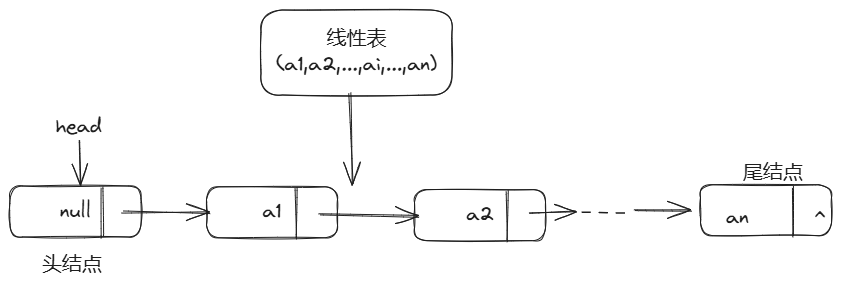
\includegraphics[width=0.8\textwidth]{./image/singleLink.png}
  \caption{单链表表示意图}
  \label{fig:single_linked_list}
\end{figure}

\begin{figure}[!htbp]
  \centering
  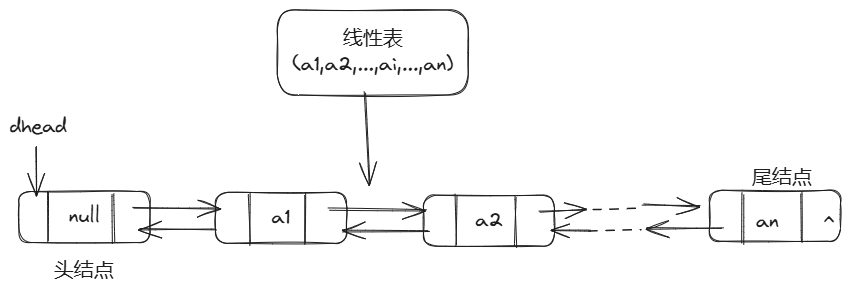
\includegraphics[width=0.8\textwidth]{./image/doubleLink.png}
  \caption{双链表示意图}
  \label{fig:double_linked_list}
\end{figure}

\subsection{单链表}
单链表是链表的一种,每个节点只包含一个数据域和一个指针域,指针指向下一个节点。
\textit{示例}:
$L = \{1001 \rightarrow 1002 \rightarrow 1003\}$。
单链表的结构如图\ref{fig:singleLinkStruct}所示。单链表的结构由数据域和指针域组成,其中数据域存储数据元素,指针域存储下一个节点的地址。
\begin{figure}[!htbp]
  \centering
  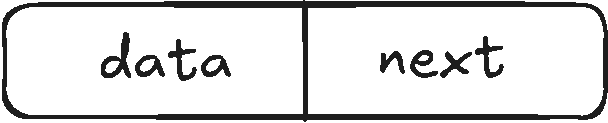
\includegraphics[width=0.4\textwidth]{./figure/pdf/cropped/singleStruct.pdf}
  \caption{单链表结构}
  \label{fig:singleLinkStruct}
\end{figure}
单链表的结构体定义如代码\ref{lst:singleLinkStruct}所示。
\begin{lstlisting}[language=C++, caption={单链表结构体定义}, label={lst:singleLinkStruct}]
  struct ListNode {
    int data;
    ListNode* next;
  };
\end{lstlisting}
单链表的基本操作包括插入、删除、查找和更新。以下是每种操作的详细说明:
建立单链表:

  \textbf{头插法建立单链表}

  1.首先创建一个头结点,将头结点的指针域指向 NULL。
  2.依次读入数据元素,创建新节点,将新节点的指针域指向头结点的下一个节点,再将头结点的指针域指向新节点。
  具体过程如图\ref{fig:headInsert}所示。
  \begin{figure}[!htbp]
    \centering
    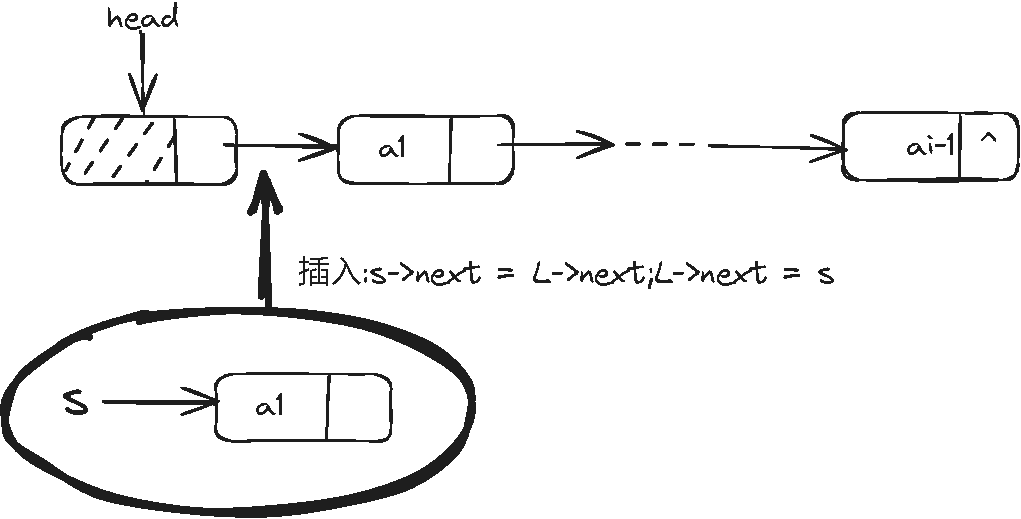
\includegraphics[width=1\textwidth]{./figure/pdf/cropped/headInsert.pdf}
    \caption{头插法建立单链表}
    \label{fig:headInsert}
  \end{figure}
  代码如代码\ref{lst:headInsert}所示。
  \begin{lstlisting}[language=C++, caption={头插法建立单链表示例代码}, label={lst:headInsert}]
    singleLink* createSingleLink() {
      int n, data;
      printf(``请输入创建链表的节点个数:``);
      scanf(``%d``, &n);
      SingleLink* L = (SingleLink*)malloc(sizeof(SingleLink));
      L->next = NULL;
      for (int i = 0; i < n; i++) {
        SingleLink* s = (singleLink*)malloc(sizeof(SingleLink));
        printf(``请输入第%d个节点的值(int):``, i + 1);
        scanf(``%d``, &data);
        s->data = data;
        s->next = NULL;
        s->next = L->next;
        L->next = s;
      }
      return L;
    }
    \end{lstlisting}
    该算法的总时间复杂度为 $O(n)$,空间复杂度为 $O(1)$。

    特点:头插法建立的单链表,新节点插入到链表的头部,逆序存储数据。

  \textbf{尾插法建立单链表}

  1.首先创建一个头结点,将头结点的指针域指向 NULL。
  2.依次读入数据元素,创建新节点,将新节点的指针域指向 NULL,再将尾结点的指针域指向新节点,再将新节点作为尾结点。
  具体过程如图\ref{fig:tailInsert}所示。
  \begin{figure}[!htbp]
    \centering
    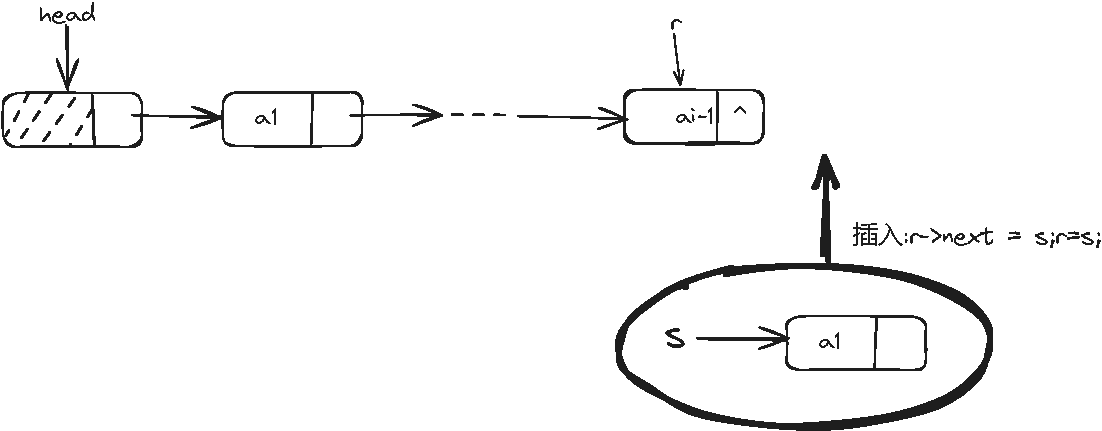
\includegraphics[width=1\textwidth]{./figure/pdf/cropped/tailInsert.pdf}
    \caption{尾插法建立单链表}
    \label{fig:tailInsert}
  \end{figure}
  代码如代码\ref{lst:tailInsert}所示。
  \begin{lstlisting}[language=C++, caption={尾插法建立单链表示例代码}, label={lst:tailInsert}]
    singleLink* createSingleLink() {
      int n, data;
      printf(``请输入创建链表的节点个数:``);
      scanf(``%d``, &n);
      SingleLink* L = (SingleLink*)malloc(sizeof(SingleLink));
      SingleLink* r = L;
      for (int i = 0; i < n; i++) {
        SingleLink* s = (singleLink*)malloc(sizeof(SingleLink));
        printf(``请输入第%d个节点的值(int):``, i + 1);
        scanf(``%d``, &data);
        s->data = data;
        s->next = NULL;
        r->next = s;
        r = s;
      }
      return L;
    }
    \end{lstlisting}
    该算法的总时间复杂度为 $O(n)$,空间复杂度为 $O(1)$。

    特点:尾插法建立的单链表,新节点插入到链表的尾部,顺序存储数据。

    \textbf{创建空链表}
创建一个空链表,只需要创建一个头结点,将头结点的指针域指向 NULL。

代码如代码\ref{lst:createEmptySingleLink}所示。
\begin{lstlisting}[language=C++, caption={创建一个空链表示例代码}, label={lst:createEmptySingleLink}]
  singleLink* createEmptySingleLink() {
    SingleLink* L = (SingleLink*)malloc(sizeof(SingleLink));
    L->next = NULL;
    return L;
  }
\end{lstlisting}
该算法的总时间复杂度为 $O(1)$,空间复杂度为 $O(1)$。

特点:创建的链表为空,不包含任何数据元素。

\textbf{输出单链表}

输出单链表的所有数据元素,需要遍历链表的所有节点,并依次输出节点的数据域。

代码如代码\ref{lst:printSingleLink}所示。

\begin{lstlisting}[language=C++, caption={输出单链表示例代码}, label={lst:printSingleLink}]
void printSingleLink(SingleLink* L) {
  SingleLink* p = L->next;
  while (p != NULL) {
    printf(``%d ``, p->data);
    p = p->next;
  }
  printf(``\n``);
}
\end{lstlisting}
该算法的总时间复杂度为 $O(n)$,空间复杂度为 $O(1)$。

特点:输出单链表的所有数据元素。

\textbf{输出单链表的长度}

输出单链表的长度,需要遍历链表的所有节点,并统计节点的个数。

代码如代码\ref{lst:lengthSingleLink}所示。

\begin{lstlisting}[language=C++, caption={输出单链表长度示例代码}, label={lst:lengthSingleLink}]
int lengthSingleLink(SingleLink* L) {
  SingleLink* p = L->next;
  int length = 0;
  while (p != NULL) {
    length++;
    p = p->next;
  }
  return length;
}
\end{lstlisting}
该算法的总时间复杂度为 $O(n)$,空间复杂度为 $O(1)$。

特点:输出单链表的长度,即链表中数据元素的个数。

\textbf{判断单链表是否为空}

判断单链表是否为空,只需要判断头结点的指针域是否为 NULL。

代码如代码\ref{lst:isEmptySingleLink}所示。

\begin{lstlisting}[language=C++, caption={判断单链表是否为空示例代码}, label={lst:isEmptySingleLink}]
  bool isEmptySingleLink(SingleLink* L) {
    return L->next == NULL;
  }
  \end{lstlisting}
  该算法的总时间复杂度为 $O(1)$,空间复杂度为 $O(1)$。

  特点:判断单链表是否为空,即链表中是否包含数据元素。

\textbf{查找单链表的第 $i$ 个元素}

查找单链表的第 $i$ 个元素,需要遍历链表的所有节点,直到找到第 $i$ 个节点。

代码如代码\ref{lst:getSingleLink}所示。

\begin{lstlisting}[language=C++, caption={查找单链表的第 $i$ 个元素示例代码}, label={lst:getSingleLink}]
  int getSingleLink(SingleLink* L, int i) {
    SingleLink* p = L->next;
    int j = 1;
    while (p != NULL && j < i) {
      p = p->next;
      j++;
    }
    if (p == NULL || j > i) {
      printf(``第%d个元素不存在``, i);
      return -1;
    }
    return p->data;
  }
\end{lstlisting}
该算法的总时间复杂度为 $O(n)$,空间复杂度为 $O(1)$。

特点:查找单链表的第 $i$ 个元素,即链表中第 $i$ 个节点的数据元素。

\textbf{删除单链表的第 $i$ 个元素}

删除单链表的第 $i$ 个元素,需要遍历链表的所有节点,直到找到第 $i$ 个节点,然后删除该节点。

代码如代码\ref{lst:deleteSingleLink}所示。

\begin{lstlisting}[language=C++, caption={删除单链表的第 $i$ 个元素示例代码}, label={lst:deleteSingleLink}]
  void deleteSingleLink(SingleLink* L, int i) {
    SingleLink* p = L;
    for (int j = 0; j < i - 1; j++) {
      p = p->next;
    }
    SingleLink* q = p->next;
    p->next = q->next;
    free(q);
  }
  \end{lstlisting}
  该算法的总时间复杂度为 $O(n)$,空间复杂度为 $O(1)$。

  特点:删除单链表的第 $i$ 个元素,即删除链表中第 $i$ 个节点。

\textbf{插入单链表的第 $i$ 个元素}

插入单链表的第 $i$ 个元素,需要遍历链表的所有节点,直到找到第 $i$ 个节点,然后插入新节点。

代码如代码\ref{lst:insertSingleLink}所示。

\begin{lstlisting}[language=C++, caption={插入单链表的第 $i$ 个元素示例代码}, label={lst:insertSingleLink}]
void insertSingleLink(SingleLink* L, int i, int data) {
  SingleLink* p = L;
  for (int j = 0; j < i - 1; j++) {
    p = p->next;
  }
  SingleLink* s = (SingleLink*)malloc(sizeof(SingleLink));
  s->data = data;
  s->next = p->next;
  p->next = s;
}
\end{lstlisting}
该算法的总时间复杂度为 $O(n)$,空间复杂度为 $O(1)$。

特点:插入单链表的第 $i$ 个元素,即在链表中第 $i$ 个节点的位置插入新节点。
   



  \subsection{双链表}
  单链表只有指向下一个节点的指针,在某一些应用场合可能并不是那么方便,比如在删除某个节点时,需要找到该节点的前驱节点,而单链表并没有指向前驱节点的指针。双链表就是为了解决这个问题而设计的,它的每个节点有两个指针,一个指向前驱节点,一个指向后继节点。
  
  \textit{示例}:
  $L = \{\text{NULL} \leftrightarrow 1001 \leftrightarrow 1002 \leftrightarrow 1003 \leftrightarrow \text{NULL}\}$。

  双链表的结构如图\ref{fig:doubleLinkStruct}所示。双链表的结构由数据域、前驱指针和后继指针组成,其中数据域存储数据元素,前驱指针指向前一个节点,后继指针指向后一个节点。
  \begin{figure}[!htbp]
    \centering
    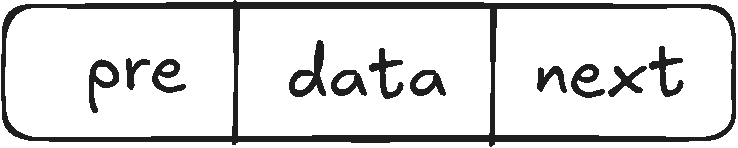
\includegraphics[width=0.4\textwidth]{./figure/pdf/cropped/doubleLinkStruct.pdf}
    \caption{双链表结构}
    \label{fig:doubleLinkStruct}
  \end{figure}

  双链表的结构体定义如代码\ref{lst:doubleLinkStruct}所示。
  \begin{lstlisting}[language=C++, caption={双链表结构体定义}, label={lst:doubleLinkStruct}]
    struct DLink {
      int data;
      DLink* pre;
      DLink* next;
    };
  \end{lstlisting}

  双链表的基本操作包括插入、删除、查找和更新。以下是每种操作的详细说明:

  \textbf{创建操作}:

  创建一个空的双链表,只需要创建一个头结点,将头结点的前驱指针和后继指针都指向 NULL。

  代码如代码\ref{lst:createEmptyDoubleLink}所示。
  \begin{lstlisting}[language=C++, caption={创建一个空双链表示例代码}, label={lst:createEmptyDoubleLink}]
    DLink* createEmptyDoubleLink() {
      DLink* L = (DLink*)malloc(sizeof(DLink));
      L->pre = NULL;
      L->next = NULL;
      return L;
    }
  \end{lstlisting}
  该算法的总时间复杂度为 $O(1)$,空间复杂度为 $O(1)$。

  特点:创建的双链表为空,不包含任何数据元素。

  \textbf{头插法}:

  头插法建立双链表,新节点插入到链表的头部。

  1.首先创建一个头结点,将头结点的前驱指针和后继指针都指向 NULL。

  2.依次读入数据元素,创建新节点,将新节点的前驱指针指向头结点,将新节点的后继指针指向头结点的后继节点,再将头结点的后继指针指向新节点,最后将新节点作为头结点的后继节点。

  具体过程如图\ref{fig:headInsertDouble}所示。
  \begin{figure}[!htbp]
    \centering
    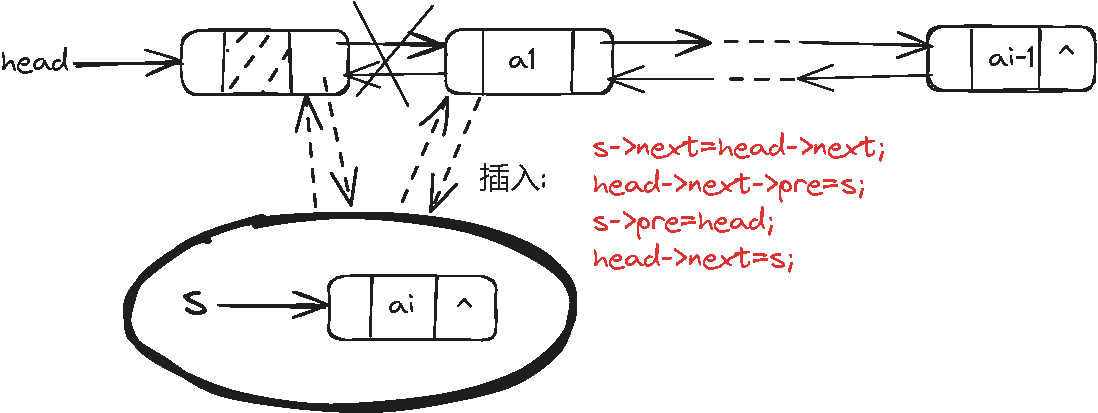
\includegraphics[width=1\textwidth]{./figure/pdf/cropped/headInsertDL.pdf}
    \caption{头插法建立双链表}
    \label{fig:headInsertDouble}
  \end{figure}
  代码如代码\ref{lst:headInsertDouble}所示。
  \begin{lstlisting}[language=C++, caption={头插法建立双链表示例代码}, label={lst:headInsertDouble}]
    DLink* createDoubleLink() {
      int n, data;
      printf(``请输入创建链表的节点个数:``);
      scanf(``%d``, &n);
      DLink* L = (DLink*)malloc(sizeof(DLink));
      L->pre = NULL;
      L->next = NULL;
      for (int i = 0; i < n; i++) {
        DLink* s = (DLink*)malloc(sizeof(DLink));
        printf(``请输入第%d个节点的值(int):``, i + 1);
        scanf(``%d``, &data);
        s->data = data;
        s->pre = L;
        s->next = L->next;
        L->next = s;
      }
      return L;
    }
  \end{lstlisting}
  该算法的总时间复杂度为 $O(n)$,空间复杂度为 $O(1)$。
 
  \textbf{尾插法}:
  尾插法建立双链表,新节点插入到链表的尾部。

  1.首先创建一个头结点,将头结点的前驱指针和后继指针都指向 NULL。

  2.依次读入数据元素,创建新节点,将新节点的前驱指针指向尾结点,将新节点的后继指针指向 NULL,再将尾结点的后继指针指向新节点,最后将新节点作为尾结点。

  具体过程如图\ref{fig:tailInsertDouble}所示。
  \begin{figure}[!htbp]
    \centering
    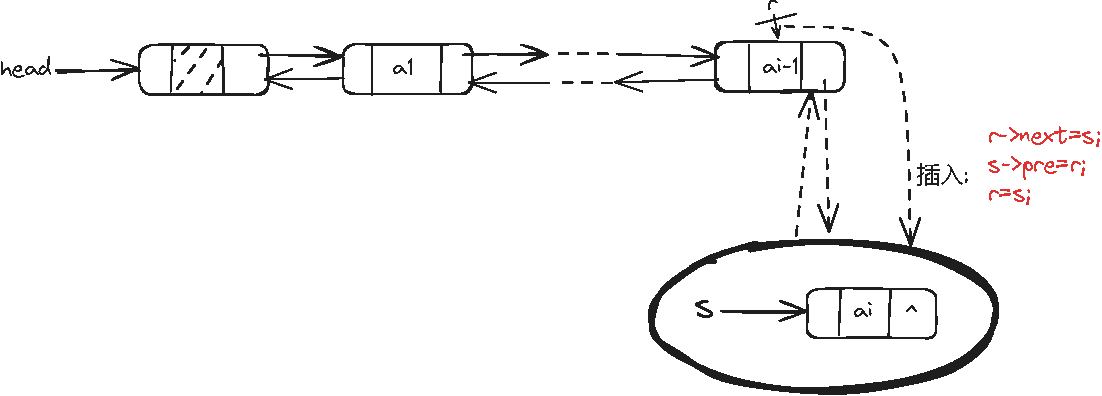
\includegraphics[width=1\textwidth]{./figure/pdf/cropped/tailInsertDL.pdf}
    \caption{尾插法建立双链表}
    \label{fig:tailInsertDouble}
  \end{figure}
  代码如代码\ref{lst:tailInsertDouble}所示。

  \begin{lstlisting}[language=C++, caption={尾插法建立双链表示例代码}, label={lst:tailInsertDouble}]
    DLink* createDoubleLink() {
      int n, data;
      printf(``请输入创建链表的节点个数:``);
      scanf(``%d``, &n);
      DLink* L = (DLink*)malloc(sizeof(DLink));
      DLink* r = L;
      for (int i = 0; i < n; i++) {
        DLink* s = (DLink*)malloc(sizeof(DLink));
        printf(``请输入第%d个节点的值(int):``, i + 1);
        scanf(``%d``, &data);
        s->data = data;
        s->pre = r;
        s->next = NULL;
        r->next = s;
        r = s;
      }
      return L;
    }
  \end{lstlisting}
  该算法的总时间复杂度为 $O(n)$,空间复杂度为 $O(1)$。

  特点:尾插法建立的双链表,新节点插入到链表的尾部,顺序存储数据。

  \textbf{输出操作}:

  输出双链表的所有数据元素,需要遍历链表的所有节点,并依次输出节点的数据域。

  代码如代码\ref{lst:printDoubleLink}所示。

  \begin{lstlisting}[language=C++, caption={输出双链表示例代码}, label={lst:printDoubleLink}]
    void printDoubleLink(DLink* L) {
      DLink* p = L->next;
      while (p != NULL) {
        printf(``%d ``, p->data);
        p = p->next;
      }
      printf(``\n``);
    }
  \end{lstlisting}

  该算法的总时间复杂度为 $O(n)$,空间复杂度为 $O(1)$。

  特点:输出双链表的所有数据元素。

  \textbf{输出双链表的长度}:

  输出双链表的长度,需要遍历链表的所有节点,并统计节点的个数。

  代码如代码\ref{lst:lengthDoubleLink}所示。

  \begin{lstlisting}[language=C++, caption={输出双链表长度示例代码}, label={lst:lengthDoubleLink}]
    int lengthDoubleLink(DLink* L) {
      DLink* p = L->next;
      int length = 0;
      while (p != NULL) {
        length++;
        p = p->next;
      }
      return length;
    }
  \end{lstlisting}

  该算法的总时间复杂度为 $O(n)$,空间复杂度为 $O(1)$。

  特点:输出双链表的长度,即链表中数据元素的个数。

  \textbf{判断双链表是否为空}:

  判断双链表是否为空,只需要判断头结点的后继指针是否为 NULL。

  代码如代码\ref{lst:isEmptyDoubleLink}所示。

  \begin{lstlisting}[language=C++, caption={判断双链表是否为空示例代码}, label={lst:isEmptyDoubleLink}]
    bool isEmptyDoubleLink(DLink* L) {
      return L->next == NULL;
    }
  \end{lstlisting}

  该算法的总时间复杂度为 $O(1)$,空间复杂度为 $O(1)$。

  特点:判断双链表是否为空,即链表中是否包含数据元素。

  \textbf{查找双链表的第 $i$ 个元素}:

  查找双链表的第 $i$ 个元素,需要遍历链表的所有节点,直到找到第 $i$ 个节点。

  代码如代码\ref{lst:getDoubleLink}所示。

  \begin{lstlisting}[language=C++, caption={查找双链表的第 $i$ 个元素示例代码}, label={lst:getDoubleLink}]
    int getDoubleLink(DLink* L, int i) {
      DLink* p = L->next;
      int j = 1;
      while (p != NULL && j < i) {
        p = p->next;
        j++;
      }
      if (p == NULL || j > i) {
        printf(``第%d个元素不存在``, i);
        return -1;
      }
      return p->data;
    }
  \end{lstlisting}

  该算法的总时间复杂度为 $O(n)$,空间复杂度为 $O(1)$。

  特点:查找双链表的第 $i$ 个元素,即链表中第 $i$ 个节点的数据元素。

  \textbf{删除双链表的第 $i$ 个元素}:

  删除双链表的第 $i$ 个元素,需要遍历链表的所有节点,直到找到第 $i$ 个节点,然后删除该节点。

  代码如代码\ref{lst:deleteDoubleLink}所示。

  \begin{lstlisting}[language=C++, caption={删除双链表的第 $i$ 个元素示例代码}, label={lst:deleteDoubleLink}]
    void deleteDoubleLink(DLink* L, int i) {
      DLink* p = L;
      for (int j = 0; j < i - 1; j++) {
        p = p->next;
      }
      DLink* q = p->next;
      p->next = q->next;
      if (q->next != NULL) {
        q->next->pre = p;
      }
      free(q);
    }
  \end{lstlisting}

  该算法的总时间复杂度为 $O(n)$,空间复杂度为 $O(1)$。

  特点:删除双链表的第 $i$ 个元素,即删除链表中第 $i$ 个节点。

  \textbf{插入双链表的第 $i$ 个元素}:

  插入双链表的第 $i$ 个元素,需要遍历链表的所有节点,直到找到第 $i$ 个节点,然后插入新节点。

  其中删除操作如图\ref{fig:deleteDoubleLink}所示。

  \begin{figure}[!htbp]
    \centering
    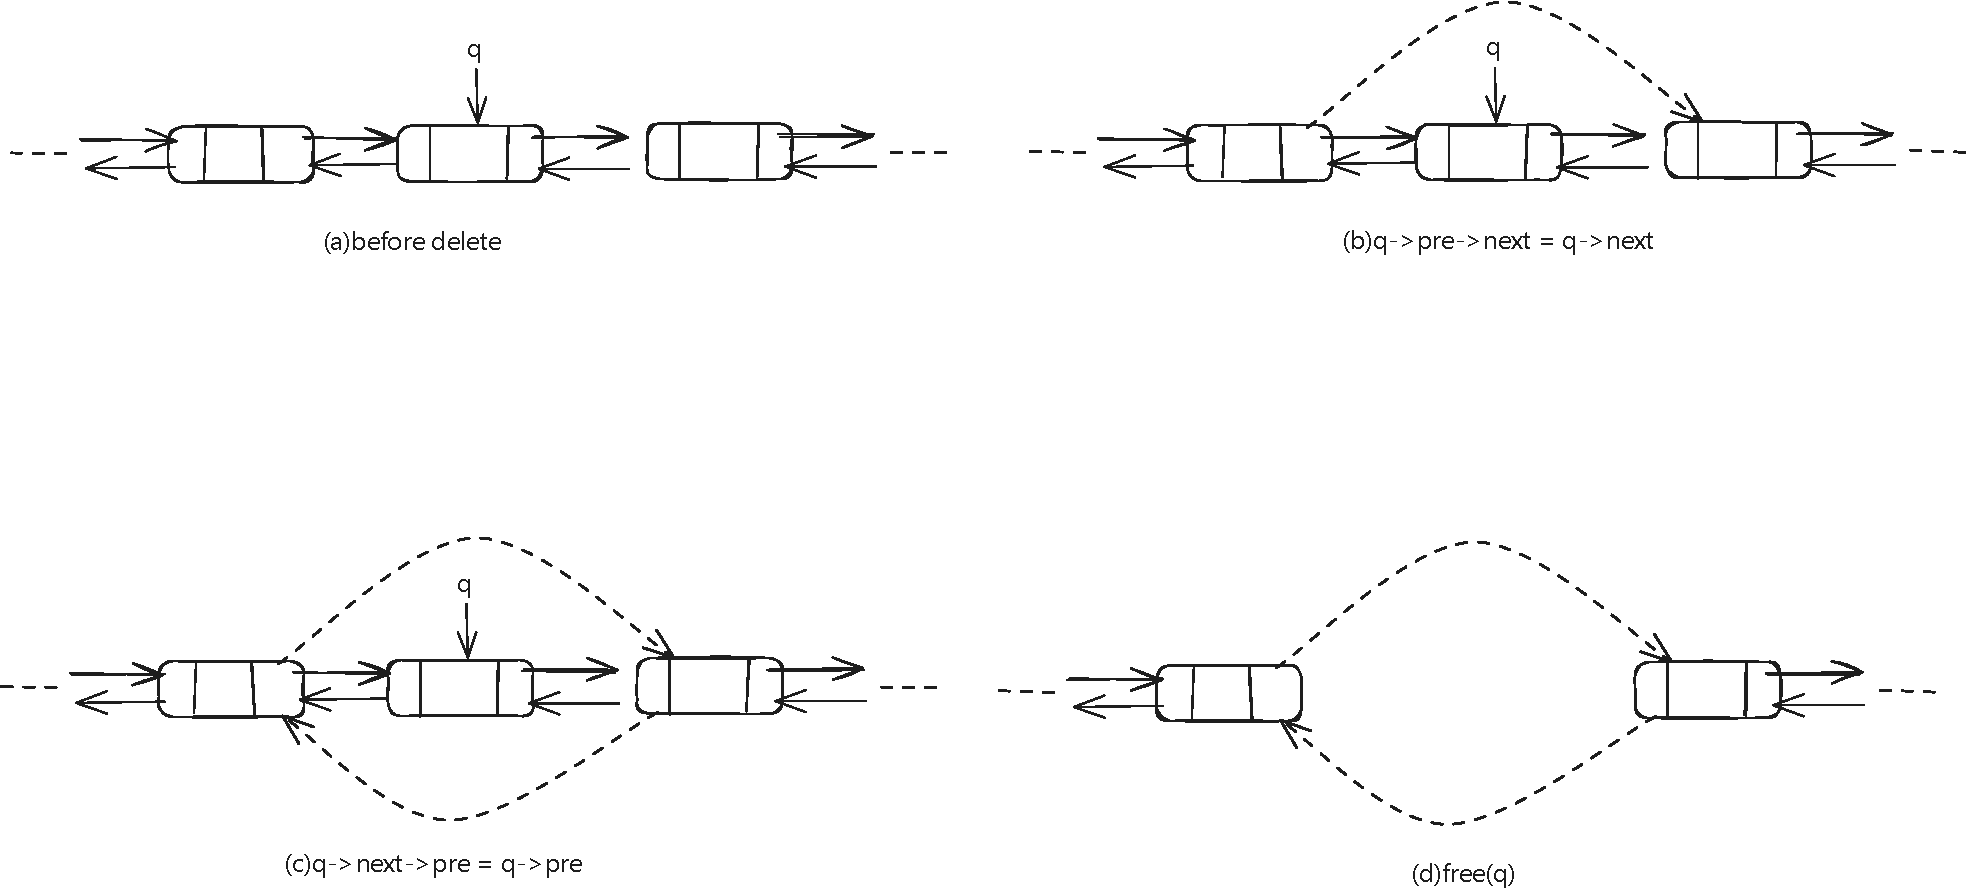
\includegraphics[width=1\textwidth]{./figure/pdf/cropped/deleteDL.pdf}
    \caption{删除双链表的第 $i$ 个元素}
    \label{fig:deleteDoubleLink}
  \end{figure}

  代码如代码\ref{lst:insertDoubleLink}所示。

  \begin{lstlisting}[language=C++, caption={插入双链表的第 $i$ 个元素示例代码}, label={lst:insertDoubleLink}]
    void insertDoubleLink(DLink* L, int i, int data) {
      DLink* p = L;
      for (int j = 0; j < i - 1; j++) {
        p = p->next;
      }
      DLink* s = (DLink*)malloc(sizeof(DLink));
      s->data = data;
      s->pre = p;
      s->next = p->next;
      if (p->next != NULL) {
        p->next->pre = s;
      }
      p->next = s;
    }

  \end{lstlisting}

  该算法的总时间复杂度为 $O(n)$,空间复杂度为 $O(1)$。

  特点:插入双链表的第 $i$ 个元素,即在链表中第 $i$ 个节点的位置插入新节点。

  \textbf{p结点之后插入结点s}:

  过程如图\ref{fig:insertAfterDoubleLink}所示。

  \begin{figure}[!htbp]
    \centering
    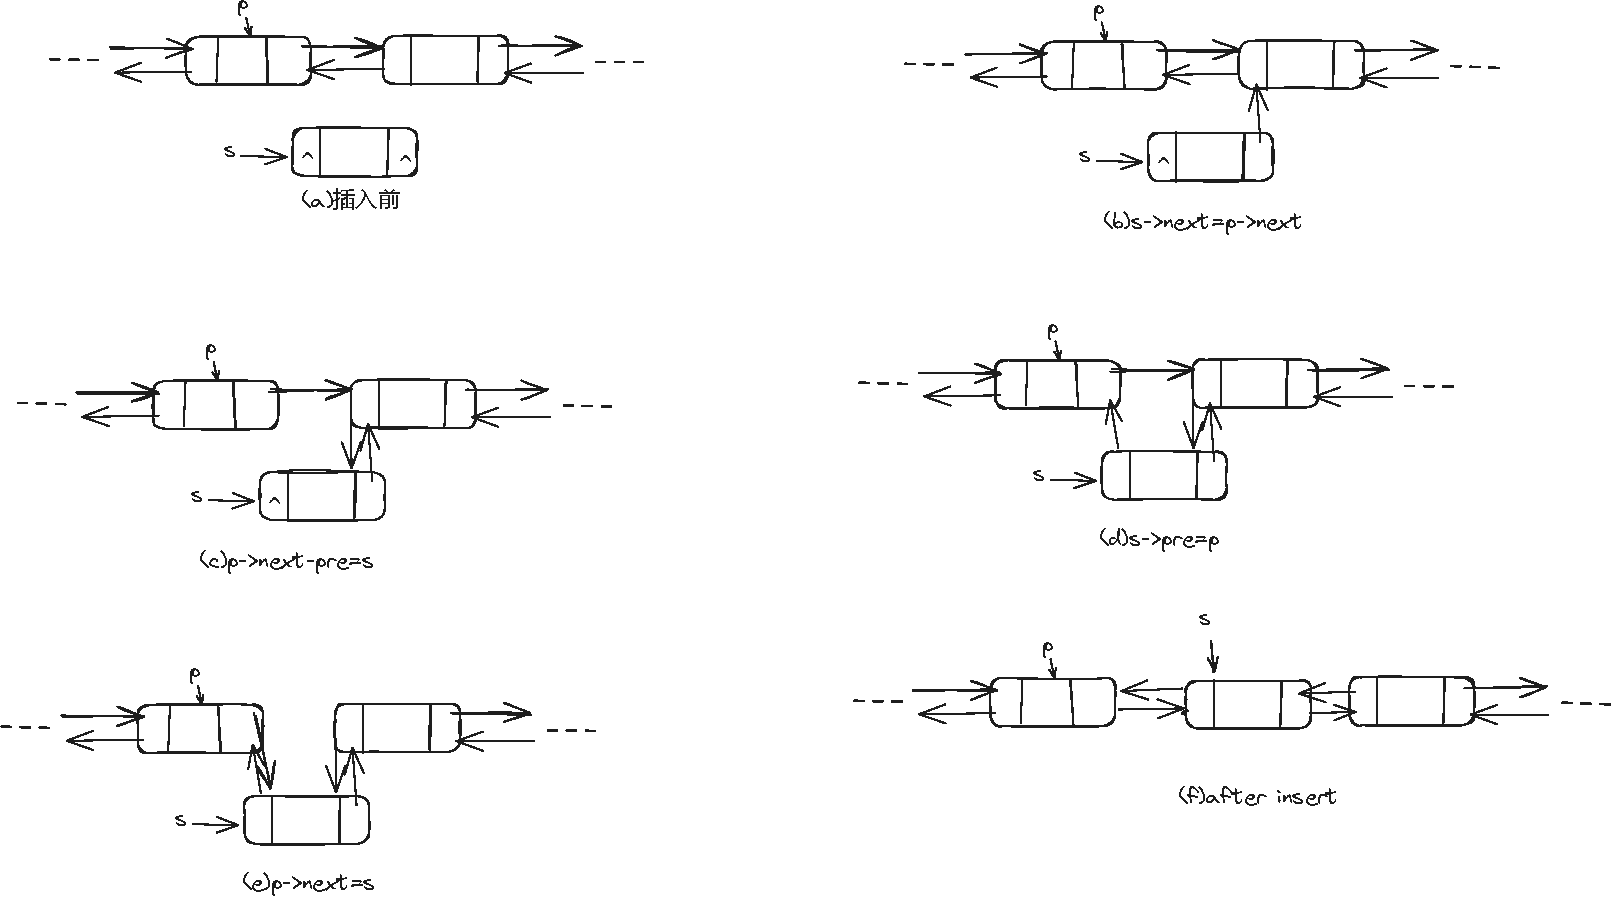
\includegraphics[width=1\textwidth]{./figure/pdf/cropped/insertDL.pdf}
    \caption{p结点之后插入结点s}
    \label{fig:insertAfterDoubleLink}
  \end{figure}
  代码如代码\ref{lst:insertAfterDoubleLink}所示。

  \begin{lstlisting}[language=C++, caption={p结点之后插入结点s示例代码}, label={lst:insertAfterDoubleLink}]
    void insertAfterDoubleLink(DLink* p, DLink* s) {
      s->pre = p;
      s->next = p->next;
      if (p->next != NULL) {
        p->next->pre = s;
      }
      p->next = s;
    }
  \end{lstlisting}

  该算法的总时间复杂度为 $O(1)$,空间复杂度为 $O(1)$。

  特点:在双链表中结点 p 之后插入结点 s。



  \subsection{循环链表\&静态链表}
  循环链表是链表的一种,最后一个节点的指针指向第一个节点,形成一个环。
  \textit{示例}:
  $L = \{1001 \rightarrow 1002 \rightarrow 1003 \rightarrow 1001\}$。

  \textbf{循环单链表}:

  循环单链表和单链表的区别在于,循环单链表的尾结点指针指向头结点。

  其结构如图\ref{fig:cycleSingleLink}所示。

  \begin{figure}[!htbp]
    \centering
    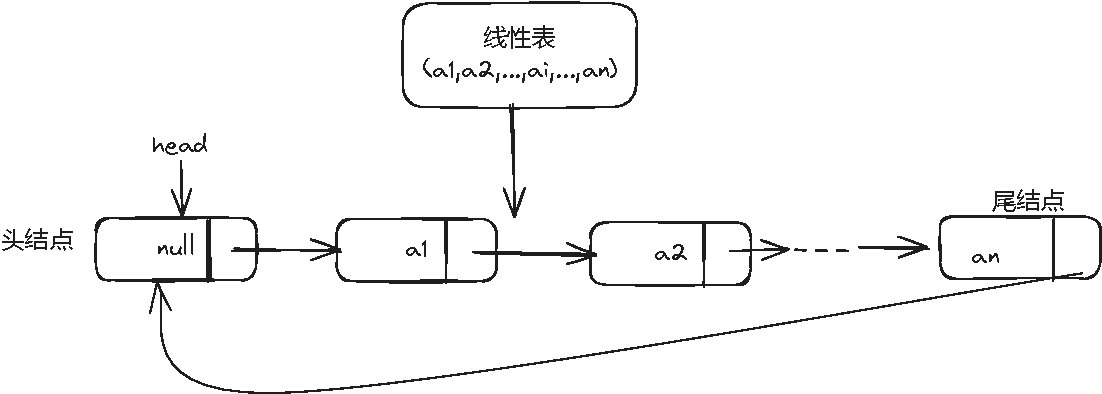
\includegraphics[width=0.6\textwidth]{./figure/pdf/cropped/cycleSLink.pdf}
    \caption{循环单链表结构}
    \label{fig:cycleSingleLink}
  \end{figure}

  \textbf{循环双链表}:

  循环双链表和双链表的区别在于,循环双链表的头结点的前驱指针指向尾结点,尾结点的后继指针指向头结点。

  其结构如图\ref{fig:cycleDoubleLink}所示。

  \begin{figure}[!htbp]
    \centering
    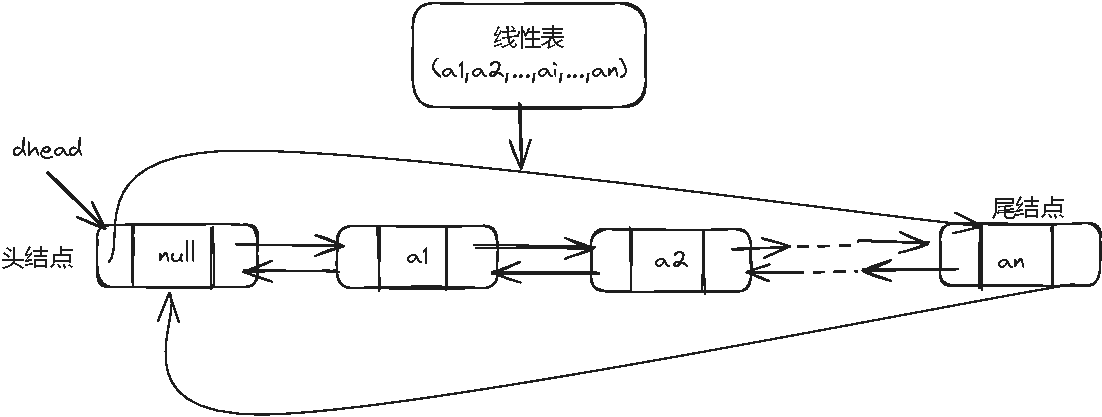
\includegraphics[width=0.6\textwidth]{./figure/pdf/cropped/cycleDLink.pdf}
    \caption{循环双链表结构}
    \label{fig:cycleDoubleLink}
  \end{figure}


  静态链表是使用数组模拟链表的一种实现方式,每个数组元素包含数据域和指针域。与前面所讲的链表不同,静态链表的指针域
  存储的是数组的索引,而不是指向下一个节点的指针。静态链表和顺序表一样,使用数组存储数据元素,但是静态链表可以更好地支持插入和删除操作。

  如图\ref{fig:staticLink}所示,静态链表的结构由数据域和指针域组成,其中数据域存储数据元素,指针域存储数组的索引。

  \begin{figure}[!htbp]
    \centering
    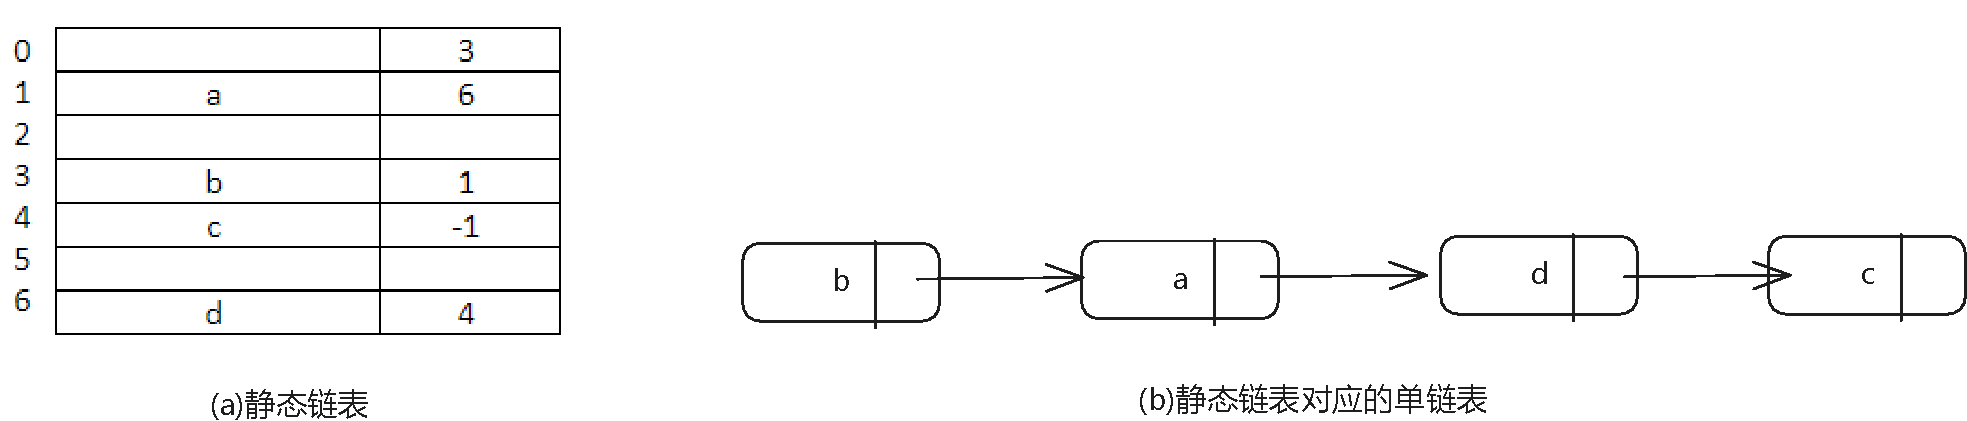
\includegraphics[width=1\textwidth]{./figure/pdf/cropped/staticLink.pdf}
    \caption{静态链表结构}
    \label{fig:staticLink}
  \end{figure}

 数组的第一个元素不存储数据,它的指针域存储第一个数据元素的索引,最后一个元素的指针域存储下一个空闲位置的索引。最后一个
 元素的指针域值为-1。

  \section{顺序表与链表的比较}
  \begin{itemize}
      \item \textbf{存储方式}:顺序表使用数组存储数据元素,链表使用指针存储数据元素。
      \item \textbf{插入和删除}:顺序表插入和删除操作需要移动元素,时间复杂度为 $O(n)$,链表插入和删除操作只需要修改指针,时间复杂度为 $O(1)$。
      \item \textbf{空间复杂度}:顺序表的空间复杂度为 $O(n)$,链表的空间复杂度为 $O(n)$。
      \item \textbf{访问速度}:顺序表的访问速度快,时间复杂度为 $O(1)$,链表的访问速度慢,时间复杂度为 $O(n)$。
  \end{itemize}




\textit{总结}:顺序表适合需要频繁访问的场景,而链表适合需要频繁插入和删除的场景。

\chapter{栈与队列}
从组成元素的逻辑关系来看,栈和队列都属于线性结构.栈和队列与线性表的不同之处在于它们的相关运算具有一些特殊性.
更准确地说,一般线性表上的插入/删除运算不受限制,而栈和队列上的插入 删除运算均会受到某种特殊限制,
因此栈和队列也称为操作受限的线性表.
\section{栈}

\subsection{栈的定义}

栈是一种特殊的线性表,只能在表的一端进行插入和删除操作。栈的插入操作称为入栈,删除操作称为出栈。栈的特点是后进先出,即最后入栈的元素最先出栈。

如图\ref{fig:stack}所示,栈的结构由栈顶和栈底组成,栈顶指向栈顶元素,栈底指向栈底元素。

\begin{figure}[!htbp]
  \centering
  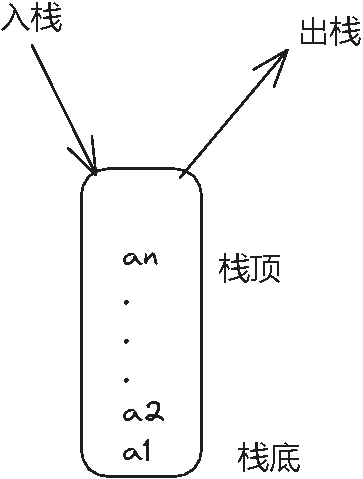
\includegraphics[width=0.2\textwidth]{./figure/pdf/cropped/stack.pdf}
  \caption{栈结构}
  \label{fig:stack}
\end{figure}

相关术语:

\begin{itemize}
  \item \textbf{栈顶}:栈顶是栈中最后一个元素。
  \item \textbf{栈底}:栈底是栈中第一个元素。
  \item \textbf{空栈}:栈中不包含任何元素。
  \item \textbf{满栈}:栈中包含的元素个数等于栈的最大容量。
  \item \textbf{栈的大小}:栈中包含的元素个数。
  \item \textbf{栈的容量}:栈的最大容量。
  \item \textbf{栈的压入}:将元素压入栈中。
  \item \textbf{栈的弹出}:将元素从栈中弹出。
  \end{itemize}

栈的特点:

\begin{itemize}
  \item 栈是一种特殊的线性表,只能在表的一端进行插入和删除操作。
  \item 栈的插入操作称为入栈,删除操作称为出栈。
  \item 栈的特点是后进先出,即最后入栈的元素最先出栈。
\end{itemize}
\subsection{栈的操作}

栈的基本操作包括创建、销毁、压入、弹出、获取栈顶元素、判断栈是否为空、判断栈是否为满、获取栈的大小和获取栈的容量。

\begin{itemize}
  \item \textbf{创建操作}:创建一个空栈。
  \item \textbf{销毁操作}:销毁栈。
  \item \textbf{压入操作}:将元素压入栈中。
  \item \textbf{弹出操作}:将元素从栈中弹出。
  \item \textbf{获取栈顶元素}:获取栈顶元素。
  \item \textbf{判断栈是否为空}:判断栈中是否包含元素。
  \item \textbf{判断栈是否为满}:判断栈中是否包含元素。
  \item \textbf{获取栈的大小}:获取栈中包含的元素个数。
  \item \textbf{获取栈的容量}:获取栈的最大容量。
  \item \textbf{清空栈}:清空栈中的所有元素。
  \item \textbf{遍历栈}:遍历栈中的所有元素。
\end{itemize}


\subsection{顺序栈}

顺序栈是使用数组实现的栈,栈的大小是固定的,栈的容量是数组的大小。

顺序栈的结构体定义如代码\ref{lst:seqStackStruct}所示。

\begin{lstlisting}[language=C++, caption={顺序栈结构体定义}, label={lst:seqStackStruct}]
  struct SeqStack {
    int* data;//栈的数据元素
    int top;//栈顶指针
    int capacity;//栈的容量
  };
\end{lstlisting}

顺序栈的存放过程如图\ref{fig:seqStack}所示。

\begin{figure}[!htbp]
  \centering
  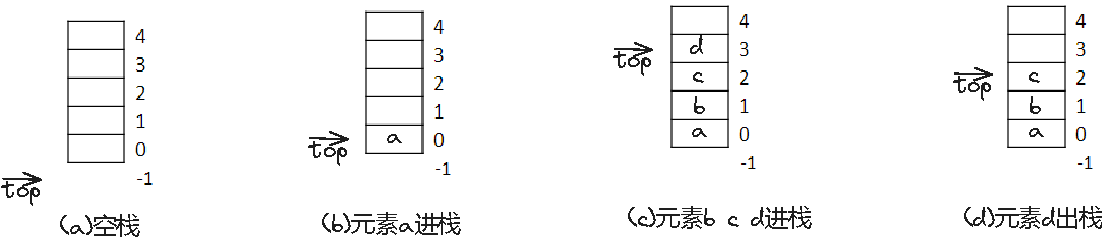
\includegraphics[width=1\textwidth]{./figure/pdf/cropped/processOfSeqStack.pdf}
  \caption{顺序栈存放过程}
  \label{fig:seqStack}
\end{figure}

顺序栈的基本操作包括创建、销毁、压入、弹出、获取栈顶元素、判断栈是否为空、判断栈是否为满、获取栈的大小和获取栈的容量。

\textbf{创建操作}:

创建一个空的顺序栈,需要为栈分配内存空间,并初始化栈的大小、栈的容量和栈顶指针。

代码如代码\ref{lst:createSeqStack}所示。

\begin{lstlisting}[language=C++, caption={创建一个空顺序栈示例代码}, label={lst:createSeqStack}]
  SeqStack* createSeqStack(int capacity) {
    SeqStack* S = (SeqStack*)malloc(sizeof(SeqStack));
    S->data = (int*)malloc(sizeof(int) * capacity);
    S->top = -1;
    S->capacity = capacity;
    return S;
  }

\end{lstlisting}

该算法的总时间复杂度为 $O(1)$,空间复杂度为 $O(n)$。

特点:创建的顺序栈为空,不包含任何数据元素。

\textbf{销毁操作}:

销毁顺序栈,需要释放栈的内存空间。

代码如代码\ref{lst:destroySeqStack}所示。

\begin{lstlisting}[language=C++, caption={销毁顺序栈示例代码}, label={lst:destroySeqStack}]
  void destroySeqStack(SeqStack* S) {
    free(S->data);
    free(S);
  }
\end{lstlisting}

该算法的总时间复杂度为 $O(1)$,空间复杂度为 $O(1)$。

特点:销毁顺序栈,释放栈的内存空间。

\textbf{判满操作}:

判断顺序栈是否为满,即栈中包含的元素个数等于栈的容量。

代码如代码\ref{lst:isFullSeqStack}所示。

\begin{lstlisting}[language=C++, caption={判断顺序栈是否为满示例代码}, label={lst:isFullSeqStack}]
  bool isFullSeqStack(SeqStack* S) {
    return S->top == S->capacity - 1;
  }

\end{lstlisting}

该算法的总时间复杂度为 $O(1)$,空间复杂度为 $O(1)$。

特点:判断顺序栈是否为满,即栈中包含的元素个数等于栈的容量。

\textbf{判空操作}:

判断顺序栈是否为空,即栈中不包含任何元素。

代码如代码\ref{lst:isEmptySeqStack}所示。

\begin{lstlisting}[language=C++, caption={判断顺序栈是否为空示例代码}, label={lst:isEmptySeqStack}]
  bool isEmptySeqStack(SeqStack* S) {
    return S->top == -1;
  }

\end{lstlisting}

该算法的总时间复杂度为 $O(1)$,空间复杂度为 $O(1)$。

特点:判断顺序栈是否为空,即栈中不包含任何元素。

\textbf{压入操作}:

将元素压入顺序栈中,即将元素放入栈顶。

代码如代码\ref{lst:pushSeqStack}所示。

\begin{lstlisting}[language=C++, caption={压入顺序栈示例代码}, label={lst:pushSeqStack}]
  void pushSeqStack(SeqStack* S, int data) {
    if (isFullSeqStack(S)) {
      printf(``栈已满,无法压入元素\n``);
      return;
    }
    S->data[++S->top] = data;
  }

\end{lstlisting}

该算法的总时间复杂度为 $O(1)$,空间复杂度为 $O(1)$。

特点:将元素压入顺序栈中,即将元素放入栈顶。

\textbf{弹出操作}:

将元素从顺序栈中弹出,即将栈顶元素删除。

代码如代码\ref{lst:popSeqStack}所示。

\begin{lstlisting}[language=C++, caption={弹出顺序栈示例代码}, label={lst:popSeqStack}]
  void popSeqStack(SeqStack* S) {
    if (isEmptySeqStack(S)) {
      printf(``栈为空,无法弹出元素\n``);
      return;
    }
    S->top--;
  }

\end{lstlisting}

该算法的总时间复杂度为 $O(1)$,空间复杂度为 $O(1)$。

特点:将元素从顺序栈中弹出,即将栈顶元素删除。

\textbf{获取栈顶元素}:

获取顺序栈的栈顶元素,即获取栈顶元素的值。

代码如代码\ref{lst:getTopSeqStack}所示。

\begin{lstlisting}[language=C++, caption={获取顺序栈的栈顶元素示例代码}, label={lst:getTopSeqStack}]
  int getTopSeqStack(SeqStack* S) {
    if (isEmptySeqStack(S)) {
      printf(``栈为空,无法获取栈顶元素\n``);
      return -1;
    }
    return S->data[S->top];
  }

\end{lstlisting}

该算法的总时间复杂度为 $O(1)$,空间复杂度为 $O(1)$。

特点:获取顺序栈的栈顶元素,即获取栈顶元素的值。

\textbf{获取栈的大小}:

获取顺序栈的大小,即获取栈中包含的元素个数。

代码如代码\ref{lst:sizeSeqStack}所示。

\begin{lstlisting}[language=C++, caption={获取顺序栈的大小示例代码}, label={lst:sizeSeqStack}]
  int sizeSeqStack(SeqStack* S) {
    return S->top + 1;
  }

\end{lstlisting}

该算法的总时间复杂度为 $O(1)$,空间复杂度为 $O(1)$。

特点:获取顺序栈的大小,即获取栈中包含的元素个数。

\textbf{获取栈的容量}:

获取顺序栈的容量,即获取栈的最大容量。

代码如代码\ref{lst:capacitySeqStack}所示。

\begin{lstlisting}[language=C++, caption={获取顺序栈的容量示例代码}, label={lst:capacitySeqStack}]
  int capacitySeqStack(SeqStack* S) {
    return S->capacity;
  }

\end{lstlisting}

该算法的总时间复杂度为 $O(1)$,空间复杂度为 $O(1)$。

特点:获取顺序栈的容量,即获取栈的最大容量。

\textbf{清空栈}:

清空顺序栈,即将栈中的所有元素删除。

代码如代码\ref{lst:clearSeqStack}所示。

\begin{lstlisting}[language=C++, caption={清空顺序栈示例代码}, label={lst:clearSeqStack}]
  void clearSeqStack(SeqStack* S) {
    S->top = -1;
  }

\end{lstlisting}

该算法的总时间复杂度为 $O(1)$,空间复杂度为 $O(1)$。

特点:清空顺序栈,即将栈中的所有元素删除。

\textbf{遍历栈}:

遍历顺序栈,即输出栈中的所有元素。

代码如代码\ref{lst:traverseSeqStack}所示。

\begin{lstlisting}[language=C++, caption={遍历顺序栈示例代码}, label={lst:traverseSeqStack}]
  void traverseSeqStack(SeqStack* S) {
    for (int i = 0; i <= S->top; i++) {
      printf(``%d ``, S->data[i]);
    }
    printf(``\n``);
  }

\end{lstlisting}

该算法的总时间复杂度为 $O(n)$,空间复杂度为 $O(1)$。

特点:遍历顺序栈,即输出栈中的所有元素。




\subsection{链栈}

栈是线性表的特例,线性表的存储结构还有链式存储结构,因此栈也可以使用链式存储结构实现,称为链栈.

链栈的结构体定义如代码\ref{lst:linkStackStruct}所示。

\begin{lstlisting}[language=C++, caption={链栈结构体定义}, label={lst:linkStackStruct}]
  struct LinkStack {
    int data;//栈的数据元素
    LinkStack* next;//栈的下一个元素
  };
\end{lstlisting}

链栈结构如图\ref{fig:linkStack}所示。

\begin{figure}[!htbp]
  \centering
  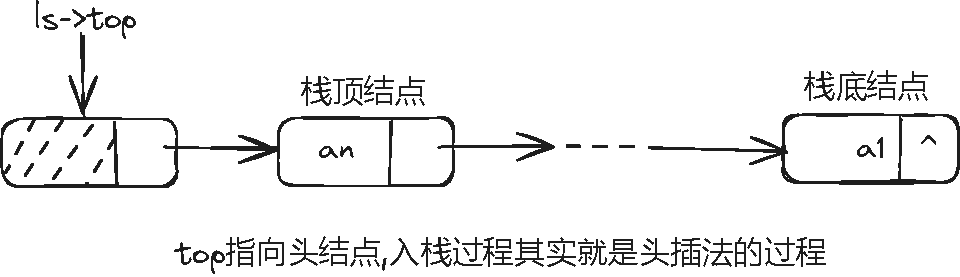
\includegraphics[width=1\textwidth]{./figure/pdf/cropped/linkStack.pdf}
  \caption{链栈}
  \label{fig:linkStack}
\end{figure}

我们可以发现,链栈的结构与单链表的结构相似,只是链栈的操作受到了限制,只能在栈顶进行插入和删除操作。

链栈的基本操作包括创建、销毁、压入、弹出、获取栈顶元素、判断栈是否为空、获取栈的大小和遍历栈。

\textbf{创建操作}:

创建一个空链栈,需要为栈分配内存空间,并初始化栈顶指针。

代码如代码\ref{lst:createLinkStack}所示。

\begin{lstlisting}[language=C++, caption={创建一个空链栈示例代码}, label={lst:createLinkStack}]
  LinkStack* createLinkStack() {
    LinkStack* S = (LinkStack*)malloc(sizeof(LinkStack));
    S->next = NULL;
    return S;
  }

\end{lstlisting}

该算法的总时间复杂度为 $O(1)$,空间复杂度为 $O(1)$。

特点:创建的链栈为空,不包含任何数据元素。

\textbf{销毁操作}:

销毁链栈,需要释放栈的内存空间。

代码如代码\ref{lst:destroyLinkStack}所示。

\begin{lstlisting}[language=C++, caption={销毁链栈示例代码}, label={lst:destroyLinkStack}]
  void destroyLinkStack(LinkStack* S) {
    LinkStack* p = S;
    while (p != NULL) {
      LinkStack* q = p;
      p = p->next;
      free(q);
    }
  }

\end{lstlisting}

该算法的总时间复杂度为 $O(n)$,空间复杂度为 $O(1)$。

特点:销毁链栈,释放栈的内存空间。

\textbf{判空操作}:

判断链栈是否为空,即栈中不包含任何元素。

代码如代码\ref{lst:isEmptyLinkStack}所示。

\begin{lstlisting}[language=C++, caption={判断链栈是否为空示例代码}, label={lst:isEmptyLinkStack}]
  bool isEmptyLinkStack(LinkStack* S) {
    return S->next == NULL;
  }

\end{lstlisting}

该算法的总时间复杂度为 $O(1)$,空间复杂度为 $O(1)$。

特点:判断链栈是否为空,即栈中不包含任何元素。

\textbf{压入操作}:

将元素压入链栈中,即将元素放入栈顶。

代码如代码\ref{lst:pushLinkStack}所示。

\begin{lstlisting}[language=C++, caption={压入链栈示例代码}, label={lst:pushLinkStack}]
  void pushLinkStack(LinkStack* S, int data) {
    LinkStack* p = (LinkStack*)malloc(sizeof(LinkStack));
    p->data = data;
    p->next = S->next;
    S->next = p;
  }

\end{lstlisting}

该算法的总时间复杂度为 $O(1)$,空间复杂度为 $O(1)$。

特点:将元素压入链栈中,即将元素放入栈顶。

\textbf{弹出操作}:

将元素从链栈中弹出,即将栈顶元素删除。

代码如代码\ref{lst:popLinkStack}所示。

\begin{lstlisting}[language=C++, caption={弹出链栈示例代码}, label={lst:popLinkStack}]
  void popLinkStack(LinkStack* S) {
    if (isEmptyLinkStack(S)) {
      printf(``栈为空,无法弹出元素\n``);
      return;
    }
    LinkStack* p = S->next;
    S->next = p->next;
    free(p);
  }

\end{lstlisting}

该算法的总时间复杂度为 $O(1)$,空间复杂度为 $O(1)$。

特点:将元素从链栈中弹出,即将栈顶元素删除。

\textbf{获取栈顶元素}:

获取链栈的栈顶元素,即获取栈顶元素的值。

代码如代码\ref{lst:getTopLinkStack}所示。

\begin{lstlisting}[language=C++, caption={获取链栈的栈顶元素示例代码}, label={lst:getTopLinkStack}]
  int getTopLinkStack(LinkStack* S) {
    if (isEmptyLinkStack(S)) {
      printf(``栈为空,无法获取栈顶元素\n``);
      return -1;
    }
    return S->next->data;
  }

\end{lstlisting}

该算法的总时间复杂度为 $O(1)$,空间复杂度为 $O(1)$。

特点:获取链栈的栈顶元素,即获取栈顶元素的值。

\textbf{遍历栈}:

遍历链栈,即输出栈中的所有元素。

代码如代码\ref{lst:traverseLinkStack}所示。

\begin{lstlisting}[language=C++, caption={遍历链栈示例代码}, label={lst:traverseLinkStack}]
  void traverseLinkStack(LinkStack* S) {
    LinkStack* p = S->next;
    while (p != NULL) {
      printf(``%d ``, p->data);
      p = p->next;
    }
    printf(``\n``);
  }

\end{lstlisting}

该算法的总时间复杂度为 $O(n)$,空间复杂度为 $O(1)$。

特点:遍历链栈,即输出栈中的所有元素。



\subsection{共享栈}

共享栈是两个栈共享一个存储空间的栈,两个栈的栈底分别位于共享空间的两端,两个栈的栈顶向中间延伸。

共享栈的结构如图\ref{fig:sharedStack}所示。

\begin{figure}[!htbp]
  \centering
  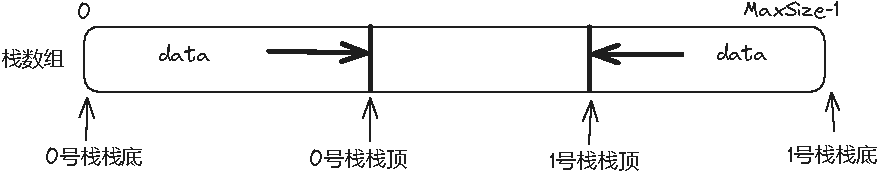
\includegraphics[width=1\textwidth]{./figure/pdf/cropped/shareStack.pdf}
  \caption{共享栈}
  \label{fig:sharedStack}
\end{figure}


共享栈的结构体定义如代码\ref{lst:sharedStackStruct}所示。

\begin{lstlisting}[language=C++, caption={共享栈结构体定义}, label={lst:sharedStackStruct}]
  struct SharedStack {
    int* data;//栈的数据元素
    int top1;//栈1的栈顶指针
    int top2;//栈2的栈顶指针
    int capacity;//栈的容量
  };
\end{lstlisting}

共享栈的基本操作包括创建、销毁、压入、弹出、获取栈顶元素、判断栈是否为空、判断栈是否为满、获取栈的大小和获取栈的容量。

\textbf{创建操作}:

创建一个空共享栈,需要为栈分配内存空间,并初始化栈的大小、栈的容量和栈顶指针。

代码如代码\ref{lst:createSharedStack}所示。

\begin{lstlisting}[language=C++, caption={创建一个空共享栈示例代码}, label={lst:createSharedStack}]
  SharedStack* createSharedStack(int capacity) {
    SharedStack* S = (SharedStack*)malloc(sizeof(SharedStack));
    S->data = (int*)malloc(sizeof(int) * capacity);
    S->top1 = -1;
    S->top2 = capacity;
    S->capacity = capacity;
    return S;
  }

\end{lstlisting}

该算法的总时间复杂度为 $O(1)$,空间复杂度为 $O(1)$。

特点:创建的共享栈为空,不包含任何数据元素。

\textbf{销毁操作}:

销毁共享栈,需要释放栈的内存空间。

代码如代码\ref{lst:destroySharedStack}所示。

\begin{lstlisting}[language=C++, caption={销毁共享栈示例代码}, label={lst:destroySharedStack}]
  void destroySharedStack(SharedStack* S) {
    free(S->data);
    free(S);
  }

\end{lstlisting}

该算法的总时间复杂度为 $O(1)$,空间复杂度为 $O(1)$。

特点:销毁共享栈,释放栈的内存空间。

\textbf{判空操作}:

判断共享栈是否为空,即栈中不包含任何元素。

代码如代码\ref{lst:isEmptySharedStack}所示。

\begin{lstlisting}[language=C++, caption={判断共享栈是否为空示例代码}, label={lst:isEmptySharedStack}]
  bool isEmptySharedStack(SharedStack* S, int stackNumber) {
    if (stackNumber == 1) {
      return S->top1 == -1;
    } else if (stackNumber == 2) {
      return S->top2 == S->capacity;
    } else {
      return false;
    }
  }

\end{lstlisting}

该算法的总时间复杂度为 $O(1)$,空间复杂度为 $O(1)$。

特点:判断共享栈是否为空,即栈中不包含任何元素。

\textbf{判满操作}:

判断共享栈是否为满,即栈中包含的元素个数等于栈的容量。

代码如代码\ref{lst:isFullSharedStack}所示。

\begin{lstlisting}[language=C++, caption={判断共享栈是否为满示例代码}, label={lst:isFullSharedStack}]
  bool isFullSharedStack(SharedStack* S) {
    return S->top1 + 1 == S->top2;
  }

\end{lstlisting}

该算法的总时间复杂度为 $O(1)$,空间复杂度为 $O(1)$。

特点:判断共享栈是否为满,即栈中包含的元素个数等于栈的容量。

\textbf{压入操作}:

将元素压入共享栈中,即将元素放入栈顶。

代码如代码\ref{lst:pushSharedStack}所示。

\begin{lstlisting}[language=C++, caption={压入共享栈示例代码}, label={lst:pushSharedStack}]
  void pushSharedStack(SharedStack* S, int data, int stackNumber) {
    if (isFullSharedStack(S)) {
      printf(``栈已满,无法压入元素\n``);
      return;
    }
    if (stackNumber == 1) {
      S->data[++S->top1] = data;
    } else if (stackNumber == 2) {
      S->data[--S->top2] = data;
    }
  }

\end{lstlisting}

该算法的总时间复杂度为 $O(1)$,空间复杂度为 $O(1)$。

特点:将元素压入共享栈中,即将元素放入栈顶。

\textbf{弹出操作}:

将元素从共享栈中弹出,即将栈顶元素删除。

代码如代码\ref{lst:popSharedStack}所示。

\begin{lstlisting}[language=C++, caption={弹出共享栈示例代码}, label={lst:popSharedStack}]
  void popSharedStack(SharedStack* S, int stackNumber) {
    if (isEmptySharedStack(S, stackNumber)) {
      printf(``栈为空,无法弹出元素\n``);
      return;
    }
    if (stackNumber == 1) {
      S->top1--;
    } else if (stackNumber == 2) {
      S->top2++;
    }
  }

\end{lstlisting}

该算法的总时间复杂度为 $O(1)$,空间复杂度为 $O(1)$。

特点:将元素从共享栈中弹出,即将栈顶元素删除。

\textbf{获取栈顶元素}:

获取共享栈的栈顶元素,即获取栈顶元素的值。

代码如代码\ref{lst:getTopSharedStack}所示。

\begin{lstlisting}[language=C++, caption={获取共享栈的栈顶元素示例代码}, label={lst:getTopSharedStack}]
  int getTopSharedStack(SharedStack* S, int stackNumber) {
    if (isEmptySharedStack(S, stackNumber)) {
      printf(``栈为空,无法获取栈顶元素\n``);
      return -1;
    }
    if (stackNumber == 1) {
      return S->data[S->top1];
    } else if (stackNumber == 2) {
      return S->data[S->top2];
    } else {
      return -1;
    }
  }

\end{lstlisting}

该算法的总时间复杂度为 $O(1)$,空间复杂度为 $O(1)$。

特点:获取共享栈的栈顶元素,即获取栈顶元素的值。

\textbf{获取栈的大小}:

获取共享栈的大小,即获取栈中包含的元素个数。

代码如代码\ref{lst:sizeSharedStack}所示。

\begin{lstlisting}[language=C++, caption={获取共享栈的大小示例代码}, label={lst:sizeSharedStack}]
  int sizeSharedStack(SharedStack* S) {
    return S->top1 + 1 + S->capacity - S->top2;
  }

\end{lstlisting}

该算法的总时间复杂度为 $O(1)$,空间复杂度为 $O(1)$。

特点:获取共享栈的大小,即获取栈中包含的元素个数。

\textbf{获取栈的容量}:

获取共享栈的容量,即获取栈的最大容量。

代码如代码\ref{lst:capacitySharedStack}所示。

\begin{lstlisting}[language=C++, caption={获取共享栈的容量示例代码}, label={lst:capacitySharedStack}]
  int capacitySharedStack(SharedStack* S) {
    return S->capacity;
  }

\end{lstlisting}

该算法的总时间复杂度为 $O(1)$,空间复杂度为 $O(1)$。

特点:获取共享栈的容量,即获取栈的最大容量。

\textbf{清空栈}:

清空共享栈,即将栈中的所有元素删除。

代码如代码\ref{lst:clearSharedStack}所示。

\begin{lstlisting}[language=C++, caption={清空共享栈示例代码}, label={lst:clearSharedStack}]
  void clearSharedStack(SharedStack* S) {
    S->top1 = -1;
    S->top2 = S->capacity;
  }

\end{lstlisting}

该算法的总时间复杂度为 $O(1)$,空间复杂度为 $O(1)$。

特点:清空共享栈,即将栈中的所有元素删除。

\textbf{遍历栈}:

遍历共享栈,即输出栈中的所有元素。

代码如代码\ref{lst:traverseSharedStack}所示。

\begin{lstlisting}[language=C++, caption={遍历共享栈示例代码}, label={lst:traverseSharedStack}]
  void traverseSharedStack(SharedStack* S) {
    for (int i = 0; i <= S->top1; i++) {
      printf(``%d ``, S->data[i]);
    }
    for (int i = S->capacity - 1; i >= S->top2; i--) {
      printf(``%d ``, S->data[i]);
    }
    printf(``\n``);
  }

\end{lstlisting}

该算法的总时间复杂度为 $O(n)$,空间复杂度为 $O(1)$。

特点:遍历共享栈,即输出栈中的所有元素。


\section{队列}



\subsection{队列的定义}

队列是一种先进先出的线性表,只允许在表的一端进行插入,而在另一端进行删除操作。


\subsection{队列的操作}

队列的基本操作包括创建、销毁、入队、出队、获取队头元素、判断队列是否为空、判断队列是否为满、获取队列的大小和获取队列的容量。


\subsection{顺序队列}

顺序队列是使用数组实现的队列,队列的大小是固定的,队列的容量是数组的大小。

顺序队列的结构如如图\ref{fig:seqQueue}所示。

\begin{figure}[!htbp]
  \centering
  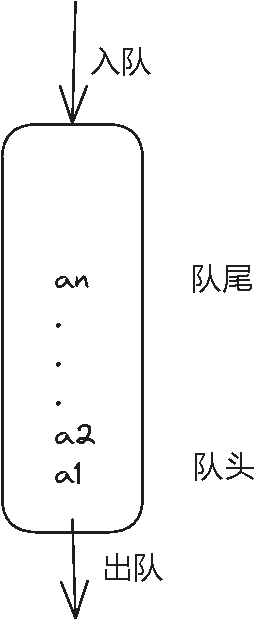
\includegraphics[width=0.1\textwidth]{./figure/pdf/cropped/seqQueue.pdf}
  \caption{顺序队列}
  \label{fig:seqQueue}
\end{figure}

顺序队列的结构体定义如代码\ref{lst:seqQueueStruct}所示。

\begin{lstlisting}[language=C++, caption={顺序队列结构体定义}, label={lst:seqQueueStruct}]
  struct SeqQueue {
    int* data;//队列的数据元素
    int front;//队头指针
    int rear;//队尾指针
    int capacity;//队列的容量
  };
\end{lstlisting}


顺序队列的存放过程如图\ref{fig:seqQueuePut}所示。

\begin{figure}[!htbp]
  \centering
  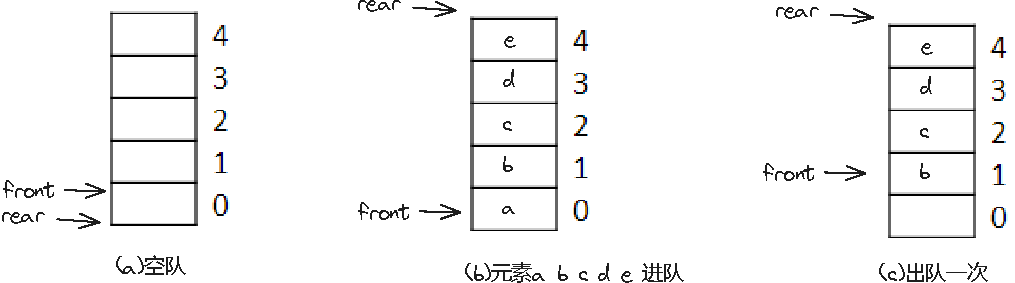
\includegraphics[width=1\textwidth]{./figure/pdf/cropped/seqQueuePut.pdf}
  \caption{顺序队列的存放过程}
  \label{fig:seqQueuePut}
\end{figure}

相关术语:

\begin{itemize}
  \item 队头指针:指向队头元素的前一个位置。
  \item 队尾指针:指向队尾元素。
  \item 队列的容量:队列的最大容量。
  \item 队列的大小:队列中包含的元素个数。
  \item 队列的长度:队列中包含的元素个数。
  \item 队列的空间:队列的容量减去队列的大小。
  \item 队列的空:队列的大小为0。
  \item 队列的满:队列的大小等于队列的容量。
\end{itemize}

顺序队列的基本操作包括创建、销毁、入队、出队、获取队头元素、判断队列是否为空、判断队列是否为满、获取队列的大小和获取队列的容量。

\textbf{创建操作}:

创建一个空顺序队列,需要为队列分配内存空间,并初始化队头指针、队尾指针和队列的容量。

代码如代码\ref{lst:createSeqQueue}所示。

\begin{lstlisting}[language=C++, caption={创建一个空顺序队列示例代码}, label={lst:createSeqQueue}]
  SeqQueue* createSeqQueue(int capacity) {
    SeqQueue* Q = (SeqQueue*)malloc(sizeof(SeqQueue));
    Q->data = (int*)malloc(sizeof(int) * capacity);
    Q->front = 0;
    Q->rear = 0;
    Q->capacity = capacity;
    return Q;
  }

\end{lstlisting}

该算法的总时间复杂度为 $O(1)$,空间复杂度为 $O(1)$。

特点:创建的顺序队列为空,不包含任何数据元素。

\textbf{销毁操作}:

销毁顺序队列,需要释放队列的内存空间。

代码如代码\ref{lst:destroySeqQueue}所示。

\begin{lstlisting}[language=C++, caption={销毁顺序队列示例代码}, label={lst:destroySeqQueue}]
  void destroySeqQueue(SeqQueue* Q) {
    free(Q->data);
    free(Q);
  }

\end{lstlisting}

该算法的总时间复杂度为 $O(1)$,空间复杂度为 $O(1)$。

特点:销毁顺序队列,释放队列的内存空间。

\textbf{判空操作}:

判断顺序队列是否为空,即队列中不包含任何元素。

代码如代码\ref{lst:isEmptySeqQueue}所示。

\begin{lstlisting}[language=C++, caption={判断顺序队列是否为空示例代码}, label={lst:isEmptySeqQueue}]
  bool isEmptySeqQueue(SeqQueue* Q) {
    return Q->front == Q->rear;
  }

\end{lstlisting}

该算法的总时间复杂度为 $O(1)$,空间复杂度为 $O(1)$。

特点:判断顺序队列是否为空,即队列中不包含任何元素。

\textbf{判满操作}:

判断顺序队列是否为满,即队列中包含的元素个数等于队列的容量。

代码如代码\ref{lst:isFullSeqQueue}所示。

\begin{lstlisting}[language=C++, caption={判断顺序队列是否为满示例代码}, label={lst:isFullSeqQueue}]
  bool isFullSeqQueue(SeqQueue* Q) {
    return (Q->rear + 1) % Q->capacity == Q->front;
  }

\end{lstlisting}

该算法的总时间复杂度为 $O(1)$,空间复杂度为 $O(1)$。

特点:判断顺序队列是否为满,即队列中包含的元素个数等于队列的容量。

\textbf{入队操作}:

将元素入队,即将元素放入队尾。

代码如代码\ref{lst:enQueueSeqQueue}所示。

\begin{lstlisting}[language=C++, caption={入队示例代码}, label={lst:enQueueSeqQueue}]
  void enQueueSeqQueue(SeqQueue* Q, int data) {
    if (isFullSeqQueue(Q)) {
      printf(``队列已满,无法入队\n``);
      return;
    }
    Q->data[Q->rear] = data;
    Q->rear = (Q->rear + 1) % Q->capacity;
  }

\end{lstlisting}

该算法的总时间复杂度为 $O(1)$,空间复杂度为 $O(1)$。

特点:将元素入队,即将元素放入队尾。

\textbf{出队操作}:

将元素出队,即将队头元素删除。

代码如代码\ref{lst:deQueueSeqQueue}所示。

\begin{lstlisting}[language=C++, caption={出队示例代码}, label={lst:deQueueSeqQueue}]
  void deQueueSeqQueue(SeqQueue* Q) {
    if (isEmptySeqQueue(Q)) {
      printf(``队列为空,无法出队\n``);
      return;
    }
    Q->front = (Q->front + 1) % Q->capacity;
  }

\end{lstlisting}

该算法的总时间复杂度为 $O(1)$,空间复杂度为 $O(1)$。

特点:将元素出队,即将队头元素删除。

\textbf{获取队头元素}:

获取顺序队列的队头元素,即获取队头元素的值。

代码如代码\ref{lst:getFrontSeqQueue}所示。

\begin{lstlisting}[language=C++, caption={获取队头元素示例代码}, label={lst:getFrontSeqQueue}]
  int getFrontSeqQueue(SeqQueue* Q) {
    if (isEmptySeqQueue(Q)) {
      printf(``队列为空,无法获取队头元素\n``);
      return -1;
    }
    return Q->data[Q->front];
  }

\end{lstlisting}

该算法的总时间复杂度为 $O(1)$,空间复杂度为 $O(1)$。

特点:获取顺序队列的队头元素,即获取队头元素的值。

\textbf{获取队列的大小}:

获取顺序队列的大小,即获取队列中包含的元素个数。

代码如代码\ref{lst:sizeSeqQueue}所示。

\begin{lstlisting}[language=C++, caption={获取队列的大小示例代码}, label={lst:sizeSeqQueue}]
  int sizeSeqQueue(SeqQueue* Q) {
    return (Q->rear - Q->front + Q->capacity) % Q->capacity;
  }

\end{lstlisting}

该算法的总时间复杂度为 $O(1)$,空间复杂度为 $O(1)$。

特点:获取顺序队列的大小,即获取队列中包含的元素个数。

\textbf{获取队列的容量}:

获取顺序队列的容量,即获取队列的最大容量。

代码如代码\ref{lst:capacitySeqQueue}所示。

\begin{lstlisting}[language=C++, caption={获取队列的容量示例代码}, label={lst:capacitySeqQueue}]
  int capacitySeqQueue(SeqQueue* Q) {
    return Q->capacity;
  }

\end{lstlisting}

该算法的总时间复杂度为 $O(1)$,空间复杂度为 $O(1)$。

特点:获取顺序队列的容量,即获取队列的最大容量。

\textbf{清空队列}:

清空顺序队列,即将队列中的所有元素删除。

代码如代码\ref{lst:clearSeqQueue}所示。

\begin{lstlisting}[language=C++, caption={清空队列示例代码}, label={lst:clearSeqQueue}]
  void clearSeqQueue(SeqQueue* Q) {
    Q->front = 0;
    Q->rear = 0;
  }

\end{lstlisting}

该算法的总时间复杂度为 $O(1)$,空间复杂度为 $O(1)$。

特点:清空顺序队列,即将队列中的所有元素删除。

\textbf{遍历队列}:

遍历顺序队列,即输出队列中的所有元素。

代码如代码\ref{lst:traverseSeqQueue}所示。

\begin{lstlisting}[language=C++, caption={遍历队列示例代码}, label={lst:traverseSeqQueue}]
  void traverseSeqQueue(SeqQueue* Q) {
    for (int i = Q->front; i != Q->rear; i = (i + 1) % Q->capacity) {
      printf(``%d ``, Q->data[i]);
    }
    printf(``\n``);
  }

\end{lstlisting}

该算法的总时间复杂度为 $O(n)$,空间复杂度为 $O(1)$。

特点:遍历顺序队列,即输出队列中的所有元素。

针对循环队列,我们还可以使用另外两种方法来判断队列是否为空和队列是否为满。

第一种:使用一个变量记录队列的大小,当队列为空时,队列的大小为0;当队列为满时,队列的大小等于队列的容量。

第二种:新增一个tag变量,当队列为空时,tag等于0;当队列为满时,tag等于1。
第一种的结构体为:

\begin{lstlisting}[language=C++, caption={循环队列结构体定义}, label={lst:circleQueueStruct}]
  struct CircleQueue {
    int* data;//队列的数据元素
    int front;//队头指针
    int rear;//队尾指针
    int capacity;//队列的容量
  };
\end{lstlisting}

\textbf{判空操作}:

判断循环队列是否为空,即队列中不包含任何元素。

代码如代码\ref{lst:isEmptyCircleQueue}所示。

\begin{lstlisting}[language=C++, caption={判断循环队列是否为空示例代码}, label={lst:isEmptyCircleQueue}]
  bool isEmptyCircleQueue(CircleQueue* Q) {
    return Q->front == Q->rear;
  }

\end{lstlisting}

\textbf{判满操作}:

判断循环队列是否为满,即队列中包含的元素个数等于队列的容量。

代码如代码\ref{lst:isFullCircleQueue}所示。

\begin{lstlisting}[language=C++, caption={判断循环队列是否为满示例代码}, label={lst:isFullCircleQueue}]
  bool isFullCircleQueue(CircleQueue* Q) {
    return (Q->rear + 1) % Q->capacity == Q->front;
  }

\end{lstlisting}

第二种的结构体为:

\begin{lstlisting}[language=C++, caption={循环队列结构体定义}, label={lst:circleQueueStruct2}]
  struct CircleQueue {
    int* data;//队列的数据元素
    int front;//队头指针
    int rear;//队尾指针
    int tag;//标记队列是否为满
    int capacity;//队列的容量
  };
\end{lstlisting}

\textbf{判空操作}:

判断循环队列是否为空,即队列中不包含任何元素。

代码如代码\ref{lst:isEmptyCircleQueue2}所示。

\begin{lstlisting}[language=C++, caption={判断循环队列是否为空示例代码}, label={lst:isEmptyCircleQueue2}]
  bool isEmptyCircleQueue(CircleQueue* Q) {
    return Q->front == Q->rear && Q->tag == 0;
  }

\end{lstlisting}

\textbf{判满操作}:

判断循环队列是否为满,即队列中包含的元素个数等于队列的容量。

代码如代码\ref{lst:isFullCircleQueue2}所示。

\begin{lstlisting}[language=C++, caption={判断循环队列是否为满示例代码}, label={lst:isFullCircleQueue2}]
  bool isFullCircleQueue(CircleQueue* Q) {
    return Q->front == Q->rear && Q->tag == 1;
  }

\end{lstlisting}

\subsection{链式队列}

链式队列是使用链表实现的队列,队列的大小是动态的,队列的容量是无限的。

链式队列的结构如如图\ref{fig:linkQueue}所示。

\begin{figure}[!htbp]
  \centering
  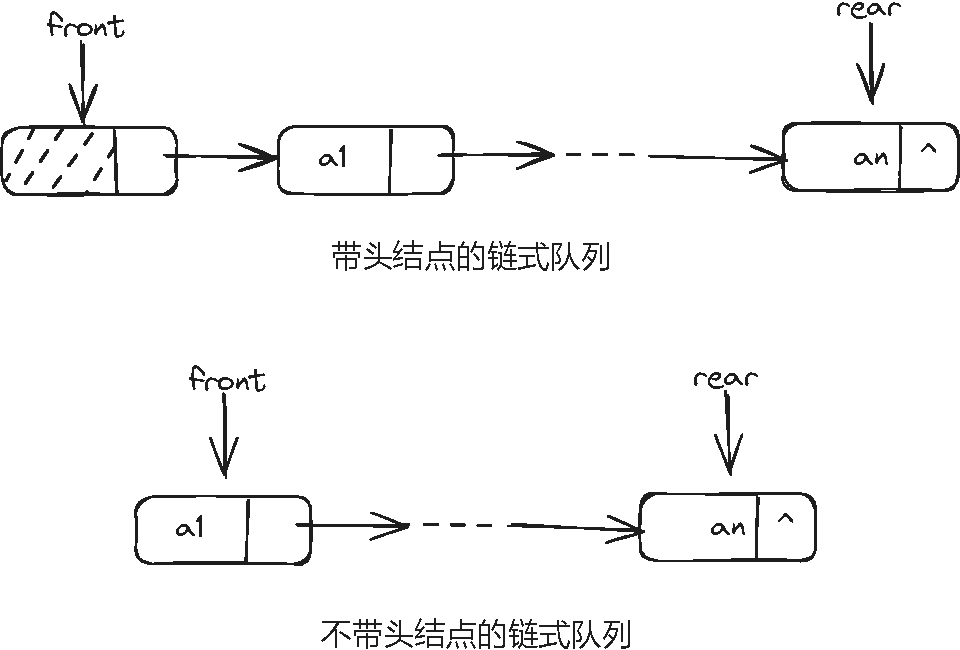
\includegraphics[width=1\textwidth]{./figure/pdf/cropped/linkQueue.pdf}
  \caption{链式队列}
  \label{fig:linkQueue}
\end{figure}

图中示出了两类链式队列,一类带头结点,一类不带头结点。

我们可以发现,不带头结点的链式队列需要特殊处理队列为空的情况,因为队列为空时,
队头指针和队尾指针都为空。因此,我们通常使用带头结点的链式队列。

链式队列的结构体定义如代码\ref{lst:linkQueueStruct}所示。

\begin{lstlisting}[language=C++, caption={链式队列结构体定义}, label={lst:linkQueueStruct}]
  struct singleLink {
	NODETYPE data;
	singleLink* next;
  }; 
  struct LinkQueue {
    singleLink* front, * rear;
  };
\end{lstlisting}

链式队列的基本操作包括创建、销毁、入队、出队、获取队头元素、判断队列是否为空、获取队列的大小。

\textbf{创建操作}:

创建一个空链式队列,需要为队列分配内存空间,并初始化队头指针和队尾指针。

代码如代码\ref{lst:createLinkQueue}所示。

\begin{lstlisting}[language=C++, caption={创建一个空链式队列示例代码}, label={lst:createLinkQueue}]
  LinkQueue* createLinkQueue() {
    singleLink* h = (singleLink*)malloc(sizeof(singleLink));
    LinkQueue* Q = (LinkQueue*)malloc(sizeof(LinkQueue));
    Q->front = h;
    Q->rear = h;
    return Q;
  }
  \end{lstlisting}

该算法的总时间复杂度为 $O(1)$,空间复杂度为 $O(1)$。

特点:创建的链式队列为空,不包含任何数据元素。

\textbf{销毁操作}:

销毁链式队列,需要释放队列的内存空间。

代码如代码\ref{lst:destroyLinkQueue}所示。

\begin{lstlisting}[language=C++, caption={销毁链式队列示例代码}, label={lst:destroyLinkQueue}]
  void destroyLinkQueue(LinkQueue* Q) {
    singleLink* p = Q->front;
    while (p != NULL) {
      singleLink* q = p;
      p = p->next;
      free(q);
    }
    free(Q);
  }

\end{lstlisting}

该算法的总时间复杂度为 $O(n)$,空间复杂度为 $O(1)$。

特点:销毁链式队列,释放队列的内存空间。

\textbf{判空操作}:

判断链式队列是否为空,即队列中不包含任何元素。

代码如代码\ref{lst:isEmptyLinkQueue}所示。

\begin{lstlisting}[language=C++, caption={判断链式队列是否为空示例代码}, label={lst:isEmptyLinkQueue}]
  bool isEmptyLinkQueue(LinkQueue* Q) {
    return Q->front == Q->rear;
  }

\end{lstlisting}

该算法的总时间复杂度为 $O(1)$,空间复杂度为 $O(1)$。

特点:判断链式队列是否为空,即队列中不包含任何元素。

\textbf{入队操作}:

将元素入队,即将元素放入队尾。

代码如代码\ref{lst:enQueueLinkQueue}所示。

\begin{lstlisting}[language=C++, caption={入队示例代码}, label={lst:enQueueLinkQueue}]
  void enQueueLinkQueue(LinkQueue* Q, NODETYPE data) {
    singleLink* p = (singleLink*)malloc(sizeof(singleLink));
    p->data = data;
    p->next = NULL;
    Q->rear->next = p;
    Q->rear = p;
  }

\end{lstlisting}

该算法的总时间复杂度为 $O(1)$,空间复杂度为 $O(1)$。

特点:将元素入队,即将元素放入队尾。

\textbf{出队操作}:

将元素出队,即将队头元素删除。

代码如代码\ref{lst:deQueueLinkQueue}所示。

\begin{lstlisting}[language=C++, caption={出队示例代码}, label={lst:deQueueLinkQueue}]
  void deQueueLinkQueue(LinkQueue* Q) {
    if (isEmptyLinkQueue(Q)) {
      printf(``队列为空,无法出队\n``);
      return;
    }
    singleLink* p = Q->front->next;
    Q->front->next = p->next;
    if (Q->rear == p) {
      Q->rear = Q->front;
    }
    free(p);
  }

\end{lstlisting}

该算法的总时间复杂度为 $O(1)$,空间复杂度为 $O(1)$。

特点:将元素出队,即将队头元素删除。

\textbf{获取队头元素}:

获取链式队列的队头元素,即获取队头元素的值。

代码如代码\ref{lst:getFrontLinkQueue}所示。

\begin{lstlisting}[language=C++, caption={获取队头元素示例代码}, label={lst:getFrontLinkQueue}]
  NODETYPE getFrontLinkQueue(LinkQueue* Q) {
    if (isEmptyLinkQueue(Q)) {
      printf(``队列为空,无法获取队头元素\n``);
      return -1;
    }
    return Q->front->next->data;
  }

\end{lstlisting}

该算法的总时间复杂度为 $O(1)$,空间复杂度为 $O(1)$。

特点:获取链式队列的队头元素,即获取队头元素的值。

\textbf{获取队列的大小}:

获取链式队列的大小,即获取队列中包含的元素个数。

代码如代码\ref{lst:sizeLinkQueue}所示。

\begin{lstlisting}[language=C++, caption={获取队列的大小示例代码}, label={lst:sizeLinkQueue}]
  int sizeLinkQueue(LinkQueue* Q) {
    int size = 0;
    singleLink* p = Q->front->next;
    while (p != NULL) {
      size++;
      p = p->next;
    }
    return size;
  }

\end{lstlisting}

该算法的总时间复杂度为 $O(n)$,空间复杂度为 $O(1)$。

特点:获取链式队列的大小,即获取队列中包含的元素个数。

\textbf{清空队列}:

清空链式队列,即将队列中的所有元素删除。

代码如代码\ref{lst:clearLinkQueue}所示。

\begin{lstlisting}[language=C++, caption={清空队列示例代码}, label={lst:clearLinkQueue}]
  void clearLinkQueue(LinkQueue* Q) {
    singleLink* p = Q->front->next;
    while (p != NULL) {
      singleLink* q = p;
      p = p->next;
      free(q);
    }
    Q->rear = Q->front;
  }

\end{lstlisting}

该算法的总时间复杂度为 $O(n)$,空间复杂度为 $O(1)$。

特点:清空链式队列,即将队列中的所有元素删除。

\textbf{遍历队列}:

遍历链式队列,即输出队列中的所有元素。

代码如代码\ref{lst:traverseLinkQueue}所示。

\begin{lstlisting}[language=C++, caption={遍历队列示例代码}, label={lst:traverseLinkQueue}]
  void traverseLinkQueue(LinkQueue* Q) {
    singleLink* p = Q->front->next;
    while (p != NULL) {
      printf(``%d ``, p->data);
      p = p->next;
    }
    printf(``\n``);
  }

\end{lstlisting}

该算法的总时间复杂度为 $O(n)$,空间复杂度为 $O(1)$。

特点:遍历链式队列,即输出队列中的所有元素。





\subsection{双端队列}

双端队列是一种具有队列和栈的性质的线性表,双端队列的两端都可以进行插入和删除操作。

双端队列的结构如如图\ref{fig:deque}所示。

\begin{figure}[!htbp]
  \centering
  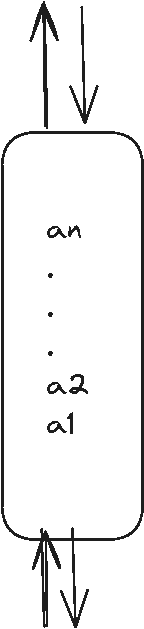
\includegraphics[width=0.1\textwidth]{./figure/pdf/cropped/DQueue.pdf}
  \caption{双端队列}
  \label{fig:deque}
\end{figure}


\section{栈和队列的应用}

\subsection{栈的应用}

\subsubsection{简单表达式求值}

这里限定的简单表达式是用户输入的一个包含+、-、*、/、(、)和正整数的合法算数表达式,计算该表达式的运算结果。

在算术表达式中, 运算符位于两个操作数中间的表达式称为中缀表达式 (infix
expression) ,例如 1+2*3 就是一个中缀表达式。中缀表达式是一种最常用的表达式形式,
日常生活中的表达式一般都是中缀表达式。

中缀表达式的运算一般遵循“先乘除,后加减,从左到右计算,先括号内,后括号外的
规则,因此中缀表达式不仅要依赖运算符优先级,还要处理括号。

算术表达式的另一种形式是后缀表达式(postfix expression)或逆波兰表达式,就是在
算术表达式中运算符在操作数的后面,如1 + 2 * 3 的后组表达式为 1 2 3 * +。在后缀表
达式中已经考虑了运算符的优先级,没有括号,只有操作数和运算符,而且越放在前面的运
算符越优先执行。

同样,在算术表达式中,如果运算符在操作数的前面,称为前缀表达式 (prefix
expression) ,如 1 + 2 * 3 的前缀表达式为+ 1 * 2 3。

后缀表达式是一种十分有用的表达式,它将复杂表达式转换为可以依靠简单的操作得
到计算结果的表达式。所以对中缀表达式的求值过程是先将中缀算术表达式转换成后缀表
达式,然后对该后缀表达式求值。


\textbf{中缀表达式转后缀表达式}

中缀表达式转后缀表达式的算法如下:

1. 从左到右扫描中缀表达式。

2. 如果是操作数,则直接输出。

3. 如果是运算符,则判断其与栈顶运算符的优先级,是右括号或优先级低于栈顶运算符,则栈顶运算符依次出栈并输出,直到遇到左括号或栈空为止。此时将当前运算符入栈。

4. 如果是左括号,则直接入栈。

5. 如果是右括号,则依次出栈并输出直到遇到左括号,左括号出栈。

6. 重复2-5步骤,直到表达式的最右端。

7. 将栈中的运算符依次出栈并输出。

例如,中缀表达式$3+5*8-(6 + 2)$转换为后缀表达式的过程如表\ref{tab:infixToPostfix}所示。


\begin{table}[!htbp]
  \centering
  \begin{tabular}{|c|c|c|}
  \hline
  \textbf{扫描的符号} & \textbf{栈 (Stack)} & \textbf{输出 (Output)} \\ \hline
  3 &  & 3 \\ \hline
  + & + & 3 \\ \hline
  5 & + & 3 5 \\ \hline
  * & + * & 3 5 \\ \hline
  8 & + * & 3 5 8 \\ \hline
  - & - & 3 5 8 * + \\ \hline
  ( & - ( & 3 5 8 * + \\ \hline
  6 & - ( & 3 5 8 * + 6 \\ \hline
  + & - ( + & 3 5 8 * + 6 \\ \hline
  2 & - ( + & 3 5 8 * + 6 2 \\ \hline
  ) & - & 3 5 8 * + 6 2 + \\ \hline
  (结束) &  & 3 5 8 * + 6 2 + - \\ \hline
  \end{tabular}
  \caption{前缀转后缀}
  \label{tab:infixToPostfix}
  \end{table}

代码如代码\ref{lst:infixToPostfix}所示。

\begin{lstlisting}[language=C++, caption={中缀表达式转后缀表达式示例代码}, label={lst:infixToPostfix}]
  bool isOperator(char c) {
    return c == '+' || c == '-' || c == '*' || c == '/';
  }

  int priority(char c) {
    if (c == '+' || c == '-') {
      return 1;
    }
    if (c == '*' || c == '/') {
      return 2;
    }
    return 0;
  }

  string infixToPostfix(string infix) {
    stack<char> s;
    string postfix = ````;
    for (int i = 0; i < infix.size(); i++) {
      if (isdigit(infix[i])) {
        postfix += infix[i];
      } else if (infix[i] == '(') {
        s.push(infix[i]);
      } else if (infix[i] == ')') {
        while (!s.empty() && s.top() != '(') {
          postfix += s.top();
          s.pop();
        }
        s.pop();
      } else if (isOperator(infix[i])) {
        while (!s.empty() && priority(s.top()) >= priority(infix[i])) {
          postfix += s.top();
          s.pop();
        }
        s.push(infix[i]);
      }
    }
    while (!s.empty()) {
      postfix += s.top();
      s.pop();
    }
    return postfix;
  }

\end{lstlisting}

该算法的总时间复杂度为 $O(n)$,空间复杂度为 $O(n)$。

特点:中缀表达式转后缀表达式。

\textbf{后缀表达式求值}

后缀表达式求值的算法如下:

1. 从左到右扫描后缀表达式。

2. 如果是操作数,则入栈。

3. 如果是运算符,则从栈中弹出两个操作数,进行运算,将运算结果入栈。

4. 重复2-3步骤,直到表达式的最右端。

5. 栈中的元素即为表达式的运算结果。

例如,后缀表达式$3 5 8 * + 6 2 + -$的求值过程如表\ref{tab:postfixEvaluation}所示。

\begin{table}[!htbp]
  \centering
  \begin{tabular}{|c|c|}
  \hline
  \textbf{扫描的符号} & \textbf{栈 (Stack)} \\ \hline
  3 & 3 \\ \hline
  5 & 3 5 \\ \hline
  8 & 3 5 8 \\ \hline
  * & 3 40 \\ \hline
  + & 43 \\ \hline
  6 & 43 6 \\ \hline
  2 & 43 6 2 \\ \hline
  + & 43 8 \\ \hline
  - & 35 \\ \hline
  \end{tabular}
  \caption{后缀表达式求值}
  \label{tab:postfixEvaluation}
  \end{table}

代码如代码\ref{lst:postfixEvaluation}所示。

\begin{lstlisting}[language=C++, caption={后缀表达式求值示例代码}, label={lst:postfixEvaluation}]
  int postfixEvaluation(string postfix) {
    stack<int> s;
    for (int i = 0; i < postfix.size(); i++) {
      if (isdigit(postfix[i])) {
        s.push(postfix[i] - '0');
      } else {
        int b = s.top();
        s.pop();
        int a = s.top();
        s.pop();
        if (postfix[i] == '+') {
          s.push(a + b);
        } else if (postfix[i] == '-') {
          s.push(a - b);
        } else if (postfix[i] == '*') {
          s.push(a * b);
        } else if (postfix[i] == '/') {
          s.push(a / b);
        }
      }
    }
    return s.top();
  }

\end{lstlisting}


\subsubsection{括号匹配}

括号匹配是指对于一个字符串,其中包含的括号必须是成对出现的,且左括号必须在右括号的前面。

例如,字符串“((()))”是括号匹配的,而字符串“(()))”不是括号匹配的。

括号匹配的算法如下:

1. 从左到右扫描字符串。

2. 如果是左括号,则入栈。

3. 如果是右括号,则判断栈是否为空,如果为空,则返回false;否则,出栈。

4. 重复2-3步骤,直到字符串的最右端。

5. 如果栈为空,则返回true;否则,返回false。

例如,字符串“(())()”的括号匹配过程如表\ref{tab:bracketMatching}所示。

\begin{table}[!htbp]
  \centering
  \begin{tabular}{|c|c|c|}
  \hline
  \textbf{扫描的符号} & \textbf{栈 (Stack)} & \textbf{是否匹配} \\ \hline
  ( & ( &  \\ \hline
  ( & (( &  \\ \hline
  ) & ( &  \\ \hline
  ) &  &  \\ \hline
  ( & ( &  \\ \hline
  ) &  &  \\ \hline
  (结束) &  & 是 \\ \hline
  \end{tabular}
  \caption{括号匹配}
  \label{tab:bracketMatching}
  \end{table}

代码如代码\ref{lst:bracketMatching}所示。

\begin{lstlisting}[language=C++, caption={括号匹配示例代码}, label={lst:bracketMatching}]
  bool bracketMatching(string s) {
    stack<char> st;
    for (int i = 0; i < s.size(); i++) {
      if (s[i] == '(') {
        st.push(s[i]);
      } else if (s[i] == ')') {
        if (st.empty()) {
          return false;
        }
        st.pop();
      }
    }
    return st.empty();
  }

\end{lstlisting}

该算法的总时间复杂度为 $O(n)$,空间复杂度为 $O(n)$。


\subsection{队列的应用}

\subsubsection{约瑟夫环问题}

约瑟夫环问题是一个著名的问题,是一个数学的应用问题,该问题的大致描述如下:

设有n个人围成一圈,从第一个人开始报数,报到m的人出列,然后从出列的下一个人开始重新报数,报到m的人出列,如此循环,直到所有的人都出列为止。

例如,当n=6,m=5时,出列的顺序为5、4、6、2、3、1。

约瑟夫环问题的算法如下:

1. 创建一个队列,将所有的人依次入队。

2. 从队头开始,依次出队,报数,如果报数为m,则出队;否则,重新入队。

3. 重复2步骤,直到队列为空。

例如,当n=6,m=5时,出列的顺序为5、4、6、2、3、1。

代码如代码\ref{lst:josephus}所示。

\begin{lstlisting}[language=C++, caption={约瑟夫环问题示例代码}, label={lst:josephus}]
  void josephus(int n, int m) {
    queue<int> q;
    for (int i = 1; i <= n; i++) {
      q.push(i);
    }
    while (!q.empty()) {
      for (int i = 1; i < m; i++) {
        q.push(q.front());
        q.pop();
      }
      cout << q.front() << `` ``;
      q.pop();
    }
  }

\end{lstlisting}

该算法的总时间复杂度为 $O(nm)$,空间复杂度为 $O(n)$。





\chapter{串}

串(string)是由零个或多个字符组成的有限序列。含零个字符的串称为空串,用多表
示。串中所含字符的个数称为该串的长度(或串长)。通常将一个串表示成``aa …a, 的形
式,其中最外边的双引号(或单引号)不是串的内容,它们是串的标志,用于将串与标识符(如
变量名等)加以区别。每个字符(即使是空格)都占用一个存储单元,不同的机器和编程语言对合法字符
(即允许使用的字符)有不同的规定。但在一般情况下,英文字母、数字(0,1,…,9)和常用的
标点符号以及空格符等都是合法的字符。

两个串相等当且仅当这两个串的长度相等并且各对应位置上的字符都
相同。一个串中任意个连续字符组成的序列称为该串的子串(substring),
例如串``abcde``的子串有``a``、``ab``、``abc``和``abcd``等。为了表述清楚,
在串中空格字符用“␣”符号表示,例如``a␣b``是一个长度为3的串,其中含有一个空格字符。空串是不包含任何字符的串,其长度为0,空串是任何串的子串。


\section{串的存储结构}

串的存储结构有两种,即顺序存储结构和链式存储结构。
\subsection{顺序存储结构}


顺序串中的字符被依次存放在一组连续的存储单元里。一般来说,一个字节(8 位)可
以表示一个字符(存放其 ASCII 码) 。而计算机内存是按字编址的,即以字为存储单位,一
个存储单元指的是一个字。而一个字可能包含多个字节,其所包含的字节数随机器而异。

顺序串的存储方式有两种: 一种是每个字只存一个字符,如图\ref{fig:seqString}所示(假设一个字包
含4个字节) ,这称为非紧缩格式(其存储密度小); 另一种是每个字存放多个字符,如图\ref{fig:tightSeqString}
所示 ,这称为紧缩格式(其存储密度大) 。在这两个图中,有阴影的字节为空闲部分。



\begin{figure}[!htbp]
  \centering
  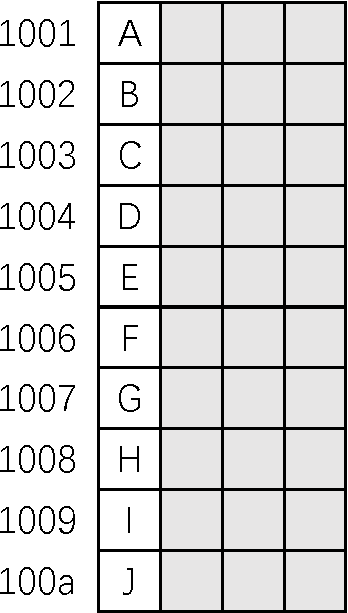
\includegraphics[width=0.2\textwidth]{./figure/pdf/cropped/narrowString.pdf}
  \caption{非紧缩格式的顺序串}
  \label{fig:seqString}
\end{figure}


\begin{figure}[!htbp]
  \centering
  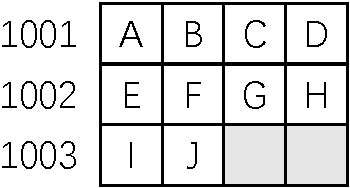
\includegraphics[width=0.2\textwidth]{./figure/pdf/cropped/notNarrowString.pdf}
  \caption{紧缩格式的顺序串}
  \label{fig:tightSeqString}
\end{figure}

串的紧缩格式存储方式是将串中的字符紧凑地存放在存储单元中,这样可以节省存储空间。
但是,在插入和删除操作时,需要移动大量的字符,因此效率较低。非紧缩格式存储方式是将 串中的字符依次存放在存储单元中,字符之间不留空,这样可以方便地进行插入和删除操作。
但是,由于字符之间没有留空,因此存储密度较低。
我们主要讨论非紧缩格式的顺序串。

顺序串的结构如代码\ref{lst:seqStringStruct}所示。

\begin{lstlisting}[language=C++, caption={顺序串结构体定义}, label={lst:seqStringStruct}]
  struct SeqString {
    char data[MAXSIZE];//存放串的字符数组
    int length;//串的长度
  };
\end{lstlisting}

顺序串的基本操作包括创建、销毁、清空、获取长度、获取字符、连接、比较、插入、删除、替换、复制、判断相等、求子串、输出等。

\textbf{创建操作}:

创建一个空串,需要为串分配内存空间,并初始化串的长度。

代码如代码\ref{lst:createSeqString}所示。

\begin{lstlisting}[language=C++, caption={创建一个空串示例代码}, label={lst:createSeqString}]
  SeqString* createSeqString() {
    SeqString* s = (SeqString*)malloc(sizeof(SeqString));
    s->length = 0;
    return s;
  }

\end{lstlisting}

该算法的总时间复杂度为 $O(1)$,空间复杂度为 $O(1)$。


\textbf{销毁操作}:

销毁串,需要释放串的内存空间。

代码如代码\ref{lst:destroySeqString}所示。

\begin{lstlisting}[language=C++, caption={销毁串示例代码}, label={lst:destroySeqString}]
  void destroySeqString(SeqString* s) {
    free(s);
  }

\end{lstlisting}

该算法的总时间复杂度为 $O(1)$,空间复杂度为 $O(1)$。


\textbf{清空操作}:

清空串,即将串的长度设置为0。

代码如代码\ref{lst:clearSeqString}所示。

\begin{lstlisting}[language=C++, caption={清空串示例代码}, label={lst:clearSeqString}]
  void clearSeqString(SeqString* s) {
    s->length = 0;
  }

\end{lstlisting}

该算法的总时间复杂度为 $O(1)$,空间复杂度为 $O(1)$。


\textbf{获取长度操作}:

获取串的长度。

代码如代码\ref{lst:lengthSeqString}所示。

\begin{lstlisting}[language=C++, caption={获取串的长度示例代码}, label={lst:lengthSeqString}]
  int lengthSeqString(SeqString* s) {
    return s->length;
  }

\end{lstlisting}

该算法的总时间复杂度为 $O(1)$,空间复杂度为 $O(1)$。


\textbf{获取字符操作}:

获取串中指定位置的字符。

代码如代码\ref{lst:getSeqString}所示。

\begin{lstlisting}[language=C++, caption={获取串中指定位置的字符示例代码}, label={lst:getSeqString}]
  char getSeqString(SeqString* s, int i) {
    if (i < 0 || i >= s->length) {
      printf(``位置不合法\n``);
      return -1;
    }
    return s->data[i];
  }

\end{lstlisting}

该算法的总时间复杂度为 $O(1)$,空间复杂度为 $O(1)$。


\textbf{连接操作}:

连接两个串,即将两个串连接成一个串。

代码如代码\ref{lst:concatSeqString}所示。

\begin{lstlisting}[language=C++, caption={连接两个串示例代码}, label={lst:concatSeqString}]
  SeqString* concatSeqString(SeqString* s1, SeqString* s2) {
    SeqString* s = createSeqString();
    for (int i = 0; i < s1->length; i++) {
      s->data[s->length++] = s1->data[i];
    }
    for (int i = 0; i < s2->length; i++) {
      s->data[s->length++] = s2->data[i];
    }
    return s;
  }

\end{lstlisting}

该算法的总时间复杂度为 $O(n)$,空间复杂度为 $O(n)$。


\textbf{比较操作}:

比较两个串的大小。

代码如代码\ref{lst:compareSeqString}所示。

\begin{lstlisting}[language=C++, caption={比较两个串的大小示例代码}, label={lst:compareSeqString}]
  int compareSeqString(SeqString* s1, SeqString* s2) {//s1>s2返回正数,s1=s2返回0,s1<s2返回负数
    int i = 0;
    while (i < s1->length && i < s2->length) {//比较两个串的公共部分
      if (s1->data[i] != s2->data[i]) {//如果两个串的字符不相等
        return s1->data[i] - s2->data[i];
      }
      i++;
    }
    return s1->length - s2->length;
  }

\end{lstlisting}

该算法的总时间复杂度为 $O(n)$,空间复杂度为 $O(1)$。


\textbf{插入操作}:

在指定位置插入子串。

代码如代码\ref{lst:insertSeqString}所示。

\begin{lstlisting}[language=C++, caption={在指定位置插入子串示例代码}, label={lst:insertSeqString}]
  void insertSeqString(SeqString* s, int i, SeqString* t) {
    if (i < 0 || i > s->length) {
      printf(``位置不合法\n``);
      return;
    }
    for (int j = s->length - 1; j >= i; j--) {//将i位置及其后面的字符后移
      s->data[j + t->length] = s->data[j];
    }
    for (int j = 0; j < t->length; j++) {//将t中的字符插入到i位置
      s->data[i + j] = t->data[j];
    }
    s->length += t->length;//修改串的长度
  }

\end{lstlisting}

该算法的总时间复杂度为 $O(n)$,空间复杂度为 $O(1)$。


\textbf{删除操作}:

删除指定位置的子串。

代码如代码\ref{lst:deleteSeqString}所示。

\begin{lstlisting}[language=C++, caption={删除指定位置的子串示例代码}, label={lst:deleteSeqString}]
  void deleteSeqString(SeqString* s, int i, int len) {
    if (i < 0 || i >= s->length || len < 0 || i + len > s->length) {
      printf(``位置不合法\n``);
      return;
    }
    for (int j = i + len; j < s->length; j++) {//将i+len位置及其后面的字符前移
      s->data[j - len] = s->data[j];
    }
    s->length -= len;//修改串的长度
  }

\end{lstlisting}

该算法的总时间复杂度为 $O(n)$,空间复杂度为 $O(1)$。


\textbf{替换操作}:

替换指定位置的子串。

代码如代码\ref{lst:replaceSeqString}所示。

\begin{lstlisting}[language=C++, caption={替换指定位置的子串示例代码}, label={lst:replaceSeqString}]
  void replaceSeqString(SeqString* s, int i, int len, SeqString* t) {
    if (i < 0 || i >= s->length || len < 0 || i + len > s->length) {
      printf(``位置不合法\n``);
      return;
    }
    for (int j = i + len; j < s->length; j++) {//将i+len位置及其后面的字符前移
      s->data[j - len + t->length] = s->data[j];
    }
    for (int j = 0; j < t->length; j++) {//将t中的字符插入到i位置
      s->data[i + j] = t->data[j];
    }
    s->length = s->length - len + t->length;//修改串的长度
  }

\end{lstlisting}

该算法的总时间复杂度为 $O(n)$,空间复杂度为 $O(1)$。


\textbf{复制操作}:

复制串。

代码如代码\ref{lst:copySeqString}所示。

\begin{lstlisting}[language=C++, caption={复制串示例代码}, label={lst:copySeqString}]
  SeqString* copySeqString(SeqString* s) {
    SeqString* t = createSeqString();
    for (int i = 0; i < s->length; i++) {
      t->data[i] = s->data[i];
    }
    t->length = s->length;
    return t;
  }

\end{lstlisting}

该算法的总时间复杂度为 $O(n)$,空间复杂度为 $O(n)$。


\textbf{判断相等操作}:

判断两个串是否相等。

代码如代码\ref{lst:equalSeqString}所示。

\begin{lstlisting}[language=C++, caption={判断两个串是否相等示例代码}, label={lst:equalSeqString}]
  bool equalSeqString(SeqString* s1, SeqString* s2) {
    if (s1->length != s2->length) {
      return false;
    }
    for (int i = 0; i < s1->length; i++) {
      if (s1->data[i] != s2->data[i]) {
        return false;
      }
    }
    return true;
  }

\end{lstlisting}

该算法的总时间复杂度为 $O(n)$,空间复杂度为 $O(1)$。


\textbf{求子串操作}:

求串的子串。

代码如代码\ref{lst:subSeqString}所示。

\begin{lstlisting}[language=C++, caption={求串的子串示例代码}, label={lst:subSeqString}]
  SeqString* subSeqString(SeqString* s, int i, int len) {
    if (i < 0 || i >= s->length || len < 0 || i + len > s->length) {
      printf(``位置不合法\n``);
      return NULL;
    }
    SeqString* t = createSeqString();
    for (int j = 0; j < len; j++) {
      t->data[j] = s->data[i + j];
    }
    t->length = len;
    return t;
  }

\end{lstlisting}

该算法的总时间复杂度为 $O(n)$,空间复杂度为 $O(n)$。


\textbf{输出操作}:

输出串。

代码如代码\ref{lst:printSeqString}所示。

\begin{lstlisting}[language=C++, caption={输出串示例代码}, label={lst:printSeqString}]
  void printSeqString(SeqString* s) {
    for (int i = 0; i < s->length; i++) {
      printf(``%c``, s->data[i]);
    }
    printf(``\n``);
  }

\end{lstlisting}

该算法的总时间复杂度为 $O(n)$,空间复杂度为 $O(1)$。



\subsection{链式存储结构}

串采用链式存储结构存储时称为链串,这里采用带头结点的单链表作为链串。链串的
组织形式与一般的单链表类似,主要区别在于链串中的一个结点可以存储多个字符。通常
将链串中每个结点所存储的字符个数称为结点大小。图\ref{fig:linkStr_fourNodes}和图 \ref{fig:linkStr_oneNode}分别表示同一个串
``ABCDEFGHIJKLMN ``的结点大小为 4(存储密度大)和 1(存储密度小)时的链串结构 。


\begin{figure}[!htbp]
  \centering
  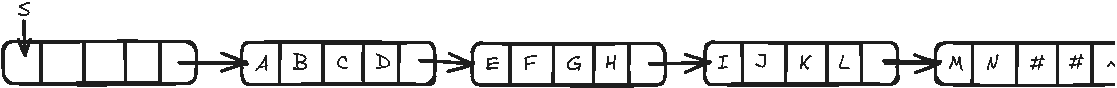
\includegraphics[width=0.8\textwidth]{./figure/pdf/cropped/linkStr_fourNodes.pdf}
  \caption{结点大小为4的链串}
  \label{fig:linkStr_fourNodes}

\end{figure}

\begin{figure}[!htbp]
  \centering
  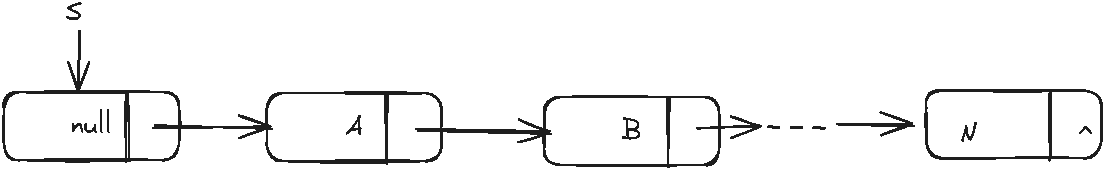
\includegraphics[width=0.6\textwidth]{./figure/pdf/cropped/linkStr_oneNode.pdf}
  \caption{结点大小为1的链串}
  \label{fig:linkStr_oneNode}

\end{figure}

当绪点大小大于 1(例如结点大小为4)时,链串的尾结点的各个数据域不一定总能全被
字符占满,此时应在这些未占用的数据域里补上不属于字符集的特殊符号(例如' \# '字符),
以示区别(参见图\ref{fig:linkStr_fourNodes} 中的尾结点) 。

在链串中 ,结点大小越大,存储密度越大,但一些基本操作(如插入、删除、替换等)有所
不便,且可能引起大量字符移动,因此它适合于串很少修改的情况; 结点大小越小(如结点
大小为 1 时) ,相关操作的实现越方便,但存储密度下降。为简便起见,这里规定链串结点大
小均为1。

链串的结构如代码\ref{lst:linkStringStruct}所示。

\begin{lstlisting}[language=C++, caption={链串结构体定义}, label={lst:linkStringStruct}]
  struct LinkNode {
    char data;//存放字符
    LinkNode* next;//指向下一个结点
  };

  struct LinkString {
    LinkNode* head;//头结点
    int length;//串的长度
  };
\end{lstlisting}

\section{串的操作}

串的操作包括创建、销毁、清空、获取长度、获取字符、连接、比较、插入、删除、替换、复制、判断相等、求子串、输出等。

\textbf{创建操作}:

创建一个空串,需要为串分配内存空间,并初始化串的长度。

代码如代码\ref{lst:createLinkString}所示。

\begin{lstlisting}[language=C++, caption={创建一个空串示例代码}, label={lst:createLinkString}]
  LinkString* createLinkString() {
    LinkString* s = (LinkString*)malloc(sizeof(LinkString));
    s->head = NULL;
    s->length = 0;
    return s;
  }

\end{lstlisting}

该算法的总时间复杂度为 $O(1)$,空间复杂度为 $O(1)$。


\textbf{销毁操作}:

销毁串,需要释放串的内存空间。

代码如代码\ref{lst:destroyLinkString}所示。

\begin{lstlisting}[language=C++, caption={销毁串示例代码}, label={lst:destroyLinkString}]
  void destroyLinkString(LinkString* s) {
    LinkNode* p = s->head;
    while (p != NULL) {
      LinkNode* q = p;
      p = p->next;
      free(q);
    }
    free(s);
  }

\end{lstlisting}

该算法的总时间复杂度为 $O(n)$,空间复杂度为 $O(1)$。


\textbf{清空操作}:

清空串,即将串的长度设置为0。

代码如代码\ref{lst:clearLinkString}所示。

\begin{lstlisting}[language=C++, caption={清空串示例代码}, label={lst:clearLinkString}]
  void clearLinkString(LinkString* s) {
    LinkNode* p = s->head;
    while (p != NULL) {
      LinkNode* q = p;
      p = p->next;
      free(q);
    }
    s->head = NULL;
    s->length = 0;
  }

\end{lstlisting}

该算法的总时间复杂度为 $O(n)$,空间复杂度为 $O(1)$。


\textbf{获取长度操作}:

获取串的长度。

代码如代码\ref{lst:lengthLinkString}所示。

\begin{lstlisting}[language=C++, caption={获取串的长度示例代码}, label={lst:lengthLinkString}]
  int lengthLinkString(LinkString* s) {
    return s->length;
  }

\end{lstlisting}

该算法的总时间复杂度为 $O(1)$,空间复杂度为 $O(1)$。


\textbf{获取字符操作}:

获取串中指定位置的字符。

代码如代码\ref{lst:getLinkString}所示。

\begin{lstlisting}[language=C++, caption={获取串中指定位置的字符示例代码}, label={lst:getLinkString}]
  char getLinkString(LinkString* s, int i) {
    if (i < 0 || i >= s->length) {
      printf(``位置不合法\n``);
      return -1;
    }
    LinkNode* p = s->head;
    for (int j = 0; j < i; j++) {
      p = p->next;
    }
    return p->data;
  }

\end{lstlisting}

该算法的总时间复杂度为 $O(n)$,空间复杂度为 $O(1)$。


\textbf{连接操作}:

连接两个串,即将两个串连接成一个串。

代码如代码\ref{lst:concatLinkString}所示。

\begin{lstlisting}[language=C++, caption={连接两个串示例代码}, label={lst:concatLinkString}]
  LinkString* concatLinkString(LinkString* s1, LinkString* s2) {
    LinkString* s = createLinkString();//创建一个新串
    LinkNode* p = s1->head;//将s1中的字符复制到s中
    
    while (p != NULL) {//复制s1中的字符
      LinkNode* q = (LinkNode*)malloc(sizeof(LinkNode));//创建一个新结点
      q->data = p->data;//复制字符
      q->next = NULL;
      if (s->head == NULL) {//将新结点插入到s中
        s->head = q;
      } else {//将新结点插入到s的末尾
        LinkNode* r = s->head;
        while (r->next != NULL) {
          r = r->next;
        }
        r->next = q;
      }
      s->length++;
      p = p->next;
    }
    p = s2->head;//将s2中的字符复制到s中
    while (p != NULL) {//复制s2中的字符
      LinkNode* q = (LinkNode*)malloc(sizeof(LinkNode));//创建一个新结点
      q->data = p->data;
      q->next = NULL;
      if (s->head == NULL) {//将新结点插入到s中
        s->head = q;
      } else {//将新结点插入到s的末尾
        LinkNode* r = s->head;
        while (r->next != NULL) {
          r = r->next;
        }
        r->next = q;
      }
      s->length++;
      p = p->next;
    }
    return s;
  }



\end{lstlisting}


\textbf{比较操作}:

比较两个串的大小。

代码如代码\ref{lst:compareLinkString}所示。

\begin{lstlisting}[language=C++, caption={比较两个串的大小示例代码}, label={lst:compareLinkString}]
  int compareLinkString(LinkString* s1, LinkString* s2) {//s1>s2返回正数,s1=s2返回0,s1<s2返回负数
    LinkNode* p = s1->head;
    LinkNode* q = s2->head;
    while (p != NULL && q != NULL) {//比较两个串的公共部分
      if (p->data != q->data) {//如果两个串的字符不相等
        return p->data - q->data;
      }
      p = p->next;
      q = q->next;
    }
    return s1->length - s2->length;
  }

\end{lstlisting}

\textbf{插入操作}:

在指定位置插入子串。

代码如代码\ref{lst:insertLinkString}所示。

\begin{lstlisting}[language=C++, caption={在指定位置插入子串示例代码}, label={lst:insertLinkString}]
  void insertLinkString(LinkString* s, int i, LinkString* t) {
    if (i < 0 || i > s->length) {
      printf(``位置不合法\n``);
      return;
    }
    LinkNode* p = s->head;
    for (int j = 0; j < i - 1; j++) {//找到第i-1个结点
      p = p->next;
    }
    LinkNode* q = t->head;
    while (q != NULL) {//将t中的字符插入到s中
      LinkNode* r = (LinkNode*)malloc(sizeof(LinkNode));//创建一个新结点
      r->data = q->data;
      r->next = p->next;
      p->next = r;
      s->length++;
      p = r;
      q = q->next;
    }
  }

\end{lstlisting}

\textbf{删除操作}:

删除指定位置的子串。

代码如代码\ref{lst:deleteLinkString}所示。

\begin{lstlisting}[language=C++, caption={删除指定位置的子串示例代码}, label={lst:deleteLinkString}]
  void deleteLinkString(LinkString* s, int i, int len) {
    if (i < 0 || i >= s->length || len < 0 || i + len > s->length) {
      printf(``位置不合法\n``);
      return;
    }
    LinkNode* p = s->head;
    for (int j = 0; j < i - 1; j++) {//找到第i-1个结点
      p = p->next;
    }
    LinkNode* q = p->next;
    for (int j = 0; j < len; j++) {//删除子串
      LinkNode* r = q;
      q = q->next;
      free(r);
      s->length--;
    }
    p->next = q;
  }

\end{lstlisting}

\textbf{替换操作}:

替换指定位置的子串。

代码如代码\ref{lst:replaceLinkString}所示。

\begin{lstlisting}[language=C++, caption={替换指定位置的子串示例代码}, label={lst:replaceLinkString}]
  void replaceLinkString(LinkString* s, int i, int len, LinkString* t) {
    if (i < 0 || i >= s->length || len < 0 || i + len > s->length) {
      printf(``位置不合法\n``);
      return;
    }
    LinkNode* p = s->head;
    for (int j = 0; j < i - 1; j++) {//找到第i-1个结点
      p = p->next;
    }
    LinkNode* q = p->next;
    for (int j = 0; j < len; j++) {//删除子串
      LinkNode* r = q;
      q = q->next;
      free(r);
      s->length--;
    }
    p->next = q;
    LinkNode* r = t->head;
    while (r != NULL) {//插入子串
      LinkNode* s = (LinkNode*)malloc(sizeof(LinkNode));//创建一个新结点
      s->data = r->data;
      s->next = p->next;
      p->next = s;
      s->length++;
      p = s;
      r = r->next;
    }
  }

\end{lstlisting}

\textbf{复制操作}:

复制串。

代码如代码\ref{lst:copyLinkString}所示。

\begin{lstlisting}[language=C++, caption={复制串示例代码}, label={lst:copyLinkString}]
  LinkString* copyLinkString(LinkString* s) {
    LinkString* t = createLinkString();
    LinkNode* p = s->head;
    LinkNode* q = NULL;
    while (p != NULL) {
      LinkNode* r = (LinkNode*)malloc(sizeof(LinkNode));
      r->data = p->data;
      r->next = NULL;
      if (t->head == NULL) {
        t->head = r;
      } else {
        q->next = r;
      }
      t->length++;
      q = r;
      p = p->next;
    }
    return t;
  }

\end{lstlisting}

\textbf{判断相等操作}:

判断两个串是否相等。

代码如代码\ref{lst:equalLinkString}所示。

\begin{lstlisting}[language=C++, caption={判断两个串是否相等示例代码}, label={lst:equalLinkString}]
  bool equalLinkString(LinkString* s1, LinkString* s2) {
    LinkNode* p = s1->head;
    LinkNode* q = s2->head;
    while (p != NULL && q != NULL) {
      if (p->data != q->data) {
        return false;
      }
      p = p->next;
      q = q->next;
    }
    return p == NULL && q == NULL;
  }

\end{lstlisting}

\textbf{求子串操作}:

求串的子串。

代码如代码\ref{lst:subLinkString}所示。

\begin{lstlisting}[language=C++, caption={求串的子串示例代码}, label={lst:subLinkString}]
  LinkString* subLinkString(LinkString* s, int i, int len) {
    if (i < 0 || i >= s->length || len < 0 || i + len > s->length) {
      printf(``位置不合法\n``);
      return NULL;
    }
    LinkString* t = createLinkString();
    LinkNode* p = s->head;
    for (int j = 0; j < i; j++) {
      p = p->next;
    }
    LinkNode* q = NULL;
    while (len > 0) {
      LinkNode* r = (LinkNode*)malloc(sizeof(LinkNode));
      r->data = p->data;
      r->next = NULL;
      if (t->head == NULL) {
        t->head = r;
      } else {
        q->next = r;
      }
      t->length++;
      q = r;
      p = p->next;
      len--;
    }
    return t;
  }

\end{lstlisting}

\textbf{输出操作}:

输出串。

代码如代码\ref{lst:printLinkString}所示。

\begin{lstlisting}[language=C++, caption={输出串示例代码}, label={lst:printLinkString}]
  void printLinkString(LinkString* s) {
    LinkNode* p = s->head;
    while (p != NULL) {
      printf(``%c``, p->data);
      p = p->next;
    }
    printf(``\n``);
  }

\end{lstlisting}


\section{串模式匹配}

设有两个串* 和+,,串上的定位就是要在串s 中找到一个与上相等的子串。通常把 * 称
为目标串(target string) ,把 上 称为模式串(pattern string),因此串定位查找也称为模式匹配
Cpattern matching) 。模式匹配成功是指在目标串 s 中找到了一个模式串 上; 不成功则指目
标串 * 中不存在模式串+。

模式匹配是一个比较复杂的串操作 ,许多人对此提出了很多效率各不相同的算法。在
此介绍两种算法 ,并设串均采用顺序存储结构 。

\subsection{BF算法}

BF(Brute Force)算法是一种简单直观的模式匹配算法,也称为朴素模式匹配算法。
BF算法的基本思想是从目标串的第一个字符开始,依次与模式串的每一个字符进行比较,如果相等,
则继续比较下一个字符,如果不相等,则从目标串的下一个字符开始,重新与模式串的第一个字符比较,
直到找到与模式串相等的子串或目标串的所有字符都比较完为止。

例如 ,设目标串为``ababcabcacbab``,模式串为``abcac``,BF算法的匹配过程如下:

\begin{itemize}
  \item 从目标串的第一个字符``a``开始,与模式串的第一个字符``a``比较,相等,继续比较下一个字符;
  \item 与模式串的第二个字符``b``比较,不相等,从目标串的第二个字符``b``开始,重新与模式串的第一个字符比较;
  \item 与模式串的第一个字符``a``比较,不相等,从目标串的第三个字符``a``开始,重新与模式串的第一个字符比较;
  \item 与模式串的第一个字符``a``比较,相等,继续比较下一个字符;
  \item 与模式串的第二个字符``b``比较,相等,继续比较下一个字符;
  \item 与模式串的第三个字符``c``比较,相等,继续比较下一个字符;
  \item 与模式串的第四个字符``a``比较,相等,继续比较下一个字符;
  \item 与模式串的第五个字符``c``比较,相等,匹配成功。
\end{itemize}

BF算法的代码如代码\ref{lst:BF}所示。

\begin{lstlisting}[language=C++, caption={BF算法示例代码}, label={lst:BF}]
  int BF(char* s, char* t) {
    int i = 0, j = 0;
    while (s[i] != '\0' && t[j] != '\0') {
      if (s[i] == t[j]) {
        i++;
        j++;
      } else {
        i = i - j + 1;
        j = 0;
      }
    }
    if (t[j] == '\0') {
      return i - j;
    } else {
      return -1;
    }
  }

\end{lstlisting}

BF算法的时间复杂度为$O(m*n)$,空间复杂度为$O(1)$。

这个算法简单且易于理解,但效率不高,主要原因是主串指针 $i$ 在若干个字符比较相等后,若有一个字符比较不相等,
就需回溯(即 $i = i - j + 1$)。该算法在最好情况下的时间复杂度为 $O(m)$,
即主串的前 $m$ 个字符正好等于模式串的 $m$ 个字符。在最坏情况下的时间复杂度为 $O(n \times m)$。
可以证明其平均时间复杂度也是 $O(n \times m)$,也就是说,该算法的平均时间性能接近最坏的情况。
\subsection{KMP算法}

KMP 算法是 D. E. Knuth、J. H. Morris 和 V. R. Pratt 共同提出的,称之为 Knuth-
Morris-Pratt 算法 ,简称 KMP 算法。该算法与 Brute-Force 算法相比有较大的改进,主要是
消除了主串指针的回溯,从而使算法效率有了某种程度的提高。

KMP算法的核心,是一个被称为部分匹配表(Partial Match Table)的数组。
这里我们抛开所有的枝枝蔓蔓,先来解释一下这个数据到底是什么。对于字符串“abababca”,它的PMT如表\ref{table:PMT}所示。


\begin{table}[htbp]
  \centering
  \caption{PMT表}
  \begin{tabular}{|c|c|c|c|c|c|c|c|c|}
    \hline
    字符串 & a & b & a & b & a & b & c & a \\
    \hline
    index: & 0 & 1 & 2 & 3 & 4 & 5 & 6 & 7 \\
    \hline
    PMT值 & 0 & 0 & 1 & 2 & 3 & 4 & 0 & 1 \\
    \hline
  \end{tabular}
  \label{table:PMT}
\end{table}

就像例子中所示,如果待匹配的模式字符串有8个字符,那么PMT就有8个值。

在这里要先解释一下字符串的前缀和后缀。所谓前缀,顾名思义,就是除了最后一个字符以外,一个字符串的全部头部组合;
后缀则是除了第一个字符以外,一个字符串的全部尾部组合。比如字符串“ABCD”的前缀包括“A”、“AB”和“ABC”,后缀包括“BCD”、“CD”和“D”。

例如,对于字符串“abababca”,它的前缀和后缀的匹配情况如下:

\begin{itemize}
  \item “a”:前缀为空集,后缀为空集,匹配长度为0;
  \item “ab”:前缀为{“a”},后缀为{“b”},匹配长度为0;
  \item “aba”:前缀为{“a”,“ab”},后缀为{“ba”,“a”},匹配长度为1;
  \item “abab”:前缀为{“a”,“ab”,“aba”},后缀为{“bab”,“ab”,“b”},匹配长度为2;
  \item “ababa”:前缀为{“a”,“ab”,“aba”,“abab”},后缀为{“baba”,“aba”,“ba”,“a”},匹配长度为3;
  \item “ababab”:前缀为{“a”,“ab”,“aba”,“abab”,“ababa”},后缀为{“babab”,“abab”,“bab”,“ab”,“b”},匹配长度为4;
  \item “abababc”:前缀为{“a”,“ab”,“aba”,“abab”,“ababa”,“ababab”},后缀为{“bababc”,“ababc”,“babc”,“abc”,“bc”,
  
  “c”},匹配长度为0;
  \item “abababca”:前缀为{“a”,“ab”,“aba”,“abab”,“ababa”,“ababab”,“abababc”},后缀为{“babca”,“abca”,“bca”,“ca”,“a”},匹配长度为1。
\end{itemize}

有了这个定义,就可以说明PMT的含义了。PMT的值是字符串的前缀集合与后缀集合的交集中最长元素的长度。


在清楚这个表所表达的意思之后,我们再来看看如何使用这个表来加速字符串的查找,以及这样使用的道理是什么。

如图\ref{fig:KMP}所示,当模式串与主串匹配失败时,根据PMT表,模式串向右移动的位数为失配字符的位置减去对应的PMT值。

\begin{figure}[!htbp]
  \centering
  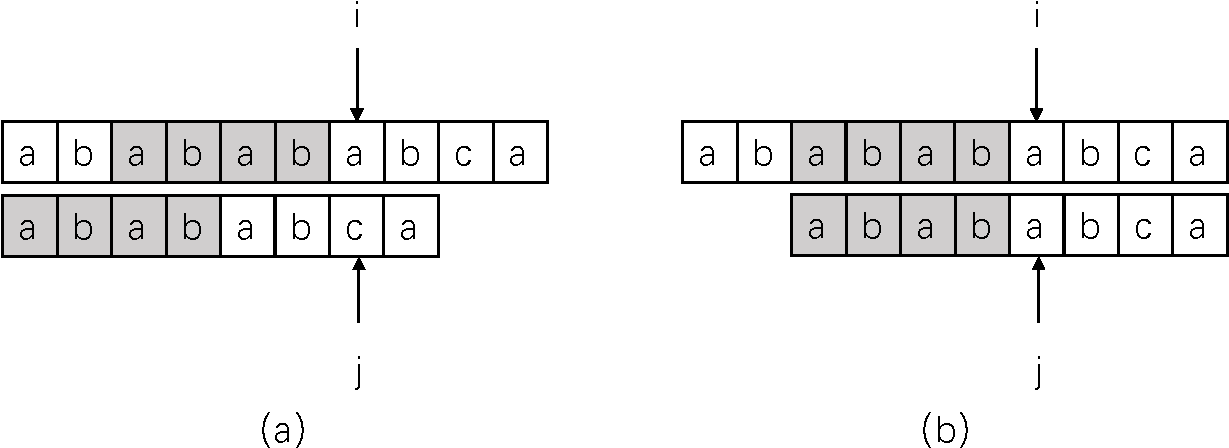
\includegraphics[width=0.5\textwidth]{./figure/pdf/cropped/KMP.pdf}
  \caption{KMP算法示意图}
  \label{fig:KMP}

\end{figure}

在主字符串 ``ababababca`` 中查找模式字符串 ``abababca`` 时,如果在位置 j 处字符不匹配,根据模式字符串的 PMT(部分匹配表)性质,可以跳过一些字符的比较。

假设主字符串的 i 指针在位置 i 处失配,这意味着主字符串从位置 i−j 到 i 的这一段,与模式字符串从位置 0 到 j 的这一段是完全相同的。而 PMT[j−1] 表示模式字符串从位置 0 到 j−1 的最长前缀和后缀的匹配长度。

因此,我们可以断定主字符串中 i 指针之前的 PMT[j−1] 位,与模式字符串的第 0 位到第 PMT[j−1] 位是相同的。这样一来,这些字符的比较就可以跳过。

具体做法是:

1. 保持主字符串的 i 指针不动。

2. 将模式字符串的 j 指针移动到 PMT[j−1] 位置。

例如,在位置 i 处失配时,主字符串和模式字符串的前 6 位是相同的。而模式字符串的前 6 位中,其前 4 位的前缀和后 4 位的后缀是相同的。
因此,我们可以推断主字符串中 i 指针之前的 4 位,与模式字符串开头的 4 位是相同的(即灰色部分)。这部分无需再次比较。并且我们知道根据
PMT表就已经是最长公共前后缀了,所以我们可以放心的将模式串的指针移动到 PMT[j−1] 位置。

有了上面的思路,我们就可以使用PMT加速字符串的查找了。
我们看到如果是在 j 位 失配,那么影响 j 指针回溯的位置的其实是第 j −1 位的 PMT 值,所以为了编程的方便, 
我们不直接使用PMT数组,而是将PMT数组向后偏移一位。我们把新得到的这个数组称为next数组。
下面给出根据next数组进行字符串匹配加速的字符串匹配程序。其中要注意的一个技巧是,
在把PMT进行向右偏移时,第0位的值,我们将其设成了-1,这只是为了编程的方便,并没有其他的意义。
在本节的例子中,next数组如表\ref{table:next}所示。


\begin{table}[htbp]
  \centering
  \caption{PMT与next表对比}
  \begin{tabular}{|c|c|c|c|c|c|c|c|c|}
    \hline
    字符串 & a & b & a & b & a & b & c & a \\
    \hline
    index: & 0 & 1 & 2 & 3 & 4 & 5 & 6 & 7 \\
    \hline
    PMT值 & 0 & 0 & 1 & 2 & 3 & 4 & 0 & 1 \\
    \hline
    next值 & -1 & 0 & 0 & 1 & 2 & 3 & 4 & 0 \\
    \hline
  \end{tabular}
  \label{table:next-PMT}
\end{table}

KMP算法的代码如代码\ref{lst:KMP}所示。

\begin{lstlisting}[language=C++, caption={KMP算法示例代码}, label={lst:KMP}]
  void getNext(char* t, int* next) {
    int j = 0, k = -1;
    next[0] = -1;
    while (t[j] != '\0') {
      if (k == -1 || t[j] == t[k]) {
        j++;
        k++;
        next[j] = k;
      } else {
        k = next[k];
      }
    }
  }

  int KMP(char* s, char* t) {
    int i = 0, j = 0;
    int next[100];
    getNext(t, next);
    while (s[i] != '\0' && t[j] != '\0') {
      if (j == -1 || s[i] == t[j]) {
        i++;
        j++;
      } else {
        j = next[j];
      }
    }
    if (t[j] == '\0') {
      return i - j;
    } else {
      return -1;
    }
  }

\end{lstlisting}


KMP算法的时间复杂度为$O(m+n)$,空间复杂度为$O(m)$。


在上述代码中,我们使用到了一个next数组,在之前的学习中我们知道所谓next数组就是PMT表的变形,现在我们一起来看看如何求解next数组。

\subsection{next数组的求解}

前缀表存储每一个前缀的最长公共前后缀的长度,next数组存储的是模式串向右移动到next值的位置,这个值与前缀的最长公共前后缀的长度有关,所以next数组是可以由前缀表生成的。

用前缀表生成一个next数组很容易,将前缀表每一位都向后移动1位(最后一位舍去)并在第一位补一个-1就得到了next数组。

next与PMT对比表如表\ref{table:next-PMT}所示。

\begin{table}[htbp]
  \centering
  \caption{next表}
  \begin{tabular}{|c|c|c|c|c|c|c|c|c|}
    \hline
    字符串 & a & b & a & b & a & b & c & a \\
    \hline
    index: & 0 & 1 & 2 & 3 & 4 & 5 & 6 & 7 \\
    \hline
    next值 & -1 & 0 & 0 & 1 & 2 & 3 & 4 & 0 \\
    \hline
  \end{tabular}
  \label{table:next}
\end{table}

\textbf{为什么有些 next 数组是 $0, 1$ 开头,而有些是 $-1, 0$ 开头}

$-1, 0$ 开头与 $0, 1$ 开头的 next 数组本质是一样的。实际上,以 $0, 1$ 开头的 next 数组就是以 $-1, 0$ 开头的 next 数组每一项加 1 得到的。

出现这种情况的原因在于模式串起始的索引值:
\begin{itemize}
  \item 在程序中,一个数组的索引的起始值为 $0$;
  \item 然而在考试和书中给的模式串起始值通常从 $1$ 开始。
\end{itemize}

因此:
\begin{itemize}
  \item 在考试中遇到的 next 数组通常是以 $0, 1$ 开头;
  \item 而一些程序或教程中的 next 数组是以 $-1, 0$ 开头。
\end{itemize}

\textbf{注}:在考试中通常会给出模式串的索引,或者会给出 next 值的前两项。在答题时,应按照题目中的要求书写 next 数组。


求解next数组的代码如代码\ref{lst:next}所示。

\begin{lstlisting}[language=C++, caption={求解next数组示例代码}, label={lst:next}]
  // 求解next数组
void getNext(const std::string &pattern, std::vector<int> &next) {
  int m = pattern.size();
  next.resize(m);
  next[0] = -1; // 初始化第一个位置为 -1
  int j = 0, k = -1;

  while (j < m - 1) {
    if (k == -1 || pattern[j] == pattern[k]) {
      ++j;
      ++k;
      next[j] = k; // 更新 next 数组
    } else {
      k = next[k]; // 回溯
    }
  }
}

\end{lstlisting}
\chapter{数组和广义表}

\section{数组}

\subsection{数组的基本概念}

从逻辑结构上看,数组是具有相同数据类型的有限个数据元素的有序序列。

从存储结构上看,数组是一种顺序存储结构,它的元素在内存中是连续存储的。

几乎所有的计算机高级语言都实现了数组这种数据结构,数组是一种非常重要的数据结构,它在计算机程序设计中有着广泛的应用。
这里以C语言为例,介绍数组的基本性质:

\begin{itemize}
  \item 数组的长度:数组的长度是数组中元素的个数,数组的长度是固定的,一旦定义就不能改变。
  \item 数组的下标:数组的下标是从0开始的整数,数组的第一个元素的下标为0,第二个元素的下标为1,依次类推。
  \item 数组的元素:数组的元素是具有相同数据类型的数据元素,数组的元素可以是基本数据类型,也可以是结构体、类等复合数据类型。
  \item 数组的随机访问:数组的元素可以通过下标随机访问,数组的随机访问时间复杂度为O(1)。
\end{itemize}
\subsection{数组的存储结构}

在设计数组的存储结构时,通常将数组的所有元素存储到一块连续的内存空间中,这样可以通过数组的下标随机访问数组的元素。
\subsubsection{一维数组的存储结构}

对于一维数组 $(a_1, a_2, \dots, a_i, \dots, a_n)$,按元素顺序存储到一块地址连续的内存单元中。  
假设第一个元素 $a_1$ 的存储地址用 $\text{LOC}(a_1)$ 表示,每个元素占用 $R$ 个存储单元,则任一数组元素 $a_i$ 的存储地址 $\text{LOC}(a_i)$ 即可由以下公式求出:

\begin{equation}
    \text{LOC}(a_i) = \text{LOC}(a_1) + (i - 1) \times R \quad (1 \leq i \leq n)
\end{equation}

该式说明一维数组中任一元素的存储地址可直接计算得到,即一维数组中的任一元素可直接存取,正因为如此,一维数组具有随机存储特性。
\subsubsection{二维数组的存储结构}

对于一个 $m$ 行 $n$ 列的二维数组 $A_{m \times n}$:

\[
\begin{bmatrix}
a_{0,0} & a_{0,1} & \dots & a_{0,n-1} \\
a_{1,0} & a_{1,1} & \dots & a_{1,n-1} \\
\vdots & \vdots & \ddots & \vdots \\
a_{m-1,0} & a_{m-1,1} & \dots & a_{m-1,n-1}
\end{bmatrix}
\]

将 $A_{m \times n}$ 简记为 $A$,$A$ 是这样的一维数组:
\[
A = (a_{0,0}, a_{0,1}, \dots, a_{0,n-1}, a_{1,0}, a_{1,1}, \dots, a_{m-1,n-1})
\]
其中,$a_{i,j}$ 表示二维数组中第 $i$ 行第 $j$ 列的元素,$0 \leq i \leq m -1 , 0 \leq j \leq n-1$。

对于二维数组来说,其存储方式主要有两种,即按行优先存放(或者以行序为主序存放)和按列优先存放(或者以列序为主序存放)。

\textbf{二维数组按行优先存放}

二维数组按行优先存放的示意图如图\ref{fig:row_major_array}所示,即先存储第 1 行,紧接着存储第 2 行……依此类推,最后存储第 $m$ 行。

\[
\begin{bmatrix}
a_{0,0} & a_{0,1} & \dots & a_{0,n-1} \\
a_{1,0} & a_{1,1} & \dots & a_{1,n-1} \\
\vdots & \vdots & \ddots & \vdots \\
a_{m-1,0} & a_{m-1,1} & \dots & a_{m-1,n-1}
\end{bmatrix}
\]

\begin{figure}[!htbp]
  \centering
  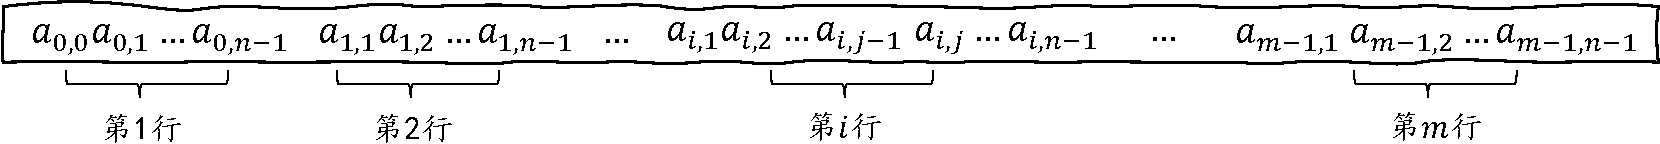
\includegraphics[width=1\textwidth]{./figure/pdf/cropped/rowFirst.pdf}
  \caption{二维数组按行优先存储的一维数组表示(下标从0开始)}
  \label{fig:row_major_array}
\end{figure}

假设第一个元素 $a_{0,0}$ 的存储地址用 $\text{LOC}(a_{0,0})$ 表示,每个元素占用 $R$ 个存储单元,则该二维数组中的任一元素 $a_{i,j}$ 的存储地址可由下式确定:

\begin{equation}
\text{LOC}(a_{i,j}) = \text{LOC}(a_{0,0}) + [i \times n + j] \times R
\end{equation}

上式推导的思路是,在内存中元素 $a_{i,j}$ 前面有 $i$ 行,每行 $n$ 个元素,即已存放了 $i \times n$ 个元素,占用了 $i \times n \times R$ 个内存单元;在第 $i$ 行中,元素 $a_{i,j}$ 前面有 $j$ 个元素,即已存放了 $j$ 个元素,占用了 $j \times R$ 个内存单元。因此,元素 $a_{i,j}$ 的存储地址为上述公式所示。

\textbf{二维数组按列优先存放}

二维数组按列优先存放的示意图如图\ref{fig:column_major_array}所示,即先存储第 0 列,紧接着存储第 1 列……依此类推,最后存储第 $n-1$ 列。

\[
\begin{bmatrix}
a_{0,0} & a_{0,1} & \dots & a_{0,n-1} \\
a_{1,0} & a_{1,1} & \dots & a_{1,n-1} \\
\vdots & \vdots & \ddots & \vdots \\
a_{m-1,0} & a_{m-1,1} & \dots & a_{m-1,n-1}
\end{bmatrix}
\]

\begin{figure}[!htbp]
  \centering
  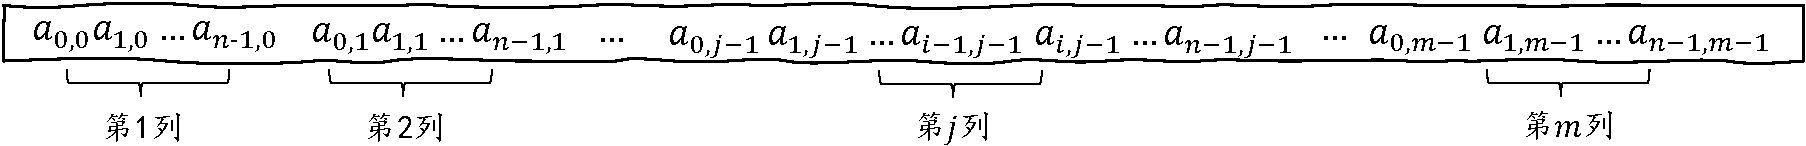
\includegraphics[width=1\textwidth]{./figure/pdf/cropped/columnFirst.pdf}
  \caption{二维数组按列优先存储的一维数组表示(下标从0开始)}
  \label{fig:column_major_array}
\end{figure}

假设第一个元素 $a_{0,0}$ 的存储地址用 $\text{LOC}(a_{0,0})$ 表示,每个元素占用 $R$ 个存储单元,则该二维数组中的任一元素 $a_{i,j}$ 的存储地址可由下式确定:

\begin{equation}
\text{LOC}(a_{i,j}) = \text{LOC}(a_{0,0}) + [j \times m + i] \times R
\end{equation}

上式推导的思路是,在内存中元素 $a_{i,j}$ 前面有 $j$ 列,每列 $m$ 个元素,即已存放了 $j \times m$ 个元素,占用了 $j \times m \times R$ 个内存单元;在第 $j$ 列中,元素 $a_{i,j}$ 前面有 $i$ 个元素,即已存放了 $i$ 个元素,占用了 $i \times R$ 个内存单元。因此,元素 $a_{i,j}$ 的存储地址为上述公式所示。

特殊矩阵是指非零元素或零元素的分布有一定规律的矩阵,为了节省存储空间 ,特别是在
高阶矩阵的情况下 ,可以利用特殊矩阵的规律对它们进行压缩存储,以提高存储空间效率。
特殊和矩阵的主要形式有对称和矩阵、对角和抑阵等。它们都是方阵 ,即行数和列数相同。

\textbf{对称矩阵的压缩存储}

对称矩阵是指矩阵的元素以主对角线为对称轴对应相等的矩阵,即 $a_{i,j} = a_{j,i}$,对称矩阵的主对角线上的元素都是对称轴上的元素。

对称矩阵的压缩存储方法是只存储矩阵的上三角元素或下三角元素,这样可以节省一半的存储空间。


若一个阶为 $n$ 的方阵 $A$ 中的元素满足 $a_{i,j} = a_{j,i} \ (0 \leq i, j \leq n-1)$,则称其为 $n$ 阶对称矩阵(symmetric matrix)。

一般情况下,一个 $n$ 阶方阵的所有元素可以分为 3 个部分,即主对角部分(含 $n$ 个元素)、上三角部分和下三角部分,如图\ref{fig:common_matrix}所示。
已知一个元素的下标,就可以确定它属于哪个部分。

\begin{figure}[!htbp]
  \centering
  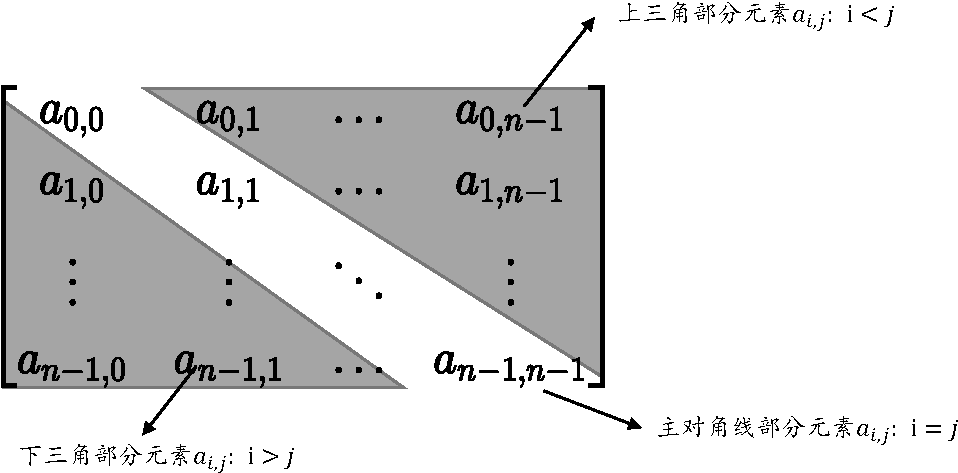
\includegraphics[width=0.5\textwidth]{./figure/pdf/cropped/commonMatrix.pdf}
  \caption{一般矩阵的三个部分}
  \label{fig:common_matrix}
\end{figure}

对称矩阵中的元素是按对角线对称的,即上三角部分和下三角部分中的对应元素相等,因此在存储时可以只存储主对角线加上三角部分的元素,
或者主对角线加下三角部分的元素,让对称的两个元素共享一个存储空间。

不失一般性,对称矩阵采用以行序为主序存储主对角线加下三角部分的元素。如图\ref{fig:downMatrix}所示,假设以一维数组

\begin{figure}
  \centering
  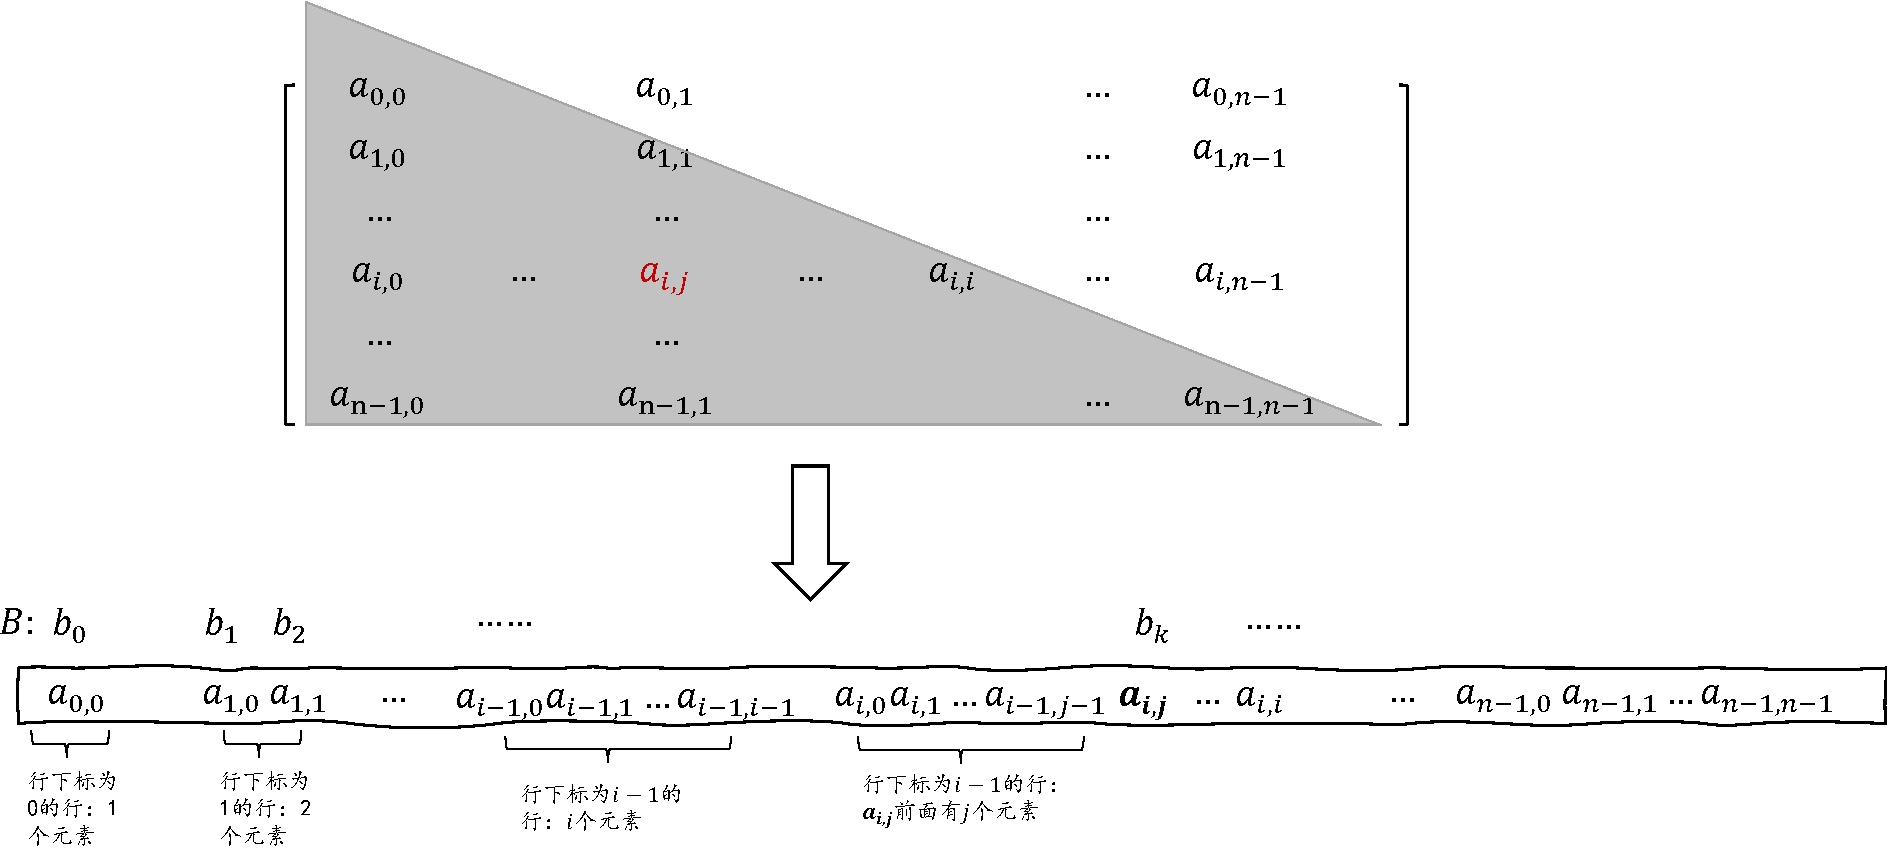
\includegraphics[width=1\textwidth]{./figure/pdf/cropped/downMatrix.pdf}
  \caption{对称矩阵的压缩存储}
  \label{fig:downMatrix}
\end{figure}
\[
B[0 \dots \frac{n(n+1)}{2} - 1]
\]

作为 $n$ 阶对称矩阵 $A$ 的存储结构,$A$ 中的元素 $a_{i,j}$ 存储在 $B$ 中的元素 $B[k]$ 中,那么 $k$ 与 $i,j$ 的关系分为以下
两种情况:

(1) 若 $a_{i,j}$ 是 $A$ 中主对角线或者下三角部分的元素,有 $i \geq j$。在以行序为主序的存储方式下,不计行下标为 $i$ 的行,
元素 $a_{i,j}$ 的前面共存储了 $i$ 行(行下标为 $0$ 到 $i-1$,行下标为 $0$ 的行有一个元素,行下标为 $1$ 的行有两个元素,……,
行下标为 $i-1$ 的行有 $i$ 个元素),这 $i$ 行有 $1 + 2 + \dots + i = \frac{i(i+1)}{2}$ 个元素;在行下标为 $i$ 的行中,
元素 $a_{i,j}$ 的前面也存储了 $j$ 个元素。所以元素 $a_{i,j}$ 的前面共存储了 $\frac{i(i+1)}{2} + j$ 个元素,而一维数组的下标
是从 $0$ 开始的,所以有:
\[
k = \frac{i(i+1)}{2} + j
\]

(2) 若 $a_{i,j}$ 是 $A$ 中上三角部分的元素,有 $i < j$。其值等于 $a_{j,i}$,而元素 $a_{j,i}$ 属于情况 (1),它存放在 $B$ 中
下标为 $k = \frac{j(j+1)}{2} + i$ 的位置,所以此时有:
\[
k = \frac{j(j+1)}{2} + i
\]

将两种情况合起来,得到 $k$ 与 $i,j$ 的关系如下:
\[
k =
\begin{cases} 
\frac{i(i+1)}{2} + j, & \text{当 } i \geq j \\ 
\frac{j(j+1)}{2} + i, & \text{当 } i < j 
\end{cases}
\]

显然,一维数组 $B$ 中存放的元素个数为 $1 + 2 + \dots + n = \frac{n(n+1)}{2}$。如果将 $A$ 直接采用一个 $n \times n$ 的二维数组存储,所需要的存储空间为 $n^2$ 个元素,所以这种压缩存储方法几乎节省了一半的存储空间。另外,由于一维数组 $B$ 具有随机存取特性,所以采用这种压缩存储方法后,对称矩阵 $A$ 仍然具有随机存取特性。

归纳起来,在计算 $A$ 中元素 $a_{i,j}$ 在 $B$ 中存储位置 $k$ 时,首先求出元素 $a_{i,j}$ 前面共存放多少个元素(设为 $m$ 个);再看 $B$ 中存放元素的下标是从 $0$ 开始还是从 $1$ 开始(设 $B$ 的初始下标为 $s$),则有:
\[
k = m + s
\]
\textbf{上、下三角矩阵的压缩存储}

上、下三角矩阵是指矩阵的主对角线以下(或以上)的元素都是零的矩阵。上三角矩阵是指主对角线以下的元素都是零的矩阵,下三角矩阵是指主对角线以上的元素都是零的矩阵。

上、下三角矩阵的压缩存储方法是只存储矩阵的上三角元素或下三角元素,这样可以节省一半的存储空间。

我们以上三角矩阵为例,对于上三角矩阵,其压缩存储方法是采用以行序为主序存储其主对角线加上三角部分的元素,
另外用一个元素存储常数 $c$,并将压缩结果存放在一维数组 $B$ 中,如图\ref{fig:upperMatrix}所示。

\begin{figure}[!htbp]
  \centering
  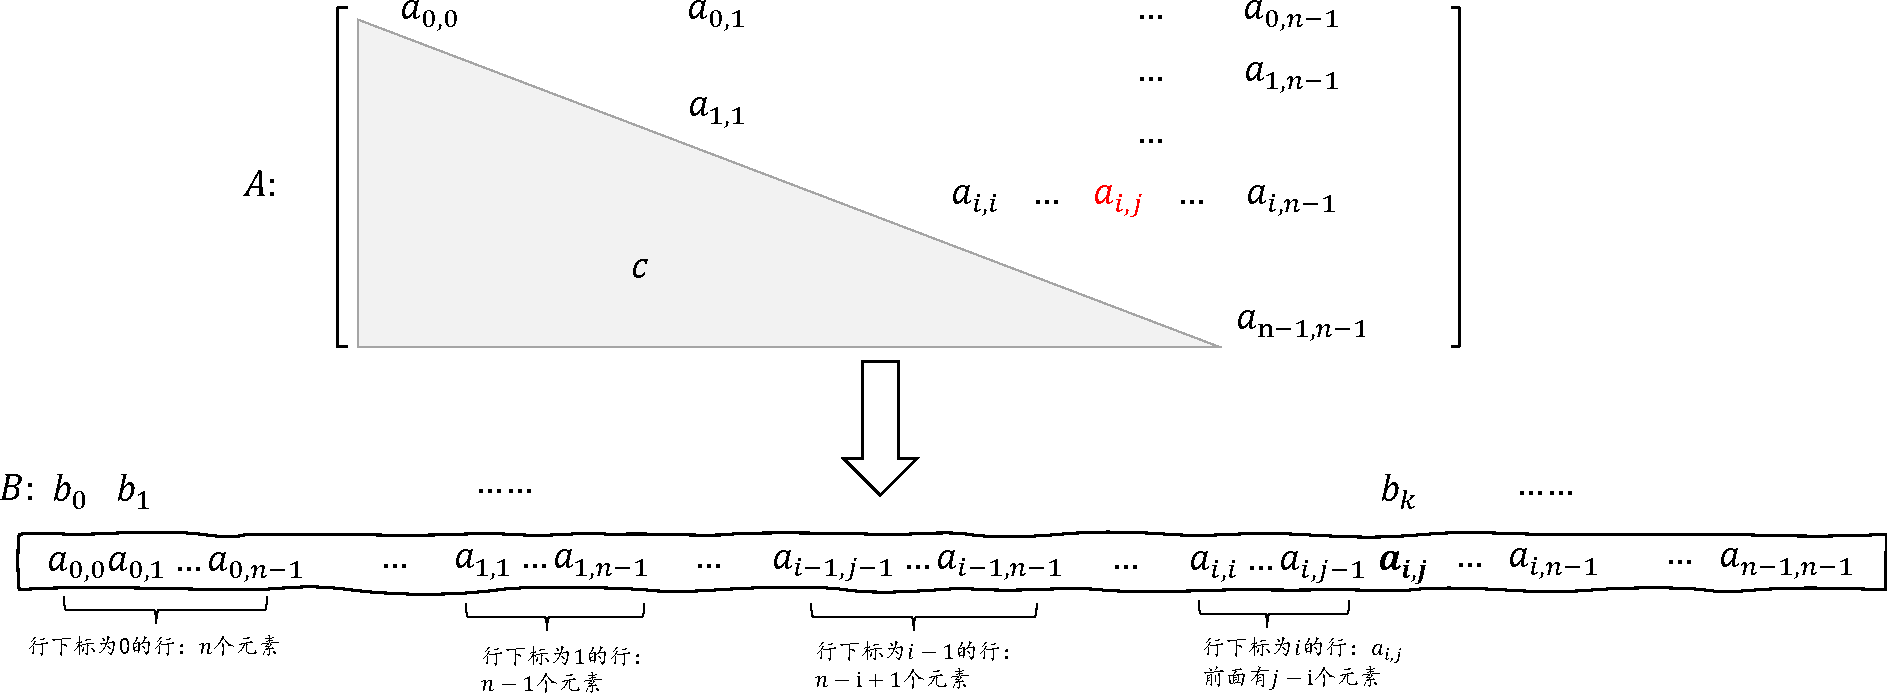
\includegraphics[width=1\textwidth]{./figure/pdf/cropped/upperMatrix.pdf}
  \caption{上三角矩阵的压缩存储}
  \label{fig:upperMatrix}
\end{figure}
显然,$B$ 中元素的个数为 $\frac{n(n+1)}{2} + 1$,即用 $B[0 \dots \frac{n(n+1)}{2}]$ 存放矩阵 $A$ 中的元素。

同样,$A$ 中元素 $a_{i,j}$ 存储在 $B$ 的元素 $B[k]$ 中,那么 $k$ 与 $i,j$ 的关系分为以下两种情况:

(1) 若 $a_{i,j}$ 是 $A$ 中主对角线或者上三角部分的元素,有 $i \leq j$。在以行序为主序的存储方式下,不计行下标为 $i$ 的行,元素 $a_{i,j}$ 的前面共存储了 $i$ 行(行下标为 $0 \sim i-1$,行下标为 $0$ 的行有 $n$ 个元素,行下标为 $1$ 的行有 $n-1$ 个元素,……,行下标为 $i-1$ 的行有 $n-i+1$ 个元素),这 $i$ 行有:
\[
n + (n-1) + \dots + (n-i+1) = \frac{i(2n-i+1)}{2}
\]
个元素;在行下标为 $i$ 的行中,元素 $a_{i,j}$ 的前面也存储了 $j-i$ 个元素。所以元素 $a_{i,j}$ 的前面共存储了:
\[
\frac{i(2n-i+1)}{2} + (j-i)
\]
个元素,而一维数组的下标是从 $0$ 开始的,所以有:
\[
k = \frac{i(2n-i+1)}{2} + (j-i)
\]

(2) 若 $a_{i,j}$ 是 $A$ 中下三角部分的元素,有 $i > j$。其值为常数 $c$,用 $B$ 中最后一个位置(即下标为 $\frac{n(n+1)}{2}$ 的元素)存放常数 $c$。

将两种情况合起来,得到 $k$ 与 $i,j$ 的关系如下:
\[
k =
\begin{cases} 
\frac{i(2n-i+1)}{2} + (j-i), & \text{当 } i \leq j \\ 
\frac{n(n+1)}{2}, & \text{当 } i > j
\end{cases}
\]

对于下三角矩阵 $A$,其常见的压缩存储方法是采用以行序为主序存储其主对角线加下三角部分的元素,另外用一个元素存储常数 $c$,
并将压缩结果存放在一维数组 $B$ 中。采用类似于对称矩阵的推导过程,得到 $k$ 与 $i,j$ 的关系如下:
\[
k =
\begin{cases} 
\frac{i(2n-i+1)}{2} + (j-i), & \text{当 } i \leq j \\ 
\frac{n(n+1)}{2}, & \text{当 } i > j
\end{cases}
\]
\section{稀疏矩阵}



\subsection{稀疏矩阵的定义}

稀疏矩阵是指矩阵中绝大多数元素为零的矩阵。在实际应用中,许多矩阵都是稀疏矩阵,例如,图像处理中的二值图像、灰度图像等。

例如 $m \times n$ 的矩阵 $A$ 如表\ref{table:sparse_matrix}所示,其中 $m = 6$,$n = 7$

\begin{table}[htbp]
  \centering
  \caption{稀疏矩阵示例}
  \begin{tabular}{||ccccccc||c}
    
    1 & 0 & 3 & 0 & 0 & 0 & 0 \\
    0 & 2 & 0 & 0 & 0 & 0 & 0 \\
    4 & 0 & 5 & 0 & 0 & 0 & 0 \\
    0 & 0 & 0 & 0 & 9 & 0 & 0 \\
    0 & 0 & 0 & 0 & 0 & 0 & 0 \\
    0 & 0 & 0 & 0 & 0 & 0 & 4 \\
    
  \end{tabular}
  \label{table:sparse_matrix}
\end{table}

在表\ref{table:sparse_matrix}中,矩阵 $A$ 中有 $t = 7$ 个非零元素,占矩阵 $A$ 的总元素个数的比例为 $\frac{t}{m \times n} = \frac{7}{42} \approx 0.1667$,因此矩阵 $A$ 是一个稀疏矩阵。

\subsection{稀疏矩阵的三元组表示}

稀疏矩阵的三元组表示是指用三个一维数组来表示稀疏矩阵,这三个数组分别存储非零元素的行号、列号和元素值。


\begin{table}[htbp]
  \centering
  \caption{稀疏矩阵的三元组表示}
  \begin{tabular}{|c|c|c|}
    \hline
    行号 & 列号 & 元素值 \\
    \hline
    0 & 0 & 1 \\
    0 & 2 & 3 \\
    1 & 1 & 2 \\
    2 & 0 & 4 \\
    2 & 2 & 5 \\
    3 & 4 & 9 \\
    5 & 6 & 4 \\
    \hline
  \end{tabular}
  \label{table:sparse_matrix_triplet}
\end{table}

表\ref{table:sparse_matrix_triplet}中的三元组表示了表\ref{table:sparse_matrix}中的稀疏矩阵,其中第一列存储了非零元素的行号,第二列存储了非零元素的列号,第三列存储了非零元素的值。

三元组顺序表的数据类型定义如下:

\begin{lstlisting}[language=C++, caption={三元组顺序表的数据类型定义}]
  typedef struct {
    int r, c; // 非零元素的行号和列号
    ElemType d; // 非零元素的值
  } Triple;
  typedef struct {
    Triple data[MAXSIZE + 1]; // 非零元素三元组表,data[0]未用
    int rows, cols, nums; // 矩阵的行数、列数和非零元素个数
  } TSMatrix;
\end{lstlisting}


稀疏矩阵的运算包括矩阵的转置、矩阵的相加、矩阵的相乘等,这里仅讨论一些基本运算算法。

\textbf{从一个二维稀疏矩阵创建三元组顺序表}

采用以行序为主序的方式扫描二维稀疏矩阵$A$,将非零元素的行号、列号和元素值存入三元组顺序表$B$中。算法如下:

\begin{lstlisting}[language=C++, caption={从一个二维稀疏矩阵创建三元组顺序表}]
  void CreateSMatrix(TSMatrix &A, int a[][N], int m, int n) {
    A.rows = m;
    A.cols = n;
    A.nums = 0;
    for (int i = 0; i < m; i++) {
      for (int j = 0; j < n; j++) {
        if (a[i][j] != 0) {// 非零元素
          A.nums++;
          A.data[A.nums].r = i;
          A.data[A.nums].c = j;
          A.data[A.nums].d = a[i][j];
        }
      }
    }
  }
\end{lstlisting}


\textbf{三元组元素的赋值}

该运算就是对于稀疏矩阵 $A$ 执行 $A[i][j] = x$($x$ 通常是一个非零值)。先在三元组顺序表 $A$ 中找到适当的位置 $k$,如果该位置对应一个非零元素,将其 $A.data[k]$ 数据域修改为 $x$;否则需要插入一个非零元素,将 $A.data[k \dots A.nums-1]$ 的元素均后移一个位置,再将非零元素插入到 $A.data[k]$ 处。算法如下:

\begin{lstlisting}[language=C++, caption={稀疏矩阵三元组顺序表的赋值操作}]
  void AssignSMatrix(TSMatrix &A, int i, int j, int x) {
    int k = 1;
    // 找到适当的位置 k
    while (k <= A.nums && (A.data[k].r < i || (A.data[k].r == i && A.data[k].c < j))) {
      k++;
    }
    // 如果位置 k 对应一个非零元素
    if (k <= A.nums && A.data[k].r == i && A.data[k].c == j) {
      if (x != 0) {
        A.data[k].d = x; // 修改数据域为 x
      } else {
        // 删除该非零元素
        for (int p = k; p < A.nums; p++) {
          A.data[p] = A.data[p + 1];
        }
        A.nums--;
      }
    } else if (x != 0) { // 插入一个非零元素
      for (int p = A.nums; p >= k; p--) {
        A.data[p + 1] = A.data[p];
      }
      A.data[k].r = i;
      A.data[k].c = j;
      A.data[k].d = x;
      A.nums++;
    }
  }
\end{lstlisting}

\textbf{将指定位置的元素值赋给变量}

该运算就是对于稀疏矩阵 $A$ 执行 $x = A[i][j]$,即将稀疏矩阵 $A$ 中第 $i$ 行第 $j$ 列的元素值赋给变量 $x$。
先在三元组顺序表 $A$ 中找到适当的位置 $k$,如果该位置对应一个非零元素,将其 $A.data[k]$ 数据域赋给 $x$;
否则 $x$ 赋值为 $0$。算法如下:

\begin{lstlisting}[language=C++, caption={稀疏矩阵三元组顺序表的取值操作}]
  void ValueSMatrix(TSMatrix A, int i, int j, int &x) {
    int k = 1;
    // 找到适当的位置 k
    while (k <= A.nums && (A.data[k].r < i || (A.data[k].r == i && A.data[k].c < j))) {
      k++;
    }
    // 如果位置 k 对应一个非零元素
    if (k <= A.nums && A.data[k].r == i && A.data[k].c == j) {
      x = A.data[k].d;
    } else {
      x = 0;
    }
  }
\end{lstlisting}

\textbf{输出三元组}

该运算就是将稀疏矩阵 $A$ 以三元组的形式输出。算法如下:

\begin{lstlisting}[language=C, caption={输出稀疏矩阵的三元组}]
  void PrintSMatrix(TSMatrix A) {
    for (int i = 1; i <= A.nums; i++) {
      printf(``(%d, %d, %d)\n``, A.data[i].r, A.data[i].c, A.data[i].d);
    }
  }

\end{lstlisting}

\textbf{稀疏矩阵的转置}

该运算对于一个稀疏矩阵 $A$,求其转置矩阵 $B$,即 $b_{i,j} = a_{j,i}$,其中 $0 \leq i < \text{cols}$,$0 \leq j < \text{rows}$。采用的算法思路是:$A$ 对应的三元组顺序表为 $TA$,其转置矩阵 $B$ 也对应一个三元组顺序表 $TB$。按 $c = 0, 1, \dots, \text{cols}-1$ 在 $TA$ 中找列号为 $c$ 的元素,每找到一个这样的元素,将行、列交换后添加到 $TB$ 中。算法如下:

\begin{lstlisting}[language=C++, caption={稀疏矩阵的转置}]
  void TransposeSMatrix(TSMatrix A, TSMatrix &B) {
    B.rows = A.cols;
    B.cols = A.rows;
    B.nums = A.nums;
    int k = 1;
    for (int c = 0; c < A.cols; c++) { // 按列号 c 遍历
      for (int i = 1; i <= A.nums; i++) {
        if (A.data[i].c == c) { // 找到列号为 c 的元素
          B.data[k].r = A.data[i].c; // 行列交换
          B.data[k].c = A.data[i].r;
          B.data[k].d = A.data[i].d;
          k++;
        }
      }
    }
  }
\end{lstlisting}

\section{广义表}

广义表是线性表的推广,是一种递归定义的数据结构。广义表的元素可以是原子元素,也可以是广义表。
广义表的元素个数称为广义表的长度,广义表的深度是指广义表中括号的层数。其逻辑结构采用括号表示法如下:

\[
L = (a_1, a_2, \dots, a_i, \dots, a_n)
\]

其中 $L$ 为广义表的名称,$a_1, a_2, \dots, a_i, \dots, a_n$ 为广义表的元素,每个元素可以是原子元素,也可以是广义表。

广义表具有以下重要的特性:

\begin{itemize}
  \item 广义表中的数据元素是有相对次序。
  \item 广义表的长度定义为最外层包含元素的个数
  \item 广义表的深度定义为广义表中括号的层数,其中原子元素的深度为 0,空表的深度为 1。
  \item 广义表可以共享,一个广义表可以被其他广义表共享,这种共享广义表称为再入表。
  \item 广义表可以是一个递归的表,一个广义表可以是自己的子表,这种广义表称为递归表。递归表的深度是无限的,但是递归表的长度是有限的。
\end{itemize}

为了简单起见,下面讨论的广义表不包括前面定义的再入表和递归表,即只讨论一般的广义表。另外,规定用小写字母表示原子,用大写字母表示广义表的表名。例如:

\[
A = ()
\]

\[
 B = (e)
\]

\[
C = (a, (b, c, d))
\]

\[
D = (A, B, C) = ((), (e), (a, (b, c, d)))
\]

\[
E = ((a, (a, b)), ((a, b), c))
\]

其中:
\begin{itemize}
  \item $A$ 是一个空表,其长度为 0;
  \item $B$ 是一个只含有单个原子 $e$ 的表,其长度为 1;
  \item $C$ 中有两个元素,一个是原子 $a$,另一个是子表 $(b, c, d)$,$C$ 的长度为 2;
  \item $D$ 中有 3 个元素,每个元素又都是一个子表,$D$ 的长度为 3;
  \item $E$ 中只含有一个元素,该元素是一个子表,$E$ 的长度为 1。
\end{itemize}

如果把每个表的名称(若有)写在其表的前面(没有给出名称的子表为匿名表,用“.”表示),则可以更清晰地表示广义表的结构。

若用括号表示法(即将每个表的名称写在其表的前面,没有给出名称的子表为匿名表,用“.”表示),则上面的 5 个广义表可相应地表示如下:

\[
A = ()
\]

\[
  B = (e)
\]

\[
  C = (a, .(b, c, d))
\]

\[
D = (A(), B(e), C(a, .(b, c, d)))
\]
\[
E = ((a, .(a, b)), .((a, b), c))
\]

若用圆圈和方框分别表示表和原子,并用线段把表和它的元素(元素结点应在其表结点的下方)连接起来,则可得到一个广义表的图形表示。
例如,上面 5 个广义表的图形表示如图\ref{fig:generalized_table}所示。

\begin{figure}[!htbp]
  \centering
  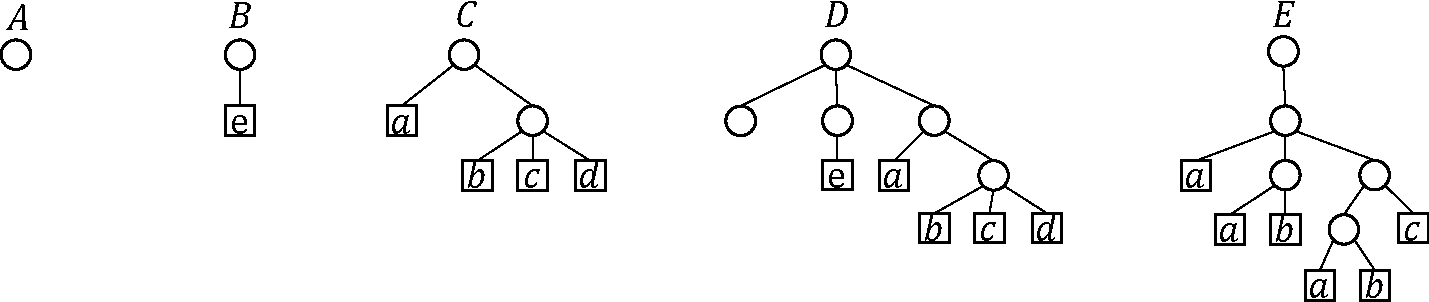
\includegraphics[width=0.8\textwidth]{./figure/pdf/cropped/GLGraph.pdf}
  \caption{广义表的图形表示}
  \label{fig:generalized_table}
\end{figure}

广义表 $GL$ 的表头为第一个元素 $a_1$,其余部分 $(a_2, \dots, a_i, \dots, a_n)$ 为 $GL$ 的表尾,分别记作 $\text{head}(GL) = a_1$ 和 $\text{tail}(GL) = (a_2, \dots, a_i, \dots, a_n)$。显然,一个广义表的表尾始终是一个广义表。空表无表头、表尾。这里仍取上面的示例:

\begin{itemize}
  \item $A$ 无表头、表尾;
  \item $\text{head}(B) = e$, $\text{tail}(B) = ()$;
  \item $\text{head}(C) = a$, $\text{tail}(C) = ((b, c, d))$;
  \item $\text{head}(D) = ()$, $\text{tail}(D) = ((e), (a, (b, c, d)))$;
  \item $\text{head}(E) = (a,(a,b),((a,b),c))$, $\text{tail}(E) = ()$。
\end{itemize}

其中,广义表 $A$ 和 $B$ 的深度为 1(注意广义表 $A$ 和广义表 $B$ 的深度相同,因为它们均只有一重括号),
广义表 $C, D, E$ 的深度分别为 2, 3 和 4。

\subsection{广义表的存储结构}

广义表是一种递归的数据结构,因此很难为每个广义表分配固定大小的存储空间,所以其存储结构只好采用链式存储结构。

从图\ref{fig:generalized_table_node} 中可以看到,广义表有两类结点,一类为圆圈结点,在这里对应子表;另一类为方形结点,在这里对应原子。

为了使子表和原子两类结点既能在形式上保持一致,又能进行区别,可采用以下结构形式:

\begin{figure}[!htbp]
  \centering
  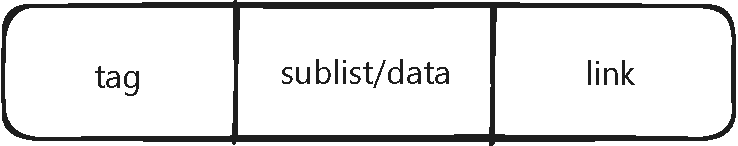
\includegraphics[width=0.5\textwidth]{./figure/pdf/cropped/GLStruct.pdf}
  \caption{广义表的存储结构}
  \label{fig:generalized_table_node}
\end{figure}

其中,$tag$ 为标志域,用于区分两类结点,即由 $tag$ 决定是使用结点的$sublist$ 域还是 $data$ 域:

\begin{itemize}
  \item 当 $tag = 0$ 时,表示该结点是原子结点,此时 $data$ 域存放原子值;
  \item 当 $tag = 1$ 时,表示该结点是子表结点,此时 $sublist$ 域存放指向子表的指针。
  \end{itemize}

  $link$ 域是指向下一个结点的指针,用于将广义表中的各个结点连接起来。当没有下一个结点时,$link$ 域为 $NULL$。

  例如前面的广义表$C$的存储结构如图\ref{fig:GLStructGraph}所示。

  \begin{figure}[!htbp]
    \centering
    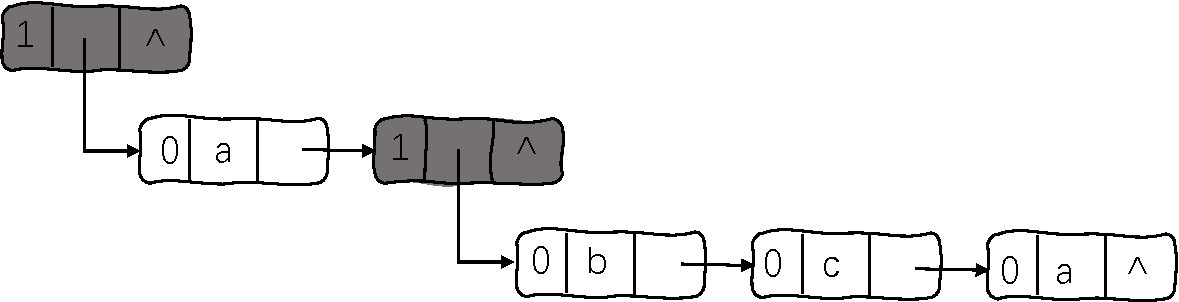
\includegraphics[width=0.8\textwidth]{./figure/pdf/cropped/GLStructGraph.pdf}
    \caption{广义表$C$的存储结构}
    \label{fig:GLStructGraph}
  \end{figure}


  采用C/C++语言的结构体定义广义表的存储结构如代码\ref{code:GLStruct}所示。

  \begin{lstlisting}[language=C++, caption={广义表的存储结构}, label={code:GLStruct}]
  typedef struct GLNode {
    int tag; // 标志域,0表示原子结点,1表示子表结点
    union {
      AtomType data; // 原子结点的值域,AtomType为原子结点的数据类型
      struct GLNode *sublist; // 子表结点的指针域,指向子表
    } val;
    struct GLNode *link; // 指向下一个结点的指针域
  } GLNode, *GList;
  \end{lstlisting}

\subsection{广义表的运算}

\subsubsection{广义表的创建}

广义表的创建是指根据广义表的逻辑结构,按照广义表的存储结构建立广义表的过程。广义表的创建可以采用递归的方法,即先创建子表,再创建广义表。

\begin{lstlisting}[language=C++, caption={广义表的创建}]
  void CreateGList(GList &L, char *s) {
    if (!*s) {
      L = NULL;
    } else {
      L = (GList)malloc(sizeof(GLNode));
      if (!L) {
        exit(OVERFLOW);
      }
      if (*s == '(') {
        L->tag = 1;
        CreateGList(L->val.sublist, s + 1);
      } else {
        L->tag = 0;
        L->val.data = *s;
      }
      CreateGList(L->link, s + 1);
    }
  }
\end{lstlisting}

\subsubsection{广义表的长度}

广义表的长度是指广义表中元素的个数。在广义表中,同一层次的每个结点是通过link域链接起来的,将其看成是带头结点的单链表,这样球广义表
的长度就是求单链表的长度。可以通过非递归的方法求得广义表的长度,即采用循环的方法,依次遍历广义表中的元素,统计广义表中元素的个数。

\begin{lstlisting}[language=C++, caption={广义表的长度}]
  int GListLength(GList *L){
    int len = 0;
    GLNode *gl;
    gl = L->val.sublist;
    while (gl) {
      len++;
      gl = gl->link;
    }
    return len;
  }
\end{lstlisting}

\subsubsection{广义表的深度}

对于广义表 $G$,其深度等于所有元素的最大深度加 1。若 $G$ 为原子,其深度为 0。求广义表深度的递归模型 $F(G)$ 如下:

\[
F(G) =
\begin{cases} 
0, & \text{若 } G \text{ 为原子} \\ 
1, & \text{若 } G \text{ 为空表} \\ 
\max \{F(\text{sub}(G))\} + 1, & \text{其他情况}
\end{cases}
\]

其中,$\text{sub}(G)$ 是 $G$ 的子表。

求广义表的深度的算法如下:

\begin{lstlisting}[language=C++, caption={广义表的深度}]
  int GListDepth(GList *L) {
    int max = 0;
    GLNode *gl;
    if(L->tag == 0) {// 原子结点
      return 0;// 原子结点的深度为 0
    }
    if (!L) {// 空表
      return 1;// 空表的深度为 1
    }
    gl = L->val.sublist;
    while (gl) {// 遍历广义表中的元素
      int depth = GListDepth(gl);
      if (depth > max) {
        max = depth;
      }
      gl = gl->link;
    }
    return max + 1;
  }
\end{lstlisting}


\subsubsection{输出广义表}

输出广义表是指将广义表中的元素按照广义表的逻辑结构输出。输出广义表的算法如下:

\begin{lstlisting}[language=C++, caption={输出广义表}]
  void PrintGList(GList *L) {
    if(!L) {//空表直接返回
      return;
    }
    GLNode *gl;
    if (L->tag == 0) {// 原子结点
      printf(``%c``, L->val.data);// 输出原子结点的值
    } else {// 子表结点
      printf(``(``);
      gl = L->val.sublist;
      while (gl) {
        PrintGList(gl);// 递归输出子表
        gl = gl->link;
        if (gl) {
          printf(``,``);
        }
      }
      printf(``)``);
    }
  }
\end{lstlisting}
\chapter{树}

\section{树的基本概念}

\subsection{树的定义}

\begin{itemize}
  \item 树是由 $n$ 个 ($n \geq 0$) 结点(或元素)组成的有限集合。
  \item 当 $n = 0$ 时,称作空树。
  \item 若 $n > 0$,在这 $n$ 个结点中有且仅有一个结点作为树的根结点,简称为根。
  \item 若 $n > 1$,除根结点以外的其他结点可分为 $m$ ($m \geq 0$) 个互不相交的有限集 $T_1, T_2, \dots, T_m$,其中每个子集本身又是一棵符合本定义的树,称为根结点的子树。
\end{itemize}

显然,树的定义是递归的,因为在树的定义中又用到了树的定义。树既是一种逻辑结构,它同时又是一种分层结构。
\subsection{树的逻辑表示方法}

\textbf{树形表示法 (tree representation)}:用一个圆圈表示一个结点,圆圈内的符号代表该结点的数据信息,结点之间的关系通过连线表示。虽然每条连线上都不带有箭头(即方向),但它仍然是有方向的,其方向隐含着从上向下,即连线的上方结点是下方结点的前驱结点,下方结点是上方结点的后继结点。它的直观形象是一棵倒置的树(树根在上,树叶在下),如图 7.1(a) 所示。

\textbf{说明}:在树形表示法中,尽管用没有箭头的连线表示结点之间的关系,但实际上树中结点之间的关系是一种有向关系。
例如,图\ref{fig:tree}中结点 $A$ 和 $B$ 之间的连线对应序偶 $\langle A, B \rangle$。

\begin{figure}[!htbp]
  \centering
  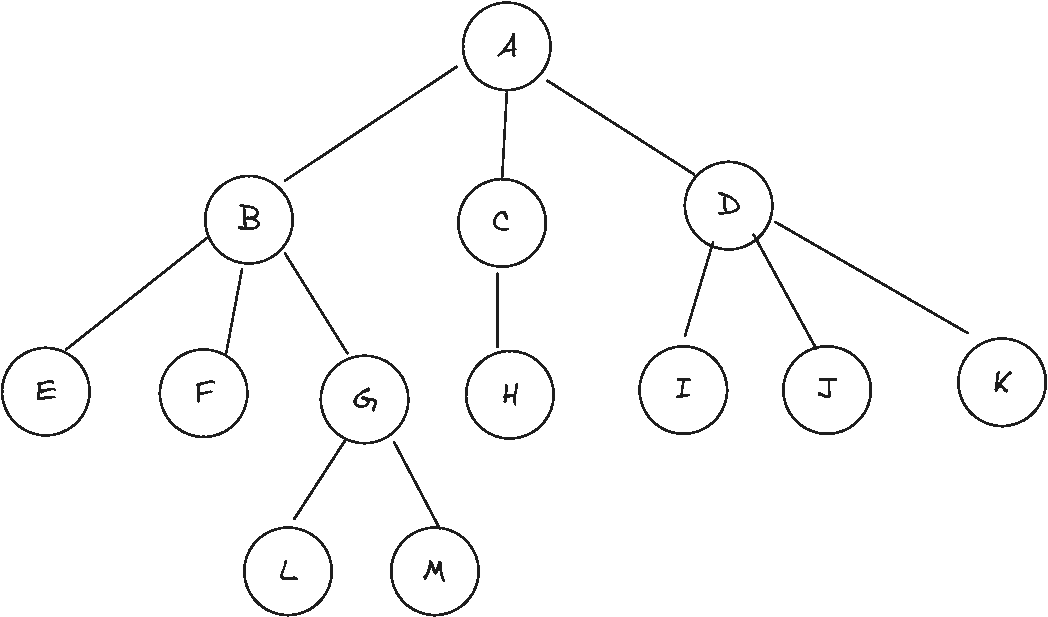
\includegraphics[width=0.8\textwidth]{./figure/pdf/cropped/tree.pdf}
  \caption{树的逻辑表示}
  \label{fig:tree}
\end{figure}
\subsection{树的基本术语}
下面介绍树的常用术语:

\begin{enumerate}
  \item \textbf{结点的度与树的度}:树中某个结点的子树的个数称为该结点的度(degree of node)。
  树中所有结点的度中的最大值称为树的度(degree of tree),通常将度为 $m$ 的树称为 $m$ 次树($m$-ary tree)。
  例如,图\ref{fig:tree} 是一棵 3 次树。

  \item \textbf{分支结点与叶子结点}:树中度不为零的结点称为非终端结点,又叫分支结点(branch)。
  度为零的结点称为叶子结点(leaf)。在分支结点中,每个结点的分支数就是该结点的度。如对于度为 1 的结点,其分支数为 1,
  被称为单分支结点;对于度为 2 的结点,其分支数为 2,被称为双分支结点,依此类推。例如,在图\ref{fig:tree}所示的树中,$B, C$ 和 $D$ 是分支结点,而 $E, F$ 和 $G$ 是叶子结点。

  \item \textbf{路径与路径长度}:对于树中的任意两个结点 $A$ 和 $B$,若树中存在一个结点序列 $(A_1, A_2, \dots, A_n)$ 
  使得序列中除 $A_1$ 和 $A_n$ 以外的任一结点都是其在序列中的前一个结点的后继结点,
  则称该结点序列为由 $A$ 到 $B$ 的一条路径(path)。路径长度(path length)是该路径所通过的结点数目减 1(即路径上分支数目)。
  显然,从树的根结点到树中其余结点均存在一条路径。例如,在图 \ref{fig:tree} 所示的树中,从 $A$ 到 $K$ 的路径为 $(A, D, I, K)$,其长度为 3,而 $(K, I, D, A)$ 为从 $K$ 到 $A$ 的逆路径。

  \item \textbf{孩子结点、双亲结点和兄弟结点}:在一棵树中,每个结点的后继结点被称为该结点的孩子结点(children)。相
  应地,该结点被称为孩子结点的双亲结点(parent)。具有同一双亲结点的孩子结点互为兄弟结点(sibling)。
  进一步推广这些关系,可以把每个结点对应子树中的所有结点(除自身外)称为该结点的子孙结点(descendant),
  把从根结点到达某个结点的路径上经过的所有结点(除自身外)称为该结点的祖先结点(ancestor)。例如,在图 \ref{fig:tree} 所示的树中,结点 $B, C, D$ 互为兄弟结点,结点 $D$ 的子孙结点有 $F, I, K, L$ 和 $M$,结点 $F$ 的祖先结点有 $A$ 和 $D$。

  \item \textbf{结点深度与树的高度}:结点深度(depth)是从树根开始定义的,根结点为第一层,它的孩子结点为第二层,
  依此类推,一个结点所在的层次为其双亲结点的层次加 1。树中结点的最大层次称为树的高度(height of tree)或树的深度(
  depth of tree)。

  \item \textbf{有序树和无序树}:若树中各结点的子树是按照一定的次序从左向右安排的,且相对次序是不能随意变换的,
  则称为有序树(ordered tree),否则称为无序树(unordered tree)。一般情况下,如果没有特别说明,默认树都是指有序树。

  \item \textbf{森林}:$m \ (m \geq 0)$ 个互不相交的树的集合称为森林(forest)。
  把含有多棵子树的树的根结点删去就成了森林(forest)。反之,给 $m \ (m \geq 1)$ 棵独立的树加上一个根结点,
  并把这 $m$ 棵树作为该结点的子树,则森林就变成了一棵树。
\end{enumerate}
\subsection{树的基本性质}

\begin{enumerate}
  \item \textbf{树中的结点数等于所有结点的度数加 1}:
  \begin{itemize}
    \item \textbf{证明}:不难想象,除根结点以外,每个结点有且仅有一个指向它的前驱结点。也就是说每个结点和指向它的分支一一对应。
    假设树中一共有 $b$ 个分支,那么除了根结点,整个树就包含有 $b$ 个结点,所以整个树的结点数就是这 $b$ 个结点加上根结点,设为 $n$,则 $n = b + 1$。而分支数 $b$ 也就是所有结点的度数,证毕。
  \end{itemize}

  \item \textbf{度为 $m$ 的树中第 $i$ 层上至多有 $m^{i-1}$ 个结点($i \geq 1$)}:
  \begin{itemize}
    \item \textbf{证明}(数学归纳法):
    \begin{itemize}
      \item 首先考虑 $i = 1$ 的情况:第一层只有根结点,即一个结点,$i = 1$ 带入式子满足。
      \item 假设第 $i-1$ 层满足这个性质,第 $i-1$ 层最多有 $m^{i-2}$ 个结点。
      \item 又因为树的度为 $m$,所以对于第 $i-1$ 层的每个结点,最多有 $m$ 个孩子结点。所以第 $i$ 层的结点数最多是第 $i-1$ 层的 $m$ 倍,所以第 $i$ 层上最多有 $m^{i-1}$ 个结点。
    \end{itemize}
  \end{itemize}

  \item \textbf{高度为 $h$ 的 $m$ 叉树至多有 $\frac{m^h - 1}{m - 1}$ 个结点}。

  \item \textbf{具有 $n$ 个结点的 $m$ 叉树的最小高度为 $\log_m(n(m-1)+1)$}。
\end{enumerate}


\section{二叉树}
二叉树是一个有限的结点集合,这个集合或者为空,或者由一个根结点和两棵互不相交的、分别称为根结点的左子树和右子树的二叉树组成。

\subsection{二叉树的定义}


\begin{itemize}
  \item 二叉树是 $n$ ($n \geq 0$) 个结点的有限集合:
  \begin{enumerate}
    \item 空二叉树,即 $n = 0$。
    \item 由一个根结点和两个互不相交的被称为根的左子树和右子树组成。左子树和右子树又分别是一棵二叉树。
  \end{enumerate}
  \item 二叉树的特点:
  \begin{enumerate}
    \item 每个结点最多有两棵子树。
    \item 左右子树有顺序,不能随意颠倒。
  \end{enumerate}
\end{itemize}

\textbf{二叉树与度为 2 的树的区别}

\begin{itemize}
  \item 度为 2 的树中至少有一个结点的度为 2,而二叉树没有这个要求。
  \item 度为 2 的树不区分左右子树,而二叉树严格区分左右子树。
\end{itemize}


二叉树的五种基本形态如图\ref{fig:binary_tree}所示:

\begin{itemize}
  \item \textbf{空二叉树}:没有任何结点的二叉树。
  \item \textbf{只有一个根结点}:只有一个根结点,没有左子树和右子树。
  \item \textbf{只有左子树}:只有左子树,没有右子树。
  \item \textbf{只有右子树}:只有右子树,没有左子树。
  \item \textbf{左右子树都有}:既有左子树,又有右子树。
\end{itemize}



\begin{figure}[!htbp]
  \centering
  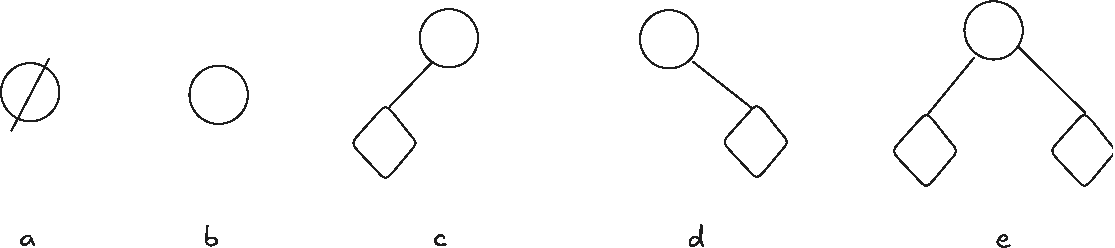
\includegraphics[width=0.8\textwidth]{./figure/pdf/cropped/fiveBTree.pdf}
  \caption{二叉树的五种基本形态}
  \label{fig:binary_tree}
\end{figure}




\subsection{特殊二叉树}

\subsubsection{满二叉树}

在一颗二叉树中,如果所有分支结点都存在左子树和右子树,并且所有叶子结点都在同一层上,这样的二叉树称为满二叉树。如图\ref{fig:full_binary_tree}所示。

\begin{figure}[!htbp]
  \centering
  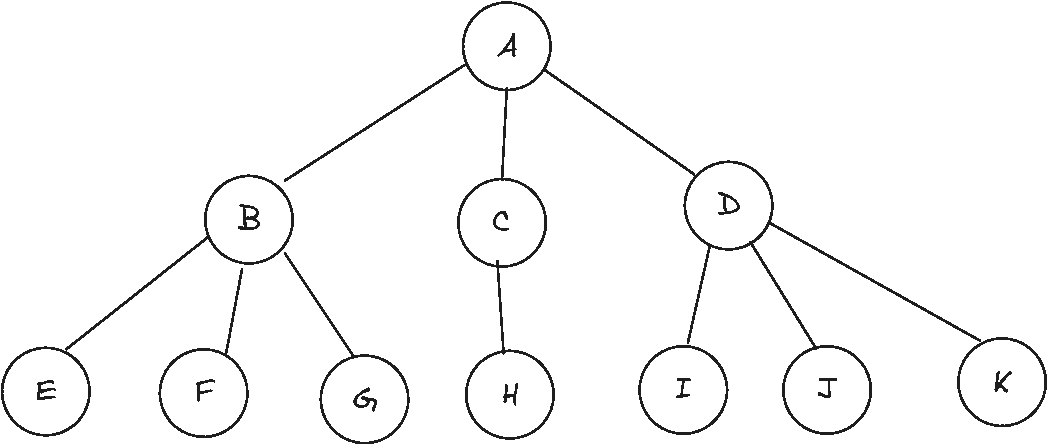
\includegraphics[width=0.8\textwidth]{./figure/pdf/cropped/fullBTree.pdf}
  \caption{满二叉树}
  \label{fig:full_binary_tree}
\end{figure}

非空满二叉树的特点如下:

\begin{itemize}
  \item 叶子结点只能出现在最下一层。
  \item 非叶子结点的度一定是 2。
  \item 在同样深度的二叉树中,满二叉树的结点个数最多,叶子数最多。
  \item 高度为 $h$ 的满二叉树,共有 $2^h - 1$ 个结点。
  \end{itemize}

\subsubsection{完全二叉树}

在一颗二叉树中,最多只有最下面的两层结点的度数可以小于 2,并且最下一层的结点都集中在该层最左边的若干位置上,这样的二叉树称为完全二叉树。如图\ref{fig:complete_binary_tree}所示。
如图\ref{fig:complete_binary_tree}所示。

\begin{figure}[!htbp]
  \centering
  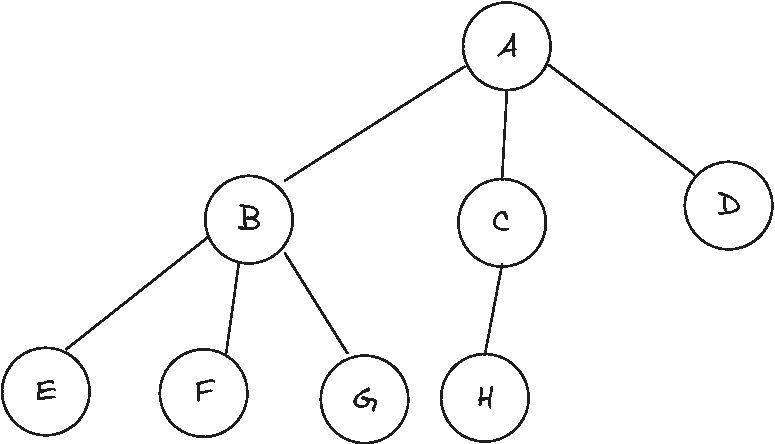
\includegraphics[width=0.6\textwidth]{./figure/pdf/cropped/comBTree.pdf}
  \caption{完全二叉树}
  \label{fig:complete_binary_tree}

\end{figure}


非空完全二叉树的特点如下:

\begin{itemize}
  \item 叶子结点只能出现在最下两层。
  \item 最下层的叶子结点都集中在该层最左边的若干位置上。
  \item 如果有度为 1 的结点,只可能有一个,且一定是最下层的最右边的结点。
  \item 按层序编号时,一旦出现编号为$i$的结点是叶子结点或只有左孩子,则编号为$i$的结点之后的结点必须都是叶子结点。
  \item 非叶子结点的度一定是 2。
  \item 在同样深度的二叉树中,完全二叉树的结点个数最多,叶子数最多。
  \item 高度为 $h$ 的完全二叉树,共有 $2^{h-1}$ 至 $2^h - 1$ 个结点。
  \item 当结点总数$n$为奇数时,$n_1 = 0$ ,为偶数时,$n_1 = 1$。
  \end{itemize}

\subsection{二叉树的性质}

二叉树相关性质如下:

\begin{enumerate}
  \item \textbf{非空二叉树上的叶子结点数等于度为 2 的结点数加 1}。
  \item \textbf{第 $i$ 层上的结点数最多为 $2^{i-1}$}。
  \item \textbf{深度为 $k$ 的二叉树至多有 $2^k - 1$ 个结点}。
  \item \textbf{对任何一棵非空二叉树 $T$,若 $n_0$ 表示叶子结点的个数,$n_1$ 表示度为 1 的结点个数,$n_2$ 表示度为 2 的结点个数,则 $n_0 = n_2 + 1$}。
  \item \textbf{具有 $n$ 个结点的完全二叉树的深度为 $\lfloor \log_2 n \rfloor + 1$}。
  \item \textbf{具有 $n$ 个结点的完全二叉树,从上到下、从左到右编号,对任意结点 $i$ 有}:
  \begin{itemize}
    \item \textbf{若 $i = 1$,则结点 $i$ 是二叉树的根结点,无双亲;}
    \item \textbf{若 $i > 1$,则其双亲是 $\lfloor i/2 \rfloor$;}
    \item \textbf{若 $2i \leq n$,则结点 $i$ 的左孩子是 $2i$;}
    \item \textbf{若 $2i + 1 \leq n$,则结点 $i$ 的右孩子是 $2i + 1$。}
  \end{itemize}
\end{enumerate}
\section{二叉树的存储结构}

\subsection{顺序存储结构}
二叉树的顺序存储结构就是用一组地址连续的存储单元来存放二叉树的数据元素,因此必须确定好树中各数据元素的存放次序,使得各数据元素在这个存放次序中的相互位置能反映出数据元素之间的逻辑关系。

对于完全二叉树和满二叉树,树中结点的层序编号可以唯一地反映出结点之间的逻辑关系,所以可以用一维数组按从上到下、从左到右的顺序存储树中的所有结点值,通过数组元素的下标关系反映完全二叉树或满二叉树中结点之间的逻辑关系。

例如,上图所示的完全二叉树对应的顺序存储结构如下图所示,编号为 $i$ 的结点值存放在数组下标为$i$的元素中(`\#` 表示空结点)。
由于 C/C++ 语言中的数组下标从 0 开始,这里为了一致性而没有使用下标为 0 的数组元素。

\begin{figure}[!htbp]
  \centering
  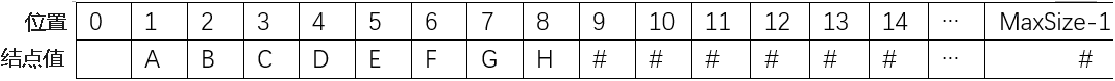
\includegraphics[width=0.8\textwidth]{./figure/pdf/cropped/seqBTree.pdf}
  \caption{完全二叉树的顺序存储结构}
  \label{fig:seq_binary_tree}
\end{figure}

显然,对于满二叉树和完全二叉树而言,这样的做法是十分方便的。但是如果是一般的二叉树,我们若还想让下标满足完全二叉树的特性,
就不得不增添许多的空结点,这就使得空间浪费严重。所以一般而言,对于一般二叉树采用下面介绍的链式存储方式。
\subsection{链式存储结构}

二叉树的链式存储结构是指用链表的方式存储二叉树。二叉树的链式存储结构是一种递归的定义方式,即二叉树是由结点构成的,
而结点又是由左右子树构成的。

二叉树链式存储结构的标准存储结构如图\ref{fig:binary_tree_node}所示,其中 $data$ 为结点的数据域,$lchild$ 和 $rchild$ 分别为结点的左孩子和右孩子指针域。

\begin{figure}[!htbp]
  \centering
  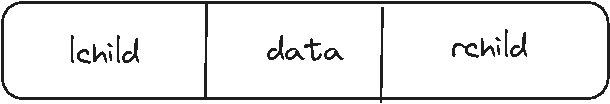
\includegraphics[width=0.5\textwidth]{./figure/pdf/cropped/BTreeStruct.pdf}
  \caption{二叉树的链式存储结构}
  \label{fig:binary_tree_node}
\end{figure}

二叉链中结点的定义如下:

\begin{lstlisting}[language=C++, caption={二叉树链式存储结构}]
  typedef struct BiTNode {
    TElemType data;
    struct BiTNode *lchild, *rchild;
  } BiTNode, *BiTree;
\end{lstlisting}

其中,$TElemType$ 为二叉树结点的数据类型,$BiTNode$ 为二叉树结点的结构体,$BiTree$ 为指向二叉树结点的指针。

由于本章后面的算法均用到二叉链存储结构,为此将其类型定义存储在头文件 $BiTree.h$ 中,方便后续的引用。

例如,图 \ref{fig:binary_tree_link}(左) 所示的二叉树的链式存储结构如图\ref{fig:binary_tree_link}(右)所示。

\begin{figure}[!htbp]
  \centering
  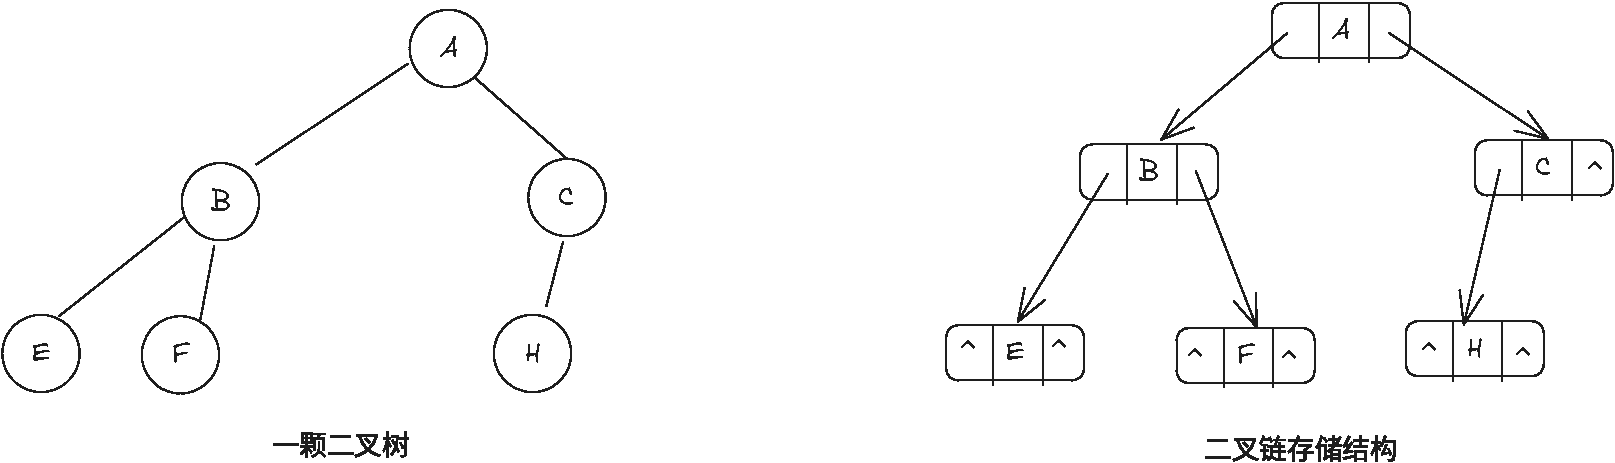
\includegraphics[width=0.8\textwidth]{./figure/pdf/cropped/BTreeGraph.pdf}
  \caption{二叉树的链式存储结构}
  \label{fig:binary_tree_link}
\end{figure}

\section{二叉树的遍历}


\subsection{遍历的定义}

二叉树的遍历是指按照一定的次序访问二叉树中的所有结点,并且每个结点仅被访问一次的过程。它是二叉树最基本的运算,是二叉树中所有其他运算实现的基础。

一棵二叉树由 3 个部分(即根结点、左子树和右子树)构成,可以从任何部分开始遍历,所以有 $3!$(即 6)种遍历方法。若规定子树的遍历总是先左后右(先右后左与之对称),
则对于非空二叉树,可得到以下 3 种递归的遍历方法,即先序遍历、中序遍历和后序遍历。另外,还有一种常见的层次遍历方法。

\subsection{递归遍历}

二叉树的递归遍历是指在遍历过程中,每个结点的左子树和右子树都是通过递归调用同一个遍历函数来实现的。具体又可分为先序遍历、中序遍历和后序遍历。我们将以图
\ref{fig:one_binary_tree_link}所示的二叉树为例,介绍这三种递归遍历方法。

\begin{figure}
  \centering
  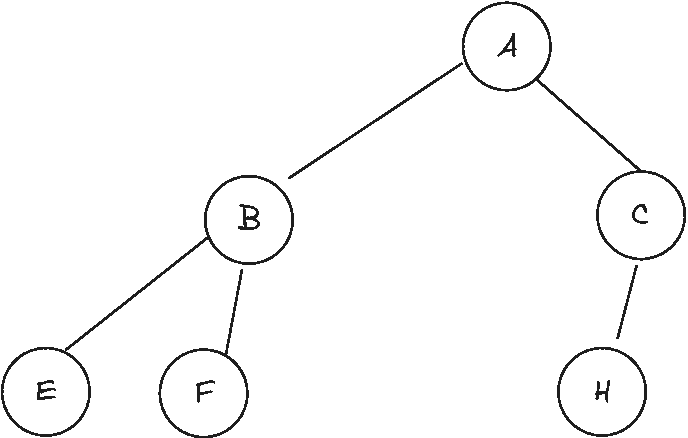
\includegraphics[width=0.5\textwidth]{./figure/pdf/cropped/oneBTree.pdf}
  \caption{二叉树的链式存储结构}
  \label{fig:one_binary_tree_link}
\end{figure}

\subsubsection{先序遍历}

先序遍历是指先访问根结点,然后依次先序遍历左子树和右子树。对于图\ref{fig:binary_tree_link}所示的二叉树,先序遍历的结果为 $ABEFCH$。

先序遍历的代码如\ref{code:precode}所示:


\begin{lstlisting}[language=C++, caption={先序遍历}, label={code:precode}]
  void PreOrderTraverse(BiTree T) {
    if (T == NULL) {
      return;
    }
    printf(``%c``, T->data);
    PreOrderTraverse(T->lchild);
    PreOrderTraverse(T->rchild);
  }
\end{lstlisting}

观察代码我们可以发现,先序遍历的过程就是先访问根结点,然后递归地先序遍历左子树和右子树。而对于递归而言,有两个关键点:

\begin{itemize}
  \item 递归的结束条件:对于二叉树的遍历,递归的结束条件就是当前结点为空。
  \item 递归的递推关系:对于先序遍历,递推关系就是先访问当前结点,然后递归地先序遍历左子树和右子树。
  \end{itemize}





\subsubsection{中序遍历}

中序遍历是指先中序遍历左子树,然后访问根结点,最后中序遍历右子树。对于图\ref{fig:binary_tree_link}所示的二叉树,中序遍历的结果为 $EBFAHC$。

中序遍历的代码如\ref{code:incode}所示:

\begin{lstlisting}[language=C++, caption={中序遍历}, label={code:incode}]
  void InOrderTraverse(BiTree T) {
    if (T == NULL) {
      return;
    }
    InOrderTraverse(T->lchild);
    printf(``%c``, T->data);
    InOrderTraverse(T->rchild);
  }

\end{lstlisting}

观察代码我们可以发现,中序遍历的过程就是先递归地中序遍历左子树,然后访问当前结点,最后递归地中序遍历右子树。
\subsubsection{后序遍历}


后序遍历是指先后序遍历左子树和右子树,然后访问根结点。对于图\ref{fig:binary_tree_link}所示的二叉树,后序遍历的结果为 $EFBHCA$。

后序遍历的代码如\ref{code:postcode}所示:

\begin{lstlisting}[language=C++, caption={后序遍历} , label={code:postcode}]
  void PostOrderTraverse(BiTree T) {
    if (T == NULL) {
      return;
    }
    PostOrderTraverse(T->lchild);
    PostOrderTraverse(T->rchild);
    printf(``%c``, T->data);
  }

\end{lstlisting}

观察代码我们可以发现,后序遍历的过程就是先递归地后序遍历左子树和右子树,然后访问当前结点。
\subsection{非递归遍历}

递归遍历的缺点是递归调用时需要保存函数调用信息,因此会占用较多的栈空间。为了解决这个问题,可以使用非递归遍历的方法。


\subsubsection{先序遍历}

由先序遍历过程可知,先访问根结点,再遍历左子树,最后遍历右子树。所以先访问根结点及其所有左下结点,但是因为在二叉链表中并没有指向双亲结点的指针,
所以我们需要将已访问过的结点存入栈中。此时栈顶结点要么没有左子树,要么左子树已遍历过,所以转向它的右子树,对右子树的处理与上述过程类似。

先序遍历的非递归算法如\ref{code:precode2}所示:

\begin{lstlisting}[language=C++, caption={先序遍历}, label={code:precode2}]
  void PreOrderTraverse(BiTree T) {
    InitStack(S);
    BiTree p = T;
    while (p != NULL || !StackEmpty(S)) {//栈不空或者p不空
      if (p != NULL) {//一直向左并将沿途结点压入栈
        printf(``%c``, p->data);//访问结点
        Push(S, p);
        p = p->lchild;
      } else {//结点弹出栈
        Pop(S, p);
        p = p->rchild;
      }
    }
  }
\end{lstlisting}

注:外循环中的条件是指针p不为空或者栈不为空,这是因为,p是指向当前所要访问元素,只要它不为空我们就要就行访问和入栈,当p一路向左直至为空的时候,
说明此时应该转头去访问双亲结点(如果有)的右子树了,
也就是这里我们要去判断栈是否为空,若不为空,我们便同样要进入循环,进行类似的操作。同学们对于这类较复杂的算法过程一定要手动进行模拟,不能光靠想。

先序遍历过程中指针和栈的变化如表\ref{tab:preorder_stack}所示。

\begin{table}[!htbp]
  \centering
  \caption{先序遍历过程中指针和栈的变化}
  \begin{tabular}{|c|c|c|c|}
  \hline
  \textbf{p指针的值} & \textbf{当前访问结点} & \textbf{当前栈的操作} & \textbf{当前栈内元素(栈底 $\to$ 栈顶)} \\ \hline
  A & A & A入栈 & A \\ \hline
  B & B & B入栈 & A B \\ \hline
  E & E & E入栈 & A B E \\ \hline
  NULL &  &  & A B E \\ \hline
  E &  & E出栈 & A B \\ \hline
  NULL &  &  & A B \\ \hline
  B &  & B出栈 & A \\ \hline
  F & F & F入栈 & A F \\ \hline
  NULL &  &  & A F \\ \hline
  F &  & F出栈 & A \\ \hline
  NULL &  &  & A \\ \hline
  A &  & A出栈 &  \\ \hline
  C & C & C入栈 & C \\ \hline
  H & H & H入栈 & C H \\ \hline
  ... & ... & ... & ... \\ \hline
  \end{tabular}
  \label{tab:preorder_stack}
  \end{table}
\subsubsection{中序遍历}
中序非递归算法是在前面先序遍历非递归算法的基础上修改的,中序遍历顺序是左子树 根结点 右子树 所以需要将根结点及其左下结点依次进栈,但还不能访问,
因为它的左子树没有遍历.当达到根结点的最左下结点时,它是中序序列的开始结点,也是栈顶节点,出栈并访问它,然后转向它的右子树,对右子树的处理与上述过程类似.

中序遍历的非递归算法如\ref{code:incode2}所示:

\begin{lstlisting}[language=C++, caption={中序遍历}, label={code:incode2}]
  void InOrderTraverse(BiTree T) {
    InitStack(S);
    BiTree p = T;
    while (p != NULL || !StackEmpty(S)) {
      if (p != NULL) {
        Push(S, p);
        p = p->lchild;
      } else {
        Pop(S, p);
        printf(``%c``, p->data);
        p = p->rchild;
      }
    }
  }
\end{lstlisting}

中序遍历过程中指针和栈的变化如表\ref{tab:inorder_stack}所示。

\begin{table}[!htbp]
  \centering
  \caption{中序遍历过程中指针和栈的变化}
  \begin{tabular}{|c|c|c|c|}
  \hline
  \textbf{p指针的值} & \textbf{当前访问结点} & \textbf{当前栈操作} & \textbf{当前栈内元素(栈底 $\to$ 栈顶)} \\ \hline
  A &  & A入栈 & A \\ \hline
  B &  & B入栈 & A B \\ \hline
  E &  & E入栈 & A B E \\ \hline
  NULL &  &  & A B E \\ \hline
  E & E & E出栈 & A B \\ \hline
  NULL &  &  & A B \\ \hline
  B & B & B出栈 & A \\ \hline
  F &  & F入栈 & A F \\ \hline
  NULL &  &  & A F \\ \hline
  F & F & F出栈 & A \\ \hline
  NULL &  &  & A \\ \hline
  A & A & A出栈 &  \\ \hline
  C &  & C入栈 & C \\ \hline
  H &  & H入栈 & C H \\ \hline
  NULL &  &  & C H \\ \hline
  H & H & H出栈 & C \\ \hline
  NULL &  &  & C \\ \hline
  C & C & C出栈 &  \\ \hline
  NULL &  &  & 程序结束 \\ \hline
  \end{tabular}
  \label{tab:inorder_stack}
  \end{table}



\subsubsection{后序遍历}

后序遍历的顺序是:先访问左子树,再访问右子树,最后访问根结点。为了实现这一顺序,我们需要先将根结点及其左下结点依次压入栈中。即使栈顶结点 $p$ 的左子树已经遍历完或为空,也不能立即访问结点 $p$,因为它的右子树还没有遍历。只有当结点 $p$ 的右子树也遍历完后,才能访问结点 $p$。因此,后序遍历的实现比前序和中序遍历更复杂,因为它有更多的条件限制。

\textbf{模拟遍历流程}

1. 首先将 $A, B, E$ 入栈,发现 $E$ 没有左孩子也没有右孩子,直接输出 $E$,然后将 $E$ 出栈。

2. 此时栈顶元素为 $B$,访问 $B$,发现 $B$ 有右孩子,将右孩子 $F$ 入栈。

3. $F$ 和 $E$ 类似,输出 $F$ 后将其出栈。

4. 栈顶元素仍为 $B$,但此时 $B$ 的右孩子已经被访问过了,所以直接输出 $B$。

5. 栈顶元素变为 $A$,$A$ 有右孩子且未被访问,将右孩子 $C$ 入栈。

6. 按照同样的逻辑,继续遍历,直到栈为空。

\textbf{需要解决的问题}

在后序遍历中,我们需要判断栈顶元素的右孩子是否已经被访问过。为了解决这个问题,可以在每次访问结点时,将当前结点标记存储起来。当退回到栈顶元素时,检查当前结点是否是栈顶元素的右孩子:

如果是,说明右子树已经被访问过,可以直接访问栈顶元素。

如果不是,说明右子树还未遍历,需要继续处理右子树。

通过这种方法,我们可以正确地实现后序遍历。

后序遍历的非递归算法如\ref{code:postcode2}所示:

\begin{lstlisting}[language=C++, caption={后序遍历}, label={code:postcode2}]
  void PostOrderTraverse(BiTree T) {
    InitStack(S);
    BiTree p = T;
    BiTree r = NULL;
    while (p != NULL || !StackEmpty(S)) {
      if (p != NULL) {
        Push(S, p);
        p = p->lchild;
      } else {
        GetTop(S, p);
        if (p->rchild != NULL && p->rchild != r) {
          p = p->rchild;
        } else {
          Pop(S, p);
          printf(``%c``, p->data);
          r = p;
          p = NULL;
        }
      }
    }
  }
\end{lstlisting}

后序遍历过程中指针和栈的变化如表\ref{tab:postorder_stack}所示。
\begin{table}[!htbp]
  \centering
  \caption{后序遍历过程中指针和栈的变化}
  \begin{tabular}{|c|c|c|c|c|}
  \hline
  \textbf{p指针的值} & \textbf{r指针的值} & \textbf{当前访问元素} & \textbf{当前栈操作} & \textbf{bottom $\to$ top} \\ \hline
  A & NULL &  & A入栈 & A \\ \hline
  B & NULL &  & B入栈 & AB \\ \hline
  E & NULL &  & E入栈 & ABE \\ \hline
  NULL & NULL &  &  & ABE \\ \hline
  E (没有右孩子) & NULL & E & E出栈 & AB \\ \hline
  NULL & E &  &  & AB \\ \hline
  B & E &  &  & AB \\ \hline
  F & E &  & F入栈 & ABF \\ \hline
  NULL & E &  &  & ABF \\ \hline
  F (没有右孩子) & F & F & F出栈 & AB \\ \hline
  B (右孩子与r同) & F & B & B出栈 & A \\ \hline
  A (右孩子不等于r,继续向右遍历) & B &  &  & A \\ \hline
  C & B &  & C入栈 & AC \\ \hline
  H & B &  & H入栈 & ACH \\ \hline
  NULL & B &  &  & ACH \\ \hline
  H (没有右孩子) & B & H & H出栈 & AC \\ \hline
  C (没有右孩子) & H & C & C出栈 & A \\ \hline
  A (右孩子与r同) & C & A & A出栈 & 程序结束 \\ \hline
  \end{tabular}
  \label{tab:postorder_stack}
  \end{table}
\subsection{层次遍历}

层次遍历是指按照从上到下、从左到右的顺序,依次访问二叉树中的每个结点。层次遍历需要借助队列来实现,其基本思想是:

\begin{itemize}
  \item 先将根结点入队。
  \item 当队列不为空时,执行以下操作:
  \begin{itemize}
    \item 将队头结点出队并访问。
    \item 将队头结点的左孩子入队。
  \end{itemize}
\end{itemize}

层次遍历的代码如\ref{code:levelcode}所示:

\begin{lstlisting}[language=C++, caption={层次遍历}, label={code:levelcode}]
  void LevelOrderTraverse(BiTree T) {
    InitQueue(Q);
    BiTree p;
    EnQueue(Q, T);
    while (!QueueEmpty(Q)) {
      DeQueue(Q, p);
      printf(``%c``, p->data);
      if (p->lchild != NULL) {
        EnQueue(Q, p->lchild);
      }
      if (p->rchild != NULL) {
        EnQueue(Q, p->rchild);
      }
    }
  }
\end{lstlisting}



\section{二叉树的基本运算及其实现}
二叉树的基本运算包括创建二叉树、清空二叉树、销毁二叉树、判断二叉树是否为空、求二叉树的深度、求二叉树的结点个数等。这些运算是二叉树的基本操作,也是其他运算的基础。
\subsection{二叉树的创建}

大家想想我们在手画一棵二叉树的步骤,是不是先画出根结点,然后画出分支,再画出其孩子结点。如此循环往复。其实,所有的算法代码都是我们实际问题的模拟。我们先画的是根结点,那么我们就采取先序遍历来创建一棵二叉树。

我们之前学习过先序遍历的递归代码,现在让我们看看如何将最基本的递归遍历代码改造为创建一棵二叉树的代码。

首先,先序遍历的代码如下:

\begin{lstlisting}[language=C++, caption={先序遍历}]
  void PreOrderTraverse(BiTree T) {
    if (T == NULL) {
      return;
    }
    printf(``%c``, T->data);
    PreOrderTraverse(T->lchild);
    PreOrderTraverse(T->rchild);
  }
\end{lstlisting}

首先,我们应该明确,创建一棵二叉树的过程就是根据先序遍历的顺序,依次输入结点的值,
当输入的值为某个特定值(例如 \texttt{\#})时,表示该结点为空。代码如~\ref{code:create} 所示。

\begin{lstlisting}[language=C++, caption={创建二叉树}, label={code:create}]
  void CreateBiTree(BiTree &T) {
    TElemType ch;
    scanf(``%c``, &ch);
    if (ch == '#') {
      T = NULL;
    } else {
      T = (BiTree)malloc(sizeof(BiTNode));
      if (!T) {
        exit(OVERFLOW);
      }
      T->data = ch;
      CreateBiTree(T->lchild);
      CreateBiTree(T->rchild);
    }
  }
\end{lstlisting}

代码中,我们首先输入一个字符,如果该字符为 \texttt{\#},则表示该结点为空,否则我们为该结点分配内存空间,并将该字符赋值给该结点的数据域。接着,我们递归地创建左子树和右子树。

\subsection{二叉树的销毁}

二叉树的销毁是指将二叉树中的所有结点释放掉,使其成为一个空树。销毁二叉树的代码如\ref{code:destroy}所示。

\begin{lstlisting}[language=C++, caption={销毁二叉树}, label={code:destroy}]
  void DestroyBiTree(BiTree &T) {
    if (T == NULL) {
      return;
    }
    DestroyBiTree(T->lchild);
    DestroyBiTree(T->rchild);
    free(T);
    T = NULL;
  }
\end{lstlisting}

销毁二叉树的过程就是递归地销毁左子树和右子树,然后释放根结点的内存空间。

\subsection{二叉树的清空}

二叉树的清空是指将二叉树中的所有结点清空,使其成为一个空树。清空二叉树的代码如\ref{code:clear}所示。

\begin{lstlisting}[language=C++, caption={清空二叉树}, label={code:clear}]
  void ClearBiTree(BiTree &T) {
    if (T == NULL) {
      return;
    }
    ClearBiTree(T->lchild);
    ClearBiTree(T->rchild);
    T = NULL;
  }

\end{lstlisting}

清空二叉树的过程就是递归地清空左子树和右子树,然后将根结点置为空。

\subsection{二叉树的判空}

二叉树的判空是指判断二叉树是否为空。判空的代码如\ref{code:empty}所示。

\begin{lstlisting}[language=C++, caption={判空}, label={code:empty}]
  Status BiTreeEmpty(BiTree T) {
    if (T == NULL) {
      return TRUE;
    } else {
      return FALSE;
    }
  }

\end{lstlisting}

判空的过程就是判断根结点是否为空。

\subsection{二叉树的深度}

二叉树的深度是指二叉树中结点的最大层次。求二叉树的深度的代码如\ref{code:depth}所示。

\begin{lstlisting}[language=C++, caption={求深度}, label={code:depth}]
  int BiTreeDepth(BiTree T) {
    if (T == NULL) {
      return 0;
    }
    int ldepth = BiTreeDepth(T->lchild);
    int rdepth = BiTreeDepth(T->rchild);
    return ldepth > rdepth ? ldepth + 1 : rdepth + 1;
  }

\end{lstlisting}

求深度的过程就是递归地求左子树和右子树的深度,然后取两者中的较大值加 1。

\subsection{二叉树的结点个数}

二叉树的结点个数是指二叉树中结点的个数。求二叉树的结点个数的代码如\ref{code:count}所示。

\begin{lstlisting}[language=C++, caption={求结点个数}, label={code:count}]
  int BiTreeCount(BiTree T) {
    if (T == NULL) {
      return 0;
    }
    return BiTreeCount(T->lchild) + BiTreeCount(T->rchild) + 1;
  }

\end{lstlisting}

求结点个数的过程就是递归地求左子树和右子树的结点个数,然后将两者相加并加 1。

\subsection{求结点值为x的层次}

求结点值为 $x$ 的层次是指求出二叉树中值为 $x$ 的结点所在的层次。求结点值为 $x$ 的层次的代码如\ref{code:level}所示。

\begin{lstlisting}[language=C++, caption={求结点值为x的层次}, label={code:level}]
  int BiTreeLevel(BiTree T, TElemType x) {
    if (T == NULL) {
      return 0;
    }
    if (T->data == x) {
      return 1;
    }
    int llevel = BiTreeLevel(T->lchild, x);
    int rlevel = BiTreeLevel(T->rchild, x);
    if (llevel > 0) {
      return llevel + 1;
    } else if (rlevel > 0) {
      return rlevel + 1;
    } else {
      return 0;
    }
  }

\end{lstlisting}

求结点值为 $x$ 的层次的过程就是递归地求左子树和右子树中值为 $x$ 的结点所在的层次,然后取两者中的较大值加 1。


\section{二叉树的构造}

我们在这个小节中,将介绍二叉树的构造方法,包括根据先序遍历和中序遍历构造二叉树、根据中序遍历和后序遍历构造二叉树、根据层次遍历构造二叉树等。

我们假设二叉树的每个结点的值为单个字符,且不重复。同一颗二叉树具有唯一的先序遍历、中序遍历和后序遍历序列,但不同的二叉树可能具有相同的先序遍历、中序遍历和后序遍历序列。

如图\ref{fig:samePre}所示,5颗不同的二叉树具有相同的先序遍历序列 $ABC$

\begin{figure}[!htbp]
  \centering
  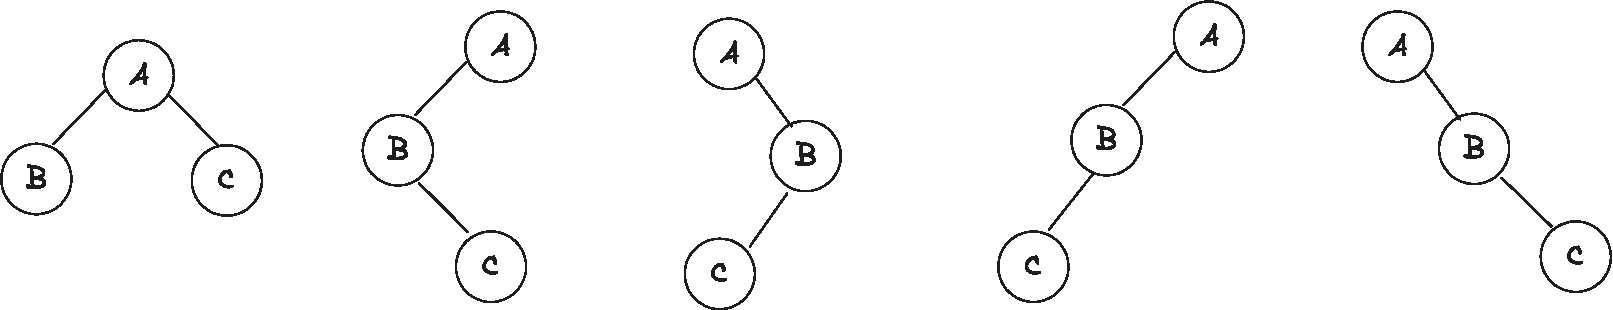
\includegraphics[width=0.8\textwidth]{./figure/fix/pdf/preBTree.pdf}
  \caption{具有相同先序遍历序列的不同二叉树}
  \label{fig:samePre}
\end{figure}

% \begin{figure}[!htbp]
%   \centering
%   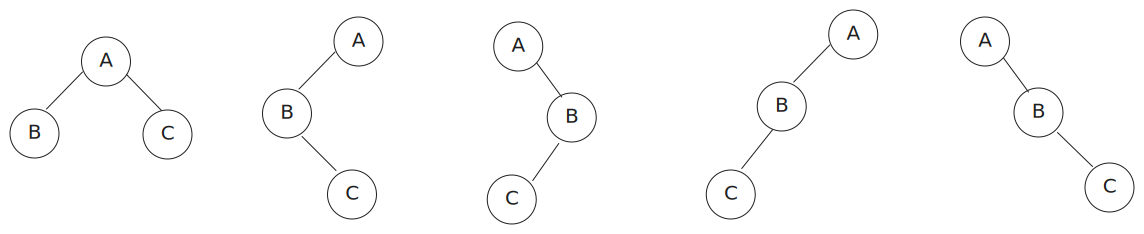
\includegraphics[width=0.8\textwidth]{./figure/fix/preBTree.svg}
%   \caption{具有相同先序遍历序列的不同二叉树}
%   \label{fig:samePre}
% \end{figure}

如图\ref{fig:sameIn}所示,5颗不同的二叉树具有相同的中序遍历序列 $ACB$

\begin{figure}[!htbp]
  \centering
  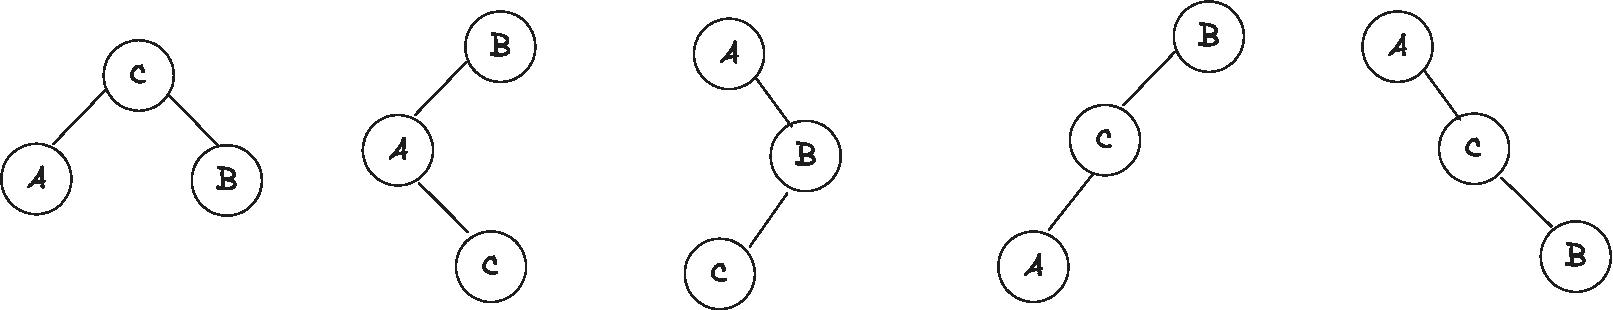
\includegraphics[width=0.8\textwidth]{./figure/fix/pdf/inBTree.pdf}
  \caption{具有相同中序遍历序列的不同二叉树}
  \label{fig:sameIn}
\end{figure}

如图\ref{fig:samePost}所示,5颗不同的二叉树具有相同的后序遍历序列 $CBA$

\begin{figure}[!htbp]
  \centering
  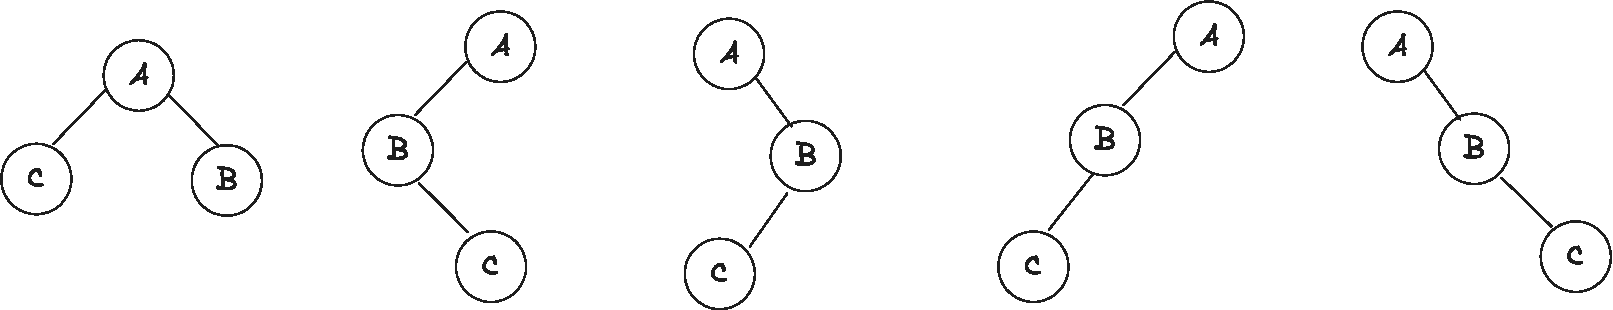
\includegraphics[width=0.8\textwidth]{./figure/fix/pdf/postBTree.pdf}
  \caption{具有相同后序遍历序列的不同二叉树}
  \label{fig:samePost}
\end{figure}

\subsection{根据先序遍历和中序遍历构造二叉树}

根据先序遍历和中序遍历构造二叉树的基本思想是:

\begin{itemize}
  \item 先序遍历序列的第一个结点为根结点。
  \item 在中序遍历序列中找到根结点,根结点左边的结点为左子树的中序遍历序列,根结点右边的结点为右子树的中序遍历序列。
  \item 根据左子树的中序遍历序列和先序遍历序列,递归地构造左子树。
  \item 根据右子树的中序遍历序列和先序遍历序列,递归地构造右子树。
  \end{itemize}

根据先序遍历和中序遍历构造二叉树的过程如图\ref{fig:preIn}所示。

\begin{figure}[!htbp]
  \centering
  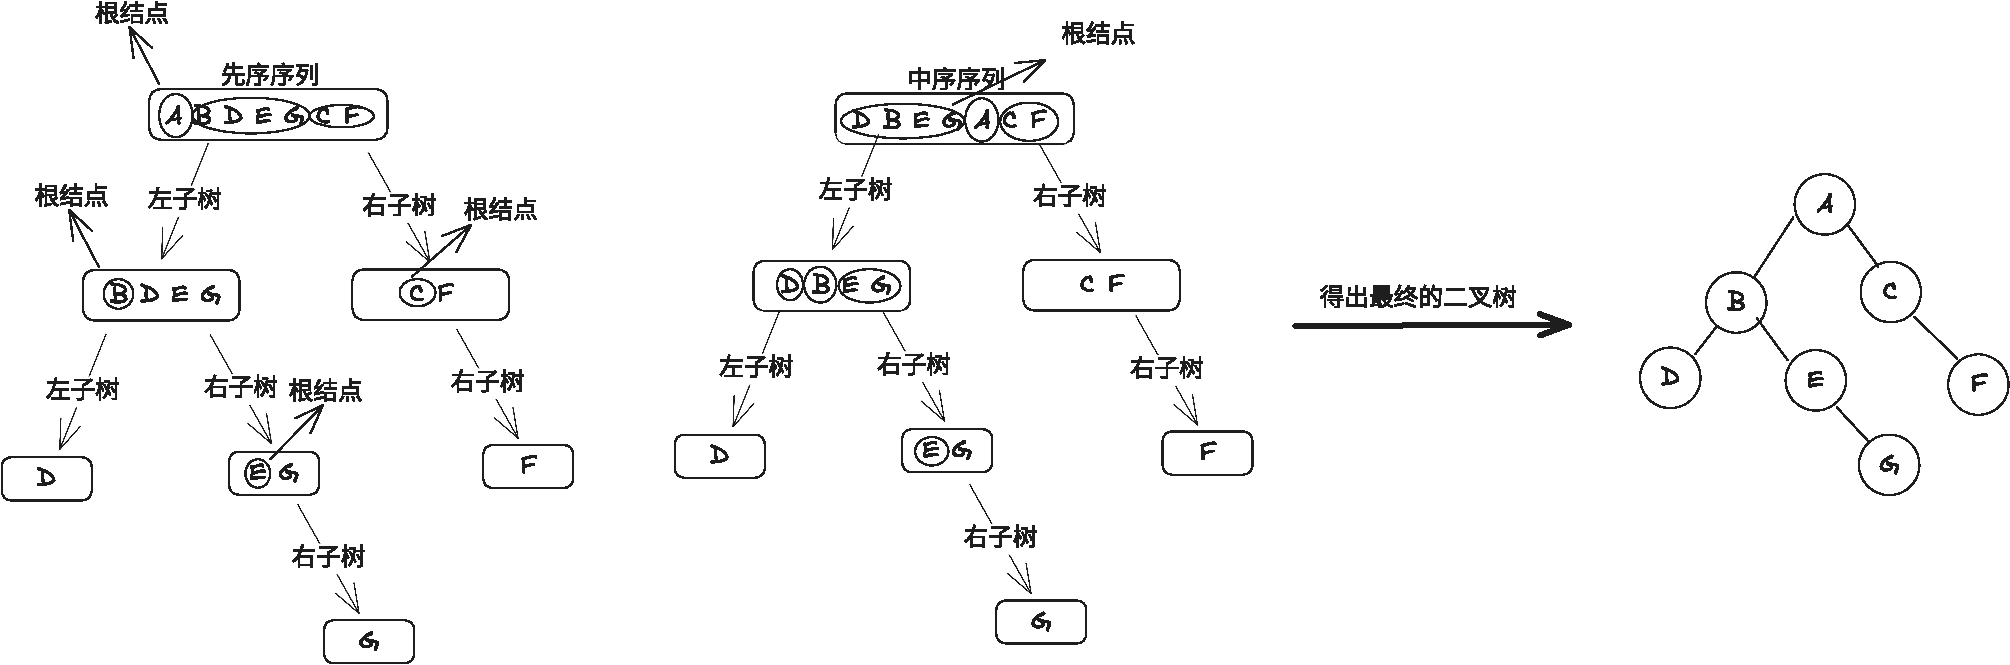
\includegraphics[width=0.8\textwidth]{./figure/fix/pdf/preAndIn.pdf}
  \caption{根据先序遍历和中序遍历构造二叉树}
  \label{fig:preIn}
\end{figure}

根据先序遍历和中序遍历构造二叉树的代码如\ref{code:preIn}所示。

\begin{lstlisting}[language=C++, caption={根据先序遍历和中序遍历构造二叉树}, label={code:preIn}]
  BiTree PreInCreateBiTree(TElemType *pre, TElemType *in, int n) {
    if (n == 0) {
      return NULL;
    }
    BiTree T = (BiTree)malloc(sizeof(BiTNode));
    if (!T) {
      exit(OVERFLOW);
    }
    T->data = *pre;
    int k = 0;
    while (in[k] != *pre) {
      k++;
    }
    T->lchild = PreInCreateBiTree(pre + 1, in, k);
    T->rchild = PreInCreateBiTree(pre + k + 1, in + k + 1, n - k - 1);
    return T;
  }
\end{lstlisting}

代码中,我们首先判断结点个数是否为 0,如果为 0,则返回空树。然后,我们为根结点分配内存空间,并将先序遍历序列的第一个结点赋值给根结点的数据域。接着,我们在中序遍历序列中找到根结点,根结点左边的结点为左子树的中序遍历序列,根结点右边的结点为右子树的中序遍历序列。然后,我们递归地构造左子树和右子树。

\section{线索二叉树}

对于具有 $n$ 个结点的二叉树,当采用二叉链存储结构时,每个结点有两个指针域,总共有 $2n$ 个指针域。又由于只有 $n-1$ 个结点被有效指针域所指向($n$ 个结点中只有根结点没有被有效指针域指向),则共有 $2n - (n-1) = n+1$ 个空链域。

遍历二叉树的结果是一个结点的线性序列,可以利用这些空链域存放指向结点的前驱结点和后继结点的地址。其规定是当某结点的左指针为空时,令该指针指向这个线性序列中该结点的前驱结点;当某结点的右指针为空时,令该指针指向这个线性序列中该结点的后继结点。这样的指向该线性序列中的“前驱结点”和“后继结点”的指针称为线索(thread)。

创建线索的过程称为线索化。线索化的二叉树称为线索二叉树(threaded binary-tree)。

由于遍历方式不同,产生的遍历线性序列也不同,会得到相应的线索二叉树。一般有先序线索二叉树、中序线索二叉树和后序线索二叉树。创建线索二叉树的目的是提高该遍历过程的效率。

那么,在线索二叉树中如何区分左指针指向的是左孩子结点还是前驱结点,右指针指向的是右孩子结点还是后继结点呢?为此,在结点的存储结构上增加两个标志位来区分这两种情况:

\begin{itemize}
  \item 左标志 $ltag$:
  \begin{itemize}
    \item $0$ 表示 $lchild$ 指向左孩子结点;
    \item $1$ 表示 $lchild$ 指向前驱结点。
  \end{itemize}
  \item 右标志 $rtag$:
  \begin{itemize}
    \item $0$ 表示 $rchild$ 指向右孩子结点;
    \item $1$ 表示 $rchild$ 指向后继结点。
  \end{itemize}
\end{itemize}

这样,每个结点的存储结构如下:

\[
\begin{array}{|c|c|c|c|c|}
\hline
\text{ltag} & \text{lchild} & \text{data} & \text{rchild} & \text{rtag} \\
\hline
\end{array}
\]

在某遍历方式的线索二叉树中,若开始结点 $p$ 没有左孩子,将 $p$ 结点的左指针改为线索,其左指针仍为空;若最后结点 $q$ 没有右孩子,将 $q$ 结点的右指针改为线索,其右指针仍为空。对于其他结点 $x$,若它没有左孩子,将左指针改为指向前驱结点的非空线索;若它没有右孩子,将右指针改为指向后继结点的非空线索。

为使创建线索二叉树的算法设计方便,在线索二叉树中再增加一个头结点。头结点的 $data$ 域为空;$lchild$ 指向无线索时的根结点,$ltag$ 为 $0$;$rchild$ 指向按某种方式遍历二叉树时的最后一个结点,$rtag$ 为 $1$。

图\ref{fig:threadedBTree}所示的线索二叉树,其中:
\begin{itemize}
  \item 图\ref{fig:threadedBTree}(a) 是二叉树(中序序列为 $D, B, G, A, E, C, F$);
  \item 图\ref{fig:threadedBTree}(c) 是中序线索二叉树(中序序列为 $D, G, B, A, E, C, F$);
  \item 图\ref{fig:threadedBTree}(b) 是先序线索二叉树(先序序列为 $A, B, D, G, C, E, F$);
  \item 图\ref{fig:threadedBTree}(d) 是后序线索二叉树(后序序列为 $G, D, B, E, F, C, A$)。
\end{itemize}
\begin{figure}[!htbp]
  \centering
  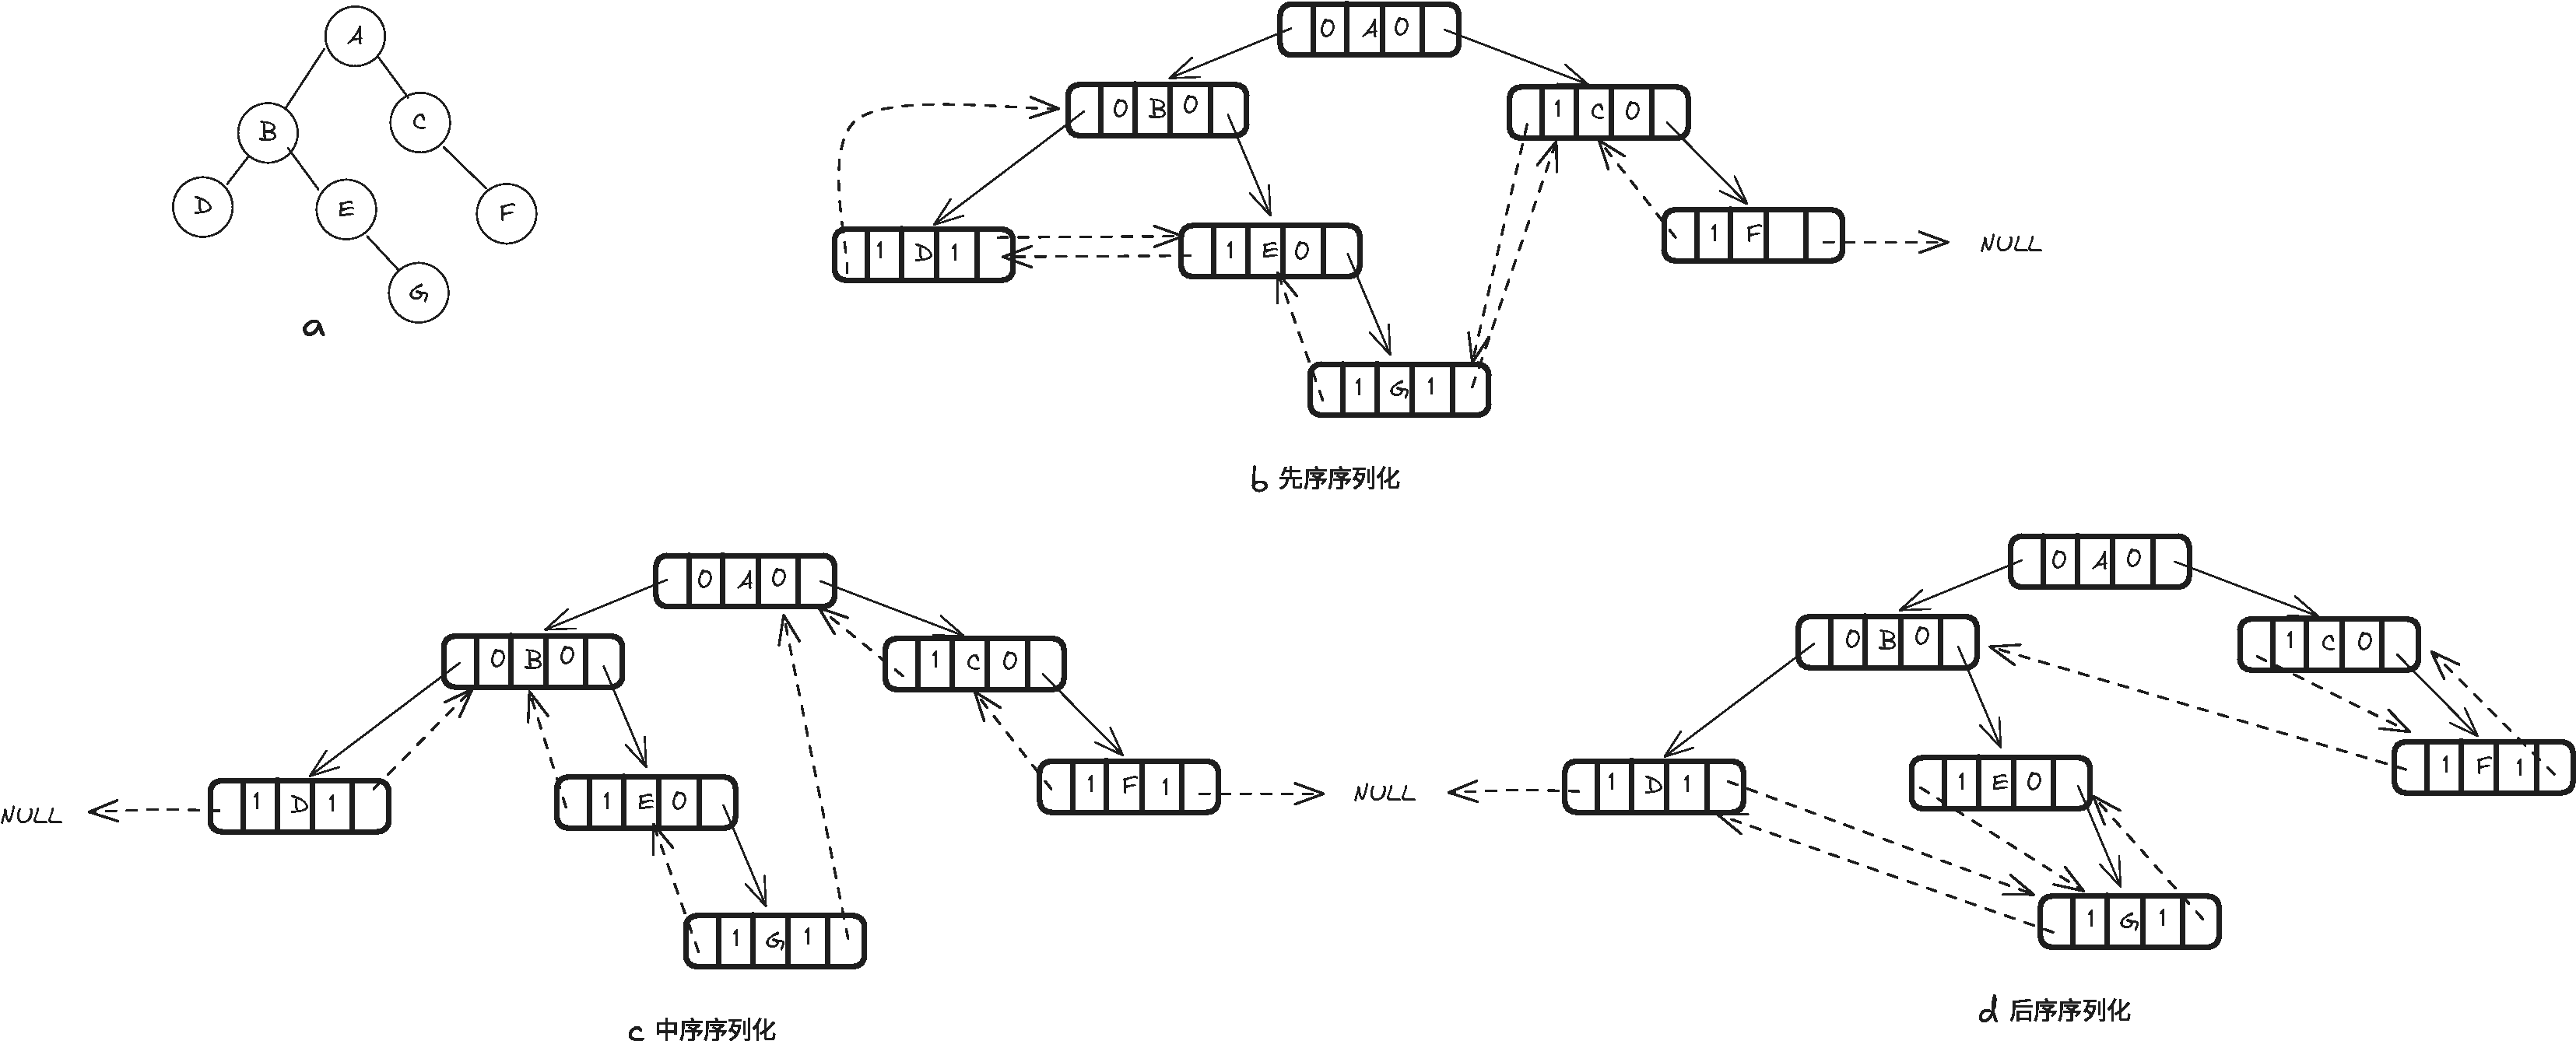
\includegraphics[width=1\textwidth]{./figure/pdf/cropped/threadBTree.pdf}
  \caption{线索二叉树}
  \label{fig:threadedBTree}
\end{figure}
图中的实线表示二叉树原来指针所指的结点,虚线表示线索二叉树所添加的线索。

\subsection{建立线索二叉树}

建立线索二叉树的过程是在遍历二叉树的过程中,将空指针域改为指向前驱结点或后继结点的线索。为了实现线索二叉树,将前面的二叉树的存储结构中的 $ltag$ 和 $rtag$ 
增加到结点中,同时增加一个头结点,头结点的 $lchild$ 指向根结点,$rchild$ 指向最后一个结点。其类型声明如下:

\begin{lstlisting}[language=C++, caption={线索二叉树结点类型定义}]
  typedef struct BiThrNode {
    TElemType data;
    struct BiThrNode *lchild, *rchild;
    int ltag, rtag;
  } BiThrNode, *BiThrTree;
\end{lstlisting}

线索二叉树的建立过程如下:

\begin{itemize}
  \item 若二叉树为空,则线索二叉树为空;
  \item 若二叉树不为空,则按照中序遍历的顺序,将二叉树中的每个结点的 $lchild$ 指针指向其前驱结点,$rchild$ 指针指向其后继结点。
  \end{itemize}

\subsection{中序线索化}

下面以中序线索二叉树为例讨论建立线索二叉树的算法。

\textbf{CreateThread(b)} 算法的功能是将以二叉链存储的二叉树 $T$ 进行中序线索化,并返回线索化后头结点的指针 $root$。\textbf{Thread(p)} 算法的功能是对
以结点 $p$ 为根的二叉树进行中序线索化。在整个算法中,$p$ 总是指向当前被线索化的结点,而 $pre$ 作为全局变量,指向刚访问过的结点。结点 $pre$ 是结点 $p$ 的
前驱结点,结点 $p$ 是结点 $pre$ 的后继结点。

\textbf{CreateThread(b)} 算法的思路如下:
1. 先创建头结点 $root$,其 $lchild$ 域为链指针,$rchild$ 域为线索。
2. 将 $lchild$ 指针指向根结点 $T$,如果 $T$ 为空,则将其 $lchild$ 指向自身;否则将 $root$ 的 $lchild$ 指向结点 $T$。
3. 初始化 $p$ 指向根结点,$pre$ 指向头结点 $root$。
4. 调用 \textbf{Thread(p)} 对整个二叉树进行线索化。
5. 最后加入指向头结点的线索,并将头结点的 $rchild$ 指针域线索化为指向最后一个结点(由于线索化直到 $p = NULL$ 为止,所以最后访问的结点是 $pre$)。

\textbf{Thread(p)} 算法类似于中序遍历的递归算法。在中序遍历中,$p$ 指向当前访问的结点,$pre$ 指向中序遍历的前一个结点(初始时,$pre$ 指向中
序线索二叉树的头结点 $root$)。若结点 $p$ 原来的左指针为空,则改为指向结点 $pre$ 的左线索;若结点 $pre$ 原来的右指针为空,则改为指向结点 $p$ 的右线索。

如代码\ref{code:threadIn}所示,中序线索二叉树的算法如下:

\begin{lstlisting}[language=C++, caption={中序线索化}, label={code:threadIn}]
  \begin{lstlisting}[language=C++, caption={中序线索化}]
  void CreateThread(BiThrTree &root, BiThrTree T) {//中序线索化
    root = (BiThrTree)malloc(sizeof(BiThrNode));//创建头结点
    if (!root) {
      exit(OVERFLOW);
    }
    root->ltag = 0;//头结点左标志为0
    root->rtag = 0;//头结点右标志为0
    root->rchild = root;
    if (!T) {
      root->lchild = root;
    } else {
      root->lchild = T;
      BiThrTree pre = root;
      Thread(T, pre);
      pre->rchild = root;
      pre->rtag = 1;//最后一个结点的右标志为1
      root->rchild = pre;
    }
  }
  
  void Thread(BiThrTree p, BiThrTree &pre) {
    if (p) {
      Thread(p->lchild, pre);
      if (!p->lchild) {
        p->lchild = pre;
        p->ltag = 1;
      }
      if (!pre->rchild) {
        pre->rchild = p;
        pre->rtag = 1;
      }
      pre = p;
      Thread(p->rchild, pre);
    }
  }
  \end{lstlisting}

\subsection{中序线索二叉树的遍历}

中序线索二叉树的遍历是指按照中序遍历的顺序访问中序线索二叉树中的每个结点。中序线索二叉树的中序遍历过程如下:

\begin{itemize}
  \item 从头结点开始,找到中序遍历的第一个结点,即最左下的结点;
  \item 依次访问结点的左孩子,直到遇到线索,输出该结点;
  \item 访问结点的右孩子,直到遇到线索,输出该结点;
  \item 重复上述过程,直到遇到头结点。
  \end{itemize}

中序线索二叉树的中序遍历代码如\ref{code:inThread}所示。

\begin{lstlisting}[language=C++, caption={中序线索二叉树的中序遍历}, label={code:inThread}]
  void InOrderTraverse_Thr(BiThrTree T) {
    BiThrTree p = T->lchild;
    while (p != T) {
      while (p->ltag == 0) {
        p = p->lchild;
      }
      printf(``%c``, p->data);
      while (p->rtag == 1 && p->rchild != T) {
        p = p->rchild;
        printf(``%c``, p->data);
      }
      p = p->rchild;
    }
  }

\end{lstlisting}

显然,该算法是非递归的,其中也没有使用到栈。尽管时间复杂度为 $O(n)$,但是该算法的空间复杂度为 $O(1)$,是一种非常高效的算法。
\section{树、森林和二叉树的转换}

\subsection{二叉树和树的转换}

将一颗树转换成二叉树的过程如下:
\begin{enumerate}
  \item 树中所有相邻兄弟之间加一条连线;
  \item 对树中的每个结点只保留它与长子之间的连线,删除与其他孩子之间的连线;
  \item 以树的根结点为轴心,将整棵树顺时针转动 $45^\circ$,使之结构层次分明。
\end{enumerate}

如图\ref{fig:tree2BiTree}所示,将树转换成二叉树的过程。

\begin{figure}[!htbp]
  \centering
  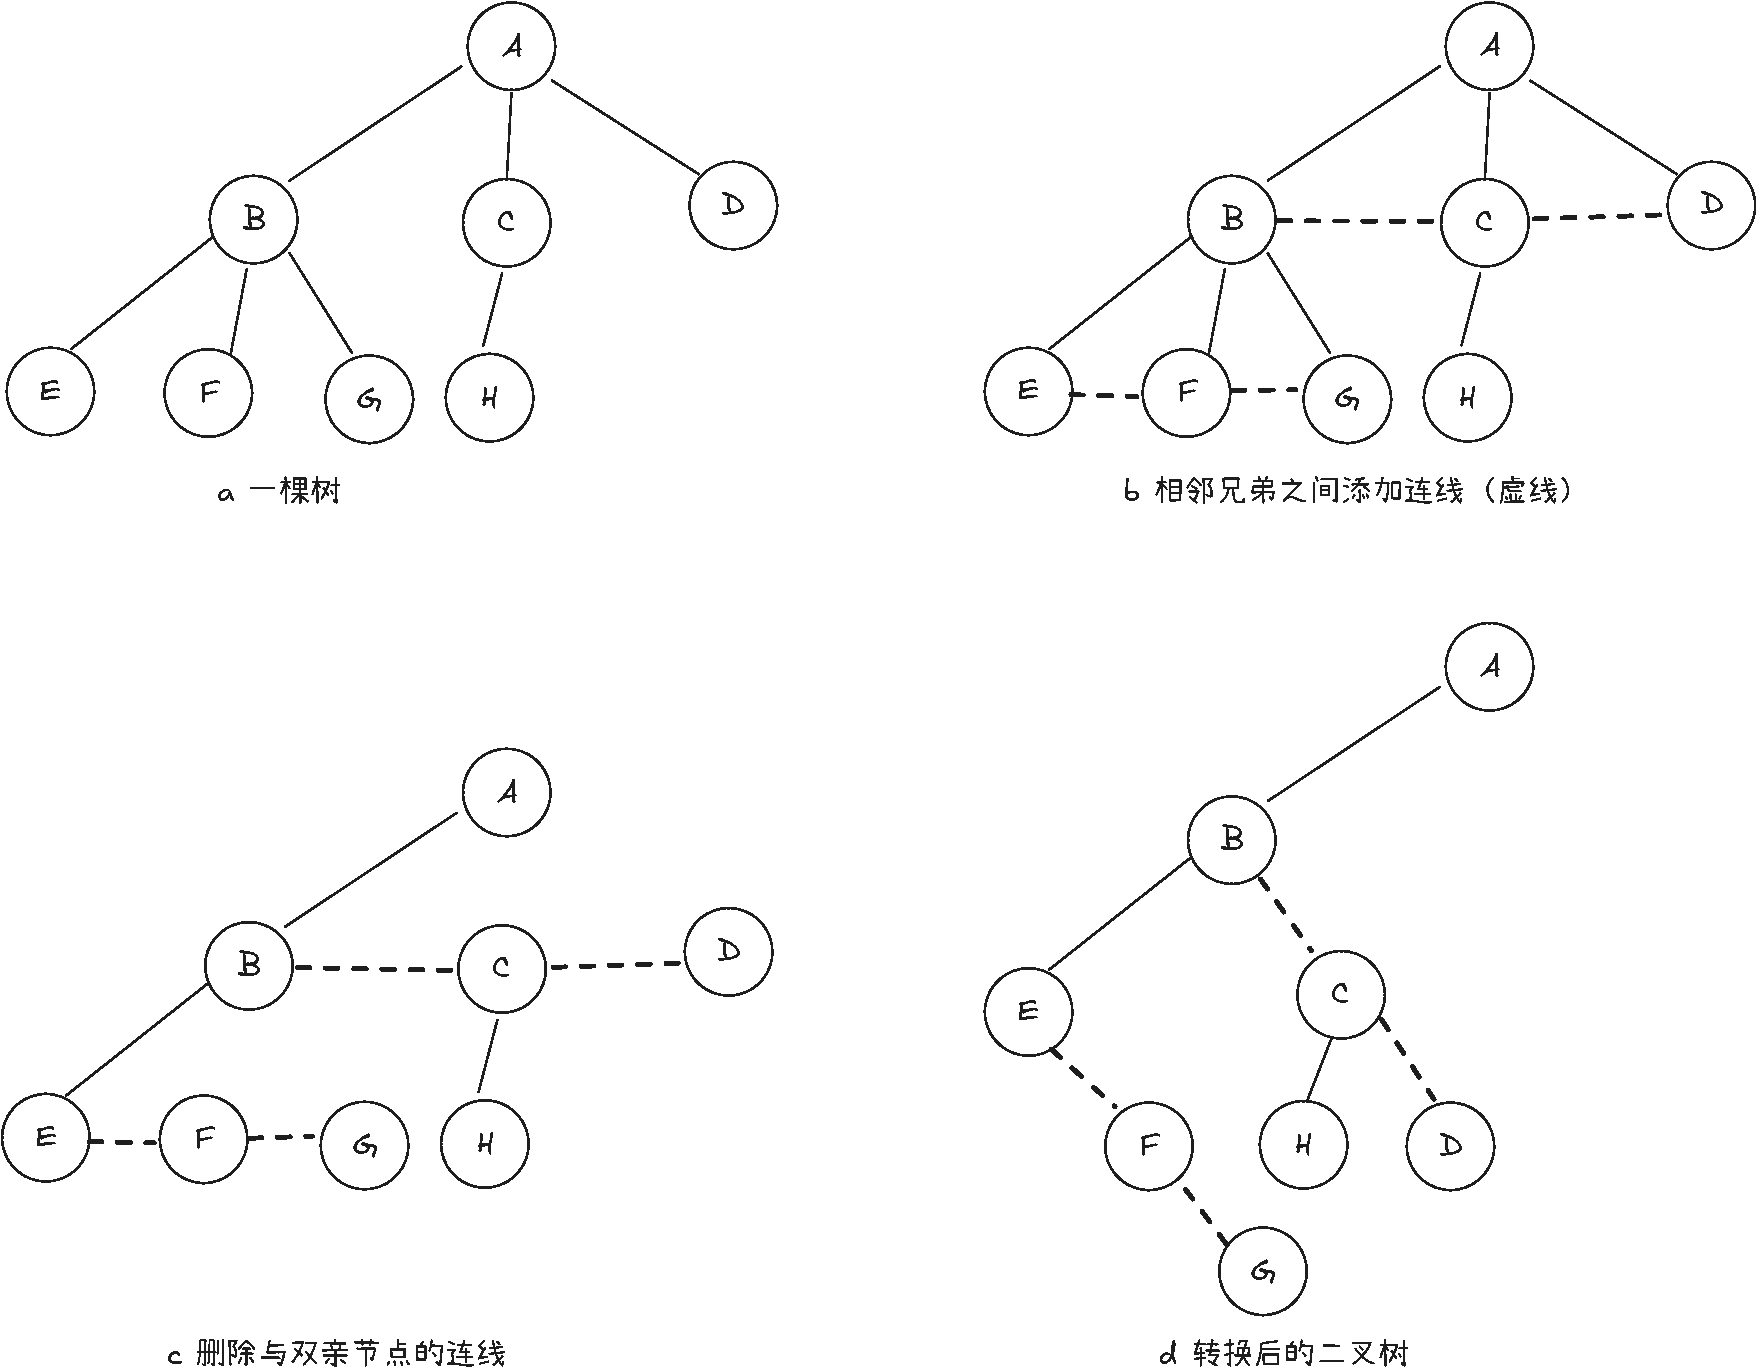
\includegraphics[width=1\textwidth]{./figure/pdf/cropped/tree2Btree.pdf}
  \caption{树转换成二叉树}
  \label{fig:tree2BiTree}
\end{figure}


若一棵二叉树是由一棵树转换而来的,则该二叉树还原为树的过程如下:

\begin{enumerate}
  \item 若某结点是其双亲的左孩子,则把该结点的右孩子、右孩子的右孩子等都与该结点的双亲结点用连线连起来;
  \item 删除原二叉树中所有双亲结点与右孩子结点之间的连线;
  \item 整理由前面两步得到的树,即以根结点为轴心,逆时针转动 $45^\circ$,使之结构层次分明。
\end{enumerate}

实际上,二叉树的还原就是将二叉树中的左分支保持不变,将二叉树中的右分支还原成兄弟关系。

如图\ref{fig:BiTree2Tree}所示,将二叉树还原成树的过程。

\begin{figure}[!htbp]
  \centering
  \includegraphics[width=1\textwidth]{./figure/pdf/cropped/Btree2Tree.pdf}
  \caption{二叉树还原成树}
  \label{fig:BiTree2Tree}
\end{figure}


\subsection{二叉树和森林的转换}

将一棵森林转换成二叉树的过程如下:
\begin{enumerate}
  \item 将森林中的每棵树转换成相应的二叉树;
  \item 第一棵二叉树不动,从第二棵二叉树开始,依次把后一棵二叉树的根结点作为前一棵二叉树根结点的右孩子结点。
  当所有二叉树连在一起后,此时得到的二叉树就是由森林转换得到的二叉树。
\end{enumerate}

实际上,当森林由两棵或两棵以上的树 $\{T_1, T_2, \dots, T_n\}$ 构成时,所有这些树的根结点构成兄弟关系。所以森林转换成一棵二叉树 $BT$ 后,
将第一棵树 $T_1$ 的根结点作为 $BT$ 的根结点,$T_2$ 的根结点作为 $T_1$ 的右孩子结点,$T_3$ 的根结点作为 $T_2$ 的右孩子结点,依此类推。

如图\ref{fig:forest2BiTree}所示,将森林转换成二叉树的过程。

\begin{figure}[!htbp]
  \centering
  \includegraphics[width=1\textwidth]{./figure/pdf/cropped/forest2Btree.pdf}
  \caption{森林转换成二叉树}
  \label{fig:forest2BiTree}
\end{figure}

将二叉树还原为森林的过程如下:

\begin{enumerate}
  \item 抹掉二叉树根结点右链上的所有结点之间的“双亲—右孩子”关系,将其分成若干个以右链上的结点为根结点的二叉树,
  设这些二叉树为 $BT_1, BT_2, \dots, BT_n$;
  \item 分别将 $BT_1, BT_2, \dots, BT_n$ 二叉树各自还原成一棵树。
\end{enumerate}

如图\ref{fig:BiTree2Forest}所示,将二叉树还原成森林的过程。

\begin{figure}[!htbp]
  \centering
  \includegraphics[width=1\textwidth]{./figure/pdf/cropped/Btree2Forest.pdf}
  \caption{二叉树还原成森林}
  \label{fig:BiTree2Forest}

\end{figure}
\section{哈夫曼树和哈夫曼编码}

\subsection{哈夫曼树}

在许多应用中,经常将树中的结点赋予一个有某种意义的数值,称此数值为该结点的权。从根结点到该结点之间的路径长度与该结点上的权的乘积称为结点的带权路径长度。树中所有叶子结点的带权路径长度之和称为树的带权路径长度,通常记为:

\[
WPL = \sum_{i=1}^{n_0} w_i l_i
\]

其中,$n_0$ 表示叶子结点的个数,$w_i$ 和 $l_i$ 分别表示第 $i$ 个叶子结点的权值和根到它之间的路径长度(即从根结点到该叶子结点的路径上经过的分支数)。

在 $n_0$ 个带权叶子结点构成的所有二叉树中,带权路径长度 $WPL$ 最小的二叉树称为哈夫曼树或最优二叉树。如图\ref{fig:weightBTree}带权二叉树,它们的带权路径长度为:

\[
\begin{cases}
(a) \ WPL = 1 \times 2 + 4 \times 3 + 5 \times 3 + 6 \times 3 = 47 \\
(b) \ WPL = 1 \times 3 + 4 \times 3 + 5 \times 2 + 6 \times 1 = 31 \\
(c) \ WPL = 1 \times 2 + 4 \times 2 + 5 \times 2 + 6 \times 2 = 32
\end{cases}
\]

\begin{figure}[!htbp]
  
  \centering

  \includegraphics[width=0.8\textwidth]{./figure/pdf/cropped/treeWeight.pdf}
  \caption{带权二叉树}
  \label{fig:weightBTree}
\end{figure}

显然,带权路径长度最小的是图\ref{fig:weightBTree}(b)的二叉树,所以图\ref{fig:weightBTree}(b)是哈夫曼树。

哈夫曼树的构造过程如下:

\begin{enumerate}
  \item 从 $n$ 个权值 $\{w_1, w_2, \dots, w_n\}$ 中选择两个最小的权值 $w_i$ 和 $w_j$,构造一棵新的二叉树,其根结点的权值为 $w_i + w_j$;
  \item 将 $w_i$ 和 $w_j$ 从权值集合中删除,将 $w_i + w_j$ 加入权值集合中;
  \item 重复上述两步,直到所有的权值都被选出,构造成一棵二叉树为止。
  \end{enumerate}

如图\ref{fig:HuffmanTree}所示,构造哈夫曼树的过程。

\begin{figure}[!htbp]
  \centering
  \includegraphics[width=1\textwidth]{./figure/pdf/cropped/createHaffman.pdf}
  \caption{构造哈夫曼树}
  \label{fig:HuffmanTree}
\end{figure}

相关定理:对于具有 $n$ 个叶子结点的哈夫曼树,其带权路径长度最小,且有 $2n-1$ 个结点,其中有 $n$ 个叶子结点,$n-1$ 个度为 $1$ 的结点。
证明:在哈夫曼树的构造过程中,每次都是将两棵树合并为一棵树,所以哈夫曼树中不存在度为 1 的结点,即 $n_1 = 0$。由二叉树的性质可知,$n_0 = n_2 + 1$,即 $n_2 = n_0 - 1$。因此:

\[
n = n_0 + n_1 + n_2 = n_0 + n_2 = n_0 + (n_0 - 1) = 2n_0 - 1
\]

其中,$n$ 表示哈夫曼树的总结点数,$n_0$ 表示叶子结点的个数,$n_1$ 表示度为 1 的结点个数,$n_2$ 表示度为 2 的结点个数。

\subsection{哈夫曼编码}
\subsubsection{哈夫曼树的结点类型定义}

我们要清楚,结点的结构体的构建都是为了更好地表述相应的构造算法,所以在这里我们要从算法的角度去分析结构体的构造。

大家可以想一想,在这里哈夫曼树应该用什么样的存储结构来表示呢?
还是和之前二叉树那样链接的方式吗?显然不恰当,因为我们会重复利用这里由两个最小权值结点之和形成的新的结点。
所以我们需要有双亲结点指向孩子结点的“指针”,而我们的哈夫曼编码是需要去判断当前结点是其双亲结点的左孩子亦或右孩子。
一般而言,左孩子编码为“0”,右孩子编码为“1”。这样的话,我们就必须有从孩子结点指向双亲的“指针”。也就是说,一般性的二叉树无法满足我们这里的要求。

因此,在这里我们设计一种新的结构体:

\begin{lstlisting}[language=C++, caption={哈夫曼树结点类型定义}]
  typedef struct HTNode {
    char data;//结点数据
    int weight;//结点权值
    int parent, lchild, rchild;//双亲、左孩子、右孩子的下标
  } HTNode, *HuffmanTree;
\end{lstlisting}

通过上述哈夫曼树的结构体,我们便可以进行哈夫曼树的构造。构造代码如下:

\begin{lstlisting}[language=C++, caption={构造哈夫曼树}]

  void Select(HuffmanTree HT, int n, int &s1, int &s2) {
    int min1 = INT_MAX, min2 = INT_MAX;
    for (int i = 1; i <= n; i++) {
      if (HT[i].parent == 0) {
        if (HT[i].weight < min1) {
          min2 = min1;
          s2 = s1;
          min1 = HT[i].weight;
          s1 = i;
        } else if (HT[i].weight < min2) {
          min2 = HT[i].weight;
          s2 = i;
        }
      }
    }
  }

  void CreateHuffmanTree(HuffmanTree &HT, int n) {
    if (n <= 1) {
      return;
    }
    int m = 2 * n - 1;
    HT = (HuffmanTree)malloc((m + 1) * sizeof(HTNode));
    if (!HT) {
      exit(OVERFLOW);
    }
    for (int i = 1; i <= m; i++) {
      HT[i].parent = 0;
      HT[i].lchild = 0;
      HT[i].rchild = 0;
    }
    for (int i = 1; i <= n; i++) {
      scanf(``%d``, &HT[i].weight);
    }
    for (int i = n + 1; i <= m; i++) {
      int s1, s2;
      Select(HT, i - 1, s1, s2);
      HT[s1].parent = i;
      HT[s2].parent = i;
      HT[i].lchild = s1;
      HT[i].rchild = s2;
      HT[i].weight = HT[s1].weight + HT[s2].weight;
    }
  }
\end{lstlisting}


进一步我们可以对哈夫曼树进行编码,代码如下:

\begin{lstlisting}[language=C++, caption={哈夫曼编码}]
  void HuffmanCoding(HuffmanTree HT, HuffmanCode &HC, int n) {
    HC = (HuffmanCode)malloc((n + 1) * sizeof(char *));
    char *cd = (char *)malloc(n * sizeof(char));
    cd[n - 1] = '\0';
    for (int i = 1; i <= n; i++) {
      int start = n - 1;
      int c = i;
      int f = HT[i].parent;
      while (f != 0) {
        --start;
        if (HT[f].lchild == c) {
          cd[start] = '0';
        } else {
          cd[start] = '1';
        }
        c = f;
        f = HT[f].parent;
      }
      HC[i] = (char *)malloc((n - start) * sizeof(char));
      strcpy(HC[i], &cd[start]);
    }
    free(cd);
  }
\end{lstlisting}

说明:在一组字符的哈夫曼编码中,各字符的编码不一定是等长的,但一定是没有前缀的。这样的编码称为前缀编码。前缀编码的一个重要性质是:任何字符的编码都不是另一个字符编码的前缀。
\section{并查集}

\textbf{并查集是什么}

所谓并查集,是用来解决元素分组问题的一种数据结构。并查集的基本操作有两个:查找和合并。查找即是找到某个元素所在的集合,合并即是将两个集合合并为一个集合。

更为形象的理解并查集:并查集的重要思想就在于要用集合中的一个元素来代表集合。就好比把集合比喻成帮派,而代表元素则是帮主。我们利用这个比喻来看看并查集是如何运作的。

初始状态如图\ref{fig:unionFind1}所示,每个元素都是一个单独的集合,每个集合的代表元素就是自己。

\begin{figure}[!htbp]
  \centering
  \includegraphics[width=0.8\textwidth]{./figure/pdf/cropped/unionFindExample(a).pdf}
  \caption{并查集初始状态}
  \label{fig:unionFind1}
\end{figure}

初始状态,所有人自成一派,自己就是帮主(对于只有一个元素的集合,代表元素自然也只能是那个唯一的元素)

现在,1号与4号进行比武,假设1号赢,那么按照江湖规矩,4号就得当1号的小弟(合并),此时1号帮派就有两个人了,帮主(代表元素就是1号)

\begin{figure}[!htbp]
  \centering
  \includegraphics[width=0.4\textwidth]{./figure/pdf/cropped/unionFindExample(b).pdf}
  \caption{并查集合并}
  \label{fig:unionFind2}
\end{figure}

过了一段时间,5号选手想和想和4号pk,首先他们得看看他们得帮主是不是同一个人,如果是同一个人那就不能开战,发现不是同一人,
5号的帮主就是他自己,而4号帮主是1号,1号出马迎接5号的挑战,假设仍然1号胜出,那么5号也必须加入1号帮派,1号仍然作为帮主。

\begin{figure}[!htbp]
  \centering
  \includegraphics[width=0.4\textwidth]{./figure/pdf/cropped/unionFindExample(c).pdf}
  \caption{并查集合并}
  \label{fig:unionFind3}
\end{figure}

假设2 3 6 号也同样进行了激烈的帮派斗争,形成以下格局:

\begin{figure}[!htbp]
  \centering
  \includegraphics[width=0.4\textwidth]{./figure/pdf/cropped/unionFindExample(d).pdf}
  \caption{并查集合并}
  \label{fig:unionFind4}
\end{figure}

现在江湖上形成了两强局面,某一天4号和6号想要pk。首先他们的帮主不是同一人,所以他们喊各自的帮主,1号和3号出手,假设1号胜利,则3号拜入1号门下,当然2号和6号作为3号小弟也成为了1号的小弟。

\begin{figure}[!htbp]
  \centering
  \includegraphics[width=0.4\textwidth]{./figure/pdf/cropped/unionFindExample(e).pdf}
  \caption{并查集合并}
  \label{fig:unionFind5}
\end{figure}

善于观察的同学已经发现这其实是一个树状的结构,要寻找集合的代表元素,只需要一步一步的向上寻找即可,可以发现,代表元素的箭头是永远指向自己的,这也是我们去判断是否找到代表元素的一个条件。

\textbf{并查集的实现}

我们上面的描述可以知道,我们的每一个结点都要能够找到他的双亲结点,而且最开始的祖先结点就是结点本身。
鉴于此我们可以设置一个数组用来达到此目的,即将数组下标代表各元素,
而下标对应的值为其双亲序号,这样层层寻找就可以找到其祖先元素。由此并查集代码实现可分为以下三个部分:

\begin{itemize}
  \item 初始化:每个元素的父亲都是自己
  \item 查找:找到元素的祖先元素
  \item 合并:将两个元素的祖先元素合并
  \end{itemize}

  初始化一个并查集:

  \begin{lstlisting}[language=C++, caption={并查集初始化}]
    void Init(int *parent, int n) {
      for (int i = 0; i < n; i++) {
        parent[i] = i;
      }
    }
  \end{lstlisting}

  查找元素的祖先元素:

  \begin{lstlisting}[language=C++, caption={查找元素的祖先元素}]
    int Find(int *parent, int i) {
      if (parent[i] == i) {
        return i;
      }
      return Find(parent, parent[i]);
    }

  \end{lstlisting}

  合并两个元素的祖先元素,即将两个“帮派”进行合并,即将前者的父节点指向后者的父节点:

  \begin{lstlisting}[language=C++, caption={合并两个元素的祖先元素}]
    void Union(int *parent, int i, int j) {
      int rootI = Find(parent, i);
      int rootJ = Find(parent, j);
      if (rootI != rootJ) {
        parent[rootI] = rootJ;
      }
    }
  \end{lstlisting}

  通过上述三个函数,我们就可以实现一个简单的并查集。并查集的应用非常广泛,比如在图的最小生成树算法中的Kruskal算法中就用到了并查集。

  \textbf{并查集的优化}

  上面的并查集的效率是比较低的,例如如果我们遇到下面的场景:

  \begin{figure}
    \centering
    \includegraphics[width=0.6\textwidth]{./figure/pdf/cropped/unionFindLow.pdf}
    \caption{并查集低效率}
    \label{fig:unionFind6}
  \end{figure}

  在合并 $2, 3$ 时,我们找到 $2$ 的祖先是 $1$,然后将 $1$ 的祖先设置为 $3$;同理,第二步时将 $3$ 的祖先设置为 $4$。大家可以发现,这样的一种做法会使得我们的查询效率变得十分低下。假如有 $10000$ 个数,那么最大的查找次数就会达到 $10000$ 次。

  而我们也可以发现,我们的目的是找到“代表元素”。直观地来看,我们完全可以将父亲节点直接设置为“代表元素”,就像这样:

  \begin{figure}[!htbp]
    \centering
    \includegraphics[width=0.6\textwidth]{./figure/pdf/cropped/pathCompress.pdf}
    \caption{并查集高效率}
    \label{fig:unionFind7}
  \end{figure}

  这样我们每次就可以以0(1)的时间复杂度找到我们的“代表元素”。这种方法也叫做路径压缩,现在我们看看代码应该如何实现,如下所示:

  \begin{lstlisting}[language=C++, caption={路径压缩}]
    int Find(int *parent, int i) {
      if (parent[i] != i) {
        parent[i] = Find(parent, parent[i]);
      }
      return parent[i];
    }

    //上述代码也可以简化为如下形式

    int Find(int *parent, int i) {
      return parent[i] == i ? i : parent[i] = Find(parent, parent[i]);
    }
  \end{lstlisting}
\chapter{图}

\section{图的基本概念}



\subsection{图的定义}
图是由两个集合,顶点集(Vertex)和边集(Edge)组成的,记为 $G = (V, E)$。其中,$V$ 是顶点的有穷非空集合,$E$ 是边的有穷集合。图中的边可以是有向的,也可以是无向的。

注:在我们的这些数据结构中,线性表可以是空表,树可以是空树,但是图不可以是空图,至少要有一个顶点。

\subsection{图的分类}

\textbf{根据图中边的有无方向,图可以分为有向图和无向图。}

\begin{itemize}
  \item 无向图:图中的边没有方向,即边 $(v_i, v_j)$ 和边 $(v_j, v_i)$ 是等价的,如图\ref{fig:undirectedGraph}所示,边 $(v_i, v_j)$ 和边 $(v_j, v_i)$ 是等价的。
  \item 有向图:图中的边有方向,即边 $(v_i, v_j)$ 和边 $(v_j, v_i)$ 是不等价的,如图\ref{fig:directedGraph}所示,边 $(v_i, v_j)$ 称为弧,$v_i$ 称为弧尾,$v_j$ 称为弧头。
  \end{itemize}

  \begin{figure}[!htbp]
    \centering
    \includegraphics[width=0.2\textwidth]{./figure/pdf/cropped/undirection.pdf}
    \caption{无向图}
    \label{fig:undirectedGraph}
  \end{figure}

  \begin{figure}[!htbp]
    \centering
    \includegraphics[width=0.2\textwidth]{./figure/pdf/cropped/direction.pdf}
    \caption{有向图}
    \label{fig:directedGraph}

  \end{figure}

  \textbf{根据图中边的权值,图可以分为无权图和带权图。}

  \begin{itemize}
    \item 无权图:图中的边没有权值,如图\ref{fig:undirectedGraph}和图\ref{fig:directedGraph}所示。
    \item 带权图:图中的边有权值,如图\ref{fig:weightedGraph}所示。
    \end{itemize}

    \begin{figure}[!htbp]
      \centering
      \includegraphics[width=0.2\textwidth]{./figure/pdf/cropped/weightedGraph.pdf}
      \caption{带权图}
      \label{fig:weightedGraph}
    \end{figure}

\textbf{简单图和多重图}

\begin{itemize}
  \item 简单图:图中不存在顶点到自身的边,且同一条边不重复出现,如图\ref{fig:simpleGraph}所示。
  \item 多重图:图中存在顶点到自身的边,或者同一条边重复出现,如图\ref{fig:multipleGraph}所示。
  \end{itemize}

  \begin{figure}[!htbp]
    \centering
    \includegraphics[width=0.2\textwidth]{./figure/pdf/cropped/unDirection.pdf}
    \caption{简单图}
    \label{fig:simpleGraph}
  \end{figure}

  \begin{figure}[!htbp]
    \centering
    \includegraphics[width=0.2\textwidth]{./figure/pdf/cropped/mutipleGraph.pdf}
    \caption{多重图}
    \label{fig:multipleGraph}
  \end{figure}

\textbf{完全图}

对于无向图,如果图中任意两个顶点之间都存在边,则称该图为完全图,如图\ref{fig:completeGraph}所示。包含 $n$ 个顶点的完全图有 $\frac{n(n-1)}{2}$ 条边。

对于有向图,如果图中任意两个顶点之间都存在方向相同的边,则称该图为完全有向图,如图\ref{fig:completeDirectedGraph}所示。包含 $n$ 个顶点的完全有向图有 $n(n-1)$ 条边。

\begin{figure}[!htbp]
  \centering
  \includegraphics[width=0.2\textwidth]{./figure/pdf/cropped/unDirection.pdf}
  \caption{完全无向图}
  \label{fig:completeGraph}

\end{figure}

\begin{figure}[!htbp]
  \centering
  \includegraphics[width=0.2\textwidth]{./figure/pdf/cropped/directedComGraph.pdf}
  \caption{完全有向图}
  \label{fig:completeDirectedGraph}
\end{figure}


\textbf{子图}

设 $G = (V, E)$ 是一个图,$G' = (V', E')$ 是 $G$ 的一个子图,如果 $V' \subseteq V$ 且 $E' \subseteq E$,则称 $G'$ 是 $G$ 的子图。如图 \ref{fig:subGraph}所示,$G'$ 是 $G$ 的子图。

\begin{figure}[!htbp]
  \centering
  \includegraphics[width=0.6\textwidth]{./figure/pdf/cropped/subGraph.pdf}
  \caption{子图}
  \label{fig:subGraph}
\end{figure}

      


\subsection{图的基本术语}


\textbf{端点和邻接点}

对于无向图,如果边 $(v_i, v_j)$ 存在,则称 $v_i$ 和 $v_j$ 互为邻接点,$v_i$ 和 $v_j$ 称为边 $(v_i, v_j)$ 的端点。

对于有向图,如果弧 $(v_i, v_j)$ 存在,则称 $v_i$ 邻接到 $v_j$,$v_i$ 称为弧 $(v_i, v_j)$ 的弧尾,$v_j$ 称为弧 $(v_i, v_j)$ 的弧头。

\textbf{度}
在无向图中,一个顶点所关联的边的数目称为该顶点的度(degree)。在有向图中,顶点的入度(indegree)是以该顶点为终点的边的数目,出度(outdegree)是以该顶点为起点的边的数目。一个顶点的入度与出度的和为该顶点的度。

若一个图中有 $n$ 个顶点和 $e$ 条边,每个顶点的度为 $d_i \ (0 \leq i \leq n-1)$,则有:

\[
e = \frac{\sum_{i=0}^{n-1} d_i}{2}
\]

也就是说,一个图中所有顶点的度之和等于边数的两倍。因为图中的每条边分别作为两个邻接点的度各计一次。

\textbf{路径和路径长度}

在图 $G = (V, E)$ 中,从顶点 $v_i$ 到顶点 $v_j$ 的路径是一个顶点序列 $v_{i_0}, v_{i_1}, \dots, v_{i_k}$,其中 $v_{i_0} = v_i$,$v_{i_k} = v_j$,且 $(v_{i_{m-1}}, v_{i_m}) \in E \ (1 \leq m \leq k)$。路径的长度是路径上边或弧的数目。

\textbf{回路或环}

如果路径的起点和终点相同,则称该路径为回路或环。

\textbf{简单路径}

如果路径中除起点和终点外,其余顶点均不相同,则称该路径为简单路径。

\textbf{连通、连通图和连通分量}

在无向图中,如果从顶点 $v_i$ 到顶点 $v_j$ 有路径,则称 $v_i$ 和 $v_j$ 是连通的。如果无向图中任意两个顶点都是连通的,则称该无向图是连通图。无向图的极大连通子图称为连通分量。

在有向图中,如果从顶点 $v_i$ 到顶点 $v_j$ 有路径,且从顶点 $v_j$ 到顶点 $v_i$ 也有路径,则称 $v_i$ 和 $v_j$ 是强连通的。如果有向图中任意两个顶点都是强连通的,则称该有向图是强连通图。有向图的极大强连通子图称为强连通分量。




\section{图的存储结构}
图的存储结构除了要存储图中各个顶点本身的信息以外,同时还要存储顶点与顶点之
间的所有关系(边的信息)。常用的图的存储结构有邻接矩阵和邻接表。 本他主要这论首
两种存储结构和基本运算算法的设计。

\subsection{邻接矩阵}
图的邻接矩阵是一种采用邻接矩阵数组表示顶点之间相邻关系的存储结构。
邻接矩阵说白了就是一个二维数组,数组下标代表顶点序号,数组值,即行列交叉处代表两个顶点之间的权值,如果是无权图,
那么我们简单设置为1即可。如果两顶点之间没有边,
那我们就可以将数组对应位置设置为$\infty$ 或者0都可以。

不带权无向图的邻接矩阵如图\ref{fig:adjacencyMatrix_UnWeightUndirected}所示。

\begin{figure}[!htbp]
  \centering
  \includegraphics[width=0.8\textwidth]{./figure/pdf/cropped/adjacencyMatrix_UnWeightUndirected.pdf}
  \caption{无权无向图的邻接矩阵}
  \label{fig:adjacencyMatrix_UnWeightUndirected}
\end{figure}

带权有向图的邻接矩阵如图\ref{fig:adjacencyMatrix_WeightedDirected}所示。

\begin{figure}[!htbp]
  \centering
  \includegraphics[width=0.8\textwidth]{./figure/pdf/cropped/adjacencyMatrix_weightDirected.pdf}
  \caption{带权有向图的邻接矩阵}
  \label{fig:adjacencyMatrix_WeightedDirected}
\end{figure}


带权无向图的邻接矩阵如图\ref{fig:adjacencyMatrix_WeightedUndirected}所示。
\begin{figure}[!htbp]
  \centering
  \includegraphics[width=0.8\textwidth]{./figure/pdf/cropped/adjacencyMatrix_weightUnDirected.pdf}
  \caption{邻接矩阵}
  \label{fig:adjacencyMatrix_WeightedUndirected}
\end{figure}

由此可见,邻接矩阵的结构体可以定义如下:

\begin{lstlisting}[language=C++, caption={邻接矩阵结构体}]
  #define MAX_VERTEX_NUM 20
  typedef struct {
    char vexs[MAX_VERTEX_NUM];//顶点表
    int arc[MAX_VERTEX_NUM][MAX_VERTEX_NUM];//邻接矩阵
    int vexnum, arcnum;//顶点数和边数
  } MGraph;
\end{lstlisting}

\textbf{邻接矩阵的特点}

\begin{itemize}
  \item 图的邻接矩阵表示唯一,无向图的邻接矩阵是对称的。
  \item 对于含有 $n$ 个顶点的图,当采用邻接矩阵表示时,需要 $n^2$ 个存储单元,因此,邻接矩阵的存储空间是 $O(n^2)$。所以邻接矩阵适合存储边数相对较多的图。
  \item 对于无向图,邻接矩阵中的非零元素的个数是边的条数的两倍。
  \item 对于有向图,邻接矩阵中的非零元素的个数是边的条数。
  \item 对于无向图,邻接矩阵数组的第 $i$ 行或第 $i$ 列中非零元素的个数是顶点 $v_i$ 的度。
  \item 对于有向图,邻接矩阵数组的第 $i$ 行中非零元素的个数是顶点 $v_i$ 的出度,第 $i$ 列中非零元素的个数是顶点 $v_i$ 的入度。
  \item 在邻接矩阵中,判断图中两个顶点之间是否有边或者边的权值是非常方便的,只需要 $O(1)$ 的时间。
  \end{itemize}


\subsection{邻接表}
图的邻接表是一种采用链式存储结构表示顶点之间相邻关系的存储结构。邻接表是图的一种链式存储结构,
它的基本思想是:对图 $G$ 的每个顶点 $v_i$,建立一个单链表,
链表中的结点称为顶点 $v_i$ 的边表,边表中的结点存储了与顶点 $v_i$ 相邻接的顶点在顶点表中的位置和边上的权值。如图 \ref{fig:adjacencyList} 所示。

\begin{figure}[!htbp]
  \centering
  \includegraphics[width=0.8\textwidth]{./figure/pdf/cropped/adjacencyList.pdf}
  \caption{邻接表}
  \label{fig:adjacencyList}
\end{figure}

对邻接表的理解:

首先我们要明白结构体是可以嵌套的,也就是说结构体中可以有结构体,这样我们就可以很方便地表示图的结构。第一步划分如图\ref{fig:adjacencyList_struct}所示,
我们可以看到,整个邻接表被我们划分为三个单链表,其实也很容易想到,我们说过邻接表是顺序表和链表的结合,
当我们单独划分出单链表的时候,那么第一个节点就是我们的头结点,比如上面的0号位置的结点1,1号位置的结点2..,
然后我们可以发现,我有很多个头结点,每一个头结点都引出了该节点的邻接顶点,那同样地,我们很自然地想到用一个数组来存储我们的头结点,
即我们构造一个顶点数组,数组中的元素类型为顶点,包含顶点本身信息,和指向下一个邻接点的指针,显然的是,
图中的每一个顶点均会作为头结点来连接它的邻接顶点,哪怕没有邻接点(如点3)。

\begin{figure}[!htbp]
  \centering
  \includegraphics[width=0.6\textwidth]{./figure/pdf/cropped/adjacencyList_struct.pdf}
  \caption{邻接表结构体}
  \label{fig:adjacencyList_struct}
\end{figure}

接下来我们进一步拆分,以1号顶点为例,如图 \ref{fig:adjacencyList_struct2}所示,我们可以看到,绿色框框出的就是单个链表所基于的最小单位,
也就是我们所说的单表结点,注意这里头结点和后续结点不是完全一样的,
头结点属于顶点表数组,其结点为顶点表节点,而后续结点则是表达邻接点的关系,属于边表结点。

其中,顶点表结点包含顶点信息info和第一条邻接边firstEdge;
边表结点包含该顶点在顶点表数组中的下标(这样我们就可以很容易拿到该顶点的信息以及连接信息)、到该邻接点的边的权重以及下一个邻接点(同样是边表结点)。
经过上面的阐释我们的顶点表结点的结构体以及边表结点结构体也就呼之欲出了。如代码所示:

\begin{figure}[!htbp]
  \centering
  \includegraphics[width=0.6\textwidth]{./figure/pdf/cropped/adjacencyList_struct2.pdf}
  \caption{邻接表结构体}
  \label{fig:adjacencyList_struct2}

\end{figure}

\begin{lstlisting}[language=C++, caption={邻接表结构体}]
  typedef struct EdgeNode {
    int adjvex;//邻接点域
    int weight;//权值
    struct EdgeNode *next;//指针域
  } EdgeNode;

  typedef struct VertexNode {
    char data;//顶点域
    EdgeNode *firstEdge;//边表头指针
  } VertexNode;

\end{lstlisting}

但这里我们可以发现,如果仅使用上面两个结构体,我们可能只能表示一个顶点的邻接关系,还记得我们说过,
全部的顶点都归属于同一个顶点表数组吗,在这里我们就需要创建一个顶点表数组,将所有的顶点都放入这个数组,通过数组来访问其顶点信息以及邻接点信息。如代码所示:

\begin{lstlisting}[language=C++, caption={邻接表结构体}]
  #define MAX_VERTEX_NUM 20
  typedef struct {
    VertexNode adjList[MAX_VERTEX_NUM];//顶点表
    int numVertexes, numEdges;//顶点数和边数
  } ALGraph;
\end{lstlisting}

可以看到,我们在ALGraph中创建了一个顶点数组,数组元素类型为VertexNode,即顶点表类型,然后还设立了边数和顶点数,这两个信息是基础信息,会时常用到。
如图 \ref{fig:adjacencyList_struct3}所示。

\begin{figure}[!htbp]
  \centering
  \includegraphics[width=0.6\textwidth]{./figure/pdf/cropped/adjList_array.pdf}
  \caption{邻接表结构体}
  \label{fig:adjacencyList_struct3}
\end{figure}

邻接表的特点如下:

\begin{enumerate}
  \item 邻接表的表示不唯一,这是因为在每个顶点对应的单链表中,各边结点的链接次序可以是任意的,取决于建立邻接表的算法以及边的输入次序。
  
  \item 对于有 $n$ 个顶点和 $e$ 条边的无向图,其邻接表有 $n$ 个头结点和 $2e$ 个边结点;对于有 $n$ 个顶点和 $e$ 条边的有向图,其邻接表有 $n$ 个头结点和 $e$ 个边结点。显然,对于边数目较少的稀疏图,邻接表比邻接矩阵更节省存储空间。
  
  \item 对于无向图,邻接表中顶点 $v_i$ 对应的第 $i$ 个单链表的边结点数目正好是顶点 $v_i$ 的度。
  
  \item 对于有向图,邻接表中顶点 $v_i$ 对应的第 $i$ 个单链表的边结点数目仅仅是顶点 $v_i$ 的出度。顶点 $v_j$ 的入度为邻接表中所有 $adjvex$ 域值为 $v_j$ 的边结点数目。
  
  \item 在邻接表中,查找顶点 $v_i$ 关联的所有边是非常快速的,所以在需要提取某个顶点的所有邻接点的算法中通常采用邻接表存储结构。
\end{enumerate}
\subsection{十字链表}

\subsection{邻接多重表}

\section{图的基本运算}


\subsection{图的创建}

\subsubsection{邻接矩阵的创建}

我们可以根据用户的输入来创建一个图的邻接矩阵,首先输入顶点数和边数,然后输入顶点信息,最后输入边的信息,即边的两个顶点的下标和权值。

\begin{lstlisting}[language=C++, caption={邻接矩阵的创建}]
  void CreateMGraph(MGraph *G) {
    int i, j, k, w;
    printf(``输入顶点数和边数:\n``);
    scanf(``%d %d``, &G->vexnum, &G->arcnum);
    printf(``输入顶点信息:\n``);
    for (i = 0; i < G->vexnum; i++) {
      scanf(``%c``, &G->vexs[i]);
    }
    for (i = 0; i < G->vexnum; i++) {
      for (j = 0; j < G->vexnum; j++) {
        G->arc[i][j] = 0;
      }
    }
    for (k = 0; k < G->arcnum; k++) {
      printf(``输入边(vi, vj)的下标i, 下标j和权值w:\n``);
      scanf(``%d %d %d``, &i, &j, &w);
      G->arc[i][j] = w;
      G->arc[j][i] = w;
    }
  }
\end{lstlisting}

\subsubsection{邻接表的创建}

我们可以根据用户的输入来创建一个图的邻接表,首先输入顶点数和边数,然后输入顶点信息,最后输入边的信息,即边的两个顶点的下标。
\begin{lstlisting}[language=C++, caption={邻接表的创建}]
  void CreateALGraph(ALGraph *G) {
    int i, j, k;
    EdgeNode *e;
    printf(``输入顶点数和边数:\n``);
    scanf(``%d %d``, &G->numVertexes, &G->numEdges);
    printf(``输入顶点信息:\n``);
    for (i = 0; i < G->numVertexes; i++) {
      scanf(``%c``, &G->adjList[i].data);
      G->adjList[i].firstEdge = NULL;
    }
    for (k = 0; k < G->numEdges; k++) {
      printf(``输入边(vi, vj)的下标i, 下标j:\n``);
      scanf(``%d %d``, &i, &j);
      e = (EdgeNode *)malloc(sizeof(EdgeNode));
      e->adjvex = j;
      e->next = G->adjList[i].firstEdge;
      G->adjList[i].firstEdge = e;

      e = (EdgeNode *)malloc(sizeof(EdgeNode));
      e->adjvex = i;
      e->next = G->adjList[j].firstEdge;
      G->adjList[j].firstEdge = e;
    }
  }

\end{lstlisting}

\subsection{输出图}

\subsubsection{邻接矩阵的输出}

\begin{lstlisting}[language=C++, caption={邻接矩阵的输出}]
  void PrintMGraph(MGraph G) {
    int i, j;
    for (i = 0; i < G.vexnum; i++) {
      for (j = 0; j < G.vexnum; j++) {
        printf(``%d ``, G.arc[i][j]);
      }
      printf(``\n``);
    }
  }
\end{lstlisting}

\subsubsection{邻接表的输出}

扫描邻接表G的头结点数组adjlist,对于每个单链表,先输出头结点的信息,然后扫描边表,输出边表结点的信息。
\begin{lstlisting}[language=C++, caption={邻接表的输出}]
  void PrintALGraph(ALGraph G) {
    int i;
    EdgeNode *e;
    for (i = 0; i < G.numVertexes; i++) {
      printf(``%c``, G.adjList[i].data);
      e = G.adjList[i].firstEdge;
      while (e != NULL) {
        printf(``%d``, e->adjvex);
        e = e->next;
      }
      printf(``\n``);
    }
  }
\end{lstlisting}


\section{图的遍历}
从给定图中任意指定的顶点(称为初始点)出发,按照某种搜索方法沿着图的边访问图中的所有顶点,使每个顶点仅被访问一次,这个过程称为图的遍历。
如果给定图是连通的无向图或者是强连通的有向图,则遍历过程一次就能完成,并可按访问的先后顺序得到由该图的所有顶点组成的一个序列。

图的遍历比树的遍历更复杂,因为从树根到达树中的任意结点只有一条路径,而从图的初始点到达图中的每个顶点可能存在着多条路径。
当沿着图中的一条路径访问过某一顶点之后,可能还沿着另一条路径回到该顶点,即存在回路。为了避免同一个顶点被重复访问,必须记住每个被访问过的顶点。
为此,可设置一个访问标记数组 \texttt{visited},当顶点 $v_i$ 被访问过时,数组中的元素 \texttt{visited[$i$]} 置为 $1$,否则置为 $0$。

根据搜索方法的不同,图的遍历方法有两种:
\begin{itemize}
  \item 深度优先遍历(Depth First Search, DFS);
  \item 广度优先遍历(Breadth First Search, BFS)。
\end{itemize}
\subsection{深度优先搜索}

\subsubsection{深度优先搜索的基本思想}
深度优先遍历见名知意,就是在图的遍历中,从初始顶点开始,不断地往更深处去遍历。假设我们从图中的某个初始点 $i$ 出发,首先访问该初始点,
然后选择一个与顶点 $i$ 相邻且未被访问过的顶点 $j$,再以 $j$ 为初始顶点,从它出发进行深度优先遍历,直到图中所有的顶点全部被访问完。

从以上描述可以看出,深度优先遍历其实是一个递归过程。

如图 \ref{fig:DFS} 所示,从顶点 $v_0$ 出发,首先访问顶点 $1$,然后选择与顶点 $1$ 相邻且未被访问过的顶点 $1$,再以 $1$ 为初始顶点,
从它出发进行深度优先遍历,直到图中所有的顶点全部被访问完。那么访问序列为:1 2 3 4或1 2 4 3。

注意:深度优先遍历可能会产生不同的遍历序列,主要是因为我们去选择邻接点时可能存在多个邻接点 ,这就使得深优序列可能不同*

\begin{figure}[!htbp]
  \centering
  \includegraphics[width=0.2\textwidth]{./figure/pdf/cropped/depthFirstGraph.pdf}
  \caption{深度优先搜索}
  \label{fig:DFS}
\end{figure}

其深度优先访问过程如图 \ref{fig:depthFirst} 所示。可以大致分为以下几步:

\begin{itemize}
  \item 初始顶点为 $1$,访问顶点 $1$,将 \texttt{visited} 数组对应位置置为 $1$,然后寻找邻接点 $2$。  
  \item 判断顶点 $2$ 未被访问,递归调用深度优先算法,以 $2$ 为“起始点”,访问顶点 $2$,将 \texttt{visited} 数组对应位置置为 $1$,然后寻找邻接点 $4$。  
  \item 判断顶点 $4$ 未被访问,递归调用深度优先算法,以 $4$ 为“起始点”,访问顶点 $4$,将 \texttt{visited} 数组对应位置置为 $1$,然后寻找邻接点。  
  \item 未找到邻接点,退出以顶点 $4$ 为“起始点”的递归,回到以 $2$ 为“起始点”的递归,继续寻找邻接点 $3$。  
  \item 判断顶点 $3$ 未被访问,递归调用深度优先算法,以 $3$ 为“起始点”,访问顶点 $3$,将 \texttt{visited} 数组对应位置置为 $1$,然后寻找邻接点 $2$。  
  \item 判断邻接点 $2$ 已被访问,不再进入递归。  
  \item 顶点 $3$ 无其他未被访问的邻接点,退出以顶点 $3$ 为“起始点”的递归,回到以 $2$ 为“起始点”的递归,继续寻找邻接点。  
  \item 顶点 $2$ 无其他未被访问的邻接点,退出以顶点 $2$ 为“起始点”的递归,回到以 $1$ 为“起始点”的递归,继续寻找邻接点。  
  \item 顶点 $1$ 无其他未被访问的邻接点,退出以顶点 $1$ 为“起始点”的递归,程序结束。
\end{itemize}

\begin{figure}[!htbp]
  \centering
  \includegraphics[width=0.6\textwidth]{./figure/pdf/cropped/depthFirst.pdf}
  \caption{深度优先搜索}
  \label{fig:depthFirst}
\end{figure}


\subsubsection{深度优先搜索的实现}
紧接着我们将上述过程转化为代码,如下所示:

\textbf{邻接表DFS}

\begin{lstlisting}[language=C++, caption={邻接表DFS}]
  void DFS(ALGraph G, int i) {
    EdgeNode *p;
    visited[i] = 1;
    printf(``%c``, G.adjList[i].data);
    p = G.adjList[i].firstEdge;
    while (p != NULL) {
      if (!visited[p->adjvex]) {
        DFS(G, p->adjvex);
      }
      p = p->next;
    }
  }
\end{lstlisting}

空间复杂度 $O(n)$,这是因为 $visited$ 数组的大小为 $n$,递归调用的深度最大为 $n$。

时间复杂度为 $O(n+e)$,其中 $n$ 为顶点数,$e$ 为边数。因为每个顶点只会被访问一次,每条边也只会被访问一次。

\textbf{邻接矩阵DFS}

\begin{lstlisting}[language=C++, caption={邻接矩阵DFS}]
  void DFS(MGraph G, int i) {
    int j;
    visited[i] = 1;
    printf(``%c``, G.vexs[i]);
    for (j = 0; j < G.vexnum; j++) {
      if (G.arc[i][j] == 1 && !visited[j]) {
        DFS(G, j);
      }
    }
  }
\end{lstlisting}

\textbf{空间复杂度}:由于 DFS 是一个递归算法,递归需要一个工作栈来辅助工作,最多需要图中所有顶点进栈,所以空间复杂度为 $O(|V|)$。

\textbf{时间复杂度}:
\begin{itemize}
  \item \textbf{邻接表}:遍历过程的主要操作是对顶点遍历它的邻接点,由于通过访问边表来查找邻接点,所以时间复杂度为 $O(|E|)$;访问顶点的时间为 $O(|V|)$,所以总的时间复杂度为 $O(|V| + |E|)$。
  \item \textbf{邻接矩阵}:查找每个顶点的邻接点时间复杂度为 $O(|V|)$,对每个顶点都进行查找,所以总的时间复杂度为 $O(|V|^2)$。
\end{itemize}


\subsection{广度优先搜索}

\subsubsection{广度优先搜索的基本思想}

广度优先搜索是一种从图中某个顶点 $v$ 出发,首先访问顶点 $v$,然后依次访问 $v$ 的各个未曾访问过的邻接点,再依次访问这些邻接点的邻接点,直到图中所有顶点都被访问过为止。

广度优先搜索的访问过程如图 \ref{fig:breadthFirst} 所示,我们从顶点1开始,最终遍历序列为 1 2 3 4 5 6或1 3 2 4 5 6。

注意:广度优先遍历可能会产生不同的遍历序列,主要是因为我们去选择邻接点时可能存在多个邻接点 ,这就使得广度优序列可能不同。

\begin{figure}[!htbp]
  \centering
  \includegraphics[width=1\textwidth]{./figure/pdf/cropped/breadthFirst.pdf}
  \caption{广度优先搜索}
  \label{fig:breadthFirst}
\end{figure}


\subsubsection{广度优先搜索的实现}

\textbf{邻接表BFS}

\begin{lstlisting}[language=C++, caption={邻接表BFS}]
  void BFS(ALGraph G, int i) {
    int j;
    EdgeNode *p;
    int queue[MAX_VERTEX_NUM];
    int front = 0, rear = 0;
    printf(``%c``, G.adjList[i].data);
    visited[i] = 1;
    rear = (rear + 1) % MAX_VERTEX_NUM;
    queue[rear] = i;
    while (front != rear) {
      front = (front + 1) % MAX_VERTEX_NUM;
      j = queue[front];
      p = G.adjList[j].firstEdge;
      while (p != NULL) {
        if (!visited[p->adjvex]) {
          printf(``%c``, G.adjList[p->adjvex].data);
          visited[p->adjvex] = 1;
          rear = (rear + 1) % MAX_VERTEX_NUM;
          queue[rear] = p->adjvex;
        }
        p = p->next;
      }
    }
  }

\end{lstlisting}

\textbf{邻接矩阵BFS}

\begin{lstlisting}[language=C++, caption={邻接矩阵BFS}]
  void BFS(MGraph G, int i) {
    int j;
    int queue[MAX_VERTEX_NUM];
    int front = 0, rear = 0;
    printf(``%c``, G.vexs[i]);
    visited[i] = 1;
    rear = (rear + 1) % MAX_VERTEX_NUM;
    queue[rear] = i;
    while (front != rear) {
      front = (front + 1) % MAX_VERTEX_NUM;
      j = queue[front];
      for (int k = 0; k < G.vexnum; k++) {
        if (G.arc[j][k] == 1 && !visited[k]) {
          printf(``%c``, G.vexs[k]);
          visited[k] = 1;
          rear = (rear + 1) % MAX_VERTEX_NUM;
          queue[rear] = k;
        }
      }
    }
  }
\end{lstlisting}

\textbf{空间复杂度}:由于 BFS 是一个迭代算法,需要一个队列来辅助工作,最多需要图中所有顶点进队列,所以空间复杂度为 $O(|V|)$。

\textbf{时间复杂度}:

\begin{itemize}
  \item \textbf{邻接表}:遍历过程的主要操作是对顶点遍历它的邻接点,由于通过访问边表来查找邻接点,所以时间复杂度为 $O(|E|)$;访问顶点的时间为 $O(|V|)$,所以总的时间复杂度为 $O(|V| + |E|)$。
  \item \textbf{邻接矩阵}:查找每个顶点的邻接点时间复杂度为 $O(|V|)$,对每个顶点都进行查找,所以总的时间复杂度为 $O(|V|^2)$。
  \end{itemize}

\section{最小生成树}
一个连通图的生成树(spanning tree)是一个极小连通子图,其中含有图中的全部顶点,和构成一棵树的 $(n-1)$ 条边。如果在一棵生成树上添加任何一条边,必定构成一个环,因为添加的这条边使得它关联的那两个顶点之间有了第 2 条路径。

一棵有 $n$ 个顶点的生成树(连通无回路图)有且仅有 $(n-1)$ 条边。如果一个图有 $n$ 个顶点和小于 $(n-1)$ 条边,则是非连通图。如果它多于 $(n-1)$ 条边,则一定有回路。

对于一个带权(假设每条边上的权均为大于零的实数)连通无向图 $G$ 中的不同生成树,其每棵树的所有边上的权值之和也可能不同;图的所有生成树中具有边上的权值之和最小的树称为图的最小生成树(minimal spanning tree)。

按照生成树的定义,$n$ 个顶点的连通图的生成树有 $n$ 个顶点和 $(n-1)$ 条边。因此,构造最小生成树的准则有以下 3 条:

\begin{enumerate}
  \item 必须只使用该图中的边来构造最小生成树;
  \item 必须使用且仅使用 $(n-1)$ 条边来连接图中的所有顶点;
  \item 不能使用产生回路的边。
\end{enumerate}

求图的最小生成树有很多实际应用,例如城市之间的交通工程造价最优问题就是一个最小生成树问题。
求图的最小生成树的两个算法即普里姆算法(Prim 算法)和克鲁斯卡尔算法(Kruskal 算法),将在后面介绍。
\subsection{Prim算法}
普利姆(Prim)算法是一种构造性算法。假设 $G = (V, E)$ 是一个具有 $n$ 个顶点的带权连通图,$T = (U, TE)$ 是 $G$ 的最小生成树,其中 $U$ 是 $T$ 的顶点集,$TE$ 是 $T$ 的边集,则由 $G$ 构造从起点 $v$ 出发的最小生成树 $T$ 的步骤如下:

\begin{itemize}
  \item ① 从图中找第一个起始顶点 $v_0$,作为生成树的第一个顶点,然后从这个顶点到其他顶点的所有边中选一条权值最小的边。然后把这条边的另一个顶点 $v$ 和这条边加入到生成树中。
  \item ② 对剩下的其他所有顶点,分别检查这些顶点与顶点 $v$ 的权值是否比这些顶点在 \texttt{lowcost} 数组中对应的权值小,如果更小,则用较小的权值更新 \texttt{lowcost} 数组。
  \item ③ 从更新后的 \texttt{lowcost} 数组中继续挑选权值最小而且不在生成树中的边,然后加入到生成树。
  \item ④ 反复执行步骤 ② 和 ③,直到所有顶点都加入到生成树中。
\end{itemize}

如图\ref{fig:prim}所示,我们形象地观察其构造过程:



\begin{figure}[!htbp]
  \centering
  \includegraphics[width=1\textwidth]{./figure/pdf/cropped/prime.pdf}
  \caption{Prim算法}
  \label{fig:prim}
\end{figure}

从上面的例子可以看出,Prim 算法是一种增量算法,逐步选择最小边,并在 $U$ 集合中添加相应的顶点。每一步都是从 $U$ 和 $V-U$ 两个顶点集合中选择最小边,并在前面的基础上进行扩展。现在我们来分析如何使用代码实现 Prim 算法:

\begin{itemize}
  \item 首先,我们尝试在邻接矩阵的基础上实现 Prim 算法。因为 Prim 算法会频繁地取一条条边的权值,所以采用邻接矩阵更合适。当然,后面我们也会用邻接表的方式实现。
  
  \item 当我们拿到一个连通图的邻接矩阵时,我们需要从给定顶点开始,依次加入当前最小边。对于 Prim 函数而言,首先需要传入图和起点。

  \item 回想一下我们是如何选出第一条边的:首先将起点 $0$ 到其他顶点的直接距离记录下来。我们会发现 $0$ 只能到达 $1$ 和 $5$,其余全是无穷。然后根据规则,选择最小的距离对应的顶点,即顶点 $5$。为了实现这一逻辑,我们可以用一个数组存储 $0$ 号顶点到其他顶点的距离,并将其命名为 \texttt{lowCost}。初始状态为:
  \[
  \texttt{lowCost} = [0, 28, 32767, 32767, 32767, 10, 32767]
  \]
  其中,$32767$ 表示无穷大。

  \item 当我们有了 \texttt{lowCost} 数组后,就可以选出 $5$ 号顶点。接下来,我们需要更新 \texttt{lowCost} 数组。根据 Prim 算法,每次从新加入集合的顶点出发,寻找当前可达的最短距离顶点。例如,在加入 $5$ 号顶点后,之前 $0$ 号顶点无法到达的顶点现在通过 $5$ 号顶点可以到达了,比如 $4$ 号顶点。此时,\texttt{lowCost} 更新为:
  \[
  \texttt{lowCost} = [0, 28, 32767, 32767, 25, 10, 32767]
  \]

  \item 为了避免重复选择已经加入集合的顶点,我们可以使用一个标志数组 \texttt{visited}。初始状态为:
  \[
  \texttt{visited} = [0, 0, 0, 0, 0, 0, 0]
  \]
  当加入 $0$ 号顶点时,更新为:
  \[
  \texttt{visited} = [1, 0, 0, 0, 0, 0, 0]
  \]
  当加入 $5$ 号顶点时,更新为:
  \[
  \texttt{visited} = [1, 0, 0, 0, 1, 0, 0]
  \]

  \item 当所有顶点都加入后,整个寻找过程结束。为了存储寻找结果,可以用一个二维数组存储每次加入的边,或者用一个一维数组存储每次加入的顶点,以便复盘时快速还原最小生成树。
\end{itemize}

至此,Prim 算法的关键逻辑已经清晰。接下来,我们通过实际的 C 语言代码实现 Prim 算法:

\begin{lstlisting}[language=C++, caption={Prim算法}]
  void prim(AMGraph* G, int start) {
	int flag[MAXSIZE];//标记数组
	int lowCost[MAXSIZE];//当前已加入最小生成树的邻接顶点的边的权值
	int prims[MAXSIZE];//存储最小生成树结果数组
	int record,index=0;
	for (int i = 0; i < G->numV; i++) {
		lowCost[i] = G->Edge[start][i];//初始化start到各顶点的距离
		prims[i] = 0;//初始化
		flag[i] = 0;
	}
	flag[start] = 1;//传入的顶点设为已访问
	prims[index++] = start;
	for (int i = 1; i < G->numV; i++) {//因为源点已加入集合,则共进行G->numV-1次循环
		int min = 32767;
		//找目前能到达的权值最小顶点
		for (int j = 0; j < G->numV; j++) {
			if (!flag[j] && lowCost[j] < min) {//lowCost不为0代表未访问过
				min = lowCost[j];
				record = j;
			}
		}
		flag[record] = 1;
		prims[index++] = record;//一旦发生更换将m处的值设为record,代表由record处的顶点指向m处的顶点目前最近,即record是m的前驱
		//当我们加入新顶点时,我们要判断加入新顶点后是否路径会缩短,如果有这种情况,就要更新lowCost
		for (int m = 0; m < G->numV; m++) {
			if (!flag[m] && lowCost[m] > G->Edge[record][m]) {//当前 记录的从源点到record的距离 大于 加入record后的距离,进行更新!!
				lowCost[m] = G->Edge[record][m] ;
			}
		}
	}
	printf(``%d ``, getSum(G, prims));
	for (int i = 0; i < G->numV; i++) {
		printf(``%c ``, G->Vertex[prims[i]]);
	}
}

以上代码是在邻接矩阵存储方式中进行prim算法的写法,而在邻接表中进行操作,整体算法思想并无不同,
但是因为存储方式的不同,会在有些地方进行对应调整,代码如下,有兴趣的同学可以细细研究:

void prim(ALGraph* G, int start) {
  /*
	prim算法(采用邻接表):
		算法核心:
				根据邻接矩阵改编!!
*/
#include <stdio.h>
#include <stdlib.h>
#include ``ALGraphStruct.h``//通过头文件加载邻接表结构体
int getSum(ALGraph* G, int* lowCost) {//获得最小生成树的权值
	int sum = 0;
	for (int i = 0; i < G->numV; i++) {
		sum += lowCost[i];
	}
	return sum;
}
void primInAL(ALGraph *G, int start) {
	int prims[MAXSIZE];//存储最小生成树结果数组
	int lowCost[MAXSIZE];//当前已加入最小生成树的邻接顶点的权值
	int flag[MAXSIZE];
	int min, index, primIndex = 0;// min 寻找最小值  index 记录最小值下标 primIndex prim数组下标 
	for (int i = 0; i < G->numV; i++) {
		lowCost[i] = 32767;//把所有值设为无穷
		flag[i] = 0;
		prims[i] = -1;
	}
	//初始化
	for (EdgeNode *p = G->adjlist[start].firstEdge; p; p = p->next) {
		lowCost[p->index] = p->weight;//把当前传入顶点的所有连接顶点的边的权值存入
	}
	lowCost[start] = 0;//自己到自己的距离为0
	prims[primIndex++] = start;//将源点加入生成树数组
	flag[start] = 1;
	for (int i = 0; i < G->numV-1; i++) {//进行顶点数-1轮的循环,每次循环加入一个顶点
		min = 32767;
		for (int j = 0; j < G->numV; j++) {
			if (!flag[j] && lowCost[j] < min) {//如果当前顶点未曾加入最小树中且小于目前最小值,更新
				min = lowCost[j];
				index = j;//记录位置
			}

		}
		//已找到最小值,更新prims数组
		prims[primIndex++] = index;
		//lowCost[index] = 0;//将第index个顶点置为已访问,即代表它已加入最小生成树
		flag[index] = 1;
		//如有顶点未处理,则看情况需更新lowCost数组
		EdgeNode* p = G->adjlist[index].firstEdge;//寻找下标为index的顶点可到达的顶点
		while (p) {
			if (!flag[p->index] && p->weight < lowCost[p->index]) {//在index处的旧值大于我们加入新节点后的
				lowCost[p->index] = p->weight;
			}
			p = p->next;
		}
		
	}
	printf(``最小生成树权值为:%d ``, getSum(G, lowCost));
	printf(``\n``);
	for (int i = 0; i < G->numV; i++) {
		printf(``%c ``, G->adjlist[prims[i]].info);
	}

}

int main() {
	ALGraph *G = (ALGraph *)malloc(sizeof(ALGraph));
	void createGraphFromFile(ALGraph *);
	void dispGraph(ALGraph *);
	createGraphFromFile(G);//创建图
	dispGraph(G);
	primInAL(G, 0);
	return 0;
}
\end{lstlisting}
\subsection{Kruskal算法}
Kruskal 算法是基于贪心思想得到的。首先,我们将所有的边按照权值从小到大排序,接着按照顺序选取每条边。如果这条边的两个端点不属于同一集合,那么就将它们合并,直到所有的点都属于同一个集合为止。至于如何合并到一个集合,这里我们可以用到一个工具——并查集(Union-Find)。换而言之,Kruskal 算法就是基于并查集的贪心算法。

我们用下面的流程图来模拟 Kruskal 算法的过程,并简单描述其步骤:

\begin{itemize}
  \item 首先,Kruskal 算法是一个不断添加边的操作方法。我们会从未选择的边中选取当前权值最小的边加入集合,且不构成环。显然,边 $\langle 0, 5 \rangle$ 符合条件。
  \item 然后选择边 $\langle 2, 3 \rangle$、$\langle 1, 6 \rangle$ 和 $\langle 1, 2 \rangle$。
  \item 此时剩下的边有 5 条,最小的是边 $\langle 3, 6 \rangle$,权值为 18。但是我们不能选择这一条边,因为如果选择它,就会产生环,这是不允许的。所以我们只能退而求其次选择边 $\langle 3, 4 \rangle$,权值为 22。
  \item 最后,同样的道理,按理说权值最小的边是 $\langle 4, 6 \rangle$,但是如果加入这条边就会形成环,所以我们选择边 $\langle 4, 5 \rangle$。
  \item 到这里,我们已经加入了 $n-1$ 条边($n$ 是顶点数),已经找到最小生成树,算法结束。
\end{itemize}

\begin{figure}[!htbp]
  \centering
  \includegraphics[width=1\textwidth]{./figure/pdf/cropped/kruskal.pdf}
  \caption{Kruskal算法}
  \label{fig:kruskal}
\end{figure}
代码分析构造:

\begin{itemize}
  \item 整个 Kruskal 算法并不复杂,我们用邻接矩阵存储来进行分析。Kruskal 的整体思路无非就是不断加入当前最小的边并确保不构成环。
  
  \item 首先我们可以确定的是,与 Prim 算法不同,这一次并不需要指定起点,我们只需要传入整幅图即可。
  
  \item 在这里,我们直接给出避免形成环的方法——并查集。在后续章节中我们会详细讲解,这里大家先有一个概念即可,记住并查集可以帮助我们避免形成环。
  
  \item 接下来就是常规的代码逻辑了,指定一个循环,该循环保证我们能够加入 $n-1$ 条边。
  
  \item 然后找到符合不形成环的最小权值边,加入最小生成树集合。
\end{itemize}

\begin{lstlisting}[language=C++, caption={Kruskal算法}]
  /*
	kruskal 算法:每次选择最短的一条边加入集合,直至所有顶点被包含,而且会用到并查集
*/
#include<stdio.h>
#include <stdlib.h>
#include ``ALGraphStruct.h``//通过头文件加载邻接表结构体

void outPut(ALGraph *G, int **weights) {//输出最小生成树
	for (int i = 0; i < G->numV; i++) {
		for (int j = i; j < G->numV; j++) {
			if (weights[i][j] != 0) {
				printf(``%c->%c(%d)\n``, G->adjlist[i].info, G->adjlist[j].info, weights[i][j]);
			}
		}
	}
}
int findAncestor(int *fa, int i) {
	if (fa[i] == i)return i;//找到返回
	else {
		fa[i] = findAncestor(fa, i);//路径压缩
		return findAncestor(fa,fa[i]);
	}
}
void unionn(int *fa, int i, int j) {
	int i_a = findAncestor(fa, i);
	int j_a = findAncestor(fa, j);
	fa[i_a] = j_a;//i的祖先指向j的祖先
}
void kruskal(ALGraph *G) {
	int **weights = (int **)malloc(sizeof(int *)*G->numV);//两点间的权值数据
	int *fa = (int *)malloc(sizeof(int)*G->numV);//并查集数组
	for (int i = 0; i < G->numV; i++) {
		fa[i] = i;//最开始将每个节点的祖先设置为自己
	}
	for (int i = 0; i < G->numV; i++) {
		weights[i] = (int *)malloc(sizeof(int)*G->numV);
	}
	for (int i = 0; i < G->numV; i++) {
		for (int j = 0; j < G->numV; j++) {
			weights[i][j] = 0;//初始化该二位数组
		}
	}
	int edges = 0;
	while (edges < G->numV - 1) {//最小生成树的边数一定是顶点数减一
		int weight = 32767;
		int start, end;
		for (int i = 0; i < G->numV; i++) {//遍历每一个顶点的所有边
			for (EdgeNode *p = G->adjlist[i].firstEdge; p; p = p->next) {
				//寻找最短边
				if (p->weight < weight && findAncestor(fa, i) != findAncestor(fa, p->index)) {
					weight = p->weight;
					start = i;
					end = p->index;
				}
			}
		}
		unionn(fa, start, end);
		weights[start][end] = weight;
		weights[end][start] = weight;
		edges++;
	}
	outPut(G, weights);

}
int main() {
	ALGraph *G = (ALGraph *)malloc(sizeof(ALGraph));
	void createGraphFromFile(ALGraph *);
	void dispGraph(ALGraph *);
	createGraphFromFile(G);//创建图
	dispGraph(G);
	kruskal(G);
	return 0;
}

\end{lstlisting}
\section{最短路径}
在一个不带权图中,若从一个顶点到另一个顶点存在着一条路径,则称该路径长度为该路径上所经过的边的数目,它等于该路径上的顶点数减 $1$。由于从一顶点到另一顶点可能存在着多条路径,每条路径上所经过的边数可能不同,即路径长度不同,把路径长度最短(即经过的边数最少)的那条路径称为最短路径,其长度称为最短路径长度或最短距离。

对于带权图,考虑路径上各边上的权,则把一条路径上所经过的权之和定义为该路径的路径长度。从源点到终点可能有不止一条路径,把路径长度最小的那条路径称为最短路径,其路径长度(权之和)称为最短路径长度。

实际上,只要把不带权图上的每条边看成是权值为 $1$ 的边,那么不带权图和带权图的最短路径和最短距离的定义就一致了。

求图的最短路径有两个方面的问题:
\begin{itemize}
  \item 求图中某一顶点到其余各顶点的最短路径;
  \item 求图中每一对顶点之间的最短路径。
\end{itemize}
\subsection{Dijkstra算法}
迪杰斯特拉(Dijkstra)算法不太容易理解,我们先从一个例子着手:

\begin{figure}[!htbp]
  \centering
  \includegraphics[width=0.6\textwidth]{./figure/pdf/cropped/directedWeightGraph.pdf}
  \caption{一个带权有向图}
  \label{fig:dijkstra}
\end{figure}

\textbf{Dijkstra算法的执行过程:}

\begin{enumerate}
  \item \textbf{初始化}:  
  $S = \{0\}, U = \{1, 2, 3, 4, 5, 6\}$,  
  $\texttt{dist} = [0, 4, 6, 6, \infty, \infty, \infty]$(源点 $0$ 到其他各顶点的权值,直接来源于邻接矩阵),  
  $\texttt{path} = [0, 0, 0, 0, -1, -1, -1]$(若源点 $0$ 到顶点 $i$ 有边 $\langle 0, i \rangle$,则 $\texttt{path}[i] = 0$;否则 $\texttt{path}[i] = -1$ 表示没有路径)。

  \item 从 $U$ 中找最小的顶点(即 $\texttt{dist}$ 值最小的顶点)为顶点 $1$,将它添加到 $S$ 中:  
  $S = \{0, 1\}, U = \{2, 3, 4, 5, 6\}$。  
  考查顶点 $1$,发现从顶点 $1$ 到顶点 $2$ 和 $4$ 有边:
  \[
  \texttt{dist}[2] = \min(\texttt{dist}[2], \texttt{dist}[1] + 1) = 5 \quad (\text{修改})
  \]
  \[
  \texttt{dist}[4] = \min(\texttt{dist}[4], \texttt{dist}[1] + 7) = 11 \quad (\text{修改})
  \]
  更新后:  
  $\texttt{dist} = [0, 4, 5, 6, 11, \infty, \infty]$,  
  $\texttt{path} = [0, 0, 1, 0, 1, -1, -1]$。

  \item 从 $U$ 中找最小的顶点为顶点 $2$,将它添加到 $S$ 中:  
  $S = \{0, 1, 2\}, U = \{3, 4, 5, 6\}$。  
  考查顶点 $2$,发现从顶点 $2$ 到顶点 $4$ 和 $5$ 有边:
  \[
  \texttt{dist}[4] = \min(\texttt{dist}[4], \texttt{dist}[2] + 6) = 11
  \]
  \[
  \texttt{dist}[5] = \min(\texttt{dist}[5], \texttt{dist}[2] + 4) = 9 \quad (\text{修改})
  \]
  更新后:  
  $\texttt{dist} = [0, 4, 5, 6, 11, 9, \infty]$,  
  $\texttt{path} = [0, 0, 1, 0, 1, 2, -1]$。

  \item 从 $U$ 中找最小的顶点为顶点 $3$,将它添加到 $S$ 中:  
  $S = \{0, 1, 2, 3\}, U = \{4, 5, 6\}$。  
  考查顶点 $3$,发现从顶点 $3$ 到顶点 $2$ 和 $5$ 有边,但顶点 $2$ 已经考查过,不进行修改:
  \[
  \texttt{dist}[5] = \min(\texttt{dist}[5], \texttt{dist}[3] + 5) = 9
  \]
  无修改,$\texttt{dist}$ 和 $\texttt{path}$ 不变。

  \item 从 $U$ 中找最小的顶点为顶点 $5$,将它添加到 $S$ 中:  
  $S = \{0, 1, 2, 3, 5\}, U = \{4, 6\}$。  
  考查顶点 $5$,发现从顶点 $5$ 到顶点 $4$ 和 $6$ 有边:
  \[
  \texttt{dist}[4] = \min(\texttt{dist}[4], \texttt{dist}[5] + 1) = 10 \quad (\text{修改})
  \]
  \[
  \texttt{dist}[6] = \min(\texttt{dist}[6], \texttt{dist}[5] + 8) = 17 \quad (\text{修改})
  \]
  更新后:  
  $\texttt{dist} = [0, 4, 5, 6, 10, 9, 17]$,  
  $\texttt{path} = [0, 0, 1, 0, 5, 2, 5]$。

  \item 从 $U$ 中找最小的顶点为顶点 $4$,将它添加到 $S$ 中:  
  $S = \{0, 1, 2, 3, 5, 4\}, U = \{6\}$。  
  考查顶点 $4$,发现从顶点 $4$ 到顶点 $6$ 有边:
  \[
  \texttt{dist}[6] = \min(\texttt{dist}[6], \texttt{dist}[4] + 6) = 16 \quad (\text{修改})
  \]
  更新后:  
  $\texttt{dist} = [0, 4, 5, 6, 10, 9, 16]$,  
  $\texttt{path} = [0, 0, 1, 0, 5, 2, 4]$。

  \item 从 $U$ 中找最小的顶点为顶点 $6$,将它添加到 $S$ 中:  
  $S = \{0, 1, 2, 3, 5, 4, 6\}, U = \{\}$。  
  从顶点 $6$ 不能到达任何顶点,过程结束。其过程如下表所示。

  \item \textbf{输出最短路径}:  
  以源点 $0$ 到顶点 $6$ 的最短路径为例,$\texttt{dist}[6] = 16$,即最短路径长度为 $16$。  
  $\texttt{path}[6] = 4, \texttt{path}[4] = 5, \texttt{path}[5] = 2, \texttt{path}[2] = 1, \texttt{path}[1] = 0$,  
  反推出最短路径为 $0 \to 1 \to 2 \to 5 \to 4 \to 6$。
\end{enumerate}
从源点 $0$ 到所有其他顶点的最短路径结果如下:

\begin{itemize}
  \item 从顶点 $0$ 到顶点 $1$ 的路径长度为:$4$,路径为:$0 \to 1$。
  \item 从顶点 $0$ 到顶点 $2$ 的路径长度为:$5$,路径为:$0 \to 1 \to 2$。
  \item 从顶点 $0$ 到顶点 $3$ 的路径长度为:$6$,路径为:$0 \to 3$。
  \item 从顶点 $0$ 到顶点 $4$ 的路径长度为:$10$,路径为:$0 \to 1 \to 2 \to 5 \to 4$。
  \item 从顶点 $0$ 到顶点 $5$ 的路径长度为:$9$,路径为:$0 \to 1 \to 2 \to 5$。
  \item 从顶点 $0$ 到顶点 $6$ 的路径长度为:$16$,路径为:$0 \to 1 \to 2 \to 5 \to 4 \to 6$。
\end{itemize}
\textbf{Dijkstra算法的特点:}

\begin{itemize}
  \item (1) 在执行中,一个顶点一旦添加到 $S$ 中后,其最短路径长度不再改变。
  \item (2) 正是由于具有特点 (1),所以 Dijkstra 算法不适合含有负权值的带权图求单源最短路径。
  通过一个反例说明:假设一个含有 3 个顶点的带权有向图,$\langle 0, 1 \rangle$ 的权值为 $1$,$\langle 0, 2 \rangle$ 的权值
  为 $2$,$\langle 2, 1 \rangle$ 的权值为 $-3$,如图 \ref{fig:negativeWeight} 所示。
  若源点为 $0$,在执行 Dijkstra 算法时,首先选取的中间点为 $1$,求出源点 $0$ 到顶点 $1$ 的最短路径长度为 $1$,以后不再改变。
  而实际上,$0 \to 2 \to 1$ 才是源点 $0$ 到顶点 $1$ 的最短路径,其长度为 $-1$。
  
  \item (3) 按顶点进入 $S$ 的先后顺序,最短路径长度越来越长。
\end{itemize}

\begin{figure}[!htbp]
  \centering
  \includegraphics[width=0.2\textwidth]{./figure/pdf/cropped/negativeWeightGraph.pdf}
  \caption{含有负权值的带权图}
  \label{fig:negativeWeight}
\end{figure}

\textbf{初始化}
\[
S = \{0\}, \quad U = \{1, 2, 3, 4, 5, 6\}
\]

\[
\text{dist} =
\begin{array}{c|ccccccc}
 & 0 & 1 & 2 & 3 & 4 & 5 & 6 \\ \hline
\text{dist} & 0 & 4 & 6 & 6 & \infty & \infty & \infty 
\end{array}
\]

\[
\text{path} =
\begin{array}{c|ccccccc}
 & 0 & 1 & 2 & 3 & 4 & 5 & 6 \\ \hline
\text{path} & 0 & 0 & 0 & 0 & -1 & -1 & -1
\end{array}
\]

\textbf{步骤 1:选择最短路径的顶点 1}
\[
S = \{0,1\}, \quad U = \{2, 3, 4, 5, 6\}
\]

\[
\text{dist} =
\begin{array}{c|ccccccc}
 & 0 & 1 & 2 & 3 & 4 & 5 & 6 \\ \hline
\text{dist} & 0 & 4 & 5 & 6 & 11 & \infty & \infty 
\end{array}
\]

\[
\text{path} =
\begin{array}{c|ccccccc}
 & 0 & 1 & 2 & 3 & 4 & 5 & 6 \\ \hline
\text{path} & 0 & 0 & 1 & 0 & 1 & -1 & -1
\end{array}
\]

\textbf{步骤 2:选择最短路径的顶点 2}
\[
S = \{0,1,2\}, \quad U = \{3, 4, 5, 6\}
\]

\[
\text{dist} =
\begin{array}{c|ccccccc}
 & 0 & 1 & 2 & 3 & 4 & 5 & 6 \\ \hline
\text{dist} & 0 & 4 & 5 & 6 & 11 & 9 & \infty
\end{array}
\]

\[
\text{path} =
\begin{array}{c|ccccccc}
 & 0 & 1 & 2 & 3 & 4 & 5 & 6 \\ \hline
\text{path} & 0 & 0 & 1 & 0 & 1 & 2 & -1
\end{array}
\]

\textbf{步骤 3:选择最短路径的顶点 3}
\[
S = \{0,1,2,3\}, \quad U = \{4, 5, 6\}
\]

\[
\text{dist} =
\begin{array}{c|ccccccc}
 & 0 & 1 & 2 & 3 & 4 & 5 & 6 \\ \hline
\text{dist} & 0 & 4 & 5 & 6 & 11 & 9 & \infty
\end{array}
\]

\[
\text{path} =
\begin{array}{c|ccccccc}
 & 0 & 1 & 2 & 3 & 4 & 5 & 6 \\ \hline
\text{path} & 0 & 0 & 1 & 0 & 1 & 2 & -1
\end{array}
\]

\textbf{步骤 4:选择最短路径的顶点 5}
\[
S = \{0,1,2,3,5\}, \quad U = \{4, 6\}
\]

\[
\text{dist} =
\begin{array}{c|ccccccc}
 & 0 & 1 & 2 & 3 & 4 & 5 & 6 \\ \hline
\text{dist} & 0 & 4 & 5 & 6 & 10 & 9 & 17
\end{array}
\]

\[
\text{path} =
\begin{array}{c|ccccccc}
 & 0 & 1 & 2 & 3 & 4 & 5 & 6 \\ \hline
\text{path} & 0 & 0 & 1 & 0 & 5 & 2 & 5
\end{array}
\]

\textbf{步骤 5:选择最短路径的顶点 4}
\[
S = \{0,1,2,3,5,4\}, \quad U = \{6\}
\]

\[
\text{dist} =
\begin{array}{c|ccccccc}
 & 0 & 1 & 2 & 3 & 4 & 5 & 6 \\ \hline
\text{dist} & 0 & 4 & 5 & 6 & 10 & 9 & 16
\end{array}
\]

\[
\text{path} =
\begin{array}{c|ccccccc}
 & 0 & 1 & 2 & 3 & 4 & 5 & 6 \\ \hline
\text{path} & 0 & 0 & 1 & 0 & 5 & 2 & 4
\end{array}
\]

\textbf{步骤 6:选择最短路径的顶点 6}
\[
S = \{0,1,2,3,5,4,6\}, \quad U = \emptyset
\]

\[
\text{dist} =
\begin{array}{c|ccccccc}
 & 0 & 1 & 2 & 3 & 4 & 5 & 6 \\ \hline
\text{dist} & 0 & 4 & 5 & 6 & 10 & 9 & 16
\end{array}
\]

\[
\text{path} =
\begin{array}{c|ccccccc}
 & 0 & 1 & 2 & 3 & 4 & 5 & 6 \\ \hline
\text{path} & 0 & 0 & 1 & 0 & 5 & 2 & 4
\end{array}
\]

对应的 Dijkstra 算法如下($v$为源点):

\begin{lstlisting}[language=C++, caption={Dijkstra算法}]
  /*
  迪杰斯特拉算法:求单源最短路径
*/
#include<stdio.h>
#include <stdlib.h>
#include ``ALGraphStruct.h``//通过头文件加载邻接表结构体
void dijkstra(ALGraph *G, int v) {
  int *dist = (int *)malloc(sizeof(int)*G->numV);//源点到各点的最短路径长度
  int *path = (int *)malloc(sizeof(int)*G->numV);//源点到各点的最短路径
  int *flag = (int *)malloc(sizeof(int)*G->numV);//标记是否已经加入最短路径
  for (int i = 0; i < G->numV; i++) {
    dist[i] = G->Edge[v][i];
    flag[i] = 0;
    if (G->Edge[v][i] < 32767) {
      path[i] = v;
    }
    else {
      path[i] = -1;
    }
  }
  dist[v] = 0;
  flag[v] = 1;
  for (int i = 0; i < G->numV; i++) {
    int min = 32767;
    int u = v;
    for (int j = 0; j < G->numV; j++) {
      if (!flag[j] && dist[j] < min) {
        u = j;
        min = dist[j];
      }
    }
    flag[u] = 1;
    for (int j = 0; j < G->numV; j++) {
      if (!flag[j] && G->Edge[u][j] < 32767) {
        if (dist[j] > dist[u] + G->Edge[u][j]) {
          dist[j] = dist[u] + G->Edge[u][j];
          path[j] = u;
        }
      }
    }
  }
  for (int i = 0; i < G->numV; i++) {
    printf(``源点到%d的最短路径长度为:%d\n``, i, dist[i]);
  }
  for (int i = 0; i < G->numV; i++) {
    printf(``源点到%d的最短路径为:``, i);
    int j = i;
    while (j != v) {
      printf(``%d<-``, j);
      j = path[j];
    }
    printf(``%d\n``, v);
  }
}
int main() {
  ALGraph *G = (ALGraph *)malloc(sizeof(ALGraph));
  void createGraphFromFile(ALGraph *);
  void dispGraph(ALGraph *);
  createGraphFromFile(G);//创建图
  dispGraph(G);
  dijkstra(G, 0);
  return 0;
}
\end{lstlisting}


\subsection{Floyd算法}

Floyd 算法是一种动态规划算法,用于求解带权图中各对顶点之间的最短路径。
Floyd 算法的基本思想是:假设图 $G$ 中的顶点集合为 $\{0, 1, 2, \ldots, n-1\}$,对于任意两个顶点
 $i$ 和 $j$,我们定义 $k$ 为从 $0$ 到 $n-1$ 中的一个数,如果顶点 $k$ 在顶点 $i$ 到顶点 $j$ 的路径上,
 则顶点 $k$ 是从顶点 $i$ 到顶点 $j$ 的中间顶点。Floyd 算法的基本思想是:对于每一对顶点 $i$ 和 $j$,
 我们检查是否存在顶点 $k$ 使得从顶点 $i$ 到顶点 $k$ 再到顶点 $j$ 的路径比已知的从顶点 $i$ 到顶点 $j$ 的路径更短。
 如果是,我们更新从顶点 $i$ 到顶点 $j$ 的路径为更短的路径。我们以下图为例进行说明。

\begin{figure}[!htbp]
  \centering
  \includegraphics[width=0.4\textwidth]{./figure/pdf/cropped/floyd_directedWeightGraph.pdf}
  \caption{一个带权有向图}
  \label{fig:floyd}
\end{figure}

\textbf{Floyd算法的执行过程:}
 



\textbf{初始邻接矩阵}
给定图的初始邻接矩阵为:
\[
D^{(-1)} =
\begin{bmatrix}
0 & 5 & \infty & 7 \\
\infty & 0 & 4 & 2 \\
3 & 3 & 0 & 2 \\
\infty & \infty & 1 & 0
\end{bmatrix}
\]

初始路径矩阵为:
\[
P^{(-1)} =
\begin{bmatrix}
-1 & 0 & -1 & 0 \\
-1 & -1 & 1 & 1 \\
2 & 2 & -1 & 2 \\
-1 & -1 & 3 & -1
\end{bmatrix}
\]


\textbf{1. 以顶点 0 作为中间点}

通过顶点 0 作为中间点计算最短路径矩阵:
\[
D^{(0)} =
\begin{bmatrix}
0 & 5 & \infty & 7 \\
\infty & 0 & 4 & 2 \\
3 & 3 & 0 & 2 \\
\infty & \infty & 1 & 0
\end{bmatrix}
\]
矩阵无变化。

路径矩阵 \( P^{(0)} \) 也保持不变:
\[
P^{(0)} =
\begin{bmatrix}
-1 & 0 & -1 & 0 \\
-1 & -1 & 1 & 1 \\
2 & 2 & -1 & 2 \\
-1 & -1 & 3 & -1
\end{bmatrix}
\]

\textbf{2. 以顶点 1 作为中间点}

通过顶点 1 作为中间点计算最短路径矩阵:
\[
D^{(1)} =
\begin{bmatrix}
0 & 5 & 9 & 7 \\
\infty & 0 & 4 & 2 \\
3 & 3 & 0 & 2 \\
\infty & \infty & 1 & 0
\end{bmatrix}
\]
更新:
\[
D[0][2] = 9, \quad P[0][2] = 1
\]

更新后的路径矩阵 \( P^{(1)} \) 为:
\[
P^{(1)} =
\begin{bmatrix}
-1 & 0 & 1 & 0 \\
-1 & -1 & 1 & 1 \\
2 & 2 & -1 & 2 \\
-1 & -1 & 3 & -1
\end{bmatrix}
\]

\textbf{3. 以顶点 2 作为中间点}

通过顶点 2 作为中间点计算最短路径矩阵:
\[
D^{(2)} =
\begin{bmatrix}
0 & 5 & 9 & 7 \\
7 & 0 & 4 & 2 \\
3 & 3 & 0 & 2 \\
4 & 4 & 1 & 0
\end{bmatrix}
\]
更新:
\[
D[3][1] = 4, \quad P[3][1] = 2
\]

更新后的路径矩阵 \( P^{(2)} \) 为:
\[
P^{(2)} =
\begin{bmatrix}
-1 & 0 & 1 & 0 \\
2 & -1 & 1 & 1 \\
2 & 2 & -1 & 2 \\
2 & 2 & 3 & -1
\end{bmatrix}
\]

\textbf{4. 以顶点 3 作为中间点}

通过顶点 3 作为中间点计算最短路径矩阵:
\[
D^{(3)} =
\begin{bmatrix}
0 & 5 & 8 & 7 \\
6 & 0 & 3 & 2 \\
3 & 3 & 0 & 2 \\
4 & 4 & 1 & 0
\end{bmatrix}
\]
更新:
\[
D[0][2] = 8, \quad D[1][0] = 6, \quad D[1][2] = 3
\]

更新后的路径矩阵 \( P^{(3)} \) 为:
\[
P^{(3)} =
\begin{bmatrix}
-1 & 0 & 3 & 0 \\
2 & -1 & 3 & 1 \\
2 & 2 & -1 & 2 \\
2 & 2 & 3 & -1
\end{bmatrix}
\]

\textbf{最终最短路径矩阵}

最终计算得到的最短路径矩阵为:
\[
D =
\begin{bmatrix}
0 & 5 & 8 & 7 \\
6 & 0 & 3 & 2 \\
3 & 3 & 0 & 2 \\
4 & 4 & 1 & 0
\end{bmatrix}
\]

\textbf{最终路径矩阵}

最终计算得到的路径矩阵为:
\[
P =
\begin{bmatrix}
-1 & 0 & 3 & 0 \\
2 & -1 & 3 & 1 \\
2 & 2 & -1 & 2 \\
2 & 2 & 3 & -1
\end{bmatrix}
\]

在考试中,如果我们对于每一个顶点都要去进行计算,那么计算量十分巨大,所以我们在考试中可以通过一些小技巧来作出不同顶点加入后的最短路径矩阵。

具体规则就是:

\begin{itemize}
  \item 对角线永远为0;
  \item 以哪个顶点为中间点,就在该点为中心画出十字线,十字线上的数据不变;
  \item 如果十字线上有$\infty$ ,那么$\infty$ 对应的横线或者竖线上的数据同样不变;
  \item 其余数据则需要进行比较,如果横线上的数据大于十字线上的数据加上竖线上的数据,那么横线上的数据就变为十字线上的数据加上竖线上的数据。
\end{itemize}


上述规则应用与图 \ref{fig:floyd} 中的图,其过程如下图所示。

\textbf{第一步,加入顶点 0}:

\begin{figure}[!htbp]
  \centering
  \includegraphics[width=0.8\textwidth]{./figure/pdf/cropped/floyd_addNum0.pdf}
  \caption{加入顶点 0}
  \label{fig:floyd_0}
\end{figure}

\textbf{第二步,加入顶点 1}:

\begin{figure}[!htbp]
  \centering
  \includegraphics[width=0.8\textwidth]{./figure/pdf/cropped/floyd_addNum1.pdf}
  \caption{加入顶点 1}
  \label{fig:floyd_1}

\end{figure}

\textbf{第三步,加入顶点 2}:

\begin{figure}[!htbp]
  \centering
  \includegraphics[width=0.8\textwidth]{./figure/pdf/cropped/floyd_addNum2.pdf}
  \caption{加入顶点 2}
  \label{fig:floyd_2}

\end{figure}

\textbf{第四步,加入顶点 3}:

\begin{figure}[!htbp]
  \centering
  \includegraphics[width=0.8\textwidth]{./figure/pdf/cropped/floyd_addNum3.pdf}
  \caption{加入顶点 3}
  \label{fig:floyd_3}

\end{figure}


上述过程对应的 Floyd 算法如下:

\begin{lstlisting}[language=C++, caption={Floyd算法}]
  /*
  Floyd算法:求多源最短路径
*/
#include<stdio.h>
#include <stdlib.h>
#include ``ALGraphStruct.h``//通过头文件加载邻接表结构体
void floyd(ALGraph *G) {
  int **dist = (int **)malloc(sizeof(int *)*G->numV);//源点到各点的最短路径长度
  int **path = (int **)malloc(sizeof(int *)*G->numV);//源点到各点的最短路径
  for (int i = 0; i < G->numV; i++) {
    dist[i] = (int *)malloc(sizeof(int)*G->numV);
    path[i] = (int *)malloc(sizeof(int)*G->numV);
    for (int j = 0; j < G->numV; j++) {
      dist[i][j] = G->Edge[i][j];
      if (G->Edge[i][j] < 32767) {
        path[i][j] = i;
      }
      else {
        path[i][j] = -1;
      }
    }
  }
  for (int k = 0; k < G->numV; k++) {
    for (int i = 0; i < G->numV; i++) {
      for (int j = 0; j < G->numV; j++) {
        if (dist[i][j] > dist[i][k] + dist[k][j]) {
          dist[i][j] = dist[i][k] + dist[k][j];
          path[i][j] = path[k][j];
        }
      }
    }
  }
  for (int i = 0; i < G->numV; i++) {
    for (int j = 0; j < G->numV; j++) {
      printf(``源点%d到%d的最短路径长度为:%d\n``, i, j, dist[i][j]);
    }
  }
  for (int i = 0; i < G->numV; i++) {
    for (int j = 0; j < G->numV; j++) {
      printf(``源点%d到%d的最短路径为:``, i, j);
      int k = j;
      while (k != i) {
        printf(``%d<-``, k);
        k = path[i][k];
      }
      printf(``%d\n``, i);
    }
  }
}
int main() {
  ALGraph *G = (ALGraph *)malloc(sizeof(ALGraph));
  void createGraphFromFile(ALGraph *);
  void dispGraph(ALGraph *);
  createGraphFromFile(G);//创建图
  dispGraph(G);
  floyd(G);
  return 0;
}
\end{lstlisting}

输出多源最短路径的display()函数如下:

\begin{lstlisting}[language=C, caption={输出最短路径的 Dispath 函数}]
  void Dispath(MatGraph g, int A[MAXV][MAXV], int path[MAXV][MAXV]) {
      int i, j, k, s;
      int apath[MAXV], d; // 存放一条最短路径中间顶点(反向)及其顶点个数
  
      for (i = 0; i < g.n; i++) {
          for (j = 0; j < g.n; j++) {
              if (A[i][j] != INF && i != j) { // 若顶点 i 和 j 之间存在路径
                  printf(``从顶点 %d 到顶点 %d 的路径为: ``, i, j);
                  k = path[i][j];
                  d = 0;
                  apath[d] = j; // 路径上添加终点
                  while (k != -1 && k != i) { // 路径上添加中间点
                      d++;
                      apath[d] = k;
                      k = path[i][k];
                  }
                  d++;
                  apath[d] = i; // 路径上添加起点
                  printf(``%d``, apath[d]); // 输出起点
                  for (s = d - 1; s >= 0; s--) { // 输出路径上的中间顶点
                      printf(``, %d``, apath[s]);
                  }
                  printf(``\t路径长度为: %d\n``, A[i][j]);
              }
          }
      }
  }
  \end{lstlisting}

\section{拓扑排序}

设 $G = (V, E)$ 是一个具有 $n$ 个顶点的有向图,$V$ 中的顶点序列 $w_1, w_2, \dots, w_n$ 称为一个拓扑序列(topological sequence)。若 $\langle w_i, w_j \rangle$ 是图中的一条边或者从顶点 $w_i$ 到顶点 $w_j$ 有路径,则在该序列中顶点 $w_i$ 必须排在顶点 $w_j$ 之前。

在一个有向图中找一个拓扑序列的过程称为拓扑排序(topological sort)。

例如,计算机专业的学生必须完成一系列规定的基础课和专业课才能毕业,假设这些课程的名称与相应代号如表 \ref{tab:course} 所示:

\begin{table}[!htbp]
  \centering
  \caption{课程名称与相应代号的关系}
  \label{tab:course}
  \begin{tabular}{|c|c|c|}
    \hline
    课程代号 & 课程名称 & 先修课程 \\ \hline
    G & 高等数学 & 无 \\ \hline
    C & 程序设计 & 无 \\ \hline
    D & 离散数学 & G \\ \hline
    E & 数据结构 & C \\ \hline
    F & 编译原理 & E \\ \hline
    H & 操作系统 & E \\ \hline
    I & 计算机组成原理 & H \\ \hline
  \end{tabular}
\end{table}

课程之间的先修关系可以用有向图表示,如图 \ref{fig:course} 所示。这种用顶点表示活动,用有向边表示活动之间的先后关系的有向图称为顶点活动网(activity on vertex network)。

\begin{figure}[!htbp]
  \centering
  \includegraphics[width=0.8\textwidth]{./figure/pdf/cropped/toposort.pdf}
  \caption{课程之间的先修关系}
  \label{fig:course}
\end{figure}

对课程 AOV 网进行拓扑排序可得到一个拓扑序列:$C_1 \to C_3 \to C_2 \to C_4 \to C_7 \to C_6 \to C_5$。  
也可得到另一个拓扑序列:$C_2 \to C_7 \to C_1 \to C_3 \to C_4 \to C_5 \to C_6$,还可以得到其他的拓扑序列。  
学生可以按照任何一个拓扑序列的顺序进行课程学习。

\textbf{拓扑排序方法如下:}

\begin{enumerate}
  \item 从有向图中选择一个没有前驱(即入度为 $0$)的顶点并且输出它。
  \item 从图中删去该顶点,并且删去从该顶点发出的全部有向边。
  \item 重复上述两步,直到剩余的图中不再存在没有前驱的顶点为止。
\end{enumerate}

这样操作的结果有两种:
\begin{itemize}
  \item 图中全部顶点都被输出,即该图中所有顶点都在其拓扑序列中,这说明图中不存在回路;
  \item 图中顶点未被全部输出,这说明图中存在回路(以课程之间的先修关系为例,存在回路说明一些课程以自己为先修关系)。
\end{itemize}

因此,可以通过对一个有向图进行拓扑排序,观察是否产生全部顶点的拓扑序列来确定该图中是否存在回路。

\textbf{拓扑排序的算法如下:}

\begin{lstlisting}[language=C++, caption={拓扑排序算法}]
  /*
	拓扑排序:
			每次将入度为0的顶点输出,输出的同时将出边删除,直至所有顶点输出
*/
#define _CRT_SECURE_NO_WARNINGS
#include <stdio.h>
#include <stdlib.h>
#include ``ALGraphStruct.h``//通过头文件加载邻接表结构体
#include ``stackStruct.h``//通过头文件加载栈结构体
void inDegree(ALGraph* G, int* indegree) {//统计每个顶点的入度,用数组保存
	for (int j = 0; j < G->numV; j++) {
		for (EdgeNode* p = G->adjlist[j].firstEdge; p; p = p->next) {
			indegree[p->index] += 1;
		}
	}

}
void topoSort(ALGraph* G) {
	Stack* s = (Stack*)malloc(sizeof(Stack));
	Stack* createStack_S(int);
	bool push(Stack*, int data);
	bool empty(Stack*);
	int top(Stack*);
	bool pop(Stack*);
	int* indegree = (int*)malloc(sizeof(int) * G->numV);
	for (int i = 0; i < G->numV; i++) {
		indegree[i] = 0;
	}
	int index;
	inDegree(G, indegree);
	s = createStack_S(G->numV);
	for (int i = 0; i < G->numV; i++) {//将入度为0的顶点入栈
		if (indegree[i] == 0) {
			push(s, i);
		}
	}
	while (!empty(s)) {//栈不空,输出栈顶
		index = top(s);//查看栈顶元素
		printf(``%c ``, G->adjlist[index].info);//打印
		pop(s);//出栈
		for (EdgeNode* p = G->adjlist[index].firstEdge; p; p = p->next) {//将当前出栈的顶点所指向的顶点的入度均-1
			indegree[p->index]--;
			if (!indegree[p->index]) {//出现了入度为0,入栈
				push(s, p->index);
			}
		}

	}
}
int main() {
	ALGraph* G = (ALGraph*)malloc(sizeof(ALGraph));
	void createGraphFromFile(ALGraph*);
	void dispGraph(ALGraph*);
	createGraphFromFile(G);//创建图
	dispGraph(G);
	topoSort(G);
	return 0;
}
\end{lstlisting}

\textbf{逆拓扑排序}

逆拓扑排序是指对一个有向无环图(DAG)的逆拓扑序列的求解。逆拓扑排序的过程与拓扑排序的过程类似,只是在拓扑排序的过程中,每次选择入度为 $0$ 的顶点输出,
而在逆拓扑排序的过程中,每次选择出度为 $0$ 的顶点输出。

例如对课程AOV网进行逆拓扑排序,可以得到一个逆拓扑序列:$C_5 \to C_6 \to C_7 \to C_4 \to C_2 \to C_3 \to C_1$,或者
 $C_6 \to C_5 \to C_7 \to C_4 \to C_2 \to C_3 \to C_1$,还可以得到其他的逆拓扑序列。

\textbf{逆拓扑排序的算法如下:}

\begin{lstlisting}[language=C++, caption={逆拓扑排序算法}]
  /*
  逆拓扑排序:
      每次将出度为0的顶点输出,输出的同时将入边删除,直至所有顶点输出
*/
#define _CRT_SECURE_NO_WARNINGS
#include <stdio.h>
#include <stdlib.h>
#include ``ALGraphStruct.h``//通过头文件加载邻接表结构体
#include ``stackStruct.h``//通过头文件加载栈结构体
void outDegree(ALGraph* G, int* outdegree) {//统计每个顶点的出度,用数组保存
    for (int j = 0; j < G->numV; j++) {
        for (EdgeNode* p = G->adjlist[j].firstEdge; p; p = p->next) {
            outdegree[j] += 1;
        }
    }

}
void reverseTopoSort(ALGraph* G) {
    Stack* s = (Stack*)malloc(sizeof(Stack));
    Stack* createStack_S(int);
    bool push(Stack*, int data);
    bool empty(Stack*);
    int top(Stack*);
    bool pop(Stack*);
    int* outdegree = (int*)malloc(sizeof(int) * G->numV);
    for (int i = 0; i < G->numV; i++) {
        outdegree[i] = 0;
    }
    int index;
    outDegree(G, outdegree);
    s = createStack_S(G->numV);
    for (int i = 0; i < G->numV; i++) {//将出度为0的顶点入栈
        if (outdegree[i] == 0) {
            push(s, i);
        }
    }
    while (!empty(s)) {//栈不空,输出栈顶
        index = top(s);//查看栈顶元素
        printf(``%c ``, G->adjlist[index].info);//打印
        pop(s);//出栈
        for (EdgeNode* p = G->adjlist[index].firstEdge; p; p = p->next) {//将当前出栈的顶点所指向的顶点的出度均-1
            outdegree[p->index]--;
            if (!outdegree[p->index]) {//出现了出度为0,入栈
                push(s, p->index);
            }
        }

    }
}
int main() {
    ALGraph* G = (ALGraph*)malloc(sizeof(ALGraph));
    void createGraphFromFile(ALGraph*);
    void dispGraph(ALGraph*);
    createGraphFromFile(G);//创建图
    dispGraph(G);
    reverseTopoSort(G);
    return 0;
}
\end{lstlisting}
\textbf{快速查找拓扑序列}

在拓扑排序的过程中,每次选择入度为 $0$ 的顶点输出,这样的操作需要对每一个顶点的入度进行统计,然后再进行操作。这样的操作效率较低,
可以通过快速查找拓扑序列的方法来提高效率。

我们可以使用大括号来进行辅助,具体方法如图 \ref{fig:topoMethod} 所示。

\begin{figure}[!htbp]
  \centering
  \includegraphics[width=0.8\textwidth]{./figure/pdf/cropped/topoMethod.pdf}
  \caption{快速查找拓扑序列的方法}
  \label{fig:topoMethod}
\end{figure}

采用大括号的形式,这样能够确保不遗漏任何一个序列。
\section{AOE网与关键路径}

AOE网(Activity on Edge Network)是指在边上表示活动的网,是一种有向无环图(DAG)。AOE网中的顶点表示事件,边表示活动,边上的权值表示活动持续的时间。

AOE网中的关键路径是指从开始事件到结束事件的所有路径中,耗时最长的路径。关键路径上的活动称为关键活动,关键路径上的事件称为关键事件。

在 AOE 网中,每个活动用三个参数来描述:活动的持续时间、活动的最早开始时间和活动的最晚开始时间。
活动的最早开始时间是指在不推迟整个工程完成时间的前提下,活动尽早开始的时间;
活动的最晚开始时间是指在不推迟整个工程完成时间的前提下,活动必须开始的最晚时间。

例如,图~\ref{fig:AOE} 所示的 AOE 网中,共有 $9$ 个事件,$11$ 个活动,其中$A$ 为开始事件,$I$ 为结束事件。每个活动的持续时间如图所示。

\begin{figure}[!htbp]
  \centering
  \includegraphics[width=0.8\textwidth]{./figure/pdf/cropped/AOE.pdf}
  \caption{AOE网}
  \label{fig:AOE}
\end{figure}

通过该图我们便可以得到每个活动的最早开始时间和最晚开始时间,如表~\ref{tab:AOE} 所示。

\textbf{计算最早发生时间 $ve$}
\begin{table}[!htbp]
    \centering
    \begin{tabular}{c|c|c}
        \toprule
        \textbf{节点} & \textbf{计算方式} & \textbf{最早发生时间 $ve$} \\
        \midrule
        A & 初始点,$ve=0$ & 0 \\
        B & $\max(ve(A) + 6) = 6$ & 6 \\
        C & $\max(ve(A) + 4) = 4$ & 4 \\
        D & $\max(ve(A) + 5) = 5$ & 5 \\
        E & $\max(ve(B) + 1, ve(C) + 1) = 7$ & 7 \\
        F & $\max(ve(E) + 9) = 16$ & 16 \\
        G & $\max(ve(E) + 7) = 14$ & 14 \\
        H & $\max(ve(D) + 2) = 7$ & 7 \\
        I & $\max(ve(F) + 2, ve(G) + 4) = 18$ & 18 \\
        \bottomrule
    \end{tabular}
    \caption{最早发生时间计算表}
    \label{tab:AOE}
\end{table}

\textbf{计算最晚发生时间 $vl$}
\begin{table}[!htbp]
    \centering
    \begin{tabular}{c|c|c}
        \toprule
        \textbf{节点} & \textbf{计算方式} & \textbf{最晚发生时间 $vl$} \\
        \midrule
        A & $\min(vl(B) - 6, vl(C) - 4, vl(D) - 5) = 0$ & 0 \\
        B & $\min(vl(E) - 1) = 6$ & 6 \\
        C & $\min(vl(E) - 1) = 6$ & 6 \\
        D & $\min(vl(H) - 2) = 12$ & 12 \\
        E & $\min(vl(F) - 9, vl(G) - 7) = 7$ & 7 \\
        F & $\min(vl(I) - 2) = 16$ & 16 \\
        G & $\min(vl(I) - 4) = 14$ & 14 \\
        H & $\min(vl(I) - 4) = 14$ & 14 \\
        I & 终点,$vl = ve(I) = 18$ & 18 \\
        \bottomrule
    \end{tabular}
    \caption{最晚发生时间计算表}
\end{table}

\textbf{计算关键路径}
\begin{itemize}
  \item 活动 $a_1$:  
    $e(a_1) = ve(A) = 0$,  
    $l(a_1) = vl(B) - 6 = 0$,  
    $d(a_1) = l(a_1) - e(a_1) = 0$。

  \item 活动 $a_2$:  
    $e(a_2) = ve(A) = 0$,  
    $l(a_2) = vl(C) - 4 = 2$,  
    $d(a_2) = l(a_2) - e(a_2) = 2$。

  \item 活动 $a_3$:  
    $e(a_3) = ve(A) = 0$,  
    $l(a_3) = vl(D) - 5 = 7$,  
    $d(a_3) = l(a_3) - e(a_3) = 7$。

  \item 活动 $a_4$:  
    $e(a_4) = ve(B) = 6$,  
    $l(a_4) = vl(E) - 1 = 6$,  
    $d(a_4) = l(a_4) - e(a_4) = 0$。

  \item 活动 $a_5$:  
    $e(a_5) = ve(C) = 4$,  
    $l(a_5) = vl(E) - 1 = 6$,  
    $d(a_5) = l(a_5) - e(a_5) = 2$。

  \item 活动 $a_6$:  
    $e(a_6) = ve(D) = 5$,  
    $l(a_6) = vl(H) - 2 = 12$,  
    $d(a_6) = l(a_6) - e(a_6) = 7$。

  \item 活动 $a_7$:  
    $e(a_7) = ve(E) = 7$,  
    $l(a_7) = vl(F) - 9 = 7$,  
    $d(a_7) = l(a_7) - e(a_7) = 0$。

  \item 活动 $a_8$:  
    $e(a_8) = ve(E) = 7$,  
    $l(a_8) = vl(G) - 7 = 7$,  
    $d(a_8) = l(a_8) - e(a_8) = 0$。

  \item 活动 $a_9$:  
    $e(a_9) = ve(H) = 7$,  
    $l(a_9) = vl(G) - 4 = 10$,  
    $d(a_9) = l(a_9) - e(a_9) = 3$。

  \item 活动 $a_{10}$:  
    $e(a_{10}) = ve(F) = 16$,  
    $l(a_{10}) = vl(I) - 2 = 16$,  
    $d(a_{10}) = l(a_{10}) - e(a_{10}) = 0$。

  \item 活动 $a_{11}$:  
    $e(a_{11}) = ve(G) = 14$,  
    $l(a_{11}) = vl(I) - 4 = 14$,  
    $d(a_{11}) = l(a_{11}) - e(a_{11}) = 0$。
\end{itemize}

\textbf{关键路径结果}

关键路径为:  
1. $A \to B \to E \to F \to I$  

2. $A \to C \to E \to G \to I$

下面为一个简单的作图例子,如图\ref{fig:AOETable}所示:

\begin{figure}[!htbp]
  \centering
  \includegraphics[width=0.8\textwidth]{./figure/pdf/cropped/ve vl.pdf}
  \caption{AOE网与关键路径}
  \label{fig:AOETable}

\end{figure}

从左到右计算最早发生时间 $ve$,从右到左计算最晚发生时间 $vl$。 $ve$ 和 $vl$ 相等的顶点即为关键路径。







\chapter{查找}

\section{查找的基本概念}

被查找对象是由一组元素(或记录)组成的表或文件,称为查找表。查找表中的每个元素则由若干个数据项组成,其中指定一个数据项为关键字(key),所有元素在关键字上的取值是唯一的。在这种条件下,查找(search)的定义是:给定一个值 $A$,在含有 $n$ 个元素的表中找出关键字等于 $A$ 的元素。若找到,则查找成功,返回该元素的信息或该元素在表中的位置;否则查找失败,返回相关的指示信息。

因为查找是对已存入到计算机中的数据进行的运算,因此在研究各种查找方法时,首先必须弄清这些查找方法所需要的数据结构(尤其是存储结构)是什么,对表中关键字的次序有何要求,例如,是对无序数据查找还是对有序数据查找?为了提高查找速度,常常用某些特殊的数据结构来组织表,或对表事先进行诸如排序这样的运算。

若在查找的同时对表做修改操作(如插入和删除),则相应的查找表称为动态查找表(dynamic search table)。
若在查找中不涉及表的修改操作,则相应的查找表称为静态查找表(static search table)。

查找也有内查找和外查找之分。若整个查找过程都在内存中进行,则称之为内查找(Internal search);反之,若查找过程需要访问外存,则称之为外查找(External search)。

在查找运算中,时间主要花费在关键字的比较上。把平均需要和给定值 $A$ 进行比较的关键字次数称为平均查找长度(Average Search Length, ASL),其定义如下:

\[
\text{ASL} = \sum_{i=1}^n P_i \cdot C_i
\]

其中:
\begin{itemize}
  \item $n$ 表示查找表中元素的个数;
  \item $P_i$ 表示查找第 $i$ 个元素的概率;
  \item $C_i$ 表示查找第 $i$ 个元素时需要比较的关键字次数。
\end{itemize}

平均查找长度(ASL)分为查找成功情况下的 $\text{ASL}_{\text{成功}}$ 和查找失败情况下的 $\text{ASL}_{\text{失败}}$。

\textbf{1. 查找成功情况下的 $\text{ASL}_{\text{成功}}$}  
$\text{ASL}_{\text{成功}}$ 表示成功查找到查找表中的元素时,平均需要的关键字比较次数。  
假设查找到第 $i$ 个元素的概率为 $P_i$,则有:
\[
\text{ASL}_{\text{成功}} = \sum_{i=1}^n P_i \cdot C_i
\]
其中:
\begin{itemize}
  \item $n$ 表示查找表中元素的个数;
  \item $P_i$ 表示查找第 $i$ 个元素的概率;
  \item $C_i$ 表示查找第 $i$ 个元素时需要比较的关键字次数。
\end{itemize}

\textbf{2. 查找失败情况下的 $\text{ASL}_{\text{失败}}$}  
$\text{ASL}_{\text{失败}}$ 表示没有找到查找表中的元素时,平均需要的关键字比较次数。  
假设共有 $m$ 种查找失败的情况,第 $j$ 种失败情况的概率为 $Q_j$,则有:
\[
\text{ASL}_{\text{失败}} = \sum_{j=1}^m Q_j \cdot D_j
\]
其中:
\begin{itemize}
  \item $m$ 表示查找失败的情况数;
  \item $Q_j$ 表示第 $j$ 种失败情况的概率;
  \item $D_j$ 表示第 $j$ 种失败情况时需要比较的关键字次数。
\end{itemize}

显然,$\text{ASL}$ 是衡量查找算法性能好坏的重要指标。一个查找算法的 $\text{ASL}$ 越大,其时间性能越差;
反之,一个查找算法的 $\text{ASL}$ 越小,其时间性能越好。


\section{顺序查找}

顺序查找是最简单的一种查找方法。它的基本思想是从查找表的第一个元素开始,依次与每个元素进行比较,直到找到所要查找的元素为止。

如代码\ref{lst:seqSearch} 所示:

\begin{lstlisting}[language=C++, caption={顺序查找算法} ,label={lst:seqSearch}]
  /*
  顺序查找:
      从第一个元素开始,依次与每个元素进行比较,直到找到所要查找的元素为止。
*/
int seqSearch(int *a, int n, int key) {
    for (int i = 0; i < n; i++) {
        if (a[i] == key) {
            return i;
        }
    }
    return -1;
}

\end{lstlisting}

顺序查找的时间复杂度为 $O(n)$,其中 $n$ 为查找表中元素的个数。

$ASL_{\text{成功}}$ 和 $ASL_{\text{失败}}$ 的计算方法如下:

\begin{itemize}
  \item $ASL_{\text{成功}} = \frac{1 + 2 + \cdots + n}{n} = \frac{n + 1}{2}$
  \item $ASL_{\text{失败}} = n$
  \end{itemize}

也就是说 ,顺序查找方法在查找成功时的平均比较次数约为表长的一半,而在查找失败时的平均比较次数为表长。
顺序查找的优点是简单易懂,适用于小规模数据的查找;缺点是效率较低,尤其在数据量较大时,查找效率较低。

\section{折半查找}
折半查找(binary search)又称二分查找,它是一种效率较高的查找方法。但是,折半查找要求线性表是有序表,即表中的元素按关键字有序。在下面的讨论中,假设有序表是递增有序的。

折半查找的基本思路是设 $R[low..high]$ 是当前的查找区间,首先确定该区间的中点位置:
\[
mid = \left\lfloor \frac{low + high}{2} \right\rfloor
\]
然后将待查的值 $A$ 与 $R[mid].key$ 比较:

\begin{enumerate}
  \item 若 $A = R[mid].key$,则查找成功并返回该元素的逻辑序号。
  \item 若 $A < R[mid].key$,则由表的有序性可知 $R[mid..high].key$ 均大于 $A$,因此若表中存在关键字等于 $A$ 的元素,则该元素必定在位置 $mid$ 左边的子表 $R[low..mid-1]$ 中,故新的查找区间是左子表 $R[low..mid-1]$。
  \item 若 $A > R[mid].key$,则关键字为 $A$ 的元素必在 $mid$ 的右子表 $R[mid+1..high]$ 中,即新的查找区间是右子表 $R[mid+1..high]$。
\end{enumerate}

上述过程如图 \ref{fig:halfSearch} 所示。可以从初始的查找区间 $R[0..n-1]$ 开始,每经过一次与当前查找区间的中点位置上的关键字比较,就可确定查找是否成功;若不成功,则当前的查找区间缩小一半。重复这一过程,
直到找到关键字为 $A$ 的元素,或者直到当前的查找区间为空(即查找失败)时为止。

\begin{figure}[!htbp]
  \centering
  \includegraphics[width=0.8\textwidth]{./figure/pdf/cropped/halfSearch.pdf}
  \caption{折半查找}
  \label{fig:halfSearch}
\end{figure}

其算法如下:

\begin{lstlisting}[language=C++, caption={折半查找算法}]
  /*
  折半查找:
      设 R[low..high] 是当前的查找区间,首先确定该区间的中点位置:
      mid = (low + high) / 2
      然后将待查的值 A 与 R[mid].key 比较:
*/
int binarySearch(int *a, int n, int key) {
    int low = 0, high = n - 1;
    while (low <= high) {
        int mid = (low + high) / 2;
        if (a[mid] == key) {
            return mid;
        } else if (a[mid] < key) {
            low = mid + 1;
        } else {
            high = mid - 1;
        }
    }
    return -1;
}
\end{lstlisting}
折半查找过程可用二叉树来描述。将当前查找区间的中间位置上的元素作为根,由左子表和右子表构造的二叉树分别作为根的左子树和右子树。由此得到的二叉树称为描述折半查找过程的判定树(decision tree)或比较树(comparison tree)。

判定树中:
\begin{itemize}
  \item 查找成功对应的结点称为内部结点;
  \item 查找失败对应的结点称为外部结点。
\end{itemize}

构造外部结点的方法如下:
\begin{itemize}
  \item 对于内部结点中的每个单分支结点,添加一个作为它的孩子的外部结点,使其变成双分支结点;
  \item 对于内部结点中的每个叶子结点,添加两个作为孩子的外部结点,使其变成双分支结点。
\end{itemize}

判定树刻画了在所有查找情况下进行折半查找的比较过程。

\textbf{注意}:折半查找判定树的形态只与表中元素的个数 $n$ 相关,而与输入实例中 $R[0..n-1].key$ 的取值无关。

例如,含有 11 个元素($R[0..10]$)的有序表可用图 \ref{fig:decisionTree} 所示的判定树来表示:
\begin{itemize}
  \item 图中的圆形结点表示内部结点,内部结点中的数字表示该元素在有序表中的下标;
  \item 图中的长方形结点表示外部结点,外部结点中的两个值表示查找不成功时关键字等于给定值的元素所对应的元素序号范围。
\end{itemize}

例如:
\begin{itemize}
  \item 外部结点中的值 “$6 \leq A < 7$” 表示被查找值 $A$ 是介于 $R[6].key$ 和 $R[7].key$ 之间的,即 $R[6].key < A < R[7].key$;
  \item 外部结点中的值 “$A < R[0].key$” 表示 $A < R[0].key$;
  \item 外部结点中的值 “$A > R[10].key$” 表示 $A > R[10].key$。
\end{itemize}

\begin{figure}[!htbp]
  \centering
  \includegraphics[width=1\textwidth]{./figure/pdf/cropped/decisionTree.pdf}
  \caption{R[0..10]的二分折半查找的判定树}
  \label{fig:decisionTree}
\end{figure}


显然,若查找的元素是表中的元素 $R[5]$(处于第 1 层),只需进行 1 次比较;  
若查找的元素是表中的元素 $R[2]$ 或 $R[8]$(均处于第 2 层),分别需进行 2 次比较;  
若查找的元素是表中的元素 $R[0]$、$R[3]$、$R[6]$ 或 $R[9]$(均处于第 3 层),分别需进行 3 次比较;  
若查找的元素是表中的元素 $R[1]$、$R[4]$、$R[7]$ 或 $R[10]$(均处于第 4 层),分别需进行 4 次比较。

\textbf{说明}:上述关键字比较次数并不是算法中严格的比较次数。在 \texttt{BinSearch} 算法中,首先将 $A$ 与 $R[mid].key$ 进行 1 次比较,若不相等,再进行 $A < R[mid].key$ 或 $A > R[mid].key$ 的比较。也就是说:
\begin{itemize}
  \item 若 $A = R[mid].key$,需要 1 次比较;
  \item 若 $A < R[mid].key$,需要 2 次比较;
  \item 若 $A > R[mid].key$,也需要 2 次比较。
\end{itemize}
这里讨论的关键字比较次数是假设与 $R[mid].key$ 比较 1 次就可以知道 3 种情况,即关键字比较的个数。实际上,这样简化的计算不影响算法的时间复杂度,后续讨论中都采用这种假设。



在查找元素的折半查找判定树中,设关键字序列为 $\{A_1, A_2, \dots, A_n\}$,查找 $A_i$ 的概率为 $P_i$,显然有 $n$ 种查找成功的情况,对应的内部结点有 $n$ 个。成功的折半查找过程恰好是走了一条从判定树的根到被查结点(内部结点)的路径,经历比较的关键字次数恰好为该元素在树中的层数。所以查找成功的平均查找长度为:
\[
\text{ASL}_{\text{成功}} = \sum_{i=1}^n P_i \cdot \text{level}(A_i)
\]
其中,$\text{level}(A_i)$ 表示关键字 $A_i$ 对应内部结点的层次。

在这样的判定树中,总共有 $n+1$ 种查找失败的情况,对应的外部结点有 $n+1$ 个。用 $U_j$ 表示外部结点 $j$,$U_j$ 包含的所有关键字满足条件:
\begin{itemize}
  \item $U_0$:所有关键字 $A$ 满足 $A < R[0].key$;
  \item $U_j$:所有关键字 $A$ 满足 $R[j-1].key < A < R[j].key$,$1 \leq j \leq n$;
  \item $U_{n+1}$:所有关键字 $A$ 满足 $A > R[n].key$。
\end{itemize}

失败的查找,其比较过程是经历了一条从判定树根到某个外部结点的路径,所需的关键字比较次数是该路径上内部结点的总数。设 $Q_j$ 是查找属于 $U_j$ 中关键字的概率,那么查找失败的平均查找长度为:
\[
\text{ASL}_{\text{失败}} = \sum_{j=1}^{n+1} Q_j \cdot (\text{level}(U_j) - 1)
\]
其中,$\text{level}(U_j)$ 表示 $U_j$ 对应外部结点的层次。


为讨论方便,不妨设判定树中内部结点的总数为 $n = 2^h - 1$,将该判定树近似看成是高度为 $h = \lfloor \log_2 (n+1) \rfloor$ 的满二叉树(
高度 $h$ 不计外部结点)。树中第 $k$ 层上的结点个数为 $2^{k-1}$,查找该层上的每个结点恰好需要进行 $k$ 次比较。因此,在等概率假设下,折半查找成功时的平均查找长度为:
\[
\text{ASL}_{\text{bin}} = \sum_{i=1}^{n} p_i c_i = \frac{1}{n} \sum_{i=1}^{h} 2^{i-1} \times i = \frac{n+1}{n} \times \log_2 (n+1) -1 \approx \log_2 (n+1) -1
\]


折半查找在查找失败时所需比较的关键字个数不超过判定树的高度,在最坏情况下查找成功的比较次数也不超过判定树的高度。

一般情况下,判定树中度数小于 2 的结点只可能在最下面的两层上(不计外部结点),所以 $n$ 个结点的判定树高度和 $n$ 个结点的完全二叉树高度相同,即为:
\[
\lfloor \log_2 (n+1) \rfloor
\]
由此可见,折半查找的最坏性能和平均性能相当接近。归纳起来,折半查找算法的时间复杂度为 $O(\log_2 n)$。

也可以通过以下递推式简单地推导:
\[
C(n) = 
\begin{cases} 
1, & n = 1 \\ 
C\left(\lfloor n/2 \rfloor\right) + 1, & n > 1 
\end{cases}
\]

展开递推式:
\[
C(n) = C\left(\lfloor n/2 \rfloor\right) + 1 = C\left(\lfloor n/4 \rfloor\right) + 1 + 1 = \dots = C\left(\lfloor n/2^k \rfloor\right) + k
\]

当 $\lfloor n/2^k \rfloor = 1$ 时,$k = \lfloor \log_2 n \rfloor$,因此:
\[
C(n) = \lfloor \log_2 n \rfloor + 1 = O(\log_2 n)
\]

虽然折半查找的效率较高,但它要求查找表是按关键字有序的。另外,折半查找需要确定查找的区间,因此要求查找表的存储结构具有随机存取特性,所以只适用于顺序表,不适合于链式存储结构。

需要注意的是,不能说折半查找不能用于链式存储结构,只是说采用顺序表时,折半查找算法设计更方便,效率更高。
\section{索引存储结构和分块查找}

\subsection{索引存储结构}

索引存储结构是指在查找表中设置一个索引表,索引表中存放的是查找表中元素的关键字和相应的地址。索引表中的关键字按一定的顺序排列,索引表中的每个元素称为索引项。
索引项的关键字称为索引关键字,索引项中存放的地址称为索引地址。如下表所示。

\textbf{索引表}:
\begin{table}[!htbp]
    \centering
    \begin{tabular}{|c|c|c|}
        \hline
        \textbf{地址} & \textbf{关键字} &\textbf{地址}\\ \hline
        300 & 010&100 \\ \hline
        310 & 021  &130 \\ \hline
        320 & 025 &220\\ \hline
        330 & 027 &160\\ \hline
        340 & 029 & 190 \\ \hline
    \end{tabular}
    \caption{索引表}
    \label{tab:indexTable}
\end{table}

\textbf{主数据表}:
\begin{table}[!htbp]
    \centering
    \begin{tabular}{|c|c|c|c|}
        \hline
        \textbf{地址} & \textbf{区号} & \textbf{城市名} & \textbf{说明} \\ \hline
         100 & 010 & Beijing & 首都 \\ \hline
         130 & 021 & Shanghai & 直辖市 \\ \hline
         160 & 027 & Wuhan & 湖北省省会 \\ \hline
        190 & 029 & Xian & 陕西省省会 \\ \hline
        220 & 025 & Nanjing & 江苏省省会 \\ \hline
    \end{tabular}
    \caption{主数据表}
    \label{tab:mainDataTable}
\end{table}

在索引存储结构中进行关键字查找时,先在索引表中快速查找(因为索引表中按关键字有序排列,可以采用折半查找)找到相应的关键字,
然后通过对应的地址找到主数据表中的元素。
索引存储结构可以提高按关键字查找元素的效率,但其缺点是需要建立索引表,从而增加时间和空间的开销。


\subsection{分块查找(Block Search)}

分块查找(block search)是一种性能介于顺序查找和折半查找之间的查找方法。它要求按如下的索引方式来存储线性表:

1. 将表 $R[0..n-1]$ 均分为 $b$ 块,前 $b-1$ 块中的元素个数为 $t = \lfloor n/b \rfloor$,最后一块(即第 $b$ 块)的元素数小于等于 $t$。
2. 每一块中的关键字不一定是有序的,但前一块中的最大关键字必须小于后一块中的最小关键字,即要求整个表是“分块有序”(block order)的。

从各块中抽取最大关键字及其起始位置构成一个索引表 $IDX[0..b-1]$,其中:
\begin{itemize}
  \item $IDX[i]$($0 \leq i \leq b-1$)存放第 $i+1$ 块的最大关键字及该块在表 $R$ 中的起始位置。
\end{itemize}

由于表 $R$ 是分块有序的,因此索引表 $IDX$ 是一个递增有序表。

以下图为例:

假设要查找关键字 38 的具体位置。首先将 38 依次与索引表中各最大关键字进行比较,因为 $22 < 38 < 48$,所以可以确定 38 如果存在,肯定在第二个子表中。

由于索引表中显示第二子表的起始位置在查找表的第 7 个位置上(下标6),所以从该位置开始进行顺序查找,
一直查找到该子表的最后一个关键字(一般将查找表进行等分,具体子表个数根据实际情况而定)。结果在第 10 个位置上(下标9)确定该关键字即为所查找的关键字。

\begin{figure}
  
    \centering
    \includegraphics[width=0.8\textwidth]{./figure/pdf/cropped/indexTable.pdf}
    \caption{分块查找}
    \label{fig:blockSearch}

\end{figure}


由于分块查找实际上是进行了两次查找过程(因此分块查找最少需要 2 次关键字比较),故整个查找过程的平均查找长度是两次查找的平均查找长度之和。

假设有 $n$ 个元素,每块中有 $s$ 个元素($R$ 中总块数 $b = \lceil n/s \rceil$),分析分块查找在成功情况下的平均查找长度如下:

1. 采用折半查找确定元素所在的块  

   若以折半查找来确定元素所在的块,则分块查找成功时的平均查找长度为:
   \[
   \text{ASL}_{\text{成功}} = \text{ASL}_{\text{索引}} + \text{ASL}_{\text{块内}}
   \]
   其中:
   \[
   \text{ASL}_{\text{索引}} = \lfloor \log_2 (n/s + 1) \rfloor, \quad \text{ASL}_{\text{块内}} = \frac{s+1}{2}
   \]
   因此:
   \[
   \text{ASL}_{\text{成功}} = \lfloor \log_2 (n/s + 1) \rfloor + \frac{s+1}{2}
   \]
   显然,当 $s$ 越小时,$\text{ASL}_{\text{成功}}$ 的值越小,即当采用折半查找确定块时,每块的长度越小越好。

2. 采用顺序查找确定元素所在的块  

   若以顺序查找来确定元素所在的块,则分块查找成功时的平均查找长度为:
   \[
   \text{ASL}_{\text{成功}} = \text{ASL}_{\text{索引}} + \text{ASL}_{\text{块内}}
   \]
   其中:
   \[
   \text{ASL}_{\text{索引}} = \frac{b+1}{2}, \quad \text{ASL}_{\text{块内}} = \frac{s+1}{2}
   \]
   因此:
   \[
   \text{ASL}_{\text{成功}} = \frac{b+1}{2} + \frac{s+1}{2} = \frac{n/s + s}{2} + 1
   \]
   显然,当 $s = \sqrt{n}$ 时,$\text{ASL}_{\text{成功}}$ 取极小值 $\sqrt{n} + 1$,即当采用顺序查找确定块时,各块中的元素数选定为 $\sqrt{n}$ 时效果最佳。

\textbf{分块查找的缺点}  
分块查找的主要缺点是增加了一个索引表的存储空间,并增加了建立索引表的时间。
\section{哈希查找}
\subsection{哈希表的基本概念}

哈希表(hash table),又称散列表,其基本思路如下:

1. 设要存储的元素个数为 $n$,设置一个长度为 $m$($m \geq n$)的连续内存单元;
2. 以每个元素的关键字 $k$($0 \leq k \leq m-1$)为自变量,通过一个称为哈希函数(hash function)的函数 $H(k)$,将 $k$ 映射为内存单元的地址(或下标)$H(k)$;
3. 将该元素存储在对应的内存单元中,$H(k)$ 也称为哈希地址(hash address)。

将如此构造的线性表存储结构称为哈希表。


\textbf{哈希冲突}  

在构建哈希表时可能存在以下问题:  
两个关键字 $k_1$ 和 $k_2$($k_1 \neq k_2$)通过哈希函数计算后可能出现 $H(k_1) = H(k_2)$ 的情况。这种现象称为哈希冲突(hash collisions)。  
\begin{itemize}
  \item 具有不同关键字但相同哈希地址的元素称为同义词(synonym);
  \item 这种冲突也称为同义词冲突。
\end{itemize}

在哈希表存储结构中,同义词冲突是很难完全避免的,除非关键字的变化区间小于等于哈希地址的变化区间。然而,当关键字取值不连续时,这种情况会导致存储空间的极大浪费。

通常的实际情况是,关键字的取值区间远大于哈希地址的变化区间,因此需要设计合理的哈希函数和冲突解决策略。

在哈希表中,虽然冲突很难避免,但发生冲突的可能性有大有小,这会直接影响哈希查找的性能。哈希查找性能主要与以下三个因素有关:
  
  1. 与装填因子有关  

     所谓装填因子(load factor)是指哈希表中已存入的元素数 $n$ 与哈希地址空间大小 $m$ 的比值,即:
     \[
     \alpha = \frac{n}{m}
     \]
     \begin{itemize}
       \item 当 $\alpha$ 越小,冲突的可能性就越小;当 $\alpha$ 越大(最大可取 $1$),冲突的可能性就越大。这是因为:
         \begin{itemize}
           \item $\alpha$ 越小,哈希表中空闲单元的比例越大,待插入元素与已插入元素发生冲突的可能性就越小;
           \item $\alpha$ 越大,哈希表中空闲单元的比例越小,待插入元素与已插入元素发生冲突的可能性就越大。
         \end{itemize}
       \item 另一方面,$\alpha$ 越小,存储空间的利用率就越低;$\alpha$ 越大,存储空间的利用率就越高。
       \item 为了既减少冲突的发生,又提高存储空间的利用率,通常将 $\alpha$ 控制在 $0.6 \sim 0.9$ 的范围内。
     \end{itemize}
  
  2. 与所采用的哈希函数有关  

     \begin{itemize}
       \item 若哈希函数选择得当,可以使哈希地址尽可能均匀地分布在哈希地址空间上,从而减少冲突的发生;
       \item 若哈希函数选择不当,可能导致哈希地址集中于某些区域,从而增加冲突的发生。
     \end{itemize}
  
  3. 与解决冲突的方法有关 

     \begin{itemize}
       \item 当出现哈希冲突时,需要采取解决冲突的方法;
       \item 因此,哈希查找性能也与解决冲突的方法密切相关。
     \end{itemize}
     
\subsection{哈希函数的构造方法}

\textbf{直接定址法}

如果我们现在要对 0\textasciitilde 100 岁的人口数字统计表,那么我们对年龄这个关键字就可以直接用年龄的数字作为地址,此时 $f(\text{key}) = \text{key}$:

\begin{center}
\begin{tabular}{|c|c|c|}
\hline
地址 & 年龄 & 人数 \\
\hline
00 & 0 & 500 万 \\
01 & 1 & 600 万 \\
02 & 2 & 450 万 \\
\vdots & \vdots & \vdots \\
20 & 20 & 1500 万 \\
\hline
\end{tabular}
\end{center}

如果我们现在要统计的是 80 后出生年份的人口数,
那么我们对出生年份这个关键字可以用年份减去 1980 来作为地址,此时 $f(\text{key}) = \text{key} - 1980$:

\begin{center}
\begin{tabular}{|c|c|c|}
\hline
地址 & 出生年份 & 人数 \\
\hline
00 & 1980 & 1500 万 \\
01 & 1981 & 1600 万 \\
02 & 1982 & 1300 万 \\
\vdots & \vdots & \vdots \\
2000 & 2000 & 800 万 \\
\hline
\end{tabular}
\end{center}

也就是说,我们可以取关键字的某个线性函数值作为散列地址,即:

\[
f(\text{key}) = a \times \text{key} + b \quad (a, b \text{ 为常数})
\]

这样的散列函数优点就是简单、均匀,也不会产生冲突,但问题是这需要事先知道关键字的分布情况,适合查找表较小且连续的情况。由于这样的限制,在现实应用中,此方法虽然简单,但却并不常用。

\textbf{数字分析法}

如果关键字是位数较多的数字,比如11位手机号“130xxx1234”,其中前三位是接入号,一般对应不同运营商公司的子品牌,如130是联通如意通、136是移动神州行、153是电信等;中间四位是HLR识别号,表示用户号码的归属地;后四位才是真正的用户号:

\begin{figure}[!htbp]
  \centering
  \includegraphics[width=0.4\textwidth]{./figure/pdf/cropped/digital_judge.pdf}
  \caption{手机号的组成}
  \label{fig:phoneNumber}
\end{figure}

若现在要存储某家公司员工登记表,如果用手机号作为关键字,那么极有可能前7位都是相同的,因此选择后面的四位成为散列地址。

如果这样的抽取工作还是容易出现冲突问题,还可以对抽取出来的数字再进行反转(如1234改成4321)、右环位移(如1234改成4123)、左环位移,甚至前两数与后两数叠加(如1234改成12+34=46)等方法。

抽取法是使用关键字的一部分来计算散列存储位置的方法,这在散列函数中是常常用到的手段。

数字分析法通常适合处理关键字位数比较大的情况,如果事先知道关键字的各位或关键字的若干位分布比较均匀,就可以考虑使用数字分析法。

\textbf{除留余数法}

除留余数法是用关键字 $k$ 除以某个不大于哈希表长度 $m$ 的整数 $p$ 所得到的余数作为哈希地址。除留余数法的哈希函数 $h(k)$ 通常为:

\[
h(k) = k \bmod p \quad (\bmod \text{为求余运算},\ p \leq m)
\]

除留余数法的计算比较简单、适用范围广,是最经常使用的一种哈希函数。这种方法的关键是选好 $p$,使得元素集合中的每一个关键字通过该函数转换后映射到哈希表范围内的任意地址的概率相等,从而尽可能减少发生冲突的可能性。例如,$p$ 取奇数就比取偶数好。理论研究表明,$p$ 取不大于 $m$ 的素数时效果最好。

例如,对于例 1.1 的逻辑结构 City,假设以区号作为关键字,哈希表长度 $m=7$,选用哈希函数,其中 $p=7$:

\[
h(\text{区号}) = \text{VAL}(\text{区号}) \bmod 7
\]

其中,区号为数字串,$\text{VAL}(\text{区号})$ 用于将区号转换成对应的数值,计算结果如下:

\begin{center}
\begin{tabular}{|c|c|c|c|c|c|}
\hline
区号 & 010 & 021 & 027 & 029 & 025 \\
\hline
VAL(区号) & 10 & 21 & 27 & 29 & 25 \\
\hline
$h(\text{key})$ & 3 & 0 & 6 & 1 & 4 \\
\hline
\end{tabular}
\end{center}

设哈希表为 $\text{ha}[0..6]$,可以得到如下 City 的哈希表:

\begin{center}
\begin{tabular}{|c|c|c|c|}
\hline
地址 & 区号 & 城市名 & 说明 \\
\hline
0 & 021 & Shanghai & 上海,直辖市 \\
1 & 029 & Xian     & 西安,陕西省省会 \\
2 &      &          & \\
3 & 010 & Beijing  & 北京,首都 \\
4 & 025 & Nanjing  & 南京,江苏省省会 \\
5 &      &          & \\
6 & 027 & Wuhan    & 武汉,湖北省省会 \\
\hline
\end{tabular}
\end{center}

\subsection{哈希冲突的解决方法}
\textbf{开放定址法}

开放定址法(open addressing)是一种解决哈希冲突的方法。当出现哈希冲突时,在哈希表中寻找一个新的空闲位置存放元素。例如:
\begin{itemize}
  \item 要存放关键字为 $k$ 的元素,计算哈希地址 $d = H(k)$;
  \item 如果地址 $d$ 的单元已经被其他元素占用,则在 $d$ 地址的前后寻找空闲位置。
\end{itemize}

这种方法类似于某人买了一张电影票,但由于晚到电影院,他的位置被其他人占了,于是他就在周围寻找一个空座位坐下。


\textbf{寻找空闲单元的方法}  

根据开放定址法寻找空闲单元的方式不同,可以分为以下几种常见方法:
\begin{itemize}
  \item 线性探测法:  
    按照固定的步长(通常为 1)依次向后探测,直到找到空闲单元。例如:
    \[
    d_i = (d + i) \bmod m \quad (i = 1, 2, \dots, m-1)
    \]
  \item 平方探测法:  
    按照平方的步长进行探测,探测序列为:
    \[
    d_i = (d + i^2) \bmod m \quad (i = 1, 2, \dots, m-1)
    \]
  \item 其他探测方法:  
    例如双重哈希法(double hashing),通过另一个哈希函数生成探测步长。
\end{itemize}

线性探测法(linear probing)是一种解决哈希冲突的方法。其基本思想是:从发生冲突的地址(设为 $d$)开始,依次探测 $d$ 的下一个地址,直到找到一个空闲单元为止。当哈希表的装填因子 $\alpha < 1$ 时,一定能够找到一个空闲单元。


\textbf{数学递推公式}  

线性探测法的探测地址递推公式为:
\[
d_i = (d + i) \bmod m \quad (i = 1, 2, \dots, m-1)
\]
其中,模运算 $\bmod m$ 是为了保证探测地址始终在 $0 \sim m-1$ 的有效范围内。


\textbf{示例说明}  

以电影院座位为例,假设电影院只有一排(共 20 个座位),某人的座位是 8,但该座位已被占用。线性探测法的过程如下:
\begin{itemize}
  \item 依次查看座位 9、10、11,直到 20;
  \item 如果仍未找到空座位,则从座位 1 开始继续查看,依次探测 1、2、…、7;
  \item 最终总能找到一个空座位坐下。
\end{itemize}


\textbf{优点与缺点}  

\begin{itemize}
  \item 优点:  
    线性探测法实现简单,易于理解。
  \item 缺点:  
    线性探测法容易产生堆积问题(clustering)。  
    \begin{itemize}
      \item 当连续出现若干个同义词时(设第一个同义词占用单元 $d$),这些同义词将占用哈希表的 $d, d+1, d+2, \dots$ 等单元;
      \item 随后任何映射到 $d+1, d+2, \dots$ 等单元的关键字(即非同义词)也会因为前面的同义词堆积而产生冲突;
      \item 这种现象称为非同义词冲突,即哈希函数值不同的两个元素争夺同一个后继哈希地址,导致堆积(或聚集)现象。
    \end{itemize}
\end{itemize}

假设哈希表的长度 $m = 13$,采用除留余数法加线性探测法建立关键字集合 $(16, 74, 60, 43, 54, 90, 46, 31, 29, 88, \\77)$ 的哈希表。  
哈希函数为:
\[
H(k) = k \bmod 13
\]


\textbf{计算哈希地址并解决冲突}  

\begin{itemize}
  \item $H(16) = 16 \bmod 13 = 3$,无冲突,将 $16$ 放在 $ha[3]$,探测 1 次;
  \item $H(74) = 74 \bmod 13 = 9$,无冲突,将 $74$ 放在 $ha[9]$,探测 1 次;
  \item $H(60) = 60 \bmod 13 = 8$,无冲突,将 $60$ 放在 $ha[8]$,探测 1 次;
  \item $H(43) = 43 \bmod 13 = 4$,无冲突,将 $43$ 放在 $ha[4]$,探测 1 次;
  \item $H(54) = 54 \bmod 13 = 2$,无冲突,将 $54$ 放在 $ha[2]$,探测 1 次;
  \item $H(90) = 90 \bmod 13 = 12$,无冲突,将 $90$ 放在 $ha[12]$,探测 1 次;
  \item $H(46) = 46 \bmod 13 = 7$,无冲突,将 $46$ 放在 $ha[7]$,探测 1 次;
  \item $H(31) = 31 \bmod 13 = 5$,无冲突,将 $31$ 放在 $ha[5]$,探测 1 次;
  \item $H(29) = 29 \bmod 13 = 3$,有冲突:
    \begin{itemize}
      \item 探测 $ha[4]$,冲突;
      \item 探测 $ha[5]$,冲突;
      \item 探测 $ha[6]$,无冲突,将 $29$ 放在 $ha[6]$,探测 4 次。
    \end{itemize}
  \item $H(88) = 88 \bmod 13 = 10$,无冲突,将 $88$ 放在 $ha[10]$,探测 1 次;
  \item $H(77) = 77 \bmod 13 = 12$,有冲突:
    \begin{itemize}
      \item 探测 $ha[0]$,无冲突,将 $77$ 放在 $ha[0]$,探测 2 次。
    \end{itemize}
\end{itemize}


\textbf{最终哈希表}  

建立的哈希表 $ha[0..12]$ 如表所示:

\begin{table}[!htbp]
  \centering
  \caption{哈希表 $ha[0..12]$}
  \begin{tabular}{|c|c|c|c|c|c|c|c|c|c|c|c|c|c|}
  \hline
  \textbf{下标}     & 0  & 1  & 2  & 3  & 4  & 5  & 6  & 7  & 8  & 9  & 10 & 11 & 12 \\ \hline
  \textbf{关键字}   & 77 &    & 54 & 16 & 43 & 31 & 29 & 46 & 60 & 74 & 88 &    & 90 \\ \hline
  \textbf{探测次数} & 2  &    & 1  & 1  & 1  & 1  & 4  & 1  & 1  & 1  & 1  &    & 1  \\ \hline
  \end{tabular}
\end{table}


由该表可知,查找成功的平均查找长度为:
\[
\text{ASL}_{\text{成功}} = \frac{2 + 1 + 1 + 1 + 1 + 1 + 4 + 1 + 1 + 1 + 1}{11} = \frac{15}{11} \approx 1.364
\]

除数为11是因为关键字集合中有 11 个元素。
查找失败的平均查找长度为:
\[
\text{ASL}_{\text{失败}} = \frac{2 + 1 + 10 + 9 + 8 + 7 + 6 + 5 + 4 + 3 + 2 + 1 + 3}{13} = \frac{61}{13} \approx  4.692
\]

除数为13是因为哈希表的长度为 13。查找失败的情况可能出现在哈希表的任意位置上。
平方探测法(square probing)是一种解决哈希冲突的方法。设发生冲突的地址为 $d$,平方探测法的探测序列为:
\[
d, \, d+1^2, \, d-1^2, \, d+2^2, \, d-2^2, \dots
\]

平方探测法的数学描述公式为:
\[
d_i = (d \pm i^2) \bmod m \quad (1 \leq i \leq m-1)
\]
其中,模运算 $\bmod m$ 用于保证探测地址始终在 $0 \sim m-1$ 的有效范围内。


\textbf{示例说明} 

以电影院座位为例,假设某人的座位被占用,平方探测法的过程如下:
\begin{itemize}
  \item 首先探测座位 $d+1^2$;
  \item 如果仍被占用,则探测座位 $d-1^2$;
  \item 依次探测 $d+2^2, \, d-2^2, \dots$,直到找到空座位为止。
\end{itemize}


\textbf{优点与缺点}  

\begin{itemize}
  \item 优点:  
    \begin{itemize}
      \item 平方探测法可以较好地处理冲突;
      \item 避免了线性探测法中容易出现的堆积问题(clustering)。
    \end{itemize}
  \item 缺点:  
    \begin{itemize}
      \item 平方探测法不一定能探测到哈希表上的所有单元;
      \item 但最少能探测到一半的单元。
    \end{itemize}
\end{itemize}


\textbf{其他探测方法}  

除了线性探测法和平方探测法,开放定址法还有其他探测方法,例如:
\begin{itemize}
  \item 伪随机序列法:使用伪随机数生成探测序列;
  \item 双哈希函数法:使用两个不同的哈希函数生成探测序列。
\end{itemize}


\textbf{开放定址法的特点} 

开放定址法的名称来源于其特点:哈希表的空闲单元既向同义词关键字开放,也向发生冲突的非同义词关键字开放。  
\begin{itemize}
  \item 哈希表的某个地址中存放的是同义词关键字还是非同义词关键字,取决于谁先占用该地址;
  \item 这与构造哈希表时元素的排列次序有关。
\end{itemize}

\textbf{拉链法}

所谓拉链法(chaining),是指在哈希表的每个地址中存放一个链表(或其他线性表),当发生冲突时,将同义词关键字存放在同一个链表中。

以关键字集合{13,27,77,73,72,17,40,31,16,37,36,26,49 }为例,假设哈希表的长度为13,采用除留余数法建立哈希表。
哈希函数为:
\[
h(k) = k \bmod 13\]
插入13,27,77,73,72,17 时,计算出的哈希地址如下:
\begin{center}
\begin{tabular}{|c|c|c|c|c|c|c|c|c|c|c|c|c|}
\hline
\textbf{关键字} & 13 & 27 & 77 & 73 & 72 & 17 \\ \hline
\textbf{哈希地址} & 0  & 1  & 12 & 10 & 7  & 4  \\ \hline

\end{tabular}
\end{center}
未发生冲突,直接插入哈希表中。如图 \ref{fig:hash1} 所示:
\begin{figure}[!htbp]
  \centering
  \includegraphics[width=0.5\textwidth]{./figure/pdf/cropped/chaining(a).pdf}
  \caption{哈希表}
  \label{fig:hash1}
\end{figure}

接着插入40,计算其哈希值为:
\[
h(40) = 40 \bmod 13 = 1\]
发生冲突,将40插入到哈希表的链表中,如图 \ref{fig:hash2} 所示:
\begin{figure}[!htbp]
  \centering
  \includegraphics[width=0.5\textwidth]{./figure/pdf/cropped/chaining(b).pdf}
  \caption{哈希表}
  \label{fig:hash2}
\end{figure}

接着插入31,16,37,36,计算出的哈希地址如下:
\begin{center}
\begin{tabular}{|c|c|c|c|c|c|c|c|c|c|c|c|c|}
\hline
\textbf{关键字} & 31 & 16 & 37 & 36 \\ \hline
\textbf{哈希地址} & 5  & 3  & 11 & 10 \\ \hline

\end{tabular}

\end{center}

未发生冲突,直接插入哈希表中,如图 \ref{fig:hash3} 所示:
\begin{figure}[!htbp]
  \centering
  \includegraphics[width=0.5\textwidth]{./figure/pdf/cropped/chaining(c).pdf}
  \caption{哈希表}
  \label{fig:hash3}
\end{figure}

接着插入26,计算出该哈希地址为:
\[
h(26) = 26 \bmod 13 = 0\]
发生冲突,将26插入到哈希表的链表中,如图 \ref{fig:hash4} 所示:
\begin{figure}[!htbp]
  \centering
  \includegraphics[width=0.5\textwidth]{./figure/pdf/cropped/chaining(d).pdf}
  \caption{哈希表}
  \label{fig:hash4}
\end{figure}

最后插入49,计算出该哈希地址为:
\[
h(49) = 49 \bmod 13 = 10\]
发生冲突,将49插入到哈希表的链表中,如图 \ref{fig:hash5} 所示:
\begin{figure}[!htbp]
  \centering
  \includegraphics[width=0.5\textwidth]{./figure/pdf/cropped/chaining(e).pdf}
  \caption{哈希表}
  \label{fig:hash5}
\end{figure}

上例中,查找成功的平均查找长度为:
\[
\text{ASL}_{\text{成功}} = \frac{1*10+3*2}{11} = \frac{16}{13} \approx 1.231
\]

查找失败的平均查找长度为:
\[
\text{ASL}_{\text{失败}} = \frac{2+2+0+1+1+1+0+1+1+0+2+1+1}{13} = \frac{13}{13} = 1
\]
\section{二叉排序树}

二叉排序数(binary search tree)是二叉树的一种特殊形式。又称二叉搜索树,二叉查找树,简称 BST。
二叉排序树是一个空树或具有下列性质的二叉树:

\begin{itemize}
  \item 若左子树不空,则左子树上所有结点的关键字均小于根结点的关键字;
  \item 若右子树不空,则右子树上所有结点的关键字均大于根结点的关键字;
  \item 左、右子树也分别为二叉排序树。
  \end{itemize}


  \subsection{二叉排序树的基本操作}

\subsubsection{插入操作}

\begin{lstlisting}[language=C++, caption={二叉排序树的插入操作}]
  /*
  二叉排序树的插入操作:
      1. 如果树为空,则新结点成为根结点;
      2. 如果树不空,则从根结点开始,依次与当前结点进行比较:
          1. 如果新结点的关键字小于当前结点的关键字,则向左子树查找;
          2. 如果新结点的关键字大于当前结点的关键字,则向右子树查找;
          3. 如果新结点的关键字等于当前结点的关键字,则不进行插入。
*/
void insertNode(BSTree *&T, int key) {
    if (T == NULL) {
        T = new BSTree;
        T->key = key;
        T->lchild = NULL;
        T->rchild = NULL;
    } else if (key < T->key) {
        insertNode(T->lchild, key);
    } else if (key > T->key) {
        insertNode(T->rchild, key);
    } else {
        printf(``The key %d already exists.\n``, key);
    }
}
\end{lstlisting}



\subsubsection{创建操作}

二叉排序树的创建操作其实就是利用我们前面的插入操作来实现的。不断地将新结点插入到树中,直到所有结点都插入完毕为止。

其实现代码如下:

\begin{lstlisting}[language=C++, caption={二叉排序树的创建操作}]
  /*
  二叉排序树的创建操作:
      1. 创建一个空树 T;
      2. 从输入中读入关键字,依次插入到树 T 中。
*/
void createBSTree(BSTree *&T) {
    T = NULL;
    int key;
    printf(``Please input the key (end with -1):\n``);
    while (1) {
        scanf(``%d``, &key);
        if (key == -1) {
            break;
        }
        insertNode(T, key);
    }
}
\end{lstlisting}

我们以输入 的关键字序列为 50、30、70为例,创建的二叉排序树的过程如下:

\begin{itemize}
  \item 第一步,输入50,此时树为空,50成为根结点;
  \item 第二步,输入30,30小于50,再次进入insertNode函数,插入到50的左子树中;
  \item 第三步,输入70,70大于50,再次进入insertNode函数,插入到50的右子树中;
  \end{itemize}
最终创建的二叉排序树如下图所示:

\begin{figure}[!htbp]
  \centering
  \includegraphics[width=0.2\textwidth]{./figure/pdf/cropped/bsTree.pdf}
  \caption{二叉排序树}
  \label{fig:bstree}
\end{figure}

而当我们以30、50、70为输入时,创建的二叉排序树如下图所示:

\begin{figure}[!htbp]
  \centering
  \includegraphics[width=0.2\textwidth]{./figure/pdf/cropped/bsTree2.pdf}
  \caption{二叉排序树}
  \label{fig:bstree2}
\end{figure}


由上面两种结果我们可知,二叉排序树的结构与输入的关键字序列的顺序有关。

并且我们可以发现,图\ref{fig:bstree} 的查找效率比图\ref{fig:bstree2} 的查找效率要高。
这就是二叉排序树的一个特点:当输入的关键字序列是有序的时,创建的二叉排序树是一个链式结构,查找效率很低;而当输入的关键字序列是随机的时,创建的二叉排序树是一个平衡的结构,查找效率较高。



\subsubsection{查找操作}

因为二叉排序树可看成是有序的,所以在二叉排序树中查找关键字的操作与折半查找类似,也是一个逐步缩小查找范围的过程。其查找算法可分为递归和非递归两种方式。

\textbf{递归查找算法}:

\begin{lstlisting}[language=C++, caption={二叉排序树的递归查找操作}]
  /*
  二叉排序树的递归查找操作:
      1. 如果树为空,则查找失败;
      2. 如果树不空,则从根结点开始,依次与当前结点进行比较:
          1. 如果要查找的关键字小于当前结点的关键字,则向左子树查找;
          2. 如果要查找的关键字大于当前结点的关键字,则向右子树查找;
          3. 如果要查找的关键字等于当前结点的关键字,则查找成功。
*/
int searchBSTree(BSTree *T, int key) {
    if (T == NULL) {
        return -1;
    } else if (key < T->key) {
        return searchBSTree(T->lchild, key);
    } else if (key > T->key) {
        return searchBSTree(T->rchild, key);
    } else {
        return T->key;
    }
}
\end{lstlisting}

\textbf{非递归查找算法}:

\begin{lstlisting}[language=C++, caption={二叉排序树的非递归查找操作}]
  /*
  二叉排序树的非递归查找操作:
      1. 如果树为空,则查找失败;
      2. 如果树不空,则从根结点开始,依次与当前结点进行比较:
          1. 如果要查找的关键字小于当前结点的关键字,则向左子树查找;
          2. 如果要查找的关键字大于当前结点的关键字,则向右子树查找;
          3. 如果要查找的关键字等于当前结点的关键字,则查找成功。
*/
int searchBSTree(BSTree *T, int key) {
    while (T != NULL) {
        if (key < T->key) {
            T = T->lchild;
        } else if (key > T->key) {
            T = T->rchild;
        } else {
            return T->key;
        }
    }
    return -1;
}
\end{lstlisting}

接下来,我们以一组关键字序列(25,18,46,2,53,39,32,4,74,67,60,11)为例,来演示其查找过程。并计算出查找成功的平均查找长度和查找失败的平均查找长度。

首先根据该序列创建二叉排序树,得到如下图所示的二叉排序树:

\begin{figure}[!htbp]
  \centering
  \includegraphics[width=1\textwidth]{./figure/pdf/cropped/bTree3withOut.pdf}
  \caption{一棵二叉排序树及加上的外部结点}
  \label{fig:bstree3}
\end{figure}


在图 \ref{fig:bstree3} 中,外部结点表示查找失败的情况。

外部结点中的值表示查找失败时关键字等于给定值的元素所对应的元素序号范围。

例如:

\begin{itemize}
  \item 外部结点中的值 “$2 \leq A < 4$” 表示被查找值 $A$ 是介于 $R[2].key$ 和 $R[4].key$ 之间的,即 $R[2].key < A < R[4].key$;
  \item 外部结点中的值 “$A < R[0].key$” 表示 $A < R[0].key$;
  \item 外部结点中的值 “$A > R[11].key$” 表示 $A > R[11].key$。
  \end{itemize}

  生成的二叉排序树如图 9.11(a) 所示。

因此,有:
\[
\text{ASL}_{\text{成功}} = \frac{1 \cdot 1 + 2 \cdot 2 + 3 \cdot 3 + 3 \cdot 4 +  2 \cdot 5 + 1 \cdot 6}{12} = \frac{1 + 4 + 9 + 12 + 10 + 6}{12} = \frac{42}{12} = 3.5
\]

加上外部结点的二叉排序树如图 9.11(b) 所示,因此有:
\[
\text{ASL}_{\text{失败}} = \frac{1 \cdot 2 + 3 \cdot 3 + 4 \cdot 4 + 3 \cdot 5  + 2 \cdot 6 }{13} = \frac{2 + 9 + 16 + 15 + 12}{13} = \frac{54}{13} \approx 4.15
\]

\subsubsection{删除操作}

在从二叉排序树中删除一个结点时,不能直接把以该结点为根的子树都删去,只能删除该结点本身,并且还要保证删除后所得的二叉树仍然满足 BST(Binary Search Tree)性质。也就是说,在二叉排序树中删去一个结点相当于删去有序序列(即该树的中序序列)中的一个元素。

删除操作必须首先进行查找,假设在查找结束时,指针 $p$ 指向要删除的结点。删除过程分为以下几种情况:

1. 若结点是叶子结点  
   直接删去该结点。如图 9.12(a) 所示,直接删除结点 9。这是最简单的删除结点的情况。

2. 若结点只有左子树而无右子树  
   根据二叉排序树的特点,可以直接将其左孩子替代结点 $p$(结点替换)。如图 9.12(b) 所示,$p$ 指向结点 4,要删除结点 $p$,只需将其左孩子结点 3 替代它。

3. 若结点只有右子树而无左子树  
   根据二叉排序树的特点,可以直接将其右孩子替代结点 $p$(结点替换)。如图 9.12(c) 所示,$p$ 指向结点 7,要删除结点 $p$,只需将其右孩子结点 8 替代它。

4. 若结点同时存在左、右子树  
   根据二叉排序树的特点,可以从其左子树中选择关键字最大的结点,用该结点的值替代结点 $p$ 的值(结点值替换),并删除该结点(由于该结点一定没有右子树,删除它属于情况 (2))。其原理是用中序前驱替代被删结点。

   也可以从其右子树中选择关键字最小的结点,用该结点的值替代结点 $p$ 的值(结点值替换),并删除该结点(由于该结点一定没有左子树,删除它属于情况 (3))。其原理是用中序后继替代被删结点。

   通常采用前一种删除方式。如图 9.12(d) 所示,$p$ 指向结点 5,它的左子树中关键字最大的结点是结点 4,将结点 $p$ 的关键字改为 4,并删除结点 4。



\textbf{实现删除只有右子树的结点的算法}  
下面以删除只有右子树的结点 $p$ 为例进行说明。首先要查找关键字为 $A$ 的被删结点 $p$,其算法如下:

\begin{lstlisting}[language=C++, caption={二叉排序树的删除操作}]
  /*
  二叉排序树的删除操作:
      1. 查找关键字为 A 的结点 p;
      2. 如果 p 的右子树不空,则将 p 的右子树的根结点替代 p;
      3. 如果 p 的右子树为空,则将 p 的左子树的根结点替代 p。
*/

void deleteNode(BSTree *&T, int key) {
    BSTree *p = T;
    BSTree *q = NULL;
    while (p != NULL && p->key != key) {//查找关键字为 key 的结点 p
        q = p;
        if (key < p->key) {
            p = p->lchild;
        } else {
            p = p->rchild;
        }
    }
    if (p == NULL) {
        printf(``The key %d does not exist.\n``, key);
        return;
    }
    if (p->lchild == NULL) {//删除结点 p 的左子树为空
        if (q == NULL) {//
            T = p->rchild;
        } else if (q->lchild == p) {
            q->lchild = p->rchild;
        } else {
            q->rchild = p->rchild;
        }
    } else if (p->rchild == NULL) {//删除结点 p 的右子树为空
        if (q == NULL) {
            T = p->lchild;
        } else if (q->lchild == p) {
            q->lchild = p->lchild;
        } else {
            q->rchild = p->lchild;
        }
    } else {//删除结点 p 的左右子树都不为空
        BSTree *s = p->lchild;
        while (s->rchild != NULL) {
            s = s->rchild;
        }
        s->rchild = p->rchild;
        if (q == NULL) {
            T = p->lchild;
        } else if (q->lchild == p) {
            q->lchild = p->lchild;
        } else {
            q->rchild = p->lchild;
        }
    }
    delete p;
}
\end{lstlisting}






\section{平衡二叉树}

在含有 $n$ 个结点的二叉排序树中,查找操作的执行时间与树的形态有关。在最坏情况下,执行时间为 $O(n)$。为了避免这种情况发生,人们研究了许多种动态平衡的方法,使得在往树中插入或删除结点时,通过调整树的形态来保持树的“平衡”,使之既保持 BST(Binary Search Tree)性质不变,又保证树的高度在任何情况下均为 $O(\log_2 n)$,从而确保树上的查找操作在最坏情况下的时间复杂度也是 $O(\log_2 n)$。

平衡的二叉排序树有很多种,较为著名的有 AVL 树。AVL 树是由两位前苏联数学家 Adel'son-Vel'sii 和 Landis 于 1962 年提出的,故用他们的名字命名。
下面讨论的平衡二叉树均指 AVL 树。



\textbf{平衡二叉树的定义}  

若一棵二叉树中每个结点的左、右子树的高度最多相差 1,则称此二叉树为平衡二叉树(balanced binary tree)。
在算法中,通过平衡因子(balance factor, bf)来具体实现上述平衡二叉树的定义。
一个结点的平衡因子是该结点左子树的高度减去右子树的高度(或者该结点右子树的高度减去左子树的高度)。从平衡因子的角度来看:
\begin{itemize}
  \item 若一棵二叉树中某个结点的平衡因子的绝对值小于或等于 1,即平衡因子的取值为 $\{-1, 0, 1\}$,则该结点是平衡的;
  \item 若某个结点的平衡因子的绝对值大于 1,则该结点是不平衡的。
\end{itemize}

若一棵二叉树的所有结点都是平衡的,则称该树为平衡二叉树。


\textbf{平衡二叉树与二叉排序树的关系}  

一般情况下,一棵平衡二叉树总是二叉排序树,因为脱离二叉排序树来讨论平衡二叉树是没有意义的。因此,平衡二叉树是在二叉排序树的基础上增加了树形约束,即每个结点的平衡因子满足上述条件。

图 \ref{fig:banlanceTree} 是平衡二叉树和不平衡二叉树的例子,图中结点旁边的数字为该结点的平衡因子。其中,图 \ref{fig:banlanceTree}(a) 是一棵平衡二叉树,所有结点的平衡因子绝对值均为 0 或 1;而图 \ref{fig:banlanceTree}(b) 是一棵不平衡二叉树,结点 1 的平衡因子绝对值为 2。
\begin{figure}[!htbp]
  \centering
  \includegraphics[width=1\textwidth]{./figure/pdf/cropped/balanceTree.pdf}
  \caption{平衡二叉树和不平衡二叉树}
  \label{fig:banlanceTree}

\end{figure}

\subsection{平衡二叉树的插入调整}

按照现有教科书的说法,平衡二叉树的调整分为四种情况,为避免讲解枯燥,我们直接使用一个例子来进行说明这四种情况。

输入关键字序列(16,3,7,11,9,26,18,14,15) , 我们一步一步的构造出平衡二叉树。其过程如图 \ref{fig:insertAdjust} 所示。
\begin{figure}[!htbp]
  \centering
  \includegraphics[width=1\textwidth]{./figure/pdf/cropped/balanceTree_insert.pdf}
  \caption{平衡二叉树的插入调整}
  \label{fig:insertAdjust}
\end{figure}

当插入进行到图 \ref{fig:insertAdjust}(c) 时,结点16的平衡因子为2,此时发生不平衡,观察其结构是LR型的,因此需要进行双旋转调整。
先左旋变成LL型结构,再右旋变成图 \ref{fig:insertAdjust}(d)。

当插入进行到图 \ref{fig:insertAdjust}(f) 时,结点16的平衡因子为2,此时发生不平衡,观察其结构是LL型的,因此需要进行单旋转调整。
直接右旋变成图 \ref{fig:insertAdjust}(g)。

当插入进行到图 \ref{fig:insertAdjust}(h) 时,结点7的平衡因子为-2,此时发生不平衡,观察其结构是RR型的,因此需要进行单旋转调整。
直接左旋变成图 \ref{fig:insertAdjust}(i)。

当插入进行到图 \ref{fig:insertAdjust}(j) 时,结点16的平衡因子为-2,此时发生不平衡,观察其结构是RL型的,因此需要进行双旋转调整。
先右旋变成RR型结构,再左旋变成图 \ref{fig:insertAdjust}(k)。

当插入进行到图 \ref{fig:insertAdjust}(m) 时,结点16的平衡因子为2,此时发生不平衡,观察其结构是LR型的,因此需要进行双旋转调整。
先左旋变成LL型结构,再右旋变成图 \ref{fig:insertAdjust}(n)。


大家是不是被这些旋转搞晕了呢?
没关系,上述的各种类型是为了代码方便而进行的分类,实际上我们只需要掌握如何画出正确的旋转图就可以了。按照以下步骤进行作图:

\begin{itemize}
  \item 当我们插入一个结点后,发现树不平衡时,首先要找到最小不平衡结点
  \item 然后以该结点为起点,向插入结点方向找到3个结点(包括起点)
  \item 紧接着将这3个结点构造成一个三角形的二叉排序树(该树唯一)
  \item 最后,将其余结点按照二叉排序数的规则从根节点开始进行比较插入即可。
\end{itemize}

图\ref{fig:banlanceTree_insert_LR}和图\ref{fig:banlanceTree_insert_RR}是LR型和RR型的旋转图,大家可以对照上面的步骤进行作图。
\begin{figure}
  
    \centering
    \includegraphics[width=0.8\textwidth]{./figure/pdf/cropped/balanceTree_insert_LR.pdf}
    \caption{LR型的旋转图}
    \label{fig:banlanceTree_insert_LR}
\end{figure}

\begin{figure}
  
    \centering
    \includegraphics[width=0.8\textwidth]{./figure/pdf/cropped/balanceTree_insert_RR.pdf}
    \caption{RR型的旋转图}
    \label{fig:banlanceTree_insert_RR}

\end{figure}

\subsection{平衡二叉树的删除调整}

在平衡二叉树中删除一个结点与二叉排序树中删除结点类似,只是增加了调整这一步骤。其过程如下:

1. 查找  

   先在平衡二叉树中查找到关键字为 $A$ 的结点 $p$。

2. 删除  

   删除结点 $p$ 分以下几种情况:
   \begin{itemize}
     \item \textbf{叶子结点}:直接删除该结点。
     \item \textbf{单分支结点}:用结点的左或右孩子结点替代结点 $p$(结点替换)。
     \item \textbf{双分支结点}:用结点 $p$ 的中序前驱(或中序后继)结点 $q$ 的值替代结点 $p$ 的值(结点值替换)。再删除结点 $q$。
   \end{itemize}

3. 调整  

   若被删除的是结点 $p$,则从结点 $p$ 的父结点向根结点方向查找第一个失去平衡的结点:
   \begin{itemize}
     \item 若所有结点都是平衡的,则不需要调整。
     \item 假设找到某个结点的平衡因子为 $-2$:
       \begin{itemize}
         \item 若其右孩子的平衡因子为 $-1$,则作 \textbf{RR 型调整};
         \item 若其右孩子的平衡因子为 $1$,则作 \textbf{RL 型调整};
         \item 若其右孩子的平衡因子为 $0$,则作 \textbf{RR 型}或 \textbf{RL 型调整}均可。
       \end{itemize}
     \item 假设找到某个结点的平衡因子为 $2$:
       \begin{itemize}
         \item 若其左孩子的平衡因子为 $-1$,则作 \textbf{LR 型调整};
         \item 若其左孩子的平衡因子为 $1$,则作 \textbf{LL 型调整};
         \item 若其左孩子的平衡因子为 $0$,则作 \textbf{LR 型}或 \textbf{LL 型调整}均可。
       \end{itemize}
   \end{itemize}

   当然,调整部分按照简便方式进行处理即可。

   \subsection{平衡二叉树的查找操作}

平衡二叉树的查找操作与二叉排序树的查找操作类似,都是从根结点开始,依次与当前结点进行比较:
\begin{itemize}
  \item 如果要查找的关键字小于当前结点的关键字,则向左子树查找;
  \item 如果要查找的关键字大于当前结点的关键字,则向右子树查找;
  \item 如果要查找的关键字等于当前结点的关键字,则查找成功。
  \item 如果当前结点为空,则查找失败。
  \end{itemize}




\section{B树}


二叉排序树和平衡二叉树都是用作内查找的数据结构,即被查找的数据集较小,可以放在内存中。本小节和后面小节介绍的 B-树和 B+树是用作外查找的数据结构,其中的数据存放在外存中。


\textbf{B-树的定义}  
B-树(B-tree)中所有结点的孩子结点的最大值称为 B-树的阶,通常用 $m$ 表示。从查找效率考虑,要求 $m \geq 3$。一棵 $m$ 阶 B-树或者是一棵空树,或者是满足下列要求的树:

1. 树中每个结点最多有 $m$ 棵子树(即最多含有 $m-1$ 个关键字,设 $\text{Max} = m-1$)。

2. 若根结点不是叶子结点,则根结点最少有两棵子树。

3. 除根结点以外,所有非叶子结点最少有 $\lceil m/2 \rceil$ 棵子树(即最少含有 $\lceil m/2 \rceil - 1$ 个关键字,设 $\text{Min} = \lceil m/2 \rceil - 1$)。

4. 每个结点的结构为:
   \[
   \langle P_0, K_1, P_1, K_2, P_2, \dots, K_t, P_t \rangle
   \]
   其中:
   \begin{itemize}
     \item $t$ 为该结点中的关键字个数,除根结点以外,其他所有结点的关键字个数满足 $\text{Min} \leq t \leq \text{Max}$;
     \item $K_i$ 为该结点的关键字,满足 $K_1 < K_2 < \dots < K_t$;
     \item $P_i$ 为该结点的孩子结点指针,满足:
       \begin{itemize}
         \item $P_0$ 指向子树上所有结点的关键字均小于 $K_1$;
         \item $P_i$($1 \leq i \leq t-1$)指向子树上所有结点的关键字均大于 $K_i$ 且小于 $K_{i+1}$;
         \item $P_t$ 指向子树上所有结点的关键字均大于 $K_t$。
       \end{itemize}
   \end{itemize}
5. 所有的外部结点在同一层,并且不带信息。


\textbf{外部结点}  
在 B-树中,外部结点可以看作是查找失败的结点。实际上,这些结点并不存在,而是指向这些结点的指针为空。

例如,图\ref{fig:B-tree}是一棵 3 阶 B-树($m=3$)。它满足以下性质:

1. 每个结点的孩子个数小于等于 3;
2. 除根结点以外,其他结点最少有 $\lceil m/2 \rceil = 2$ 个孩子;
3. 根结点有两个孩子结点;
4. 除根结点以外的所有结点的关键字个数大于等于 $\lceil m/2 \rceil - 1 = 1$,小于等于 $m-1 = 2$;
5. 所有外部结点都在同一层上,树中总共有 17 个关键字,外部结点有 18 个。

\begin{figure}[!htbp]
  \centering
  \includegraphics[width=0.8\textwidth]{./figure/pdf/cropped/B-tree.pdf}
  \caption{3 阶 B-树}
  \label{fig:B-tree}
\end{figure}

\subsection{B-树的查找操作与时间复杂度}

在 B-树中查找给定关键字的方法类似于二叉排序树上的查找,不同的是在每个结点上确定向下查找的路径不一定是二路的,而是 $m+1$ 路的。因为结点内的关键字序列 $key[1..m-1]$ 是有序的,故既可以用顺序查找也可以用折半查找。

在一棵 B-树上查找关键字 $A$ 的方法如下:
\begin{enumerate}
  \item 将 $A$ 与根结点中的 $key[i]$($1 \leq i \leq m-1$)进行比较:
  \begin{itemize}
    \item 若 $A < key[1]$,则沿着指针 $ptr[0]$ 所指的子树继续查找;
    \item 若 $A = key[i]$,则查找成功;
    \item 若 $key[i] < A < key[i+1]$,则沿着指针 $ptr[i]$ 所指的子树继续查找;
    \item 若 $A > key[m-1]$,则沿着指针 $ptr[m-1]$ 所指的子树继续查找。
  \end{itemize}
  \item 重复上述过程,直到找到含有关键字 $A$ 的某个结点;如果一直比较到了某个外部结点,表示查找失败。
\end{enumerate}


\textbf{B-树的查找时间分析}  
在 B-树中进行查找时,其查找时间主要花费在搜索结点上,即主要取决于 B-树的高度。那么,总共含有 $n$ 个关键字的 $m$ 阶 B-树可能达到的最大高度为多少呢?
或者说,高度为 $h+1$(第 $h+1$ 层为外部结点层)的 B-树中最少含有多少个结点?

\begin{itemize}
  \item 第 1 层最少结点数为 1 个;
  \item 第 2 层最少结点数为 2 个;
  \item 第 3 层最少结点数为 $2 \cdot \lceil m/2 \rceil$ 个;
  \item 第 4 层最少结点数为 $2 \cdot \lceil m/2 \rceil^2$ 个;
  \item $\dots$
  \item 第 $h+1$ 层最少结点数为 $2 \cdot \lceil m/2 \rceil^{h-1}$ 个。
\end{itemize}

假设 $m$ 阶 B-树的高度为 $h+1$,由于第 $h+1$ 层为外部结点,而当前树中含有 $n$ 个关键字,则外部结点为 $n+1$ 个,由此可推得下列结果:
\[
n+1 \geq 2 \cdot \lceil m/2 \rceil^{h-1}
\]
即:
\[
h \leq \log_{\lceil m/2 \rceil} \frac{n+1}{2} + 1
\]

因此,在含 $n$ 个关键字的 B-树上进行查找需访问的结点个数不超过:
\[
\log_{\lceil m/2 \rceil} \frac{n+1}{2} + 1
\]

由此可得,B-树查找算法的时间复杂度为:
\[
O(\log_m n)
\]
\subsection{B-树的插入操作}

将关键字 $A$ 插入到 B-树的过程分两步完成:

1. 查找插入结点  
   利用前述的 B-树查找算法找出关键字 $A$ 的插入结点(注意,B-树的插入结点一定是某个叶子结点)。

2. 插入关键字  
   在插入结点中插入关键字 $A$,判断插入结点是否还有空位置,即判断该结点的关键字个数是否小于 $\text{Max} = m-1$,分两种情况:
   \begin{itemize}
     \item \textbf{情况 1:插入结点的关键字个数 $<$ Max}  
       说明该结点还有空位置,直接将关键字 $A$ 插入到该结点的合适位置上(即满足插入后结点上的关键字仍保持有序)。
     \item \textbf{情况 2:插入结点的关键字个数 $\geq$ Max}  
       说明该结点已没有空位置,需要将结点分裂成两个。分裂的做法如下:
       \begin{itemize}
         \item 创建一个新结点;
         \item 将原结点上的关键字和 $A$ 按升序排序后,从中间位置(即 $\lceil m/2 \rceil$ 处)将关键字(不包括中间位置的关键字)分成两部分:
           \begin{itemize}
             \item 左部分的关键字放在旧结点中;
             \item 右部分的关键字放在新结点中;
           \end{itemize}
         \item 中间位置的关键字连同新结点的存储位置插入到双亲结点中。
       \end{itemize}
       如果双亲结点的关键字个数也超过 Max,则需要再次分裂,并将中间关键字插入到更高层的双亲结点中。这个过程可能会一直传递到根结点。如果根结点需要分裂,树的高度将增加一层。
   \end{itemize}


\textbf{B-树的创建过程}  

一棵 B-树的创建过程就是从一棵空树开始,逐个插入关键字而得到的。

我们以一棵5阶 B-树为例,给出创建 B-树的过程。假设要插入的关键字序列为:$(1, 2, 6, 7, 11, 4, 8, 13, 10, \\
5, 17, 9, 16, 20, 3, 12, 14, 18, 19, 15)$。

已知关键字序列为 $(1, 2, 6, 7, 11, 4, 8, 13, 10, 5, 17, 9, 16, 20, 3, 12, 14, 18, 19, 15)$,创建一棵 5 阶 B-树($m=5$)。5 阶 B-树的性质如下:
\begin{itemize}
  \item 每个结点最多有 $m = 5$ 棵子树,即最多含有 $m-1 = 4$ 个关键字;
  \item 除根结点外,所有非叶子结点至少有 $\lceil m/2 \rceil = 3$ 棵子树,即至少含有 $\lceil m/2 \rceil - 1 = 2$ 个关键字;
  \item 所有外部结点在同一层。
\end{itemize}



按照关键字序列依次插入,具体步骤如下:

1. 插入关键字 $1, 2, 6, 7$:  
   由于结点的关键字个数未超过 $4$,将关键字插入到根结点中,当前 B-树为:
   \[
   [1, 2, 6, 7]
   \]

2. 插入关键字 $11$:  
   插入后根结点的关键字个数达到 $5$,超过了 $4$,需要分裂。将中间关键字 $6$ 提升为新的根结点,分裂为两个子结点:
   \[
   \text{根结点:}[6] \quad \text{左子结点:}[1, 2] \quad \text{右子结点:}[7, 11]
   \]

3. 插入关键字 $4, 8, 13$:  
   插入后,关键字分别插入到对应的子结点中,当前 B-树为:
   \[
   \text{根结点:}[6] \quad \text{左子结点:}[1, 2, 4] \quad \text{右子结点:}[7, 8, 11, 13]
   \]

4. 插入关键字 $10$:  
   插入后,右子结点的关键字个数达到 $5$,需要分裂。将中间关键字 $10$ 提升到根结点,分裂为两个子结点:
   \[
   \text{根结点:}[6, 10] \quad \text{左子结点:}[1, 2, 4] \quad \text{中间子结点:}[7, 8] \quad \text{右子结点:}[11,13]
   \]

5. 按照相同规则依次插入剩余关键字 $5, 17, 9, 16, 20, 3, 12, 14, 18, 19, 15$,每次插入后若结点关键字个数超过 $4$,则进行分裂并调整树的结构。


   

   其过程如图 \ref{fig:Btree_create} 所示。

\begin{figure}[!htbp]
  \centering
  \includegraphics[width=1\textwidth]{./figure/pdf/cropped/Btree_create.pdf}
  \caption{创建 B-树的过程}
  \label{fig:Btree_create}

\end{figure}

\subsection{B-树的删除操作}


在 B-树中删除一个元素的过程如下:

1. 查找待删除元素  
   首先在 B-树中查找需要删除的元素。如果该元素在 B-树中存在,则将该元素从其所在的结点中删除。

2. 删除元素后的调整  
   删除该元素后,判断该元素是否有左右孩子结点:
   \begin{itemize}
     \item 如果有左右孩子结点,则从其左孩子的最右边结点或右孩子的最左边结点中选择一个相近的元素上移到父结点中,替代被删除的元素,并调整子树的结构;
     \item 如果没有左右孩子结点,则直接删除该元素。
   \end{itemize}

3. 检查结点关键字数目  
   删除操作可能导致某个结点中的关键字数目小于 $\lceil m/2 \rceil - 1$($m/2$ 向上取整减 1)。此时需要进行以下调整:
   \begin{itemize}
     \item 相邻兄弟结点丰满:  
       如果某相邻兄弟结点的关键字数目大于 $\lceil m/2 \rceil - 1$,则向父结点借一个关键字,将其移入当前结点,同时将兄弟结点中的一个关键字上移到父结点中。
     \item 相邻兄弟结点不丰满:  
       如果相邻兄弟结点的关键字数目等于 $\lceil m/2 \rceil - 1$,则将当前结点与其相邻的某一兄弟结点合并成一个结点,同时将父结点中的一个关键字下移到合并后的结点中。
   \end{itemize}

4. 特殊情况:根结点的调整  
   如果根结点的关键字数目减少到 0,则需要将其唯一的孩子结点提升为新的根结点,从而减少树的高度。


\textbf{关键要领}  

\begin{itemize}
  \item 当结点中的关键字数目小于 $\lceil m/2 \rceil - 1$ 时,需要进行合并;
  \item 当结点中的关键字数目大于 $m-1$ 时,需要进行分裂。
\end{itemize}

以下图为例,我们依次删除关键字$8,20,18,5$。

\begin{figure}[!htbp]
  \centering
  \includegraphics[width=0.6\textwidth]{./figure/pdf/cropped/Btree_del1.pdf}
  \caption{删除 B-树中的关键字}
  \label{fig:Btree_delete}

  \end{figure}

  首先删除关键字【8】,具体操作如下:

  1. 查找关键字 8  

     使用 B-树的查找算法,找到关键字【8】所在的结点。由于【8】在一个叶子结点中,直接定位到该结点。
  
  2. 删除关键字 8  

     删除关键字【8】后,该叶子结点中的关键字个数变为 2,仍然符合 B-树的规则(关键字个数 $\geq \lceil m/2 \rceil - 1$,对于 5 阶 B-树,$\lceil 5/2 \rceil - 1 = 2$)。因此无需进一步调整。
  
  3. 调整结点内的关键字顺序 

     删除关键字【8】后,需要将结点中【11】移动到原来【8】的位置,将【12】移动到【11】的位置(即删除元素后面的关键字向前移动)。调整后的结点关键字序列为:
     \[
     [11, 12]
     \]

     调整后的树如下图所示:

     \begin{figure}[!htbp]
        
        \centering
        \includegraphics[width=0.8\textwidth]{./figure/pdf/cropped/Btree_del2.pdf}
        \caption{删除关键字 8 后的 B-树}
        \label{fig:Btree_delete_8}
     \end{figure}

     接下来删除关键字【20】,具体操作如下:

     1. 查找关键字 20  

        使用 B-树的查找算法,找到关键字【20】所在的结点。由于【20】不在叶子结点中,而是在中间结点中找到,因此需要进一步处理。
     
     2. 找到继承者  

        根据 B-树的删除规则,找到关键字【20】的继承者(即字母升序的下一个关键字)。在此例中,继承者为【23】。
     
     3. 替换关键字  

        将继承者【23】上移到【20】的位置,替代关键字【20】。
     
     4. 删除继承者  

        在继承者所在的孩子结点中删除关键字【23】。删除后,该孩子结点中的关键字个数仍然大于 2(满足 B-树规则,关键字个数 $\geq \lceil m/2 \rceil - 1$,对于 5 阶 B-树,$\lceil 5/2 \rceil - 1 = 2$),因此无需进行合并操作。
     
     
     \textbf{调整后的状态}  
     删除关键字【20】后,关键字【23】已替代【20】,并从其原来的孩子结点中删除。由于删除后孩子结点的关键字个数仍然满足 B-树规则,因此无需进一步调整。
     
     
     \textbf{总结}  
     删除关键字【20】的过程包括:
     \begin{itemize}
       \item 查找关键字【20】;
       \item 找到继承者【23】,将其上移到【20】的位置;
       \item 在孩子结点中删除【23】;
       \item 删除后无需合并或分裂操作。
     \end{itemize}

     调整后的树如下图所示:
     \begin{figure}[!htbp]
        
          \centering
          \includegraphics[width=0.6\textwidth]{./figure/pdf/cropped/Btree_del3.pdf}
          \caption{删除关键字 20 后的 B-树}
          \label{fig:Btree_delete_20}
     \end{figure}

     接下来删除关键字【18】,具体操作如下:

     1. 查找关键字 18  

        使用 B-树的查找算法,找到关键字【18】所在的结点。由于【18】在叶子结点中,直接定位到该结点。
     
     2. 删除关键字 18  

        删除关键字【18】后,该叶子结点中的关键字个数变为 1,已小于 5 阶 B-树的最小关键字数目 $\lceil 5/2 \rceil - 1 = 2$,因此需要进行调整。
     
     3. 调整结点  

        检查相邻兄弟结点,发现右相邻兄弟结点中关键字数目为 3(大于 2),属于“比较丰满”的情况,因此可以向父结点借一个关键字。调整过程如下:
        \begin{itemize}
          \item 从父结点中借一个关键字【23】,将其下移到当前叶子结点中,替代原来【19】的位置,同时将【19】前移;
          \item 从右相邻兄弟结点中上移关键字【24】到父结点中;
          \item 在右相邻兄弟结点中删除关键字【24】,并将其后续关键字前移。
        \end{itemize}
     
     4. 调整后的状态  
        删除关键字【18】后,当前叶子结点的关键字数目恢复到 2,满足 B-树的规则。父结点和右相邻兄弟结点的关键字数目也调整为符合规则的状态。
     
     
     \textbf{总结}  
     删除关键字【18】的过程包括:
     \begin{itemize}
       \item 查找关键字【18】并删除;
       \item 检查当前结点的关键字数目是否小于最小值;
       \item 向父结点借一个关键字【23】,并调整当前结点和相邻兄弟结点的关键字分布;
       \item 删除右相邻兄弟结点中的关键字【24】,并前移其后续关键字。
     \end{itemize}

     调整后的树如下图所示:
      \begin{figure}[!htbp]
          
            \centering
            \includegraphics[width=0.6\textwidth]{./figure/pdf/cropped/Btree_del4.pdf}
            \caption{删除关键字 18 后的 B-树}
            \label{fig:Btree_delete_18}

      \end{figure}

      最后一步删除关键字【5】,具体操作如下:

      1. 查找关键字 5  

         使用 B-树的查找算法,找到关键字【5】所在的结点。由于【5】在叶子结点中,直接定位到该结点。
      
      2. 删除关键字 5  

         删除关键字【5】后,该结点中的关键字数目变为 1,已小于 5 阶 B-树的最小关键字数目 $\lceil 5/2 \rceil - 1 = 2$。同时,相邻兄弟结点的关键字数目也等于 2,无法向父结点借关键字,因此需要进行合并操作。
      
      3. 合并操作  

         由于当前结点和相邻兄弟结点的关键字数目均已达到最小值,无法通过借用关键字来满足条件,因此需要将当前结点与相邻兄弟结点进行合并。合并过程如下:
         \begin{itemize}
           \item 将父结点中的关键字【4】(位于两个需要合并的结点之间)下移到当前结点中;
           \item 将当前结点(含有关键字【6】)与相邻兄弟结点(含有关键字【1】和【3】)合并成一个结点;
           \item 合并后的结点包含关键字【1】、【3】、【4】和【6】。
         \end{itemize}
      
      4. 调整后的状态 

         合并操作完成后,父结点中的关键字数目减少 1。如果父结点的关键字数目仍然满足 B-树的规则,则无需进一步调整;否则,需要继续向上进行合并或借用操作。
      
      
      \textbf{总结}  
      删除关键字【5】的过程包括:
      \begin{itemize}
        \item 查找关键字【5】并删除;
        \item 检查当前结点和相邻兄弟结点的关键字数目,发现均已达到最小值;
        \item 将父结点中的关键字【4】下移到当前结点中;
        \item 将当前结点与相邻兄弟结点合并成一个结点;
        \item 合并后的结点包含关键字【1】、【3】、【4】和【6】。
      \end{itemize}

      此时调整后的状态为:
      \begin{figure}[!htbp]
          \centering
          \includegraphics[width=0.6\textwidth]{./figure/pdf/cropped/Btree_del5.pdf}
          \caption{删除关键字 5 后的 B-树}
          \label{fig:Btree_delete_5}

      \end{figure}

观察当前的 B-树结构,发现父结点只包含一个关键字【7】,这不符合 B-树的规则。根据 B-树的性质,非根结点(包括叶子结点)的关键字数目 $K$ 必须满足 $2 \leq K \leq 4$,而此处 $K = 1$,显然不满足规则。


\textbf{调整操作}  
由于父结点的关键字数目未达标,需要进行进一步调整:
\begin{itemize}
  \item 检查父结点的相邻兄弟结点,发现其关键字数目刚好为 2,刚刚满足最小要求,无法向父结点借关键字;
  \item 因此,必须将父结点与其相邻兄弟结点进行合并;
  \item 将根结点中的唯一关键字【13】下移到子结点中,与父结点和兄弟结点的关键字合并;
  \item 合并后,树的高度减少一层。
\end{itemize}


\textbf{调整后的状态}  
经过上述调整操作,B-树的高度减少一层,所有结点的关键字数目均满足 B-树的规则,最终的 B-树结构符合要求。


\textbf{总结}  
在这种特殊情况下,删除操作的进一步调整过程包括:
\begin{itemize}
  \item 检查父结点的关键字数目是否达标;
  \item 如果父结点未达标,检查相邻兄弟结点的关键字数目;
  \item 如果相邻兄弟结点无法借用关键字,则将根结点的关键字下移到子结点;
  \item 合并父结点与相邻兄弟结点,树的高度减少一层。
\end{itemize}

最终调整后的B树如下图所示:

\begin{figure}[!htbp]
    \centering
    \includegraphics[width=0.6\textwidth]{./figure/pdf/cropped/Btree_del6.pdf}
    \caption{最终调整后的 B-树}
    \label{fig:Btree_final}

\end{figure}
\section{B+树}
在索引文件组织中经常使用 B-树的一些变形,其中 B+树(B+ tree)是一种应用广泛的变形。一棵 $m$ 阶 B+树满足下列条件:

1. 每个分支结点最多有 $m$ 棵子树。
2. 根结点或者没有子树,或者最少有两棵子树。
3. 除根结点以外,其他每个分支结点最少有 $\lceil m/2 \rceil$ 棵子树。
4. 有 $k$ 棵子树的结点有 $k-1$ 个关键字。
5. 所有叶子结点包含全部关键字及指向相应记录的指针,而且叶子结点按关键字大小顺序链接(可以把每个叶子结点看成是一个基本索引块,它的指针不再指向另一级索引块,而是直接指向数据文件中的记录)。
6. 所有分支结点(可看成是索引的索引)中仅包含它的各个子结点(即下级索引的索引块)中的最大关键字及指向子结点的指针。


\textbf{B+树的特点}  
\begin{itemize}
  \item B+树的叶子结点存储了所有关键字及指向数据记录的指针,分支结点仅存储索引信息;
  \item 叶子结点通过指针按关键字大小顺序链接,便于范围查询;
  \item B+树的查询效率较高,适合用于数据库和文件系统中的索引结构。
\end{itemize}


例如,图\ref{fig:B+Tree}所示为一棵 4 阶的 B+树,其中叶子结点的每个关键字下面的指针表示指向对应记录的存储位置。通常在 B+树上有两个头指针:
\begin{itemize}
  \item 一个指向根结点,这里为 \texttt{root};
  \item 另一个指向关键字最小的叶子结点,这里为 \texttt{sqt}。
\end{itemize}


\textbf{4 阶 B+树的特点}  
\begin{itemize}
  \item 每个分支结点最多有 $m = 4$ 棵子树;
  \item 每个分支结点的关键字数目为子树数目减 1;
  \item 所有叶子结点包含全部关键字及指向相应记录的指针,并按关键字大小顺序链接;
  \item 分支结点仅存储子结点的最大关键字及指向子结点的指针。
\end{itemize}


\textbf{示例说明}  
在图\ref{fig:B+Tree}中,B+树的结构如下:
\begin{itemize}
  \item 根结点存储了子结点的最大关键字及指针;
  \item 叶子结点存储了所有关键字及指向记录的指针;
  \item 叶子结点通过指针按关键字大小顺序链接,便于范围查询。
\end{itemize}


\begin{figure}[!htbp]
  \centering
  \includegraphics[width=1\textwidth]{./figure/pdf/cropped/B+Tree.pdf}
  \caption{4 阶 B+树}
  \label{fig:B+Tree}
  
  \end{figure}

  $m$ 阶的 B+树和 $m$ 阶的 B-树的主要差异如下:

\textbf{子树数目与关键字数目}  

   \begin{itemize}
     \item 在 B+树中,具有 $n$ 个关键字的结点含有 $n$ 棵子树,即每个关键字对应一棵子树;
     \item 在 B-树中,具有 $n$ 个关键字的结点含有 $n+1$ 棵子树。
   \end{itemize}

\textbf{关键字个数的取值范围} 

   \begin{itemize}
     \item 在 B+树中,除根结点以外,每个结点中的关键字个数 $t$ 的取值范围是 $\lceil m/2 \rceil \leq t \leq m$,根结点的取值范围是 $2 \leq t \leq m$;
     \item 在 B-树中,除根结点以外,其他所有非叶子结点的关键字个数 $t$ 的取值范围是 $\lceil m/2 \rceil - 1 \leq t \leq m-1$,根结点的取值范围是 $1 \leq t \leq m-1$。
   \end{itemize}

\textbf{叶子结点包含的关键字}

   \begin{itemize}
     \item 在 B+树中,所有叶子结点包含了全部关键字;
     \item 在 B-树中,关键字分布在所有结点中。
   \end{itemize}

\textbf{非叶子结点的作用}  

   \begin{itemize}
     \item 在 B+树中,所有非叶子结点仅起到索引的作用,即结点中的每个索引项只含有对应子树的最大关键字和指向该子树的指针,不含有该关键字对应记录的存储地址;
     \item 在 B-树中,每个关键字对应一个记录的存储地址。
   \end{itemize}

   \textbf{头指针与查找方式}  

   \begin{itemize}
     \item 通常在 B+树上有两个头指针:
       \begin{itemize}
         \item 一个指向根结点;
         \item 另一个指向关键字最小的叶子结点。
       \end{itemize}
     \item 所有叶子结点链接成一个不定长的线性链表。
     \item 因此,B-树只能进行随机查找,而 B+树可以进行随机查找和顺序查找。
   \end{itemize}

   \subsection{B+树的查找、插入与删除操作}

   \textbf{查找}
   
      在 B+树中可以采用两种查找方式:
      \begin{itemize}
        \item 一种是直接从最小关键字开始进行顺序查找(通过 \texttt{sqt} 指针查找);
        \item 另一种是从 B+树的根结点开始进行随机查找(通过 \texttt{root} 指针查找)。
      \end{itemize}
   
      这种查找方式与 B-树的查找方法相似,但有以下不同:
      \begin{itemize}
        \item 在分支结点上的关键字与查找值相等时,查找并不结束,而是继续查找到叶子结点为止;
        \item 若查找成功,则按所给指针取出对应的元素。
      \end{itemize}
   
      因此,在 B+树中,不管查找成功与否,每次查找都会经过一条从根结点到叶子结点的路径。
   
   
    \textbf{插入}

      与 B-树的插入操作相似,B+树的插入也是在叶子结点中进行的。当插入后结点中的关键字个数大于 $m$ 时,需要分裂成两个结点:
      \begin{itemize}
        \item 它们所含的关键字个数分别为 $\lceil (m+1)/2 \rceil$ 和 $\lfloor (m+1)/2 \rfloor$;
        \item 同时需要将它们的最大关键字和指向它们的指针插入到双亲结点中。
      \end{itemize}
   
      若双亲结点的关键字个数也大于 $m$,则需要继续分裂,依此类推,直到调整完成。
   
   
    \textbf{删除}

      B+树的删除操作也是在叶子结点中进行的。当叶子结点中的最大关键字被删除时,分支结点中的值可以作为“分界关键字”存在。若因删除操作导致结点中的关键字个数少于 $\lceil m/2 \rceil$,则需要进行以下调整:
      \begin{itemize}
        \item 从兄弟结点中调剂关键字;
        \item 或与兄弟结点合并。
      \end{itemize}
   
      其调整过程与 B-树的删除操作相似。
\section{红黑树}


\chapter{排序}

\section{排序的基本概念}
假设被排序的数据是由一组元素组成的表,而元素由若干个数据项组成,其中指定一个
数据项为关键字 ,关键字用作排序运算的依据。不同于上一章的查找,这里的关键字是可以
重复的,也就是说,在排序表中可能存在关键字相同的两个或者多个元素。

 

\subsection{排序的定义}

所谓排序(sort),就是整理表中的元素,使之按关键字递增或递减有序排列。本章仅讨论递增排序的情况,其定义如下:


\textbf{输入}:  
$n$ 个元素 $R_0, R_1, \dots, R_{n-1}$,其相应的关键字分别为 $K_0, K_1, \dots, K_{n-1}$。


\textbf{输出}:  
经过排序后,得到 $R'_0, R'_1, \dots, R'_{n-1}$,使得:
\[
K'_0 \leq K'_1 \leq \dots \leq K'_{n-1}
\]


\textbf{排序算法的目标}:  
排序算法的任务是确定 $0, 1, \dots, n-1$ 的一种排列 $p_0, p_1, \dots, p_{n-1}$,使得表中的元素按关键字有序排列,即:
\[
K_{p_0} \leq K_{p_1} \leq \dots \leq K_{p_{n-1}}
\]

\subsection{排序的基本术语}

\textbf{稳定性}:

排序算法的稳定性是指在排序过程中,若两个元素的关键字相同,则它们在排序前后的相对位置不变。
换句话说,若 $K_i = K_j$,则在排序后 $R_i$ 和 $R_j$ 的相对位置不变。

\textbf{内排序和外排序}:
\subsection{内排序与外排序}

在排序过程中,根据是否涉及数据的内、外存交换,可以将排序分为以下两类:

1. 内排序(internal sort)  
   若整个表都放在内存中处理,排序时不涉及数据的内、外存交换,则称为内排序。  
   \begin{itemize}
     \item 内排序适用于元素个数较少的小表。
   \end{itemize}

2. 外排序(external sort)  
   若在排序过程中需要进行数据的内、外存交换,则称为外排序。  
   \begin{itemize}
     \item 外排序适用于元素个数较多,无法一次将所有元素放入内存的大表。
   \end{itemize}

内排序是外排序的基础,本章仅讨论内排序。


\subsection{内排序方法分类}

按所用的策略不同,内排序方法可以分为以下两类:

1. 需要关键字比较的排序方法  
   这类方法通过比较关键字的大小来确定元素的顺序,包括:
   \begin{itemize}
     \item 插入排序(Insertion Sort);
     \item 选择排序(Selection Sort);
     \item 交换排序(Exchange Sort);
     \item 归并排序(Merge Sort)。
   \end{itemize}

2. 不需要关键字比较的排序方法  
   这类方法通过其他方式(如直接操作关键字的位或值)来确定元素的顺序,包括:
   \begin{itemize}
     \item 基数排序(Radix Sort)。
   \end{itemize}
\section{插入排序}
插入排序的基本思想是:将待排序的元素分为两部分,一部分是已经排好序的元素,另一部分是未排好序的元素。
每次从未排好序的元素中取出一个元素,将其插入到已排好序的元素中,使得已排好序的元素仍然保持有序。
\subsection{直接插入排序}

直接插入排序是最简单的插入排序方法。它的基本思想是:从第一个元素开始,将每个元素与前面已排好序的元素进行比较,找到合适的位置插入。

例如有一组元素 $[5, 2, 9, 1, 5, 6]$,直接插入排序的过程如下表所示:

\begin{table}[!htbp]
\centering
\caption{直接插入排序每一趟的结果}
\label{tab:directInsertionSort}
\begin{tabular}{|c|l|}
\hline
\textbf{趟数} & \textbf{排序结果} \\ \hline
初始 & [5, 2, 9, 1, 5, 6] \\ \hline
第1趟 & [2, 5, 9, 1, 5, 6] \\ \hline
第2趟 & [2, 5, 9, 1, 5, 6] \\ \hline
第3趟 & [1, 2, 5, 9, 5, 6] \\ \hline
第4趟 & [1, 2, 5, 5, 9, 6] \\ \hline
第5趟 & [1, 2, 5, 5, 6, 9] \\ \hline
\end{tabular}
\end{table}

直接插入排序的算法代码如下:
\begin{lstlisting}[language=C++, caption=直接插入排序的算法代码]

void directInsertionSort(int arr[], int n) {
    for (int i = 1; i < n; i++) {
        int key = arr[i];
        int j = i - 1;
        while (j >= 0 && arr[j] > key) {// 从后向前查找插入位置
            arr[j + 1] = arr[j];
            j--;
        }
        arr[j + 1] = key;// 插入元素
    }
}
\end{lstlisting}

\textbf{直接插入排序的性能分析}

1. 正序情况  
   若初始数据序列按关键字递增有序(即正序),则在每一趟排序中仅需进行一次关键字的比较,因为每趟排序均不进入内循环。  
   \begin{itemize}
     \item 比较次数:  
       \[
       C_e = n - 1
       \]
     \item 元素移动次数:  
       \[
       M_e = n - 1
       \]
   \end{itemize}

2. 反序情况  
   若初始数据序列按关键字递减有序(即反序),则每趟排序中,当前有序区 $R[0..i-1]$ 的关键字均大于待插入元素 $R[i]$ 的关键字。  
   \begin{itemize}
     \item 比较次数:  
       \[
       C_e = \sum_{i=1}^{n-1} i = \frac{n(n-1)}{2}
       \]
     \item 元素移动次数:  
       \[
       M_e = \sum_{i=1}^{n-1} (i + 2) = \frac{n(n+1)}{2} - 1
       \]
   \end{itemize}

3. 平均情况  
   在平均情况下,$R[i]$ 插入到有序区 $R[0..i-1]$(其中有 $i$ 个元素)时,平均比较次数为 $i/2$,移动次数为 $i/2 + 2$。  
   \begin{itemize}
     \item 总比较次数:  
       \[
       C_e = \sum_{i=1}^{n-1} \frac{i}{2} = \frac{n(n-1)}{4}
       \]
     \item 总移动次数:  
       \[
       M_e = \sum_{i=1}^{n-1} \left(\frac{i}{2} + 2\right) = \frac{n(n+3)}{4} - 1
       \]
   \end{itemize}

时间复杂度  
\begin{itemize}
  \item 最好情况(正序):时间复杂度为 $O(n)$;
  \item 最坏情况(反序):时间复杂度为 $O(n^2)$;
  \item 平均情况:时间复杂度接近 $O(n^2)$。
\end{itemize}

空间复杂度  
直接插入排序算法中仅使用 $i$、$j$ 和 $tmp$ 这 3 个辅助变量,与问题规模无关,因此辅助空间复杂度为:
\[
O(1)
\]
这表明直接插入排序是一个就地排序算法。

稳定性  
当 $R[j].\text{key} = R[i].\text{key}$ 时,直接插入排序将 $R[i]$ 插入到 $R[j]$ 的后面,保持了 $R[j]$ 和 $R[i]$ 的相对位置不变。因此,直接插入排序是一种稳定的排序方法。

\textbf{折半插入排序}

折半插入排序是直接插入排序的一种改进方法。它的基本思想是:在每趟排序中,使用折半查找法来确定待插入元素在有序区中的位置,从而减少比较次数。
折半插入排序的算法代码如下:
\begin{lstlisting}[language=C++, caption=折半插入排序的算法代码]

  void binaryInsertionSort(int arr[], int n) {
    for (int i = 1; i < n; i++) {
      int key = arr[i];
      int low = 0, high = i - 1;

      // 使用折半查找确定插入位置
      while (low <= high) {
        int mid = (low + high) / 2;
        if (arr[mid] > key) {
          high = mid - 1;
        } else {
          low = mid + 1;
        }
      }

      // 将比 key 大的元素后移
      for (int j = i - 1; j >= low; j--) {
        arr[j + 1] = arr[j];
      }

      // 插入元素
      arr[low] = key;
    }
  }

  \end{lstlisting}

\textbf{折半插入排序的性能分析}

折半插入排序的性能分析与直接插入排序类似,但由于使用了折半查找法,比较次数有所减少。具体分析如下:


折半插入排序的元素移动次数与直接插入排序相同,不同之处在于将分散移动变为集中移动。在 $R[0..i-1]$($i$ 个元素)中查找插入 $R[i]$ 的位置时,折半查找的平均关键字比较次数约为:
\[
\log_2(i+1) - 1
\]
平均移动元素的次数为:
\[
i/2 + 2
\]

因此,折半插入排序的平均时间复杂度为:
\[
T(n) = \sum_{i=1}^{n-1} \left(\log_2(i+1) - 1 + \frac{i}{2} + 2\right) = O(n \log_2 n)
\]


折半插入排序与直接插入排序的比较:
\begin{itemize}
  \item 折半插入排序与直接插入排序相比,移动元素的性能没有改善,仅仅减少了关键字的比较次数;
  \item 就平均性能而言,由于折半查找优于顺序查找,折半插入排序优于直接插入排序。
\end{itemize}


折半插入排序的空间复杂度为:
\[
O(1)
\]
这表明折半插入排序是一种就地排序算法。

折半插入排序的稳定性:  
由于在插入过程中不会改变相同关键字元素的相对位置,因此折半插入排序是一种稳定的排序方法。

\subsection{希尔排序}
希尔排序(Shell Sort)是一种插入排序方法,实际上是一种分组插入方法。其基本思想如下:

1. 先取一个小于表长 $n$ 的整数 $d_1$ 作为第一个增量,一般取$d = length/2$将表的全部元素分成 $d_1$ 个组;

2. 将所有距离为 $d_1$ 的倍数的元素放在同一个组中;

3. 对每个组内的元素进行直接插入排序;

4. 然后取第 2 个增量 $d_2$($d_2 < d_1$),重复上述的分组和排序过程;

5. 依次缩小增量,直到所取的增量 $d_k = 1$,即所有元素放在同一组中,进行最后一次直接插入排序。

由于希尔排序通过逐步减少增量的方式进行排序,因此也称为减少增量的排序方法。

我们以关键字序列 $[7,6,9,3,1,5,2,4]$ 为例,演示希尔排序的过程:
初始增量 $d_1 = 4$,将序列分为 4 组,如图 \ref{fig:shellSort1} 所示:
\begin{figure}[!htbp]
    \centering
    \includegraphics[width=0.8\textwidth]{./figure/pdf/cropped/shell(a).pdf}
    \caption{初始增量 $d_1 = 4$ 的分组}
    \label{fig:shellSort1}
\end{figure}

第二趟排序时,增量 $d_2 = 2$,将序列分为 2 组,如图 \ref{fig:shellSort2} 所示:
\begin{figure}[!htbp]
    \centering
    \includegraphics[width=0.8\textwidth]{./figure/pdf/cropped/shell(b).pdf}
    \caption{增量 $d_2 = 2$ 的分组}
    \label{fig:shellSort2}
\end{figure}

第三趟排序时,增量 $d_3 = 1$,将序列分为 1 组,如图 \ref{fig:shellSort3} 所示:
\begin{figure}[!htbp]
    \centering
    \includegraphics[width=0.8\textwidth]{./figure/pdf/cropped/shell(c).pdf}
    \caption{增量 $d_3 = 1$ 的分组}
    \label{fig:shellSort3}
\end{figure}

最后得到排序后的序列 $[1,2,3,4,5,6,7,9]$。如图 \ref{fig:shellSort4} 所示:
\begin{figure}[!htbp]
    \centering
    \includegraphics[width=0.8\textwidth]{./figure/pdf/cropped/shell(d).pdf}
    \caption{排序后的序列}
    \label{fig:shellSort4}
\end{figure}

希尔排序的算法代码如下:
\begin{lstlisting}[language=C++, caption=希尔排序的算法代码]

void shellSort(int arr[], int n) {
    for (int gap = n / 2; gap > 0; gap /= 2) {// 逐步缩小增量
        // 对每个组进行直接插入排序
        for (int i = gap; i < n; i++) {
            int key = arr[i];
            int j = i;
            while (j >= gap && arr[j - gap] > key) {// 从后向前查找插入位置
                arr[j] = arr[j - gap];
                j -= gap;
            }
            arr[j] = key;
        }
    }
}

\end{lstlisting}

\textbf{希尔排序的性能分析}

希尔排序的性能分析是一个复杂的问题,因为其时间复杂度是增量序列的函数。目前为止,增量序列的选取尚无定论,但无论增量序列如何选取,最后一个增量必须等于 1。如果按照常见的增量序列取法,即 $d_k = \lfloor d_{k-1} / 2 \rfloor$,则经过 $\lceil \log_2(n) \rceil$ 次后,$d_k = 1$。


\textbf{时间复杂度}  

希尔排序的时间复杂度难以精确分析,但一般认为其平均时间复杂度为:
\[
O(n^{1.3})
\]
希尔排序的速度通常比直接插入排序快。


\textbf{性能优于直接插入排序的原因}

1. 当增量 $d = 1$ 时,希尔排序与直接插入排序基本一致。
2. 在希尔排序开始时,增量 $d$ 较大,分组较多,每组的元素数目较少,因此组内直接插入排序较快。
3. 随着增量 $d$ 的逐渐缩小,分组数减少,每组的元素数目增多,但由于之前的排序使数据接近于有序状态,新一趟排序的效率较高。

例如,对于 $n = 10$ 的元素进行递增排序:
\begin{itemize}
  \item 直接插入排序的平均时间大约为 $10^2 = 100$;
  \item 希尔排序的过程:
    \begin{itemize}
      \item $d_1 = 5$,分为 5 组,每组 2 个元素,执行时间大约为 $5 \times 2 = 10$;
      \item $d_2 = 2$,分为 2 组,每组 5 个元素,执行时间大约为 $2 \times 5^2 = 50$;
      \item $d_3 = 1$,分为 1 组,10 个元素,此时数据基本有序,直接插入排序呈现最好性能,执行时间大约为 $1 \times 10 = 10$。
    \end{itemize}
  \item 累计时间为 $10 + 50 + 10 = 70$,优于直接插入排序。
\end{itemize}


\textbf{空间复杂度}  

希尔排序算法中仅使用 $i$ 和 $tmp$ 这两个辅助变量,与问题规模无关,因此辅助空间复杂度为:
\[
O(1)
\]
这表明希尔排序是一种就地排序算法。


\textbf{稳定性}  

希尔排序是一种不稳定的排序算法。例如:
\begin{itemize}
  \item 假设初始序列为 $\{3, 10, 7, |8|, 20, 5, 8, 2, 1, 6\}$;
  \item 分组后,第 1 组为 $\{3, 7, |8|, 20\}$,第 2 组为 $\{5, 8, 2, 1, 6\}$;
  \item 组内直接插入排序后,第 1 组变为 $\{3, 7, |8|, 20\}$,第 2 组变为 $\{1, 2, 5, 6, 8\}$;
  \item 此时,第 1 组的 $|8|$ 排列到了第 2 组的 $8$ 的前面,破坏了稳定性。
\end{itemize}


\textbf{排序算法稳定性的说明}

一般情况下,一个排序算法在排序过程中需要以较大的间隔交换元素或移动元素时,该排序方法是不稳定的。  
\begin{itemize}
  \item 证明一个排序算法是不稳定的,只需要给出一个反例即可;
  \item 证明一个排序算法是稳定的,则需要给出完整的证明过程。
\end{itemize}

\section{交换排序}
交换排序的基本思想是两两比较待排序元素的关键字 ,发现这两个元素的次序相反
时即进行交换,直到没有反序的元素为止。本节介绍两种交换排序,即冒泡排序和快速
排序。

\subsection{冒泡排序}

冒泡排序(bubble sort),也称为气泡排序,是一种典型的交换排序方法。其基本思想是通过无序区中相邻元素关键字间的比较和位置的交换,使关键字最小的元素如气泡一般逐渐往上“漂浮”直至“水面”。


\textbf{基本思想}  

冒泡排序从最下面的元素开始,对每两个相邻的关键字进行比较,并将关键字较小的元素交换到关键字较大的元素之上。  
\begin{itemize}
  \item 经过一趟冒泡排序后,关键字最小的元素到达最上端;
  \item 接着,在剩下的元素中找关键字次小的元素,并将其换至第二个位置;
  \item 依此类推,直到所有元素都有序。
\end{itemize}

\textbf{冒泡过程}  

\begin{itemize}
  \item 第 1 趟:将关键字最小的元素“冒泡”到最上端;
  \item 第 2 趟:将关键字次小的元素“冒泡”到第二个位置;
  \item 重复上述过程,直到排序完成。
\end{itemize}

我们以关键字序列 $[5, 2, 3,6,1,4]$ 为例,演示冒泡排序的第一趟过程,如图 \ref{fig:bubbleSort} 所示:

\begin{figure}[!htbp]
    \centering
    \includegraphics[width=1\textwidth]{./figure/pdf/cropped/bubbleSort.pdf}
    \caption{冒泡排序的第一趟过程}
    \label{fig:bubbleSort}
\end{figure}

其完整的冒泡排序过程如下表所示:
\begin{table}[!htbp]
\centering
\caption{冒泡排序每一趟的结果}

\label{tab:bubbleSort}

\begin{tabular}{|c|l|}
\hline
\textbf{趟数} & \textbf{排序结果} \\ \hline

初始 & [5, 2, 3, 6, 1, 4] \\ \hline

第1趟 & [2, 3, 5, 1, 4, 6] \\ \hline

第2趟 & [1, 2, 3, 4, 5, 6] \\ \hline

第 3趟 & [1, 2, 3, 4, 5, 6] \\ \hline

第4趟 & [1, 2, 3, 4, 5, 6] \\ \hline

第5趟 & [1, 2, 3, 4, 5, 6] \\ \hline
\end{tabular}

\end{table}

冒泡排序的算法代码如下:

\begin{lstlisting}[language=C++, caption=冒泡排序的算法代码]

void bubbleSort(int arr[], int n) {
    for (int i = 0; i < n - 1; i++) {
        for (int j = 0; j < n - i - 1; j++) {
            if (arr[j] > arr[j + 1]) {// 比较相邻元素
                swap(arr[j], arr[j + 1]);// 交换元素
            }
        }
    }
}

\end{lstlisting}

\textbf{算法分析}

\textbf{1. 最好情况  }

   若初始数据序列是正序的,则一趟扫描即可完成排序,所需的关键字比较和元素移动次数均达到最小值:
   \[
   C_o = n - 1, \quad M_o = 0
   \]

\textbf{2. 最坏情况  }

   若初始数据序列是反序的,则需要进行 $n - 1$ 趟排序。每趟排序要对无序区 $R[i..n-1]$ 中的 $n - i$ 个元素两两比较,比较次数为:
   \[
   C_u = \sum_{i=0}^{n-2} (n - i - 1) = \frac{n(n-1)}{2} = O(n^2)
   \]
   且每次比较都必须移动元素 3 次来交换位置,总移动次数为:
   \[
   M_u = 3 \times C_u = 3 \times \frac{n(n-1)}{2} = O(n^2)
   \]

  \textbf{3. 平均情况  }

   平均情况下,算法可能在中间某一趟排序完成后终止,但可以证明平均的排序趟数仍为 $O(n)$。因此,总的比较次数和移动次数的平均值分别为:
   \[
   C_a = O(n^2), \quad M_a = O(n^2)
   \]

\textbf{时间复杂度 }

\begin{itemize}
  \item 最好情况(正序):$O(n)$;
  \item 最坏情况(反序):$O(n^2)$;
  \item 平均情况:$O(n^2)$。
\end{itemize}

\textbf{空间复杂度 } 

冒泡排序算法中仅使用 $i$ 和 $tmp$ 这两个辅助变量,与问题规模无关,因此辅助空间复杂度为:
\[
O(1)
\]
这表明冒泡排序是一种就地排序算法。

\textbf{稳定性 }  

冒泡排序是一种稳定的排序方法。当 $R[j].\text{key} = R[j+1].\text{key}$ 时,两者没有逆序关系,不会发生交换,因此相对位置保持不变。


\subsection{快速排序}

 

快速排序(quick sort)是由冒泡排序改进而得的,它的基本思想是在待排序的$n$个元素
中任取一个元素(通常取第一个元素)作为基准,把该元素放人适当位置后,数据序列被此元
素划分成两部分。所有关键字比该元素关键字小的元素放置在前一部分,所有比它大的元
素放置在后一部分,并把该元素排在这两部分的中间(称为该元素归位),这个过程称为一趟
快速排序,即一趟划分。

之后对产生的两个部分分别重复上述过程,直至每部分内只有一个元素或空为止。简
而言之,每趟使表的第一个元素放人适当位置,将表一分为二,对子表按递归方式继续这种
划分,直至划分的子表的长为1或0。

首先我们先理清楚何为划分。划分是指将一个序列分为两个部分,使得左边的元素都小于等于右边的元素。我们以关键字序列 $[6,8,7,9,0,1,3,2,4,5]$ 为例,
演示快速排序的一次划分过程,枢纽元素为数组第一个元素6。

从$high$指针开始向左扫描,找到第一个小于枢纽元素的元素5,并将其移往$low$指针所在的位置,如图 \ref{fig:patition_a}所示:

\begin{figure}[!htbp]
    \centering
    \includegraphics[width=0.8\textwidth]{./figure/pdf/cropped/patition_a.pdf}
    \caption{快速排序的划分过程}
    \label{fig:patition_a}

\end{figure}

从 $low$指针开始向右扫描,找到第一个大于枢纽元素的元素8,并将其移往$high$指针所在的位置,如图 \ref{fig:patition_b}所示:

\begin{figure}[!htbp]
    \centering
    \includegraphics[width=0.8\textwidth]{./figure/pdf/cropped/patition_b.pdf}
    \caption{快速排序的划分过程}
    \label{fig:patition_b}

    \end{figure}

再从$high$指针开始向左扫描,找到第一个小于枢纽元素的元素4,并将其移往$low$指针所在的位置,如图 \ref{fig:patition_c}所示:

\begin{figure}[!htbp]
    \centering
    \includegraphics[width=0.8\textwidth]{./figure/pdf/cropped/patition_c.pdf}
    \caption{快速排序的划分过程}
    \label{fig:patition_c}
\end{figure}

从 $low$指针开始向右扫描,找到第一个大于枢纽元素的元素7,并将其移往$high$指针所在的位置,如图 \ref{fig:patition_d}所示:

\begin{figure}
[!htbp]
    \centering
    \includegraphics[width=0.8\textwidth]{./figure/pdf/cropped/patition_d.pdf}
    \caption{快速排序的划分过程}
    \label{fig:patition_d}
\end{figure}

再从$high$指针开始向左扫描,找到第一个小于枢纽元素的元素2,并将其移往$low$指针所在的位置,如图 \ref{fig:patition_e}所示:

\begin{figure}
[!htbp]
    \centering
    \includegraphics[width=0.8\textwidth]{./figure/pdf/cropped/patition_e.pdf}
    \caption{快速排序的划分过程}
    \label{fig:patition_e}
\end{figure}

从 $low$指针开始向右扫描,找到第一个大于枢纽元素的元素9,并将其移往$high$指针所在的位置,如图 \ref{fig:patition_f}所示:

\begin{figure}
[!htbp]
    \centering
    \includegraphics[width=0.8\textwidth]{./figure/pdf/cropped/patition_f.pdf}
    \caption{快速排序的划分过程}
    \label{fig:patition_f}
\end{figure}

再从 $high$指针开始向左扫描,找到第一个小于枢纽元素的元素3,并将其移往$low$指针所在的位置,如图 \ref{fig:patition_g}所示:

\begin{figure}
[!htbp]
    \centering
    \includegraphics[width=0.8\textwidth]{./figure/pdf/cropped/patition_g.pdf}
    \caption{快速排序的划分过程}
    \label{fig:patition_g}
\end{figure}


最后继续从$low$指针开始向右扫描,直到$low$指针和$high$指针相遇为止,如图 \ref{fig:patition_h}所示:

\begin{figure}
[!htbp]
    \centering
    \includegraphics[width=0.8\textwidth]{./figure/pdf/cropped/patition_h.pdf}
    \caption{快速排序的划分过程}
    \label{fig:patition_h}
\end{figure}

此时,$low$指针和$high$指针相遇,划分完成。我们将枢纽元素6与$low$指针所在的元素3交换位置,如图 \ref{fig:patition_i}所示:

\begin{figure}
[!htbp]
    \centering
    \includegraphics[width=0.8\textwidth]{./figure/pdf/cropped/patition_i.pdf}
    \caption{快速排序的划分过程}
    \label{fig:patition_i}
\end{figure}


划分完成后,枢纽元素6已经归位。此时,左边的元素都小于等于6,右边的元素都大于等于6。
接下来,我们对左边的元素和右边的元素分别进行快速排序。其整体过程如图 \ref{fig:quickSort}所示:

\begin{figure}[!htbp]
    \centering
    \includegraphics[width=0.8\textwidth]{./figure/pdf/cropped/quickSort.pdf}
    \caption{快速排序的整体过程}
    \label{fig:quickSort}
\end{figure}

最后结果如图\ref{fig:quickSort}(g) 所示,这样的一棵树称为快速排序递归树,其中每个分支结点对应一次递归调用,这里的递归次数为 7 次。从中可以看出,
左、右分区处理的顺序是无关的,也就是说,当一次划分产生两个子区间时,先处理左分区还是右分区不影响排序的结果,因为这两个子问题是独立的。


由此过程我们可以完善快速排序的算法代码如下:

\begin{lstlisting}[language=C++, caption=快速排序的算法代码]
  int partition(int arr[], int low, int high) {
    int pivot = arr[low];// 选择第一个元素作为枢纽元素
    while (low < high) {
        while (low < high && arr[high] >= pivot) {
            high--;// 从右向左扫描,找到第一个小于枢纽元素的元素
        }
        arr[low] = arr[high];// 将该元素移到左边
        while (low < high && arr[low] <= pivot) {
            low++;// 从左向右扫描,找到第一个大于枢纽元素的元素
        }
        arr[high] = arr[low];// 将该元素移到右边
    }
    arr[low] = pivot;// 将枢纽元素放到正确的位置
    return low;// 返回枢纽元素的位置

  }

  void quickSort(int arr[], int low, int high) {
    if (low < high) {
        int pivotIndex = partition(arr, low, high);// 划分
        quickSort(arr, low, pivotIndex - 1);// 递归排序左半部分
        quickSort(arr, pivotIndex + 1, high);// 递归排序右半部分
    }
  }
\end{lstlisting}

\textbf{算法分析}

快速排序的性能取决于每次划分的结果,具体分析如下:

1. 最好情况  

   每一次划分都将 $n$ 个元素划分为两个长度差不多相同的子区间,也就是说,每次划分所取的基准都是当前无序区的“中值”元素。  
   \begin{itemize}
     \item 划分结果是基准的左、右两个无序子区间长度大致相等;
     \item 此时递归树的高度为 $O(\log n)$,每一层划分的时间为 $O(n)$;
     \item 因此,算法的时间复杂度为:
       \[
       O(n \log n)
       \]
     \item 空间复杂度为:
       \[
       O(\log n)
       \]
   \end{itemize}

2. 最坏情况  

   每次划分选取的基准都是当前无序区中关键字最小(或最大)的元素,划分结果是基准左边的子区间为空(或右边的子区间为空)。  
   \begin{itemize}
     \item 每次划分后,非空子区间的元素数目仅比划分前减少一个;
     \item 此时递归树的高度为 $O(n)$,需要做 $n-1$ 次划分;
     \item 算法的时间复杂度为:
       \[
       O(n^2)
       \]
     \item 空间复杂度为:
       \[
       O(n)
       \]
   \end{itemize}

3. 平均情况  

   每一次划分将 $n$ 个元素划分为两个长度分别为 $k-1$ 和 $n-k$ 的子区间,其中 $k$ 的取值范围是 $1 \sim n$,共 $n$ 种情况。  
   \begin{itemize}
     \item 设执行时间为 $T(n)$,则有递归关系:
       \[
       T(n) = c \cdot n + \frac{1}{n} \sum_{k=1}^n \left(T(k-1) + T(n-k)\right)
       \]
     \item 由此可以推出:
       \[
       T(n) = O(n \log n)
       \]
     \item 其中 $c \cdot n$ 表示划分的时间。
   \end{itemize}

快速排序的平均时间复杂度为 $O(n \log n)$,接近于最好情况。


\textbf{空间复杂度}  

快速排序算法中每次递归使用 $i$、$j$ 和 $tmp$ 这 3 个辅助变量,为常量级。  
\begin{itemize}
  \item 若每一趟排序都将元素序列均匀地分割成两个长度接近的子区间,递归树的高度为 $O(\log n)$,所需栈空间为 $O(\log n)$;
  \item 在最坏情况下,递归树的高度为 $O(n)$,所需栈空间为 $O(n)$;
  \item 平均情况下,所需栈空间为 $O(\log n)$。
\end{itemize}
因此,快速排序的空间复杂度为:
\[
O(\log n)
\]


\textbf{稳定性}  

快速排序是一种不稳定的排序方法。例如,排序序列为 $\{5, 2, 4, 8, 7, |4|\}$,基准为 $5$,在进行划分时,
后面的 $|4|$ 会放置到前面 $2$ 的位置上,从而使其放到第一个 $4$ 的前面,两个相同关键字($4$)的相对位置发生了改变。

\section{选择排序}
选择排序的基本思想是:每一趟从待排序的元素中选出关键字最小的元素,顺序放在已排好序的子表的最后,直到全部元素排序完毕。

由于选择排序方法每一趟总是从无序区中选出全局最小(或最大)的关键字,因此适合于从大量元素中选择一部分排序元素。例如,从 10,000 个元素中选择出关键字大小为前 10 位的元素,就适合采用选择排序方法。

本节介绍两种选择排序方法:
\begin{itemize}
  \item 简单选择排序(或称直接选择排序);
  \item 堆排序。
\end{itemize}
\subsection{直接选择排序}

直接选择排序(direct selection sort)是选择排序的一种简单实现方法。其基本思想是:每一趟从待排序的元素中选出关键字最小的元素,
顺序放在已排好序的子表的最后,直到全部元素排序完毕。

我们以关键字序列 $[5, 2, 3, 6, 1, 4]$ 为例,演示直接选择排序的过程,如下表所示:

\begin{table}[!htbp]
\centering

\caption{直接选择排序每一趟的结果}

\label{tab:directSelectSort}

\begin{tabular}{|c|c|c|c|c|c|c|}

\hline

\textbf{趟数} & \textbf{初始序列} & \textbf{最小值} & \textbf{交换位置} & \textbf{排序结果} \\ \hline


初始 & [5, 2, 3, 6, 1, 4] & - & - & [5, 2, 3, 6, 1, 4] \\ \hline

第1趟 & [5, 2, 3, 6, 1, 4] & 1 & 0 和 4 & [1, 2, 3, 6, 5, 4] \\ \hline

第2趟 & [1, 2, 3, 6, 5, 4] & 2 & 1 和 1 & [1, 2, 3, 6, 5, 4] \\ \hline

第3趟 & [1, 2, 3, 6, 5, 4] & 3 & 2 和 2 & [1, 2, 3, 6, 5, 4] \\ \hline

第4趟 & [1, 2, 3, 6, 5, 4] & 4 & 3 和 5 & [1, 2, 3, 4, 5, 6] \\ \hline

第5趟 & [1, 2, 3, 4, 5, 6] & 5 & 4 和 4 & [1, 2, 3, 4, 5, 6] \\ \hline

\end{tabular}

\end{table}

直接选择排序的算法代码如下:

\begin{lstlisting}[language=C++, caption=直接选择排序的算法代码]

void directSelectSort(int arr[], int n) {
    for (int i = 0; i < n - 1; i++) {
        int minIndex = i;// 假设当前元素为最小值
        for (int j = i + 1; j < n; j++) {
            if (arr[j] < arr[minIndex]) {// 找到最小值的下标
                minIndex = j;
            }
        }
        swap(arr[i], arr[minIndex]);// 交换位置
    }
}

\end{lstlisting}

\textbf{算法分析}
显然,无论初始数据序列的状态如何,在第 $i$ 趟排序中选出最小关键字的元素,内 \texttt{for} 循环需做 $n - i - 1$ 次比较。因此,总的比较次数为:
\[
C = \sum_{i=0}^{n-2} (n - i - 1) = \frac{n(n-1)}{2} = O(n^2)
\]

至于元素的移动次数:

\begin{itemize}
  \item 当初始表为正序时,移动次数为 $0$;
  \item 当表初态为反序时,每趟排序均要执行交换操作,总的移动次数为最大值 $3(n-1)$。
\end{itemize}

然而,无论元素的初始序列如何排列,所需进行的关键字比较次数是相同的。因此,总的平均时间复杂度为:
\[
O(n^2)
\]

在简单选择排序算法中,仅使用 $i$ 和 $tmp$ 这两个辅助变量,与问题规模无关,因此辅助空间复杂度为:
\[
O(1)
\]
这表明简单选择排序是一种就地排序算法。

另外,简单选择排序算法是一种不稳定的排序方法。例如,排序序列为 $\{5, 3, 2, |5|, 4, 1, 8, 7\}$,第 1 趟排序时选择出最小关键字 $1$,
将其与第 1 个位置上的元素交换,得到 $\{1, 3, 2, 5, 4, |5|, 8, 7\}$。从中可以看到两个 $5$ 的相对位置发生了改变。





\subsection{堆排序}

堆排序(heap sort)是一种树形选择排序方法,其特点是将 $R[1..n]$(关键字为 $K_1, K_2, \dots, K_n$)看成是一棵完全二叉树的顺序存储结构。


\textbf{堆的定义}  

$R[1..n]$ 中的关键字序列 $K_1, K_2, \dots, K_n$ 称为堆,当且仅当该序列满足以下性质(简称为堆性质):
\begin{itemize}
  \item (1) $K_i \leq K_{2i}$ 且 $K_i \leq K_{2i+1}$(若 $2i$ 和 $2i+1$ 存在),即每个分支结点的关键字都小于或等于其孩子结点的关键字。满足此性质的堆称为\textbf{小根堆}。
  \item (2) $K_i \geq K_{2i}$ 且 $K_i \geq K_{2i+1}$(若 $2i$ 和 $2i+1$ 存在),即每个分支结点的关键字都大于或等于其孩子结点的关键字。满足此性质的堆称为\textbf{大根堆}。
\end{itemize}

如图 \ref{fig:heap}所示,$R[1..n]$ 中的关键字序列 $K_1, K_2, \dots, K_n$ 形成了一棵完全二叉树。

\begin{figure}[!htbp]
    \centering
    \includegraphics[width=0.8\textwidth]{./figure/pdf/cropped/heap.pdf}
    \caption{堆的定义}
    \label{fig:heap}
\end{figure}
\begin{itemize}
  \item 小根堆:树中任何分支结点的关键字都小于其孩子结点的关键字;
  \item 大根堆:树中任何分支结点的关键字都大于或等于其孩子结点的关键字。
\end{itemize}

以下主要讨论\textbf{大根堆}。


\textbf{堆排序的基本思想}  

堆排序的排序过程与简单选择排序类似,但挑选最大或最小元素时采用的方法不同。堆排序的基本过程如下:
\begin{itemize}
  \item 构建一个大根堆,使堆顶元素(即 $R[1]$)为当前无序区的最大值;
  \item 将堆顶元素与无序区的最后一个元素交换,使最大元素归位;
  \item 调整剩余元素为新的大根堆,重复上述过程,直到无序区元素个数为 1。
\end{itemize}


\textbf{筛选方法}  

挑选最大元素是通过\textbf{筛选}方法实现的。筛选的过程是从堆顶开始,将不满足堆性质的结点调整到正确的位置,从而重新构建堆。


\textbf{堆排序的特点} 

堆排序每次产生的有序区一定是全局有序区,也就是说,每次产生的有序区中的所有元素都已经归位。

上述定义未免过于枯燥,我们分为两部分来逐一进行分析:
\begin{itemize}
  \item 第一部分:调整堆;
  \item 第二部分:构建大根堆。
  \end{itemize}
\subsubsection{调整堆}

调整堆的过程是从堆顶开始,将不满足堆性质的结点调整到正确的位置,从而重新构建堆。
\begin{itemize}
  \item 设 $R[1..n]$ 中的关键字序列 $K_1, K_2, \dots, K_n$ 形成了一棵完全二叉树;
  \item 设 $i$ 为当前结点的下标,$2i$ 和 $2i+1$ 分别为当前结点的左孩子和右孩子的下标;
  \item 若 $K_{2i+1} < K_{2i} \&\& k_i < k_{2i}$ 或 $K_{2i} < K_{2i+1} \&\& K_i < K_{2i+1}$,则当前结点的关键字小于其孩子结点的关键字;
  \item 重复上述过程,直到当前结点的关键字大于或等于其孩子结点的关键字。
\end{itemize}

我们以关键字序列 $[2,8,6,3,4,4,1]$ 为例,演示调整堆的过程,如图 \ref{fig:adjustHeap} 所示:

\begin{figure}
[!htbp]
    \centering
    \includegraphics[width=1\textwidth]{./figure/pdf/cropped/heapAdjust.pdf}
    \caption{调整堆的过程}
    \label{fig:adjustHeap}
\end{figure}

\subsubsection{构建大根堆}

构建大根堆的过程是从最后一个非叶子结点开始,将不满足堆性质的结点调整到正确的位置,从而重新构建堆。至于为什么要从最后一个非叶子结点开始?

在构建初始堆时,从最后一个非叶子节点(分支节点)开始,而不是从最后一个子节点开始,这是因为这样可以确保从该节点开始到所有叶子节点的子树都是堆有序的。


\textbf{堆的性质}  

在最大堆中,父节点的值总是大于或等于其子节点的值。因此,当我们从下往上(即从叶子节点向根节点)构建堆时,需要确保每个父节点都满足这个性质。


\textbf{原因分析}  

1. \textbf{叶子节点无需调整}  

   叶子节点没有子节点,因此它们自然满足堆的性质(因为没有子节点可以违反这个性质)。

2. \textbf{非叶子节点可能需要调整}  

   对于非叶子节点(即分支节点),需要检查它们是否满足堆的性质。如果不满足(其自身比其某一个子节点小),需要通过交换节点值来修复它,并可能递归地检查其子树。

3. \textbf{效率}  

   从最后一个非叶子节点开始构建堆,
   可以确保从该节点到所有叶子节点的子树都是堆有序的。当向上移动到父节点时,只需要关注该节点及其子树,而无需考虑该节点以上的部分。这减少了不必要的比较和交换操作,从而提高了效率。


\textbf{总结}  

简单来说,从最后一个非叶子节点开始构建堆就像一个“从下往上”的修复过程,
它确保了我们只关注那些可能不满足要求的节点并修复它们,而不是浪费时间在已经满足要求的叶子节点上。


我们以关键字序列 $[6,8,7,9,0,1,3,2,4,5]$ 为例,演示构建大根堆的过程,如图 \ref{fig:heapBuild} 所示:

\begin{figure}[!htbp]
    \centering
    \includegraphics[width=1\textwidth]{./figure/pdf/cropped/heapBuild.pdf}
    \caption{构建大根堆的过程}
    \label{fig:heapBuild}
\end{figure}


\subsubsection{堆排序}

前面我们已经介绍了如何调整堆和构建大根堆,接下来我们将这两部分结合起来,完成堆排序的过程。
堆排序的基本过程如下:
\begin{itemize}
  \item 构建一个大根堆,使堆顶元素(即 $R[1]$)为当前无序区的最大值;
  \item 将堆顶元素与无序区的最后一个元素交换,使最大元素归位;
  \item 调整剩余元素为新的大根堆,重复上述过程,直到无序区元素个数为 1。
  \item 最后得到的有序区就是排序后的结果。
  \end{itemize}
我们同样以关键字序列 $[6,8,7,9,0,1,3,2,4,5]$ 为例,演示堆排序的过程,如图 \ref{fig:heapSort} 所示:

\begin{figure}
[!htbp]
    \centering
    \includegraphics[width=0.8\textwidth]{./figure/pdf/cropped/heapSort.pdf}
    \caption{堆排序的过程}
    \label{fig:heapSort}
\end{figure}

堆排序的算法代码如下:

\begin{lstlisting}[language=C++, caption=堆排序的算法代码]

void heapAdjust(int arr[],int low,int high){
  int i = low,j = 2*i;
  int tmp = arr[i];

  while (j <= high) {
    if (j < high && arr[j] < arr[j + 1]) {
      j++;// 找到较大的孩子结点
    }
    if (tmp >= arr[j]) {
      break;// 满足堆性质,退出循环
    }
    arr[i] = arr[j];// 将较大的孩子结点上移
    i = j;
    j = 2 * i;
  }

  arr[i] = tmp;// 将当前结点的值放入正确的位置
}

void heapSort(int arr[], int n) {
  // 构建大根堆
  for (int i = n / 2; i >= 1; i--) {
    heapAdjust(arr, i, n);
  }

  // 堆排序
  for (int i = n; i > 1; i--) {
    swap(arr[1], arr[i]);// 将堆顶元素与最后一个元素交换
    heapAdjust(arr, 1, i - 1);// 调整剩余元素为新的大根堆
  }
}
\end{lstlisting}


\subsubsection{算法分析}

堆排序的时间主要由建立初始堆和反复重建堆这两部分的时间构成,它们均是通过调用 \texttt{heapAdjust()} 实现的。


\textbf{建立初始堆的时间分析} 

对于高度为 $h$ 的完全二叉树/子树,调用 \texttt{heapAdjust()} 算法时,其中 \texttt{while} 循环最多执行 $h - 1$ 次,因此最多进行 $2(h - 1)$ 次关键字比较,最多进行 $h + 1$ 次元素移动。以下主要以关键字比较来分析时间性能。

对于 $n$ 个结点的完全二叉树,其高度为 $h = \lfloor \log_2 n \rfloor + 1$。在建立初始堆时,需要筛选调整的层为 $h - 1$ 层。以第 $i$ 层中某个结点为根的子树的高度为 $h - i + 1$,并且第 $i$ 层中最多有 $2^{i-1}$ 个结点。设建立初始堆所需要的关键字比较次数最多为 $C_c(n)$,则有:
\[
C_c(n) = \sum_{i=1}^{h-1} 2^{i-1} \cdot (h - i + 1)
\]

令 $j = h - i$,当 $i = 1$ 时,$j = h - 1$;当 $i = h - 1$ 时,$j = 0$。因此:
\[
C_c(n) = \sum_{j=0}^{h-2} 2^{h-j-2} \cdot (j + 1)
\]

经过推导可得:
\[
C_c(n) < 2n
\]
因此,建立初始堆所需的关键字比较次数不超过 $2n$。


\textbf{重建堆的时间分析} 

设重建堆中对 \texttt{heapAdjust()} 的 $n-1$ 次调用所需的比较总次数为 $C_s(n)$。其中每次对 $R[1..n-i]$ 的一个结点的完全二叉树进行筛选调整,该树的高度为 $\lfloor \log_2 (n-i) \rfloor + 1$。因此:
\[
C_s(n) = \sum_{i=1}^{n-1} \lfloor \log_2 (n-i) \rfloor + 1
\]

经过推导可得:
\[
C_s(n) \approx 2n \log_2 n
\]


\textbf{总时间复杂度} 

堆排序所需的关键字比较总次数为:
\[
C(n) = C_c(n) + C_s(n) = O(n \log_2 n)
\]

综上所述,堆排序的最坏时间复杂度为 $O(n \log_2 n)$。堆排序的平均性能分析较难,但实验研究表明,其平均性能接近最坏性能。实际上,堆排序和简单选择排序算法一样,其时间性能与初始序列的顺序无关,也就是说,堆排序算法的最好、最坏和平均时间复杂度均为:
\[
O(n \log_2 n)
\]


\textbf{空间复杂度}  

堆排序只使用 $i$、$j$ 和 $tmp$ 等辅助变量,其辅助空间复杂度为:
\[
O(1)
\]


\textbf{稳定性}  

在进行筛选时,可能会将后面相同关键字的元素调整到前面,因此堆排序算法是一种不稳定的排序方法。





\section{归并排序}

归并排序(merge sort)是一种通过多次将两个或两个以上的有序表合并成一个新的有序表的排序方法。最简单的归并是直接将两个有序的子表合并成一个有序表,即二路归并。


\textbf{二路归并排序的基本思路} 

二路归并排序(2-way merge sort)的基本思路如下:
\begin{itemize}
  \item 将 $R[0..n-1]$ 看成是 $n$ 个长度为 1 的有序序列;
  \item 进行两两归并,得到 $\lceil n/2 \rceil$ 个长度为 2 的有序序列(最后一个有序序列的长度可能为 1);
  \item 再进行两两归并,得到 $\lceil n/4 \rceil$ 个长度为 4 的有序序列(最后一个有序序列的长度可能小于 4);
  \item 重复上述过程,直到得到一个长度为 $n$ 的有序序列。
\end{itemize}


\textbf{说明} 

归并排序每趟产生的有序区只是局部有序的,也就是说,在最后一趟排序结束前,所有元素并不一定归位。


我们以关键字序列 $[8,4,5,7,1,3,6,2]$ 为例,演示二路归并排序的过程,如图 \ref{fig:mergeSort} 所示:

\begin{figure}
[!htbp]
    \centering
    \includegraphics[width=0.8\textwidth]{./figure/pdf/cropped/mergeSort_process.pdf}
    \caption{二路归并排序的过程}
    \label{fig:mergeSort}
\end{figure}

可以看到,归并排序的结构很像一棵完全二叉树。本文中的归并排序采用递归的方式实现(也可以采用迭代的方式实现)。

分阶段可以理解为递归拆分子序列的过程,其递归深度为 $\log_2 n$。

再来看看治阶段,我们需要将两个已经有序的子序列合并成一个有序序列。例如,上图中的最后一次合并,需要将 $[4, 5, 7, 8]$ 和 $[1, 2, 3, 6]$ 两个已经有序的子序列合并为最终序列 $[1, 2, 3, 4, 5, 6, 7, 8]$。

以下是实现步骤:
\begin{itemize}
  \item 初始化两个指针,分别指向两个子序列的起始位置;
  \item 比较两个指针所指向的元素,将较小的元素加入到结果序列中,并移动对应的指针;
  \item 重复上述步骤,直到某一子序列的所有元素都被加入到结果序列中;
  \item 将另一个子序列中剩余的所有元素依次加入到结果序列中。
  \item 最后将结果序列复制回原数组中。
\end{itemize}
其过程如图 \ref{fig:merge} 所示:

\begin{figure}
[!htbp]
    \centering
    \includegraphics[width=1\textwidth]{./figure/pdf/cropped/merge.pdf}
    \caption{二路归并的过程}
    \label{fig:merge}
\end{figure}
\section{基数排序}

前面所讨论的排序算法均是基于关键字之间的比较来实现的,而基数排序(radix sort)是通过“分配”和“收集”过程来实现排序,不需要进行关键字间的比较,是一种借助于多关键字排序思想对单关键字排序的方法。



\textbf{基本概念}  

一般情况下,元素 $R[i]$ 的关键字 $R[i].\text{key}$ 由 $d$ 位数字(或字符)组成,即:
\[
R[i].\text{key} = (a_{i1}, a_{i2}, \dots, a_{id})
\]
每一个数字表示关键字的一位,其中 $a_{i1}$ 为最高位,$a_{id}$ 为最低位,每一位的值都在 $0 \leq a_{ij} < r$ 的范围内,其中 $r$ 称为基数(radix)。例如:
\begin{itemize}
  \item 对于二进制数,$r = 2$;
  \item 对于十进制数,$r = 10$。
\end{itemize}

基数排序有两种方法:
\begin{itemize}
  \item 最低位优先(least significant digit first, LSD);
  \item 最高位优先(most significant digit first, MSD)。
\end{itemize}
以下主要讨论最低位优先(LSD)排序方法。



\textbf{最低位优先排序的过程}  

最低位优先的排序过程如下:
\begin{itemize}
  \item 先按最低位的值对元素进行排序;
  \item 在此基础上再按次低位进行排序;
  \item 依此类推,由低位向高位排序;
  \item 每趟排序都是根据关键字的一位,并在前一趟的基础上对所有元素进行排序,直至最高位,完成整个排序过程。
\end{itemize}



\textbf{排序方法的选择}  

在对一个数据序列排序时,采用最低位优先还是最高位优先排序方法取决于数据序列的特点。例如:
\begin{itemize}
  \item 对整数序列递增排序,由于个位数的重要性低于十位数,十位数的重要性低于百位数,一般越重要的位越放在后面排序;
  \item 因此,对整数序列递增排序时,通常采用最低位优先排序方法。
\end{itemize}



\textbf{最低位优先排序的实现}  

以基数 $r$ 的最低位优先排序过程为例,假设线性表由元素序列 $a_0, a_1, \dots, a_{n-1}$ 构成,每个元素 $a_i$ 的关键字为 $d$ 元组:
\[
a_i.\text{key} = (a_{i1}, a_{i2}, \dots, a_{id})
\]
其中 $0 \leq a_{ij} < r$($0 \leq i \leq n-1$,$1 \leq j \leq d$)。在排序过程中使用 $r$ 个队列 $Q_0, Q_1, \dots, Q_{r-1}$。排序过程如下:

1. 对 $i = 0, 1, \dots, d-1$,依次执行一次“分配”和“收集”操作(即一次稳定的排序过程):
   \begin{itemize}
     \item \textbf{分配}:  
       开始时,将 $Q_0, Q_1, \dots, Q_{r-1}$ 各个队列置为空队列。然后依次考查线性表中的每一个元素 $a_i$($i = 0, 1, \dots, n-1$)。如果元素 $a_i$ 的关键字第 $i$ 位为 $a_{ij}$,就将元素 $a_i$ 插入到队列 $Q_{a_{ij}}$ 中。
     \item \textbf{收集}:  
       将 $Q_0, Q_1, \dots, Q_{r-1}$ 各个队列中的元素依次首尾相接,得到新的元素序列,从而组成新的线性表。
   \end{itemize}

2. 在 $d$ 趟执行后,数据序列即有序。



\textbf{说明}  

基数排序每趟并不产生有序区,也就是说,在最后一趟排序结束前,所有元素并不一定归位。

我们以关键字序列 $[12,38,333,63,436,2]$ 为例,演示基数排序的过程,如图 \ref{fig:radixSort} 所示:

\begin{figure}[!htbp]
    \centering
    \includegraphics[width=1\textwidth]{./figure/pdf/cropped/radixSort.pdf}
    \caption{基数排序的过程}
    \label{fig:radixSort}
\end{figure}

\textbf{算法分析}

在基数排序过程中,共进行了 $d$ 趟的分配和收集。每一趟中:
\begin{itemize}
  \item 分配过程需要扫描所有结点;
  \item 收集过程是按队列进行的。
\end{itemize}
因此,一趟的执行时间为 $O(n + r)$,其中 $n$ 为元素个数,$r$ 为基数。总的时间复杂度为:
\[
O(d \cdot (n + r))
\]



\textbf{空间复杂度}  

在基数排序中,第一趟排序需要的辅助存储空间为 $O(r)$(用于创建 $r$ 个队列),但以后的各趟排序中重复使用这些队列。因此,总的辅助空间复杂度为:
\[
O(r)
\]



\textbf{稳定性}  

在基数排序中使用的是队列,排在后面的元素只能排在前面相同关键字元素的后面,其相对位置不会发生改变。因此,基数排序是一种稳定的排序方法。
\section{排序算法的比较}

各种排序算法的性能比较如下表所示:
\begin{table}[!htbp]
\centering
\caption{各种排序方法的性能}
\begin{tabular}{|l|c|c|c|c|c|c|}
\hline
\textbf{排序方法} & \textbf{平均情况} & \textbf{最坏情况} & \textbf{最好情况} & \textbf{空间复杂度} & \textbf{稳定性} & \textbf{复杂性} \\ \hline
直接插入排序       & $O(n^2)$         & $O(n^2)$         & $O(n)$           & $O(1)$             & 稳定            & 简单            \\ \hline
折半插入排序       & $O(n^2)$         & $O(n^2)$         & $O(n)$           & $O(1)$             & 稳定            & 简单            \\ \hline
希尔排序           & $O(n^{1.3})$     & $O(n^2)$         & $O(n)$           & $O(1)$             & 不稳定          & 较复杂          \\ \hline
冒泡排序           & $O(n^2)$         & $O(n^2)$         & $O(n)$           & $O(1)$             & 稳定            & 简单            \\ \hline
快速排序           & $O(n \log n)$    & $O(n^2)$         & $O(n \log n)$    & $O(\log n)$        & 不稳定          & 较复杂          \\ \hline
简单选择排序       & $O(n^2)$         & $O(n^2)$         & $O(n^2)$         & $O(1)$             & 不稳定          & 简单            \\ \hline
堆排序             & $O(n \log n)$    & $O(n \log n)$    & $O(n \log n)$    & $O(1)$             & 不稳定          & 较复杂          \\ \hline
二路归并排序       & $O(n \log n)$    & $O(n \log n)$    & $O(n \log n)$    & $O(n)$             & 稳定            & 较复杂          \\ \hline
基数排序           & $O(d(n + r))$    & $O(d(n + r))$    & $O(d(n + r))$    & $O(r)$             & 稳定            & 较复杂          \\ \hline
\end{tabular}
\end{table}


没有哪一种排序方法是绝对好的。每一种排序方法都有其优缺点,适合于不同的环境,因此在实际应用中应根据具体情况做选择。首先考虑排序对稳定性的要求,若要求稳定,
则只能在稳定方法中选取,否则可以在所有方法中选取;
其次要考虑待排序元素个数的大小,若 $n$ 较大,则可在改进方法中选取,否则在简单方法中选取;然后再考虑其他因素。下面给出综合考虑以上几个方面所得出的大致结论:

1. 若 $n$ 较小(如 $n \leq 50$),可采用直接插入或简单选择排序。一般地,这两种排序方法中,直接插入排序较好,但简单选择排序移动的元素数少于直接插入排序。

2. 若文件初始状态基本有序(指正序),则选用直接插入或冒泡排序为宜。

3. 若 $n$ 较大,应采用时间复杂度为 $O(n \log n)$ 的排序方法,例如快速排序、堆排序或二路归并排序。
   \begin{itemize}
     \item 快速排序是目前基于比较的内排序中被认为是较好的方法,当待排序的关键字是随机分布时,快速排序的平均时间最少;
     \item 堆排序所需的辅助空间少于快速排序,并且不会出现快速排序可能出现的最坏情况;
     \item 这两种排序方法都是不稳定的,若要求排序稳定,则可选用二路归并排序。
   \end{itemize}

4. 若需要将两个有序表合并成一个新的有序表,最好用二路归并排序方法。

5. 基数排序可能在 $O(n)$ 时间内完成对 $n$ 个元素的排序。但遗憾的是,基数排序只适用于像字符串和整数这类有明显结构特征的关键字,
而当关键字的取值范围属于某个无穷集合(例如实数型关键字)时无法使用基数排序。这时只能借助于“比较”的方法来排序。因此,若 $n$ 很大,
元素的关键字位数较少且可以分解时,采用基数排序较好。
\end{document}
